\documentclass[aspectratio=169]{beamer}

% ---------- THEME & PACKAGES ----------
\usetheme{Madrid}
\usecolortheme{default}
\usefonttheme{serif}
\usepackage{mathptmx}
\usepackage[T1]{fontenc}

\setbeamercolor{title}{bg=blue!75!black, fg=white}
\setbeamercolor{frametitle}{bg=blue!75!black,fg=white}
\setbeamercolor{structure}{fg=blue!60!black}
\setbeamertemplate{navigation symbols}{}
\setbeamertemplate{footline}[frame number]

\usepackage[utf8]{inputenc}
\usepackage{tikz}
% Added shadows and decorations.pathreplacing for the block diagrams
\usetikzlibrary{shapes,arrows.meta,positioning,calc,fit,backgrounds,shadows,decorations.pathreplacing}
\usepackage{amsmath}

% ---- GLOBAL TIKZ STYLES FOR THE HIL DIAGRAM ----
\tikzset{
    signal/.style = {->, >=Stealth, thick, draw=blue!60!black, rounded corners=4pt},
    power/.style  = {line width=2.5pt, draw=red!70!black, rounded corners=4pt},
    block/.style = {rectangle, draw=black!80, line width=1pt, text width=2.8cm,
                    align=center, rounded corners=3pt, minimum height=1.2cm, font=\footnotesize\bfseries},
    ctrlblock/.style   = {block, fill=blue!10},
    powerblock/.style  = {block, fill=gray!20},
    sensorblock/.style = {block, fill=green!10},
    aiblock/.style     = {block, fill=orange!15},
    mathfcn/.style     = {block, fill=green!5, draw=green!60!black},
    sum/.style         = {circle, draw=black!80, line width=1pt, minimum size=0.5cm, inner sep=0pt, fill=blue!5},
    labelbox/.style = {fill=white, inner sep=1.5pt, font=\scriptsize, text=black}
}

\usepackage{booktabs}
\usepackage{colortbl}
\usepackage{array}
\usepackage{graphicx}
\graphicspath{{./}{./images/}{../images/}}

% ---------- TITLE INFO ----------
\title[Project Review]{\textbf{Self-Commissioning Drive for PMSM using CCS-MPC with prognostics using Artificial Intelligence}}
\subtitle{Zeroth, First \& Second Review -- Final Year Project}
\author{Harish R (CB.EN.U4EEE23112), N S Vishal Senthilkumar (CB.EN.U4EEE23121), Shivani K C (CB.EN.U4EEE23139), Vishnu K Mahesh (CB.EN.U4EEE23145)}
\institute[ASE, Amrita]{
    Department of Electrical and Electronics Engineering \\
    Amrita School of Engineering, Coimbatore \\
    Amrita Vishwa Vidyapeetham \\[4pt]
    \textit{Guide:} Dr. Umashankar Subramaniam
}
\date{\today}

\begin{document}

% ===================================================
\begin{frame}
    \titlepage
\end{frame}

% ===================================================
%                 ZEROTH REVIEW
% ===================================================

\begin{frame}{1. Broad Area of Project Work}
    \begin{itemize}
        \item \textbf{Power Electronics and Electric Drives} -- control of Permanent Magnet Synchronous Motors (PMSM)
        \item \textbf{Model Predictive Control (MPC)} based current control schemes -- specifically \textbf{Continuous Control Set Model Predictive Control (CCS-MPC)}
        \item \textbf{Self-commissioning / auto-tuning drive systems} -- automatic estimation of motor parameters without manual intervention
        \item \textbf{Target application domains:} Electric Vehicle traction drives, industrial servo drives, robotics actuators
        \item Intersection of \textit{control theory}, \textit{power electronics}, and \textit{embedded systems}
    \end{itemize}
\end{frame}

\begin{frame}{2. Motivation -- Why Does This Problem Matter?}
    \begin{itemize}
        \item Standard PI-based FOC relies on linear controllers that struggle to maintain optimal dynamic response, decoupling, and strict constraint handling across the highly non-linear, multi-variable operation.
        \item Conventional PMSM drives rely heavily on cascaded PI controllers -- gains must be \textbf{manually tuned} for every individual motor's electrical and mechanical traits
        \item Manual commissioning is \textbf{time-consuming}, requires skilled personnel, and increases factory/EV line downtime
        \item CCS-MPC gives superior dynamic response, but its inner current prediction model is \textbf{highly sensitive} to accurate motor parameters ($R_s$, $L_d$, $L_q$, $\lambda_f$)
        \item A drive that can \textbf{self-identify its own parameters} can auto-tune both its outer speed loop (using $J$, $B$) and inner MPC loop, enabling true \textbf{plug-and-play} operation
        \item Strong industry pull from EV and automation sectors for \textbf{adaptive, parameter-robust} drive electronics that also flag their own incipient inverter faults
    \end{itemize}
\end{frame}

\begin{frame}{3. The Questions We Must Answer}
    \begin{enumerate}
        \item \textbf{Parameter Estimation:} How can the electrical ($R_s$, $L_d$, $L_q$, $\lambda_f$) and mechanical ($J$, $B$) parameters of a PMSM be accurately estimated at standstill/low-speed to eliminate manual tuning?
        \item \textbf{MPC Integration:} How can these identified parameters be directly embedded into a CCS-MPC current predictor (inner loop) and PI speed controller (outer loop) to achieve plug-and-play operation?
        \item \textbf{Control Robustness:} What is the sensitivity of the CCS-MPC prediction accuracy and closed-loop performance to parameter estimation errors, and how can robust tracking be maintained?
        \item \textbf{Early Fault Detection:} Can an AI-based prognostic module reliably detect incipient inverter switch-level faults early within a Hardware-in-the-Loop (HIL) environment by reusing the existing current and voltage sensing infrastructure?
    \end{enumerate}
\end{frame}

\begin{frame}{4. Literature Review (1/3)}
    \vspace{-1mm}
    \resizebox{\textwidth}{!}{%
    \renewcommand{\arraystretch}{1.5}
    \begin{tabular}{|p{4.8cm}|p{2.8cm}|p{8.5cm}|}
        \hline
        \rowcolor{blue!10}
        \textbf{Paper Title} & \textbf{Authors} & \textbf{Method Adopted} \\ \hline
        (Base Paper) On Continuous-Set Model Predictive Control of Permanent Magnet Synchronous Machines (2022) & I. Hammoud, et al. & Realizes a real-time CCS-MPC current controller by solving a constrained optimization problem online. \\ \hline
        FPGA Implementation of AI-Based Inverter IGBT Open Circuit Fault Diagnosis (2022) & N. Rajeswaran, et al. & Implements an AI-based condition monitoring system directly onto an FPGA using neuro-genetic algorithms. \\ \hline
        Advanced Deep Learning Approaches for Fault Detection in Inverter-Driven PMSMs (2024) & A. Bacha, et al. & Integrates transformer architectures with Physics-Informed Neural Networks (PINNs) and sensor fusion. \\ \hline
        Continuous Control Set Predictive Control with Affine Registration Technique (2024) & W. Zhao, et al. & Proposes a CCS-MPC framework combined with an affine registration technique to mitigate parameter sensitivity. \\ \hline
    \end{tabular}%
    }
\end{frame}

\begin{frame}{4. Literature Review (2/3)}
    \vspace{-1mm}
    \resizebox{\textwidth}{!}{%
    \renewcommand{\arraystretch}{1.5}
    \begin{tabular}{|p{4.8cm}|p{2.8cm}|p{8.5cm}|}
        \hline
        \rowcolor{blue!10}
        \textbf{Paper Title} & \textbf{Authors} & \textbf{Method Adopted} \\ \hline
        A Comprehensive Review of Parameter Estimation Techniques for PMSM (2020) & M. S. Rafaq, J. Jung & Reviews offline/online parameter estimation techniques to identify methods with fast, accurate convergence. \\ \hline
        Global Identification of Electrical and Mechanical Parameters in PMSM Drive (2018) & Z. Liu, et al. & Utilizes a dynamic self-learning Particle Swarm Optimization (PSO) to map and estimate parameters. \\ \hline
        Real-Time Feasibility of Data-Driven Predictive Control for Synchronous Motor Drives (2023) & P. Carlet, et al. & Introduces a data-enabled predictive control algorithm to reduce computational complexity for embedded systems. \\ \hline
        Weight-Adaptable Disturbance Observer for CCS-MPC of NPC-3L-Fed PMSMS (2025) & Z. Liang, et al. & Implements a cascaded CCS-MPC strategy with an online weight-adaptable disturbance observer. \\ \hline
    \end{tabular}%
    }
\end{frame}

\begin{frame}{4. Literature Review (3/3)}
    \vspace{-1mm}
    \resizebox{\textwidth}{!}{%
    \renewcommand{\arraystretch}{1.5}
    \begin{tabular}{|p{4.8cm}|p{2.8cm}|p{8.5cm}|}
        \hline
        \rowcolor{blue!10}
        \textbf{Paper Title} & \textbf{Authors} & \textbf{Method Adopted} \\ \hline
        An open-circuit fault diagnosis method for PMSM drive system based on multi-branch 1D-CNN (2024) & Y. Zhang, et al. & Utilizes a 1D-CNN to directly extract fault features from raw 3-phase current signals without manual engineering. \\ \hline
        Mechanism-Based Fault Diagnosis Deep Learning Method for PMSM (2024) & L. Li, et al. & Combines Continuous Wavelet Transform (CWT) with a CNN model to classify specific faults physically. \\ \hline
    \end{tabular}%
    }
    \vspace{4mm}
    \begin{alertblock}{Research Gap}
        \small While isolated solutions exist for automated parameter identification, MPC robustness, and AI-based fault diagnostics, there is a lack of a unified framework. Most existing work corrects parameters \textit{during operation} rather than fully self-commissioning prior to standard running, and rarely integrates the drive's data layer simultaneously for \textbf{Dual-Loop Auto-tuning} and \textbf{AI-based inverter fault prognostics}.
    \end{alertblock}
\end{frame}

\begin{frame}{5. Our Solution -- Specific Objectives}
    \begin{itemize}
        \item \textbf{Objective 1 (Self-Commissioning Simulation):} Design and simulate a self-commissioning CCS-MPC PMSM drive -- standstill DC/AC pulse tests for electrical parameters, and a brief low-speed test for mechanical parameters ($J, B$). Feed $J, B$ into an auto-tuned PI speed loop, and continuously update the CCS-MPC inner state-space matrices.
        \item \textbf{Objective 2 (MIL \& SIL Verification):} Verify the control algorithm through a structured Model-in-the-Loop (MIL) and Software-in-the-Loop (SIL) testing pipeline, utilizing Model-Based Design to auto-generate production C-code for the target microcontroller.
        \item \textbf{Objective 3 (HIL Real-Time Validation):} Validate real-time control performance via Hardware-in-the-Loop (HIL) testing. Execute generated code on the physical STM32G474RE while interfacing with a real-time plant emulator simulating the PMSM and inverter power stage.
        \item \textbf{Objective 4 (AI Prognostics Deployment):} Integrate an AI-based fault prognostic module deployed on a Raspberry Pi. Inject representative inverter switch-level faults within the HIL setup to evaluate real-time signature analysis and anomaly detection.
    \end{itemize}
\end{frame}

\begin{frame}{6. Proposed System -- The HIL Architecture}
    \centering
    \resizebox{0.95\textwidth}{!}{%
    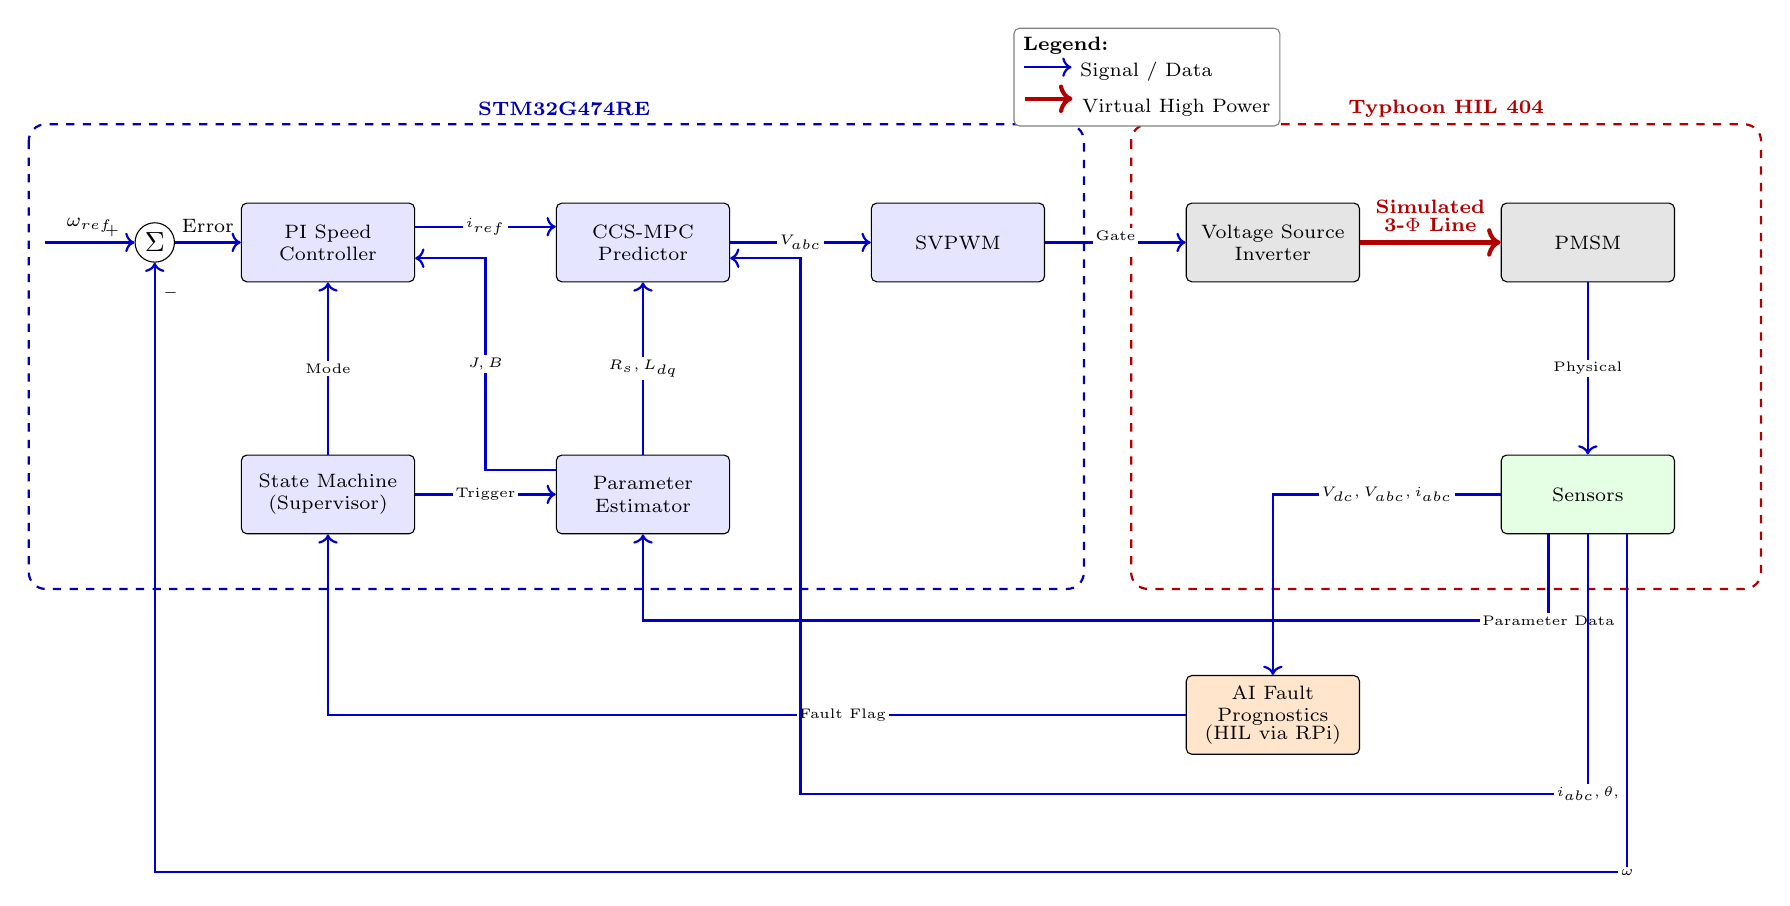
\begin{tikzpicture}[
    ctrlblock/.style={draw=black, fill=blue!10, rectangle, rounded corners=2pt, minimum width=2.2cm, minimum height=1cm, align=center, font=\scriptsize},
    powerblock/.style={draw=black, fill=gray!20, rectangle, rounded corners=2pt, minimum width=2.2cm, minimum height=1cm, align=center, font=\scriptsize},
    sensorblock/.style={draw=black, fill=green!10, rectangle, rounded corners=2pt, minimum width=2.2cm, minimum height=1cm, align=center, font=\scriptsize},
    aiblock/.style={draw=black, fill=orange!20, rectangle, rounded corners=2pt, minimum width=2.2cm, minimum height=1cm, align=center, font=\scriptsize},
    sum/.style={draw=black, circle, minimum size=0.5cm, inner sep=0pt},
    signal/.style={->, draw=blue!80!black, thick},
    power/.style={->, draw=red!70!black, line width=1.5pt},
    labelbox/.style={fill=white, inner sep=1pt, font=\tiny}
]
    \def\dx{4.0}
    \def\dy{-3.2}
    \draw[dashed, thick, draw=blue!70!black, rounded corners=6pt] (-3.8, 1.5) rectangle (9.6, -4.4);
    \node[text=blue!70!black, font=\scriptsize\bfseries] at (3.0, 1.7) { STM32G474RE};
    \draw[dashed, thick, draw=red!70!black, rounded corners=6pt] (10.2, 1.5) rectangle (18.2, -4.4);
    \node[text=red!70!black, font=\scriptsize\bfseries] at (14.2, 1.7) { Typhoon HIL 404 };
    \node[sum]         (sum)   at (-2.2, 0)     {$\Sigma$};
    \node[ctrlblock]   (pi)    at (0, 0)        {PI Speed\\Controller};
    \node[ctrlblock]   (mpc)   at (\dx, 0)      {CCS-MPC\\Predictor};
    \node[ctrlblock]   (svpwm) at (2*\dx, 0)    {SVPWM};
    \node[powerblock]  (inv)   at (3*\dx, 0)    {Voltage Source\\Inverter};
    \node[powerblock]  (motor) at (4*\dx, 0)    {PMSM};
    \node[ctrlblock]   (state) at (0, \dy)      {State Machine\\(Supervisor)};
    \node[ctrlblock]   (est)   at (\dx, \dy)    {Parameter\\Estimator};
    \node[sensorblock] (sense) at (4*\dx, \dy)  {Sensors};
    \node[aiblock]     (ai)    at (3*\dx, -6.0) {AI Fault\\Prognostics\\[-0.5ex]\scriptsize(HIL via RPi)};
    \node[draw=black!50, fill=white, rounded corners=2pt, align=left, font=\scriptsize] at (2.6*\dx, 2.1) {
        \textbf{Legend:}\\
        \tikz{\draw[signal] (0,0) -- (0.6,0);} Signal / Data\\
        \tikz{\draw[power]  (0,0) -- (0.6,0);} Virtual High Power
    };
    \draw[signal] (-3.6, 0) -- node[above, font=\scriptsize] {$\omega_{ref}$} node[pos=0.75, yshift=0.15cm] {\tiny $+$} (sum.west);
    \draw[signal] (sum.east) -- node[above, font=\scriptsize] {Error} (pi.west);
    \draw[signal] ([yshift=0.2cm]pi.east) -- node[labelbox] {$i_{ref}$} ([yshift=0.2cm]mpc.west);
    \draw[signal] (mpc) -- node[labelbox] {$V_{abc}$} (svpwm);
    \draw[signal] (svpwm) -- node[labelbox, align=center] {Gate\\[-0.5ex]} (inv);
    \draw[power]  (inv) -- node[above, font=\scriptsize\bfseries, text=red!70!black, align=center] {Simulated\\[-0.5ex]3-$\Phi$ Line} (motor);
    \draw[signal] (state) -- node[labelbox] {Mode} (pi);
    \draw[signal] (est) -- node[labelbox] {$R_s, L_{dq}$} (mpc);
    \draw[signal] (motor) -- node[labelbox] {Physical} (sense);
    \draw[signal] (state) -- node[labelbox] {Trigger} (est);
    \draw[signal] (sense.west) -| node[labelbox, pos=0.25] {$V_{dc}, V_{abc}, i_{abc}$} (ai.north);
    \draw[signal] (ai.west) -| node[labelbox, pos=0.2] {Fault Flag} (state.south);
    \draw[signal] ([yshift=-0.2cm]est.north west) -| node[labelbox, pos=0.75] {$J, B$} (2.0, -0.2) -- ([yshift=-0.2cm]pi.east);
    \draw[signal] ([xshift=-0.5cm]sense.south) |- (4.0, -4.8) node[labelbox, pos=0.5] {Parameter Data} -- (est.south);
    \draw[signal] (sense.south) |- (6.0, -7.0) node[labelbox, pos=0.5] { $i_{abc},\theta$,} |- ([yshift=-0.2cm]mpc.east);
    \draw[signal] ([xshift=0.5cm]sense.south) |- (-2.2, -8.0) node[labelbox, pos=0.5] { $\omega$} -- node[pos=0.95, xshift=0.2cm] {\tiny $-$} (sum.south);
    \end{tikzpicture}
    }
\end{frame}

\begin{frame}{7. Methodology -- The Simulation-to-HIL Pipeline}
    \footnotesize
    \begin{itemize}
        \item \textbf{O1 -- Simulation \& Estimation Setup:} Model PMSM in MATLAB/Simulink. Implement sequences to gather electrical and mechanical parameters dynamically, creating the baseline logic for the control loops.
        \item \textbf{O2 -- MIL \& SIL Verification:}
        \begin{itemize}
            \footnotesize
            \item \textbf{Model-in-the-Loop (MIL):} Validate the dual-loop auto-tuning control algorithm against continuous analytical plant models.
            \item \textbf{Software-in-the-Loop (SIL):} Utilize Embedded Coder to auto-generate C-code from the control logic. Execute this compiled code on the host PC to ensure algorithmic integrity before hardware deployment.
        \end{itemize}
        \item \textbf{O3 -- HIL Validation:} Interface the physical \textbf{STM32G474RE microcontroller} with the real-time plant emulator. The MCU executes the CCS-MPC and SVPWM natively, passing hardware gate signals to the simulator and receiving analog/digital feedback in real-time.
        \item \textbf{O4 -- Prognostics Deployment:} Inject controlled inverter switch-level faults via the HIL software interface. Utilize a \textbf{Raspberry Pi} to intercept the real-time analog signatures and execute the AI fault classification model, completing the diagnostic loop.
    \end{itemize}
\end{frame}

\begin{frame}{8. Parameter Identification \& Auto-Tuning Strategy}
    \footnotesize
    \begin{block}{1. Electrical Parameter Estimation (Standstill)}
        \begin{itemize}
            \item \textbf{Stator Resistance ($R_s$):} Apply a DC voltage pulse across the phases and measure the resulting steady-state current ($V/I$).
            \item \textbf{Inductances ($L_d, L_q$):} Inject high-frequency voltage pulses or step voltages to analyze the current rate-of-change ($di/dt$) along the $d$ and $q$ axes.
        \end{itemize}
    \end{block}
    
    \vspace{-1.5mm}
    \begin{block}{2. Mechanical Parameter \& Flux Estimation Sequence}
        \begin{itemize}
            \item \textbf{Step 1 - Flux Test ($\lambda_f$):} The drive spins the motor up open-loop, cuts the power, and measures the unpowered Back-EMF voltage coast-down to calculate $\lambda_f$.
            \item \textbf{Step 2 - Friction Test ($B$):} Now that it knows $\lambda_f$, it spins the motor back up to a constant speed. It measures $i_q$, calculates the exact $T_e$ it is generating, and divides that by the speed to find $B$.
            \item \textbf{Step 3 - Inertia Test ($J$):} From that constant speed, it cuts the torque to zero and watches how fast the motor decelerates to find $J$.
        \end{itemize}
    \end{block}

    \vspace{-1.5mm}
    \begin{block}{3. PI Speed Loop Auto-Tuning}
        \begin{itemize}
            \item The identified parameters dictate the outer speed controller tuning based on a desired closed-loop bandwidth ($\omega_c$).
            \item The PI gains are calculated.
        \end{itemize}
    \end{block}
\end{frame}

\begin{frame}{10. Supervisory Control: State Machine, Mode \& Trigger}
    \footnotesize
    \begin{block}{1. The State Machine Sequence}
        \vspace{-1mm}
        \begin{itemize}
            \item \textbf{State 0 (IDLE):} Waiting for start command, switches are OFF.
            \item \textbf{State 1 (STANDSTILL):} Injecting DC/AC pulses to find $R_s$ and $L_{dq}$.
            \item \textbf{State 2 (ALIGNMENT):} Locking the rotor to $\theta = 0$.
            \item \textbf{State 3 (OPEN-LOOP SPINUP):} Using Openloop control to reach steady speed.
            \item \textbf{State 4 (COAST-DOWN):} Switches OFF, measuring Back-EMF and deceleration.
            \item \textbf{State 5 (CALCULATE GAINS):} Computing $K_p, K_i$ and MPC matrices $A_d, B_d$.
            \item \textbf{State 6 (NORMAL RUN):} Closing the loops, standard MPC drive operation.
        \end{itemize}
        \vspace{-1mm}
    \end{block}
    \vspace{-1mm}
    \begin{columns}[T]
        \column{0.48\textwidth}
        \begin{block}{2. Mode Signal (To PI Controller)}
            \begin{itemize}
                \item \textbf{DISABLED:} Outputs zero (during standstill \& coast-down).
                \item \textbf{OVERRIDE:} Passes hardcoded open-loop torque limit (during spinup).
                \item \textbf{ACTIVE:} Uses auto-tuned gains.
            \end{itemize}
        \end{block}
        \column{0.48\textwidth}
        \begin{block}{3. Trigger Signal (To Estimator)}
            \begin{itemize}
                \item \textbf{Capture $R_s, L_{dq}$:} Triggered instantly during State 1 pulses.
                \item \textbf{Capture $\lambda_f, J, B$:} Triggered at exact moments in States 3 \& 4 to sync the math calculation with physical events.
            \end{itemize}
        \end{block}
    \end{columns}
\end{frame}

\begin{frame}{11. Expected Outcome -- What Success Looks Like}
    \begin{itemize}
        \item A working \textbf{self-commissioning algorithm} that estimates both electrical ($R_s, L_{dq}, \lambda_f$) and mechanical ($J, B$) parameters within an acceptable error margin
        \item An \textbf{Auto-tuned PI outer loop} and a \textbf{CCS-MPC inner current loop} (on STM32G474RE) that dynamically update their internal matrices based purely on self-identified data
        \item Demonstrated \textbf{reduction in commissioning time} compared to conventional manual-tuning workflows
        \item A comprehensive \textbf{Hardware-in-the-Loop testbed} demonstrating adaptive motor control interacting safely with high-fidelity simulated power stages
        \item An \textbf{AI-based prognostic module} capable of early detection of inverter switch-level (SVPWM) faults, fully deployed and validated on a \textbf{Raspberry Pi} during HIL fault-injection testing
    \end{itemize}
\end{frame}

\begin{frame}{12. Software and Hardware Requirements}
    \begin{columns}[T]
        \column{0.5\textwidth}
        \textbf{Software Toolchain}
        \begin{itemize}
            \footnotesize
            \item MATLAB / Simulink
            \item Simscape Electrical (for Plant Modeling)
            \item Stateflow (supervisory test logic)
            \item Embedded Coder (C-code generation)
            \item STM32CubeIDE (for MPC control flash)
            \item Python / TensorFlow (for AI prognostics on Raspberry Pi)
        \end{itemize}
        \column{0.5\textwidth}
        \textbf{Hardware \& Emulation}
        \begin{itemize}
            \footnotesize
            \item \textbf{Microcontroller (STM32G474RE)} for real-time cascaded control execution
            \item \textbf{Raspberry Pi} (for AI Prognostics deployment)
            \item Real-time HIL target (Typhoon 404 HIL)
            \item Interface logic shifters \& jumper cabling
            \item Oscilloscope / Logic Analyzer
        \end{itemize}
    \end{columns}
\end{frame}

\begin{frame}{13. Cost Estimate of the Project}
    \centering
    \small
    \begin{tabular}{l l r}
        \toprule
        \textbf{Item} & \textbf{Purpose} & \textbf{Approx. Cost (₹)} \\
        \midrule
        Microcontroller dev kit (STM32G474RE) & Real-time embedded control & 3,000 -- 5,000 \\
        Raspberry Pi kit & AI Prognostics Deployment & 4,000 -- 7,000 \\
        Interface Components & I/O shifting for HIL connection & 1,000 -- 2,000 \\
        HIL platform usage / lab access & Real-time plant emulation & As per lab availability \\
        \midrule
        \textbf{Estimated Total} & & \textbf{₹8,000 -- 14,000} \\
        \bottomrule
    \end{tabular}
    \vspace{0.3cm}
    
    \textit{*Note: By focusing on HIL validation rather than a physical high-voltage power stage, prototype costs and hardware risk are significantly minimized while preserving control complexity.}
\end{frame}

\begin{frame}{14. Time Frame for Execution (8 Months)}
    \centering
    \resizebox{\textwidth}{!}{%
    \begin{tabular}{l*{8}{c}}
        \toprule
        \textbf{Task} & M1 & M2 & M3 & M4 & M5 & M6 & M7 & M8 \\
        \midrule
        Lit. survey \& topic finalization & \cellcolor{blue!40} & & & & & & & \\
        Standstill ID \& Low-Speed ID logic & \cellcolor{blue!40} & \cellcolor{blue!40} & & & & & & \\
        CCS-MPC integration \& simulation & & \cellcolor{blue!40} & \cellcolor{blue!40} & & & & & \\
        MIL testing \& PI Auto-tuning & & & \cellcolor{blue!40} & & & & & \\
        SIL testing (C-code generation) & & & \cellcolor{blue!40} & \cellcolor{blue!40} & & & & \\
        HIL setup \& STM32 interfacing & & & & \cellcolor{blue!40} & \cellcolor{blue!40} & & & \\
        HIL validation of Auto-tuning drive & & & & & \cellcolor{blue!40} & \cellcolor{blue!40} & & \\
        HIL Inverter Fault Injection sequencing & & & & & & \cellcolor{blue!40} & & \\
        AI Prognostics Training with Rasberry Pi \& Integration & & & & & & \cellcolor{blue!40} & \cellcolor{blue!40} & \\
        Final HIL System Demo & & & & & & & \cellcolor{blue!40} & \cellcolor{blue!40} \\
        Documentation \& final review & & & & & & & & \cellcolor{blue!40} \\
        \bottomrule
    \end{tabular}}
    \vspace{0.2cm}
    \scriptsize Semester 1: M1--M4 (Algorithm + MIL + SIL) \quad Semester 2: M5--M8 (HIL Interfacing + AI Prognostics + Final Validation)
\end{frame}

\begin{frame}{15. References (IEEE Format)}
    \tiny
    \textbf{Base Paper:} I. Hammoud \textit{et al.}, ``On Continuous-Set Model Predictive Control of Permanent Magnet Synchronous Machines,'' \textit{IEEE Trans. Power Electron.}, vol. 37, no. 9, Sept. 2022.
    \vspace{2mm}
    \begin{thebibliography}{9}
        \bibitem{1} M. S. Rafaq and J. Jung, ``A Comprehensive Review of State-of-the-Art Parameter Estimation Techniques for PMSM,'' \textit{IEEE Trans. Ind. Inform.}, vol. 16, no. 7, 2020.
        \bibitem{2} N. Rajeswaran \textit{et al.}, ``FPGA Implementation of AI-Based Inverter IGBT Open Circuit Fault Diagnosis,'' \textit{Micromachines}, vol. 13, no. 5, 2022.
        \bibitem{3} A. Bacha \textit{et al.}, ``Advanced Deep Learning Approaches for Fault Detection and Diagnosis in Inverter-Driven PMSM Systems,'' \textit{IJACSA}, vol. 15, no. 12, 2024.
        \bibitem{4} W. Zhao \textit{et al.}, ``Continuous Control Set Predictive Control with Affine Registration Technique for PMSM Drive,'' \textit{Energies}, vol. 17, no. 18, 2024.
        \bibitem{5} Z. Liu \textit{et al.}, ``Global Identification of Electrical and Mechanical Parameters in PMSM Drive Based on Dynamic Self-Learning PSO,'' \textit{IEEE Trans. Power Electron.}, vol. 33, no. 12, 2018.
        \bibitem{6} P. Carlet \textit{et al.}, ``Real-Time Feasibility of Data-Driven Predictive Control for Synchronous Motor Drives,'' \textit{IEEE Trans. Power Electron.}, vol. 38, no. 2, 2023.
        \bibitem{7} Z. Liang \textit{et al.}, ``Weight-Adaptable Disturbance Observer for CCS-MPC of NPC-3L-Fed PMSMS,'' \textit{Energies}, vol. 18, no. 21, 2025.
        \bibitem{8} Y. Zhang \textit{et al.}, ``An open-circuit fault diagnosis method for PMSM drive system based on multi-branch 1D-CNN,'' \textit{J. Phys.: Conf. Ser.}, 2024.
        \bibitem{9} L. Li \textit{et al.}, ``Mechanism-Based Fault Diagnosis Deep Learning Method for PMSM,'' \textit{Sensors}, vol. 24, no. 19, 2024.
    \end{thebibliography}
\end{frame}

% ===================================================
%                 FIRST REVIEW (NEW SLIDES)
% ===================================================

\begin{frame}
    \centering
    \vfill
    \Huge \textbf{First Review}
    \vfill
    \normalsize Progress \& Architecture Analysis
\end{frame}

\begin{frame}{16. The Industry Problem \& Our Solution}
    \begin{itemize}
        \item \textbf{The Industry Standard:} Permanent Magnet Synchronous Motors (PMSMs) dominate EV traction and industrial automation due to high efficiency. However, their drives rely almost entirely on Field-Oriented Control (FOC) governed by manually tuned PI controllers.
        \item \textbf{The Bottleneck:} Whenever a motor is swapped on an assembly line, technicians must halt production to manually re-tune the $K_p$ and $K_i$ gains to match the new motor's specific electrical and mechanical traits.
        \item \textbf{Why CCS-MPC for PMSM:} PMSMs exhibit highly coupled, non-linear d-q axis dynamics (especially at high speeds). CCS-MPC explicitly handles these cross-couplings and multi-variable constraints analytically, enabling superior transient response without cascaded PI tuning.
        \item \textbf{Our Proposed Solution:} 
        \begin{enumerate}
            \item Replace the rigid FOC current loops with a \textbf{Continuous Control Set Model Predictive Control (CCS-MPC)} algorithm that analytically calculates optimal voltages.
            \item Introduce an \textbf{AutoTuner State Machine} to autonomously execute pre-operational self-commissioning (extracting $R_s, L_d, L_q, \Psi_{PM}, J, B$) and directly feed them to the MPC, enabling true plug-and-play capability.
        \end{enumerate}
    \end{itemize}
\end{frame}

\begin{frame}{16a. Plant Model: Power Stage }
    \centering
    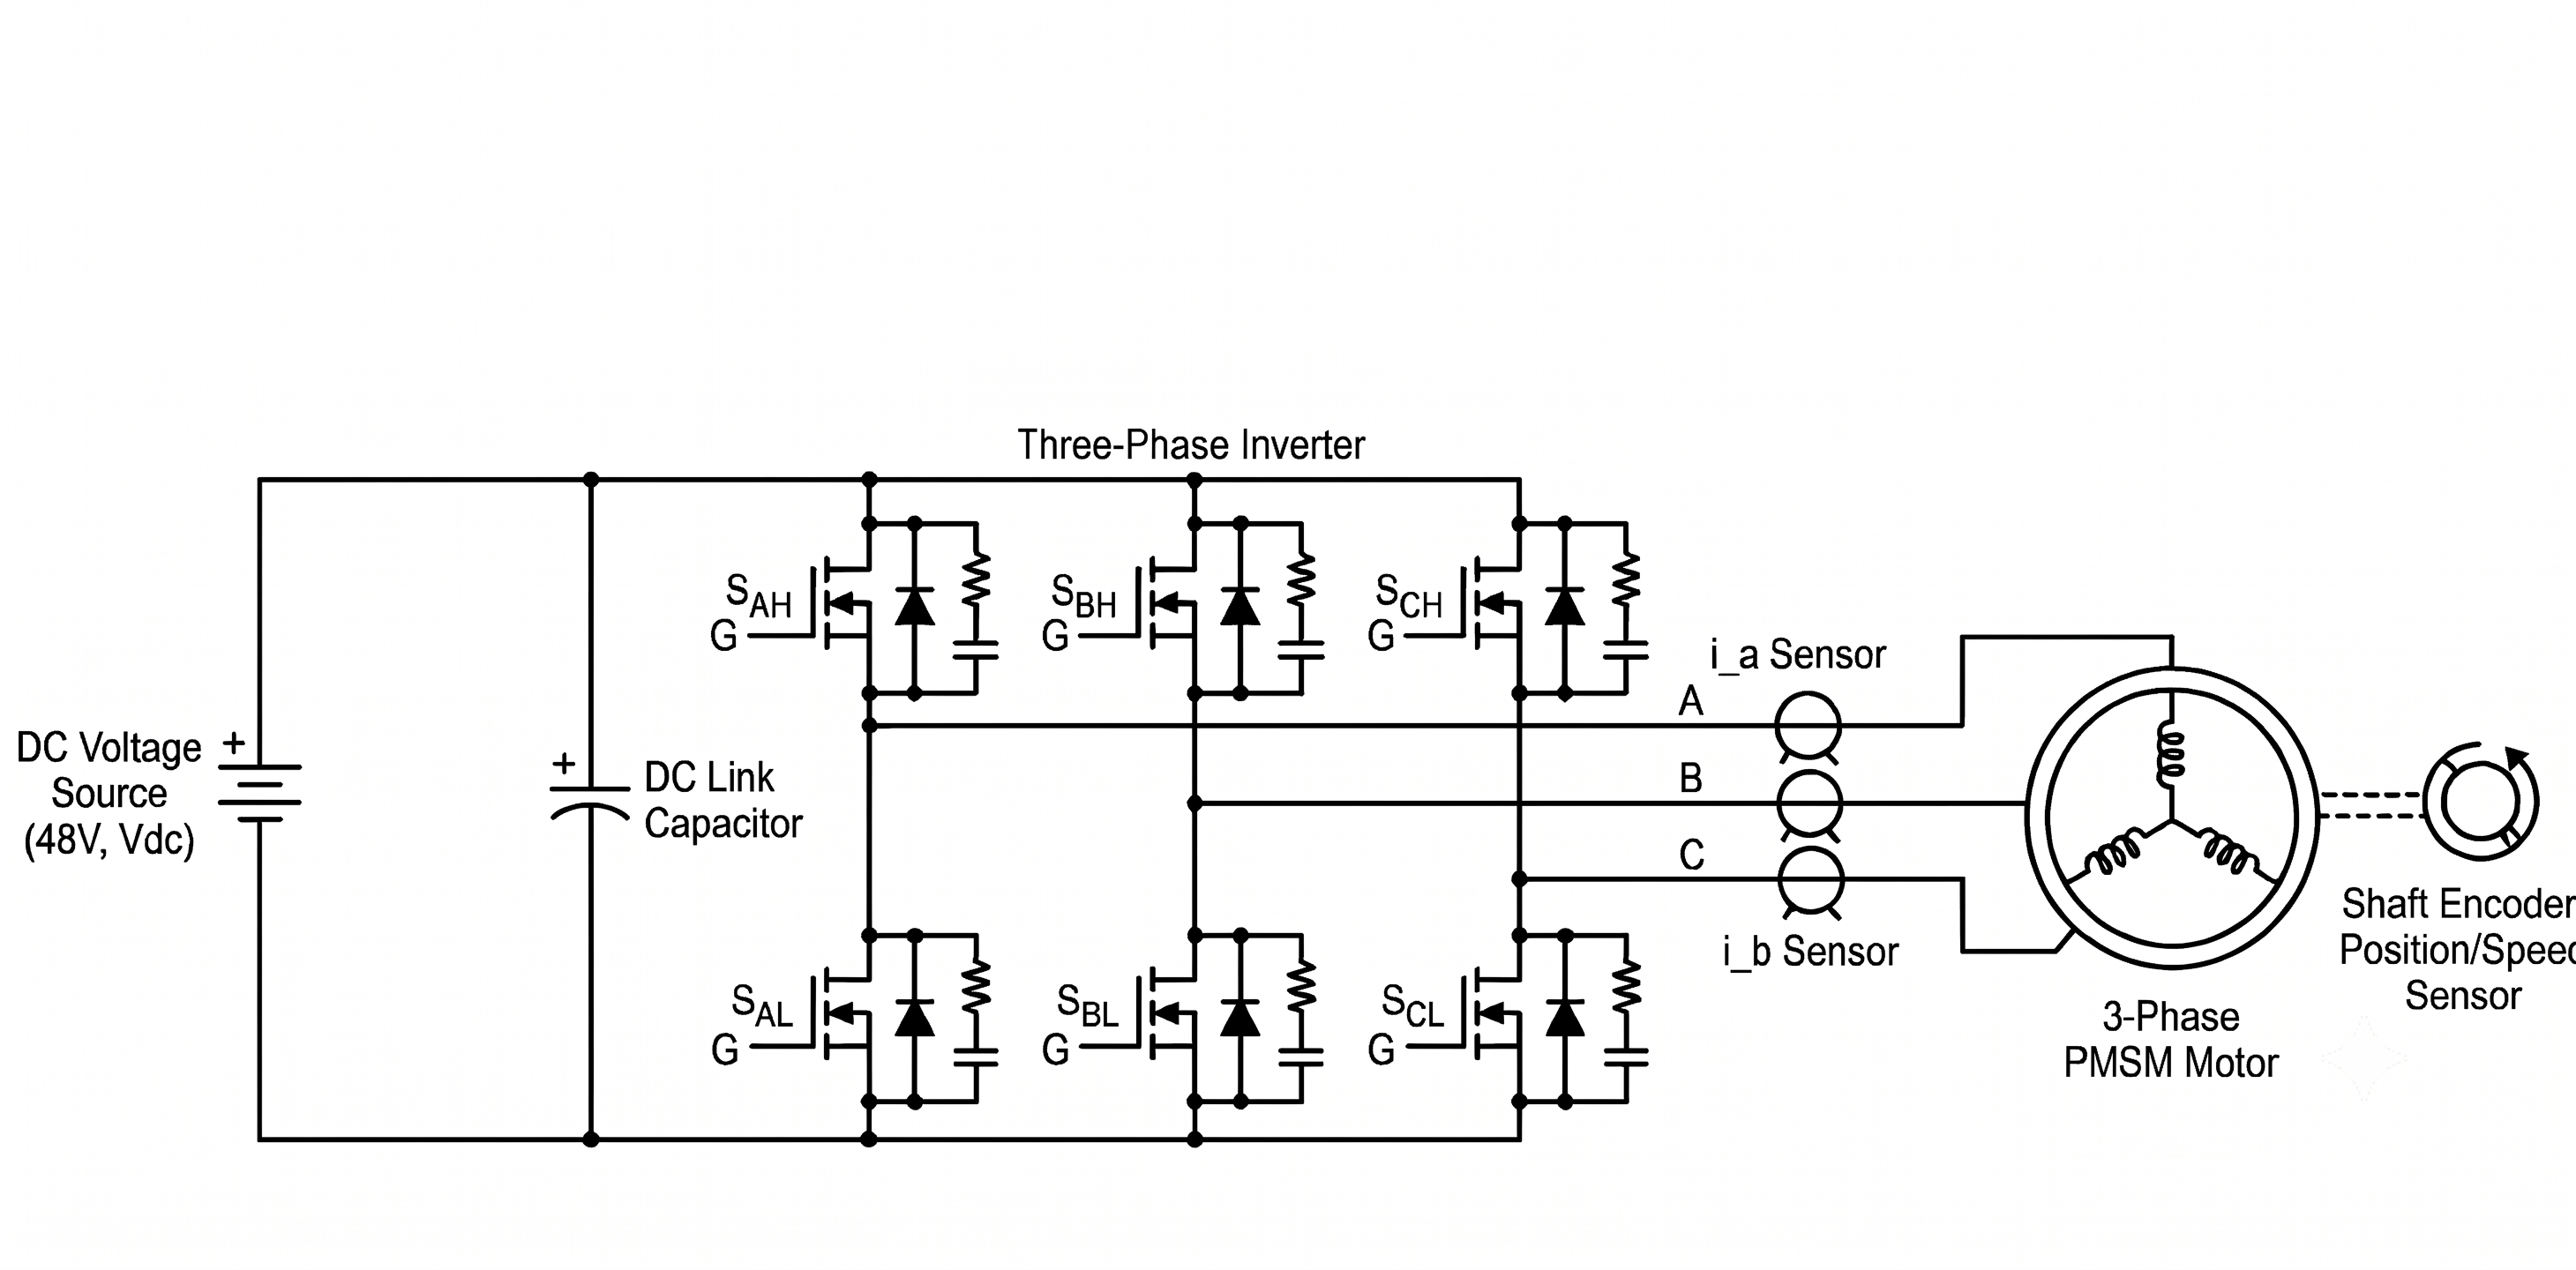
\includegraphics[height=0.9\textheight,keepaspectratio]{Gemini_Generated_Image_74ckp974ckp974ck (1).png}
    \vspace{2mm}
\end{frame}

\begin{frame}{16b. System Parameters (Plant \& Controller)}
    \vspace{-2mm}
    \footnotesize
    \begin{columns}[T]
        \column{0.52\textwidth}
        \textbf{PMSM \& Inverter Parameters} \\
        \textit{\scriptsize Standard Application: BMW i3 Traction Motor (EV) \cite{6}}
        \vspace{1mm}

        \resizebox{\linewidth}{!}{%
        \renewcommand{\arraystretch}{1.2}
        \begin{tabular}{llc}
            \toprule
            \textbf{Parameter} & \textbf{Symbol} & \textbf{Value} \\
            \midrule
            \rowcolor{blue!5} Nominal DC Bus Voltage & $V_{dc}$ & 275.7 V \\
            MOSFET On-Resistance & $R_{on}$ & 1.0 m$\Omega$ \\
            \rowcolor{blue!5} Switching Frequency & $f_{sw}$ & 10 kHz \\
            Stator Resistance & $R_s$ & 5.3 m$\Omega$ \\
            \rowcolor{blue!5} d/q-axis Inductance & $L_d, L_q$ & 71.2 $\mu$H, 141.3 $\mu$H \\
            PM Flux Linkage & $\Psi_{PM}$ & 0.0436 Wb \\
            \rowcolor{blue!5} Pole Pairs & $p$ & 6 \\
            Rotor Inertia & $J$ & 0.0867 kg$\cdot$m$^2$ \\
            \rowcolor{blue!5} Viscous Friction & $B_{fric}$ & 0.001 N$\cdot$m$\cdot$s/rad \\
            Torque Constant & $K_t$ & 0.392 N$\cdot$m/A \\
            \rowcolor{blue!5} Peak Torque & $T_{rated}$ & 258.2 N$\cdot$m \\
            \bottomrule
        \end{tabular}%
        }

        \column{0.48\textwidth}
        \textbf{Control Loop \& Simulation}
        \vspace{1mm}

        \resizebox{\linewidth}{!}{%
        \renewcommand{\arraystretch}{1.2}
        \begin{tabular}{llc}
            \toprule
            \textbf{Parameter} & \textbf{Symbol} & \textbf{Value} \\
            \midrule
            \rowcolor{green!10} Control Sample Time & $T_{s,ctrl}$ & 100 $\mu$s \\
            Simulation Time Step & $T_{s,sim}$ & 5 $\mu$s \\
            \rowcolor{green!10} Speed PI Gains & $K_{p,spd}, K_{i,spd}$ & 2.0, 10.0 \\
            Current PI Bandwidth & $\omega_{c,curr}$ & $2\pi \times 1000$ rad/s \\
            \rowcolor{green!10} Max Phase Current & $I_{peak}$ & 565.7 A \\
            CCS-MPC Error Weights & $Q_{id}, Q_{iq}$ & 1.0, 1.0 \\
            \rowcolor{green!10} CCS-MPC Switch Weight & $R_{sw}$ & 0.001 \\
            Max Phase Voltage & $V_{ph,max}$ & 159.2 V \\
            \rowcolor{green!10} Inverter Deadtime & $T_{dead}$ & 2 $\mu$s \\
            \bottomrule
        \end{tabular}%
        }
    \end{columns}
    \vspace{4mm}
    \begin{flushright}
        \tiny \textit{Note: Parameters verified via Comparative Analysis of Steady-State Models \cite{6}.}
    \end{flushright}
\end{frame}

% --- SLIDE 17: NEW FOC DIAGRAM ---
\begin{frame}{17. Conventional Field-Oriented Control (FOC) Architecture}
    \centering
    \vspace{2mm}
    \resizebox{\textwidth}{!}{%
    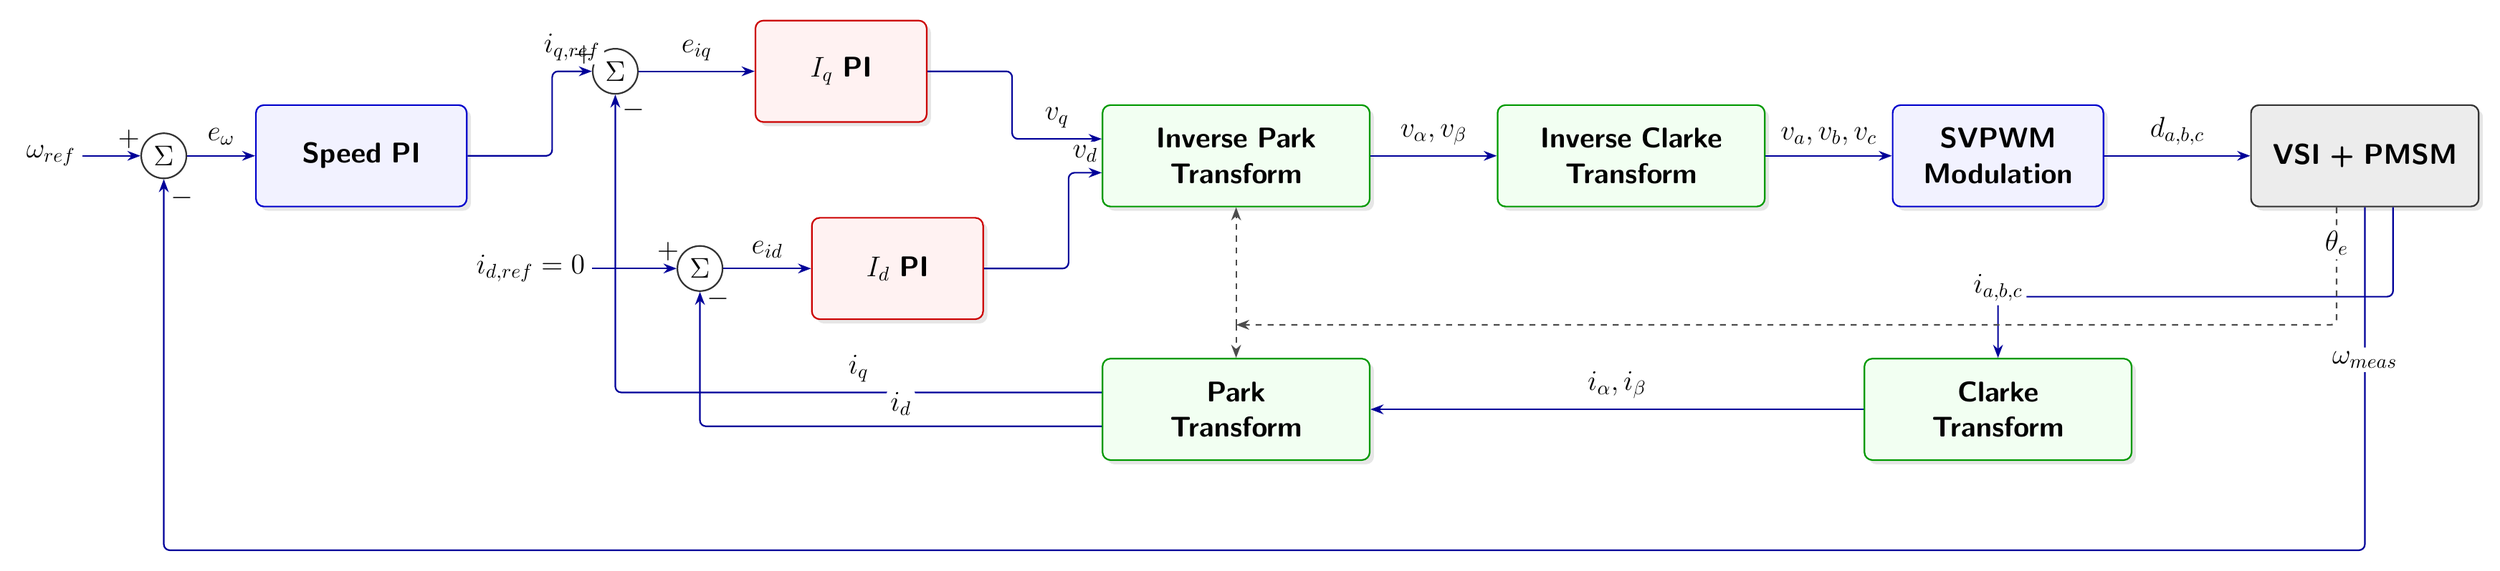
\begin{tikzpicture}[
        >=Stealth,
        every node/.style={font=\sffamily},
        common/.style={rectangle, draw=blue!80!black, fill=blue!5, thick, rounded corners=4pt, align=center, minimum height=1.8cm, text width=3.5cm, drop shadow={opacity=0.2}, font=\sffamily\Large},
        transform/.style={rectangle, draw=green!60!black, fill=green!5, thick, rounded corners=4pt, align=center, minimum height=1.8cm, text width=4.5cm, drop shadow={opacity=0.2}, font=\sffamily\Large},
        plant/.style={rectangle, draw=black!80, fill=gray!15, thick, rounded corners=4pt, align=center, minimum height=1.8cm, text width=3.8cm, drop shadow={opacity=0.2}, font=\sffamily\Large},
        focpi/.style={rectangle, draw=red!80!black, fill=red!5, thick, rounded corners=4pt, align=center, minimum height=1.8cm, text width=2.8cm, drop shadow={opacity=0.2}, font=\sffamily\Large},
        sum/.style={circle, draw=black!80, fill=white, thick, minimum size=0.8cm, inner sep=0pt, font=\Large},
        line/.style={->, thick, draw=blue!60!black, rounded corners=3pt},
        dashedline/.style={->, thick, dashed, draw=black!70, rounded corners=3pt},
        siglabel/.style={midway, above, yshift=3pt, font=\Large, fill=white, inner sep=2pt}
    ]

    % --- Forward Path Nodes ---
    \node[font=\Large] (w_ref) at (0, 0) {$\omega_{ref}$};
    \node[sum] (sum_w) at (2.0, 0) {$\Sigma$};
    \node[common] (speed_pi) at (5.5, 0) {\textbf{Speed PI}};

    \node[font=\Large] (id_ref) at (8.5, -2.0) {$i_{d,ref}=0$};
    \node[sum] (sum_q) at (10.0, 1.5) {$\Sigma$};
    \node[sum] (sum_d) at (11.5, -2.0) {$\Sigma$};

    \node[focpi] (iq_pi) at (14.0, 1.5) {$I_q$ \textbf{PI}};
    \node[focpi] (id_pi) at (15.0, -2.0) {$I_d$ \textbf{PI}};

    \node[transform] (inv_park) at (21.0, 0) {\textbf{Inverse Park} \\ \textbf{Transform}};
    \node[transform] (inv_clarke) at (28.0, 0) {\textbf{Inverse Clarke} \\ \textbf{Transform}};
    \node[common] (svpwm) at (34.5, 0) {\textbf{SVPWM} \\ \textbf{Modulation}};
    \node[plant] (plant) at (41.0, 0) {\textbf{VSI + PMSM}};

    % --- Feedback Path Nodes ---
    \node[transform] (clarke) at (34.5, -4.5) {\textbf{Clarke} \\ \textbf{Transform}};
    \node[transform] (park) at (21.0, -4.5) {\textbf{Park} \\ \textbf{Transform}};


    % --- FOC Connections ---
    \draw[line] (w_ref) -- (sum_w) node[pos=0.8, above, font=\Large] {$+$};
    \draw[line] (sum_w) -- (speed_pi) node[siglabel] {$e_\omega$};

    \draw[line] (speed_pi.east) -- ++(1.5, 0) |- (sum_q.west) node[pos=0.75, above, yshift=3pt, font=\Large, fill=white, inner sep=2pt] {$i_{q,ref}$} node[pos=0.9, above, font=\Large] {$+$};
    \draw[line] (id_ref) -- (sum_d.west) node[pos=0.9, above, font=\Large] {$+$};

    \draw[line] (sum_q.east) -- (iq_pi.west) node[siglabel] {$e_{iq}$};
    \draw[line] (sum_d.east) -- (id_pi.west) node[siglabel] {$e_{id}$};

    \draw[line] (iq_pi.east) -- ++(1.5, 0) |- ([yshift=3mm]inv_park.west) node[near end, above, yshift=3pt, font=\Large, fill=white, inner sep=2pt] {$v_q$};
    \draw[line] (id_pi.east) -- ++(1.5, 0) |- ([yshift=-3mm]inv_park.west) node[near end, above, yshift=3pt, font=\Large, fill=white, inner sep=2pt] {$v_d$};

    \draw[line] (inv_park.east) -- (inv_clarke.west) node[siglabel] {$v_\alpha, v_\beta$};
    \draw[line] (inv_clarke.east) -- (svpwm.west) node[siglabel] {$v_a, v_b, v_c$};
    \draw[line] (svpwm.east) -- (plant.west) node[siglabel] {$d_{a,b,c}$};

    % Feedback routing
    \draw[line] ([xshift=5mm]plant.south) |- (34.5, -2.5) -- (clarke.north) node[near start, above, yshift=3pt, font=\Large, fill=white, inner sep=2pt] {$i_{a,b,c}$};
    \draw[line] (clarke.west) -- (park.east) node[siglabel] {$i_\alpha, i_\beta$};

    \draw[line] ([yshift=3mm]park.west) -- (10.0, -4.2) node[midway, above, yshift=3pt, font=\Large, fill=white, inner sep=2pt] {$i_q$} -- (sum_q.south) node[pos=0.95, right, font=\Large] {$-$};
    \draw[line] ([yshift=-3mm]park.west) -- (11.5, -4.8) node[midway, above, yshift=3pt, font=\Large, fill=white, inner sep=2pt] {$i_d$} -- (sum_d.south) node[pos=0.95, right, font=\Large] {$-$};

    \draw[line] (plant.south) |- (2.0, -7.0) node[near start, above, yshift=3pt, font=\Large, fill=white, inner sep=2pt] {$\omega_{meas}$} -- (sum_w.south) node[pos=0.95, right, font=\Large] {$-$};

    % Theta routing
    \draw[dashedline] ([xshift=-5mm]plant.south) |- (21.0, -3.0) node[near start, above, yshift=3pt, font=\Large, fill=white, inner sep=2pt] {$\theta_e$};
    \draw[dashedline] (21.0, -3.0) -- (inv_park.south);
    \draw[dashedline] (21.0, -3.0) -- (park.north);
    \end{tikzpicture}%
    }
\end{frame}

%%% >>> FOC RESULT SLIDES INSERTED HERE <<<

\begin{frame}{17a. FOC Simulation Results -- Constant Speed: Current Tracking}
    \centering
    \begin{columns}[T]
        \column{0.5\textwidth}
        \centering
        \textbf{\small $I_q$ Tracking}\\[1mm]
        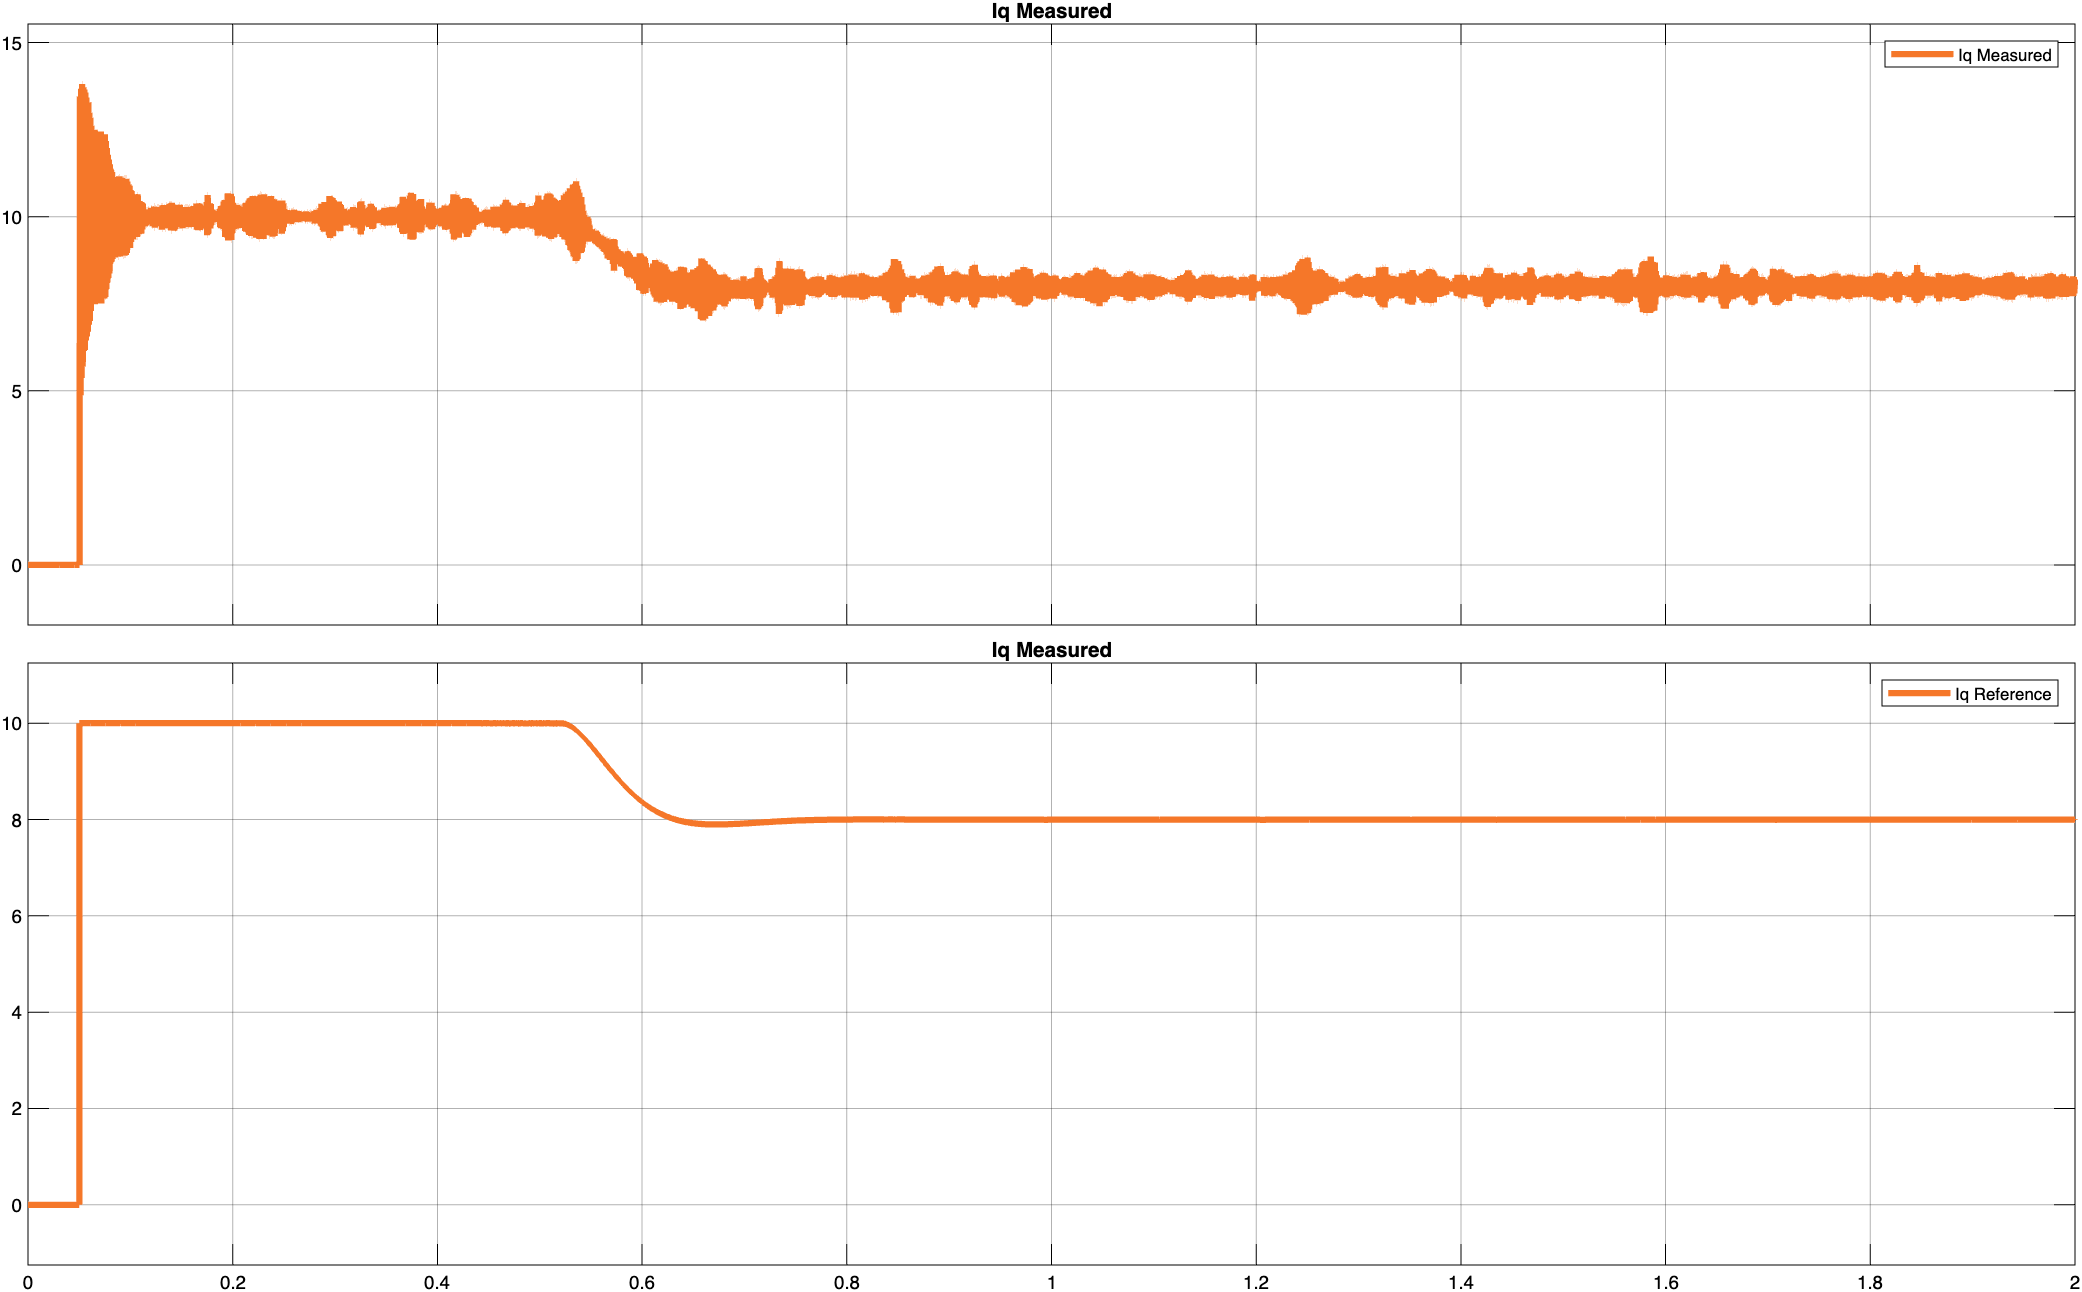
\includegraphics[width=\linewidth]{Iqcomp_FOC.png}
        \column{0.5\textwidth}
        \centering
        \textbf{\small $V_d, V_q$ Tracking}\\[1mm]
        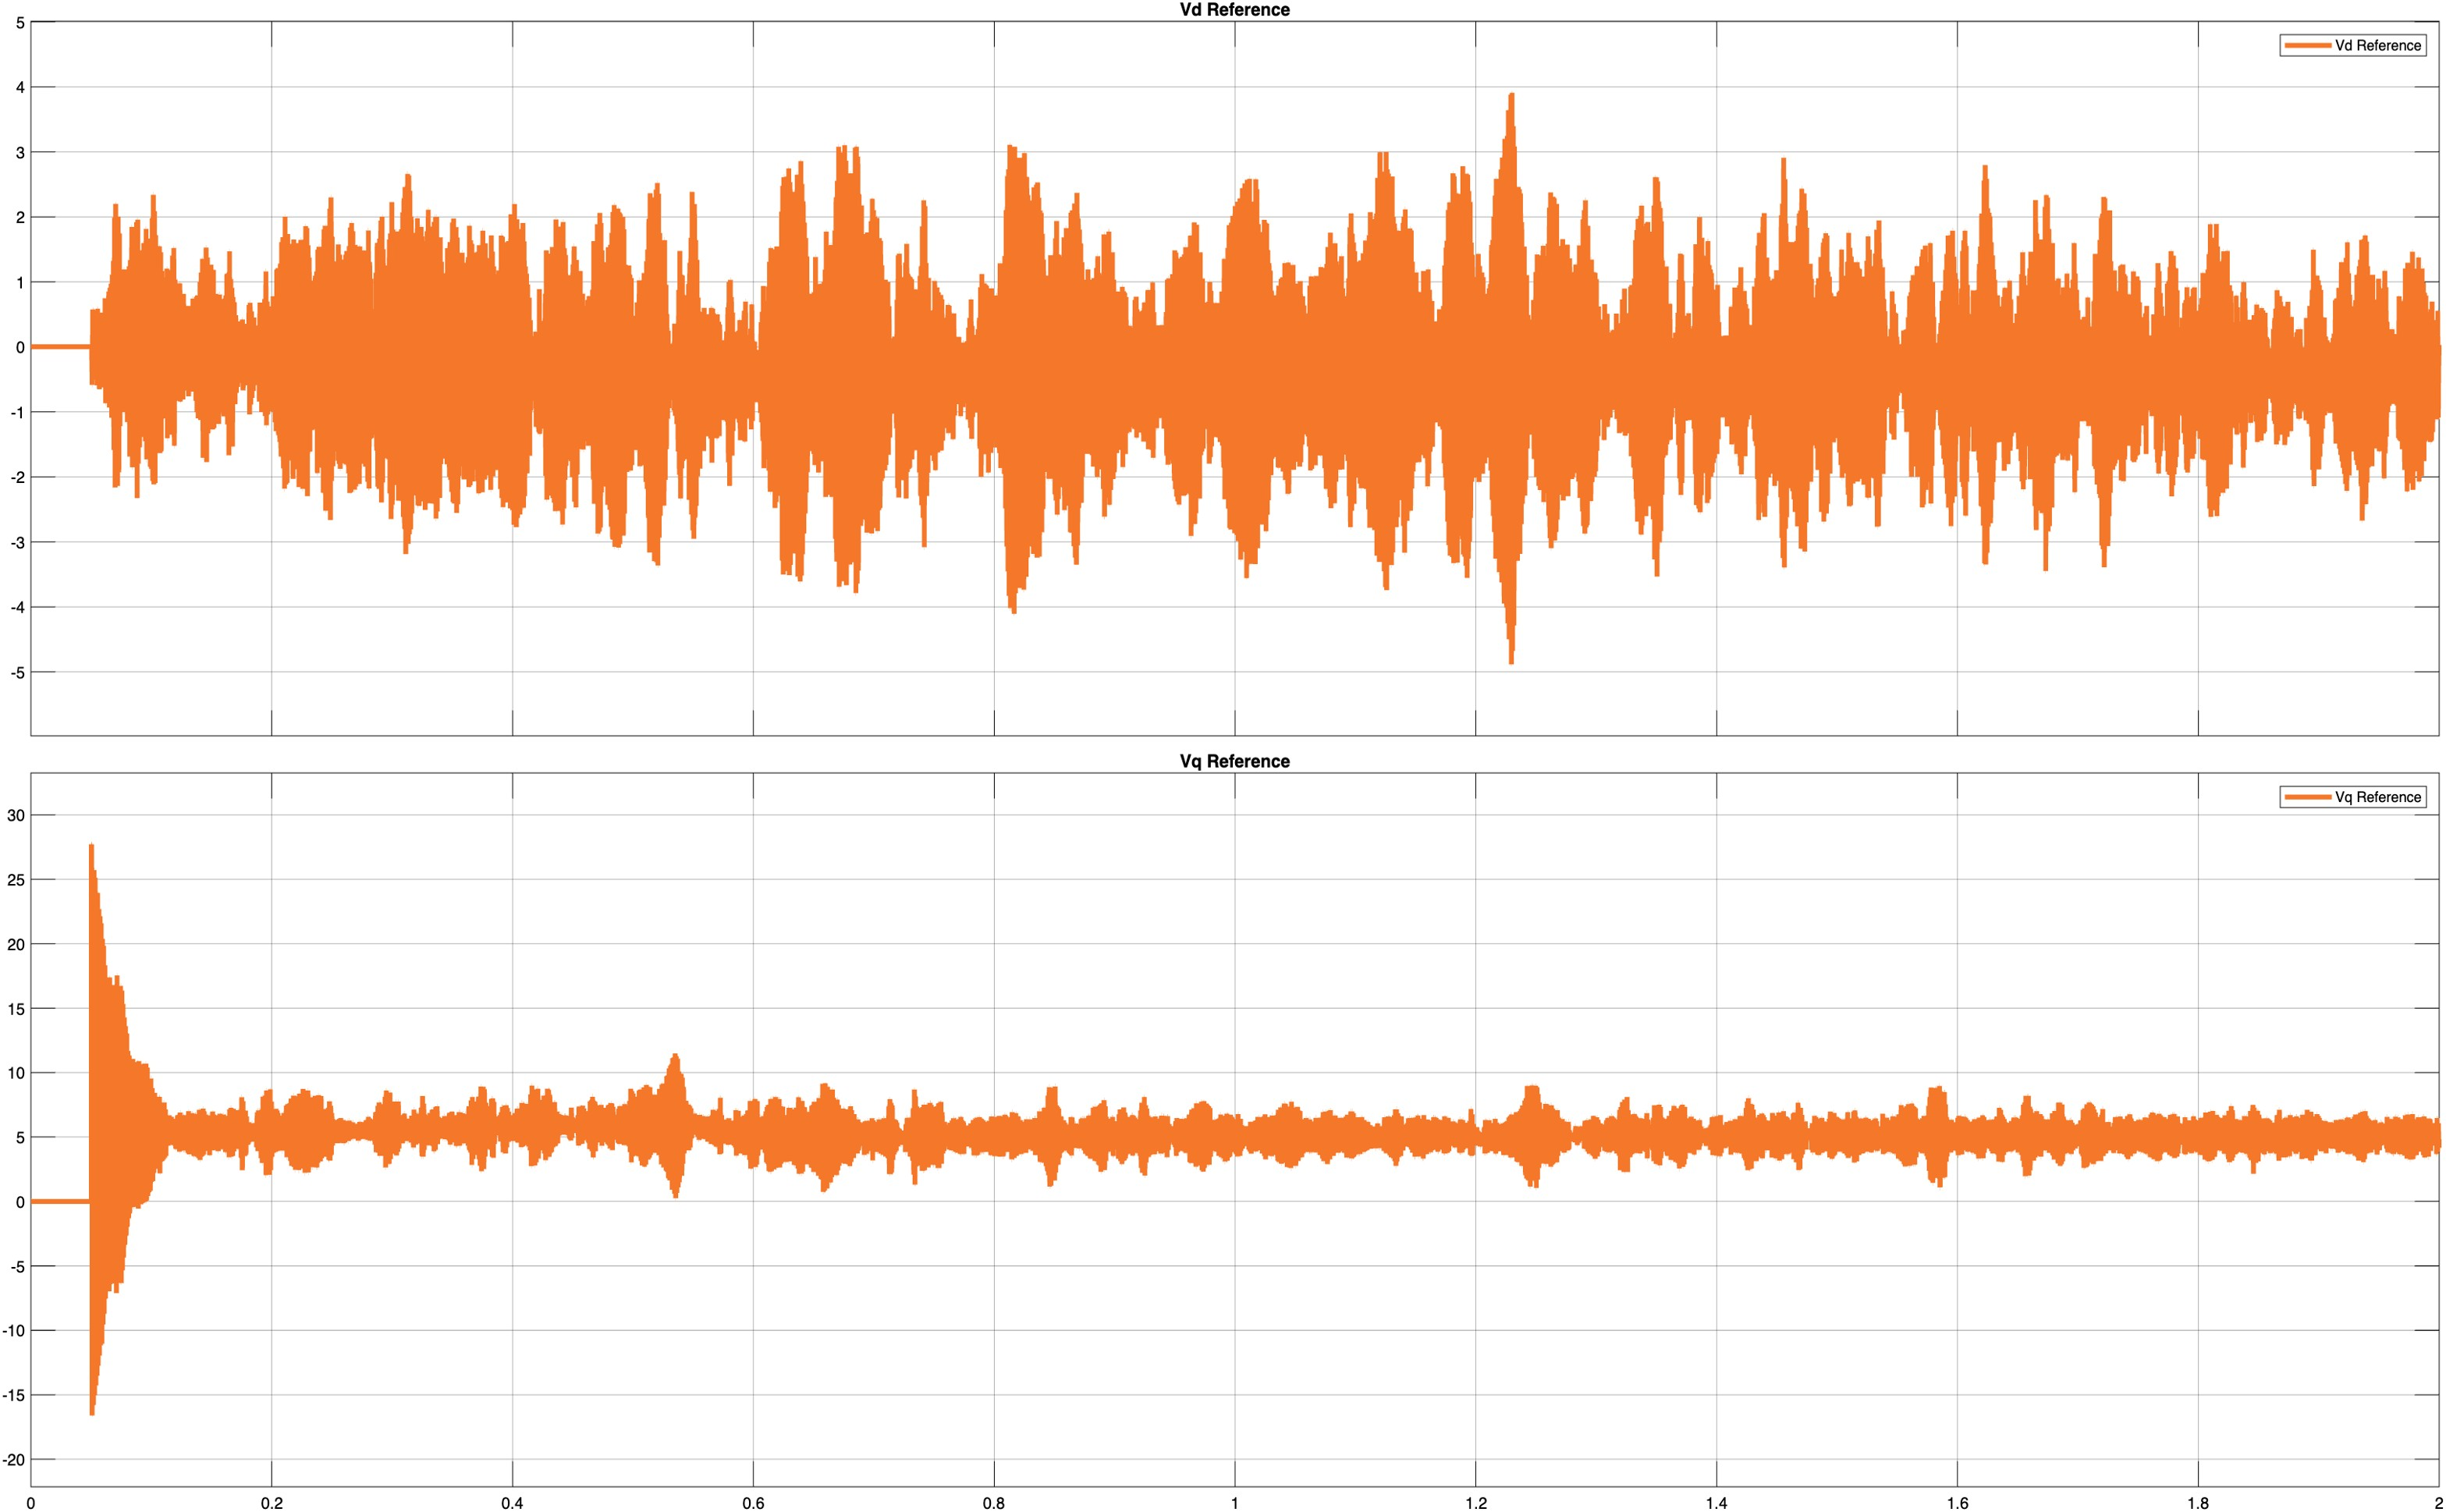
\includegraphics[width=\linewidth]{vd_vq_const.jpeg}
    \end{columns}
    \vspace{2mm}
    \begin{itemize}
        \item \textbf{Current Tracking Dynamics:} FOC current tracking under constant speed reference shows visible ripple on both axes due to cascaded PI loop delays and cross-axis coupling.
    \end{itemize}
\end{frame}

\begin{frame}{17b. FOC Simulation Results -- Constant Speed: Switching \& Speed}
    \centering
    \begin{columns}[T]
        \column{0.5\textwidth}
        \centering
        \textbf{\small Switching Pulses ($S_a, S_b, S_c$)}\\[1mm]
        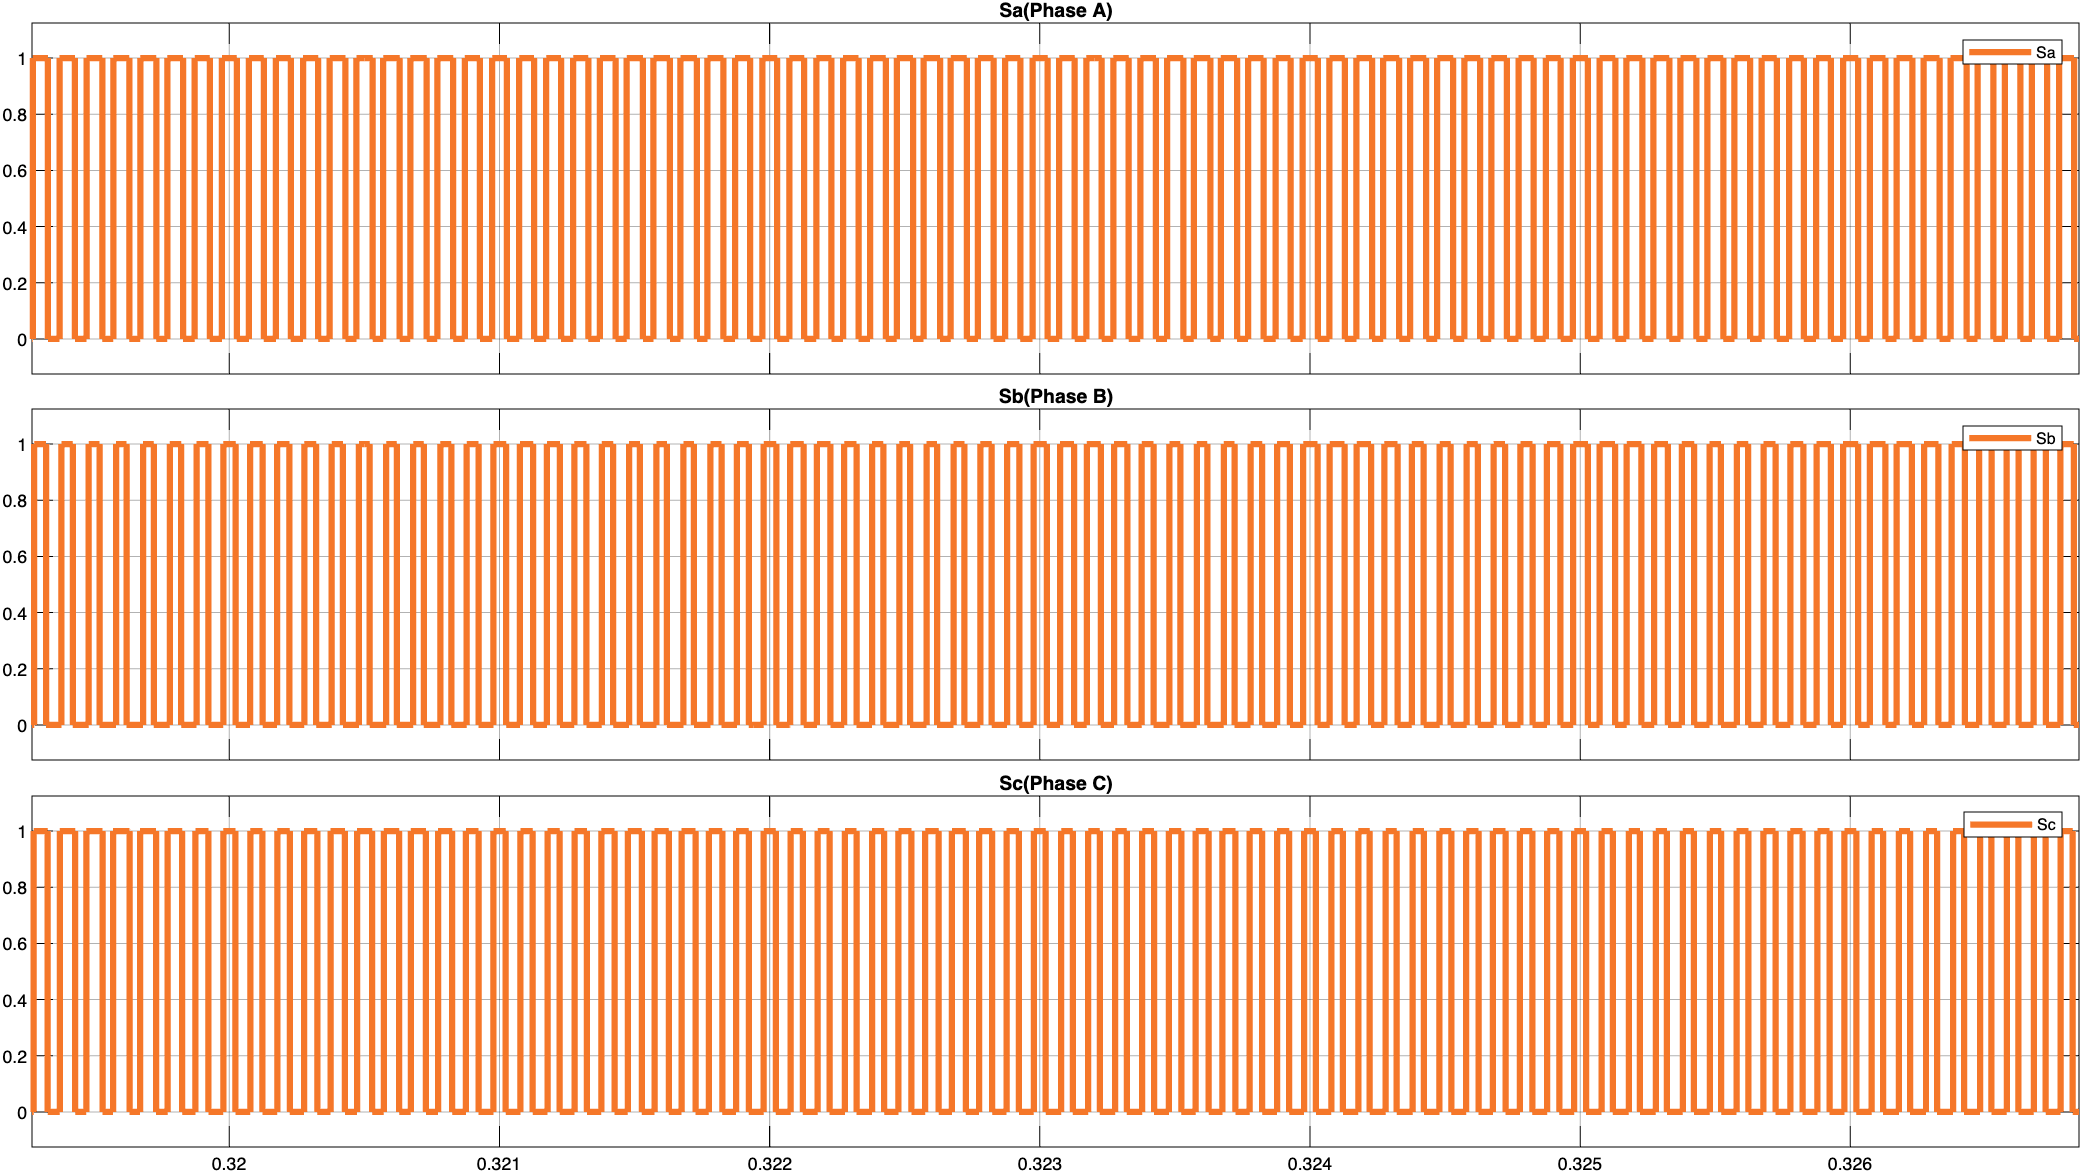
\includegraphics[width=\linewidth]{Sa_Sb_Sc_FOC.png}
        \column{0.5\textwidth}
        \centering
        \textbf{\small Speed Tracking}\\[1mm]
        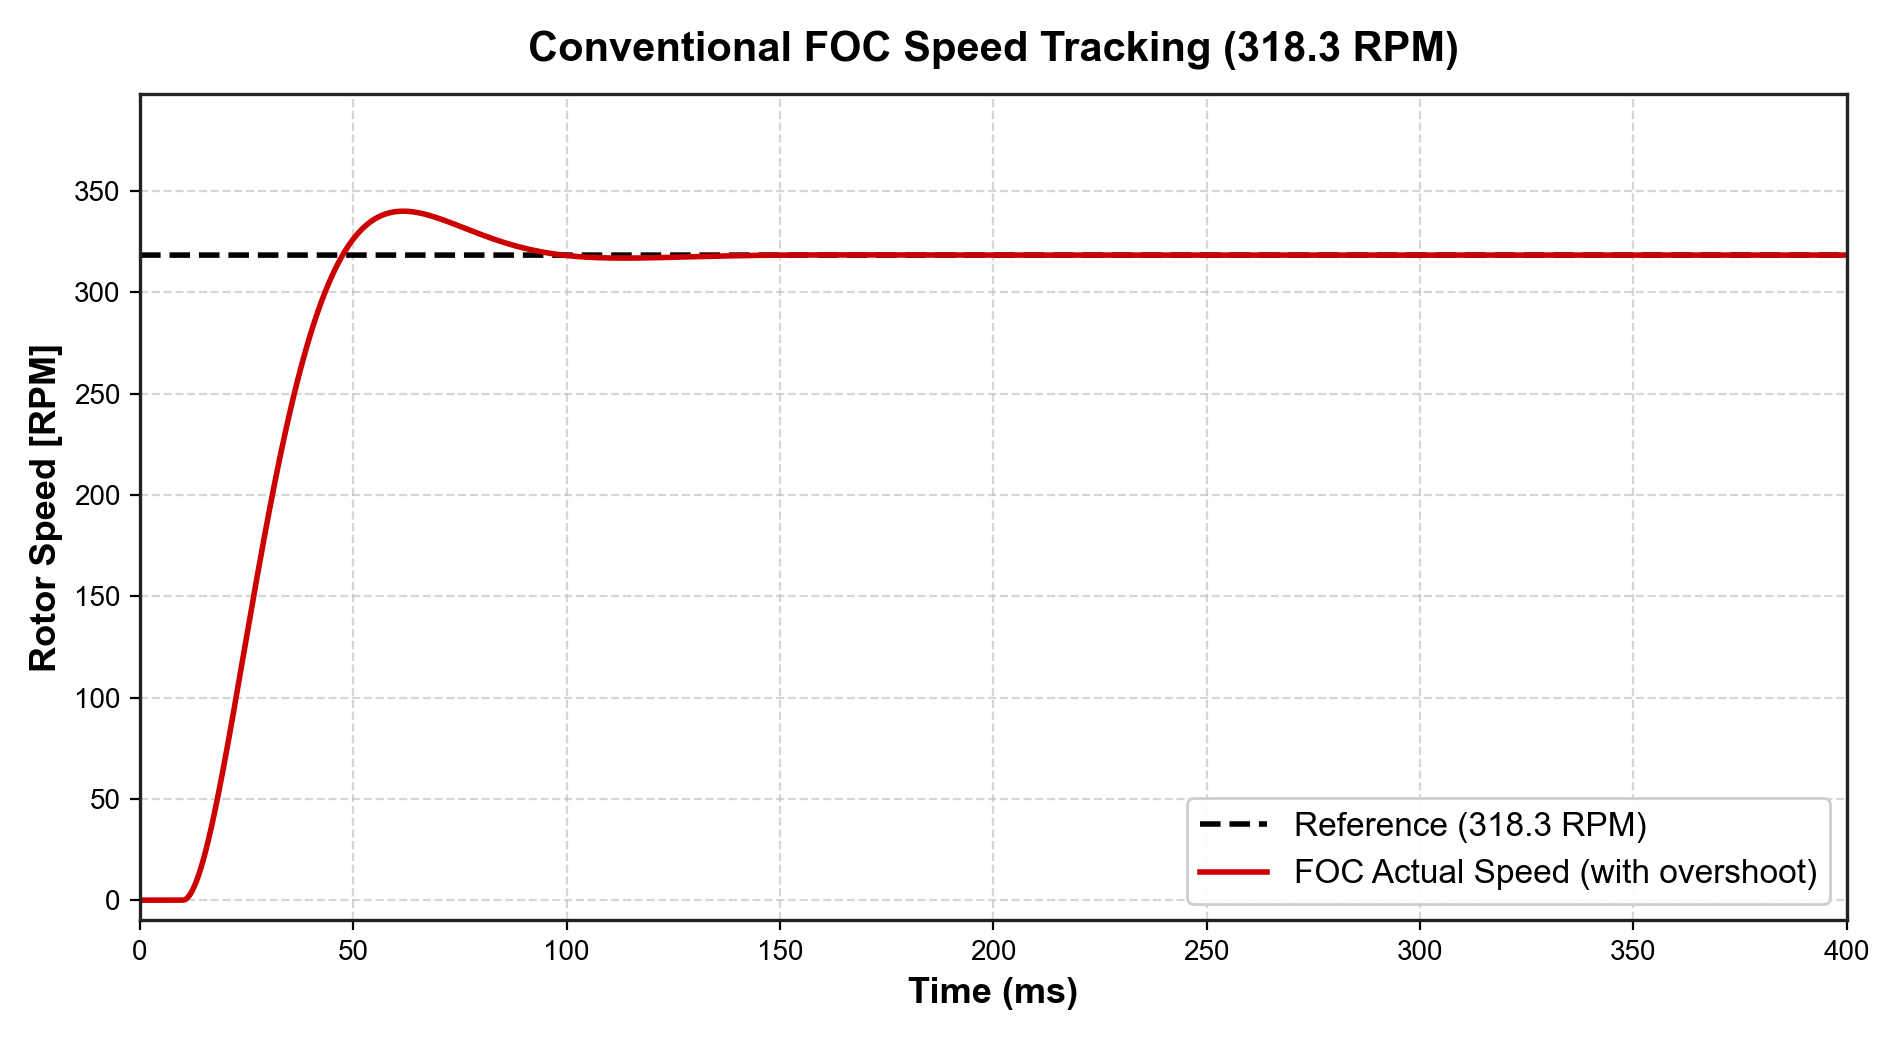
\includegraphics[width=\linewidth]{speed_comp_FOC.png}
    \end{columns}
    \vspace{2mm}
    \begin{itemize}
        \item \textbf{Speed Response:} The FOC speed response settles around the $200\text{ rad/s}$ reference after an initial overshoot, with steady switching action from the SVPWM stage.
    \end{itemize}
\end{frame}

\begin{frame}{17c. FOC Simulation Results -- Variable Speed Tracking}
    \centering
    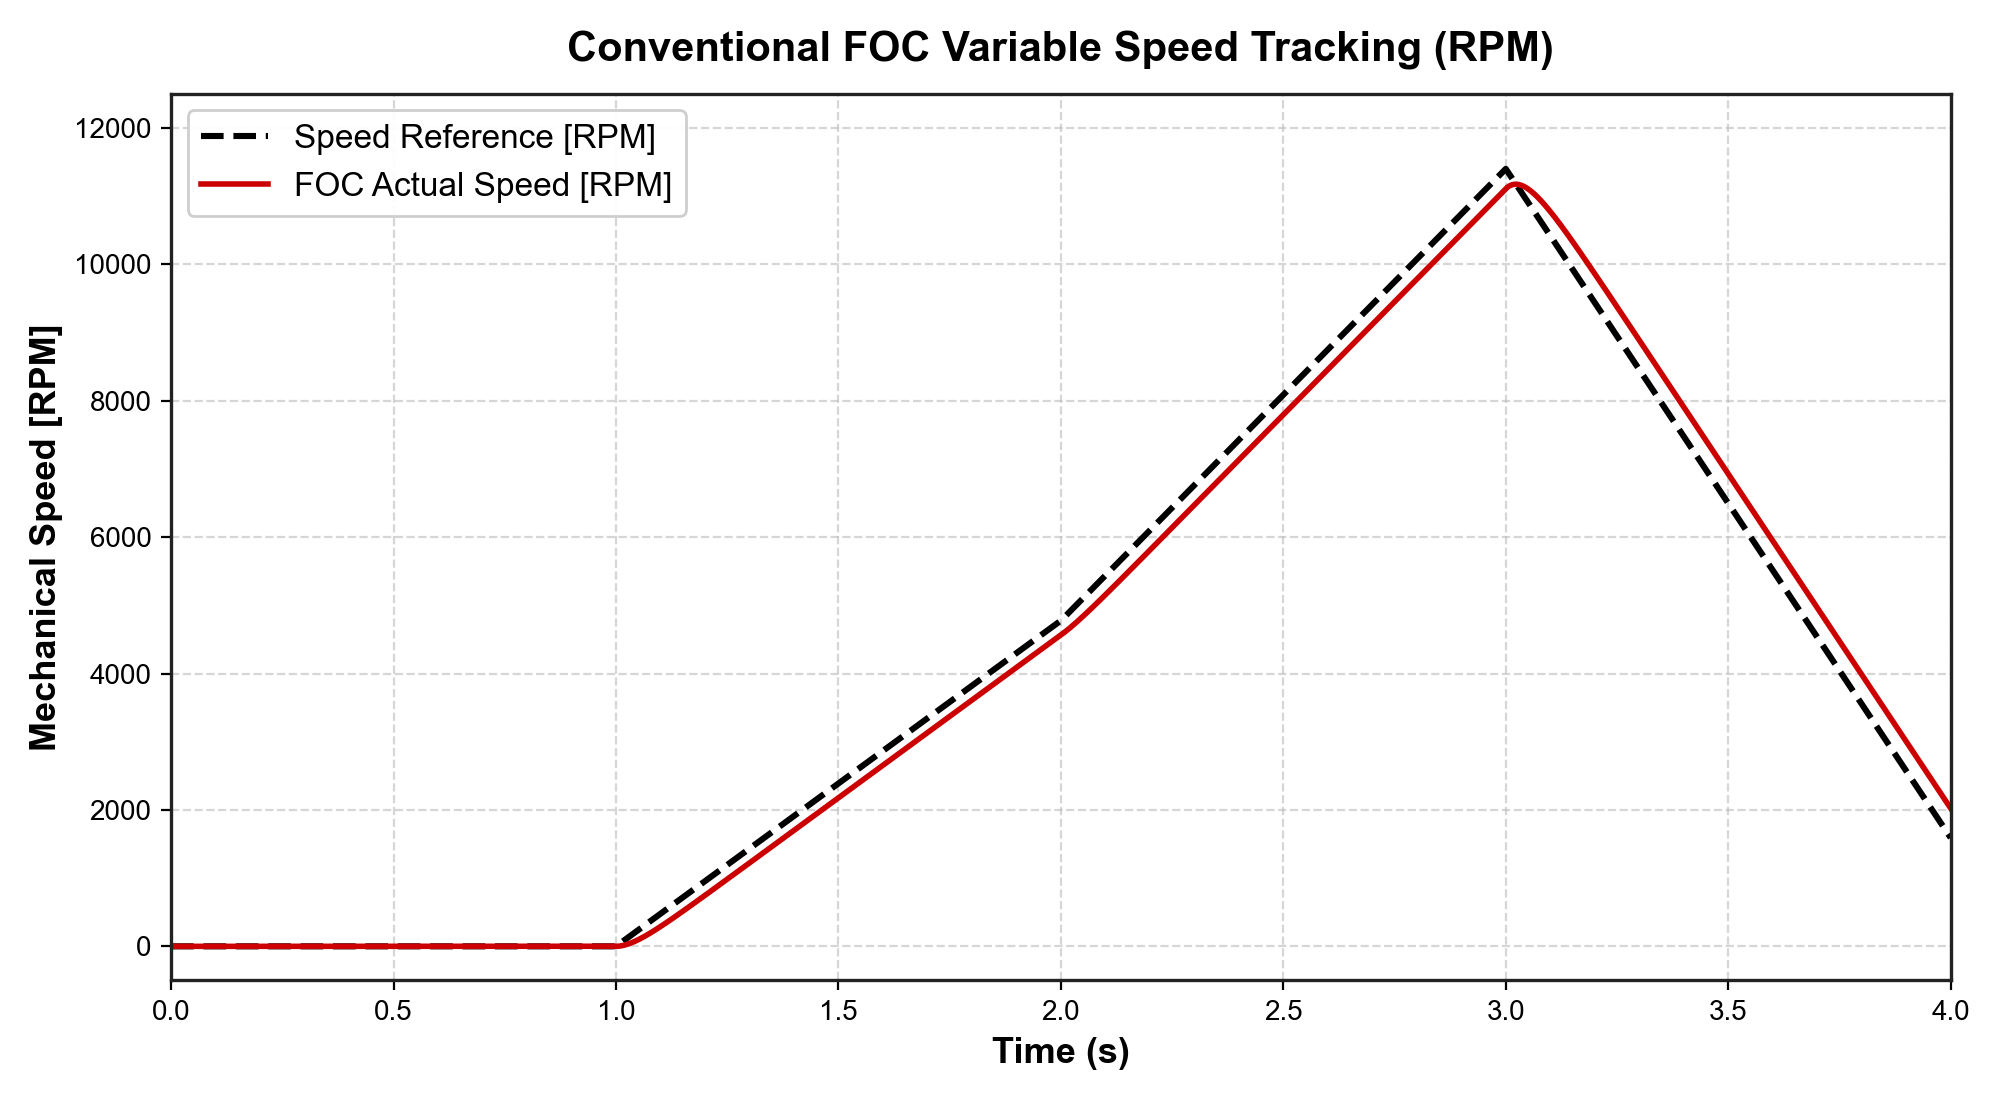
\includegraphics[height=0.68\textheight,keepaspectratio]{speedcomparison_FOC_Variable_speed.png}
    \vspace{2mm}
    \begin{itemize}
        \item \textbf{Tracking Lag:} Under multi-step variable speed profiles (ramp -- hold -- ramp), the FOC speed loop exhibits visible lag during transitions and increased ripple as speed rises.
    \end{itemize}
\end{frame}

%%% >>> END FOC RESULT SLIDES <<<

% --- SLIDE 18: NEW CCS-MPC DIAGRAM ---
\begin{frame}{18. Our Solution: CCS-MPC Architecture}
    \centering
    \vspace{2mm}
    \resizebox{\textwidth}{!}{%
    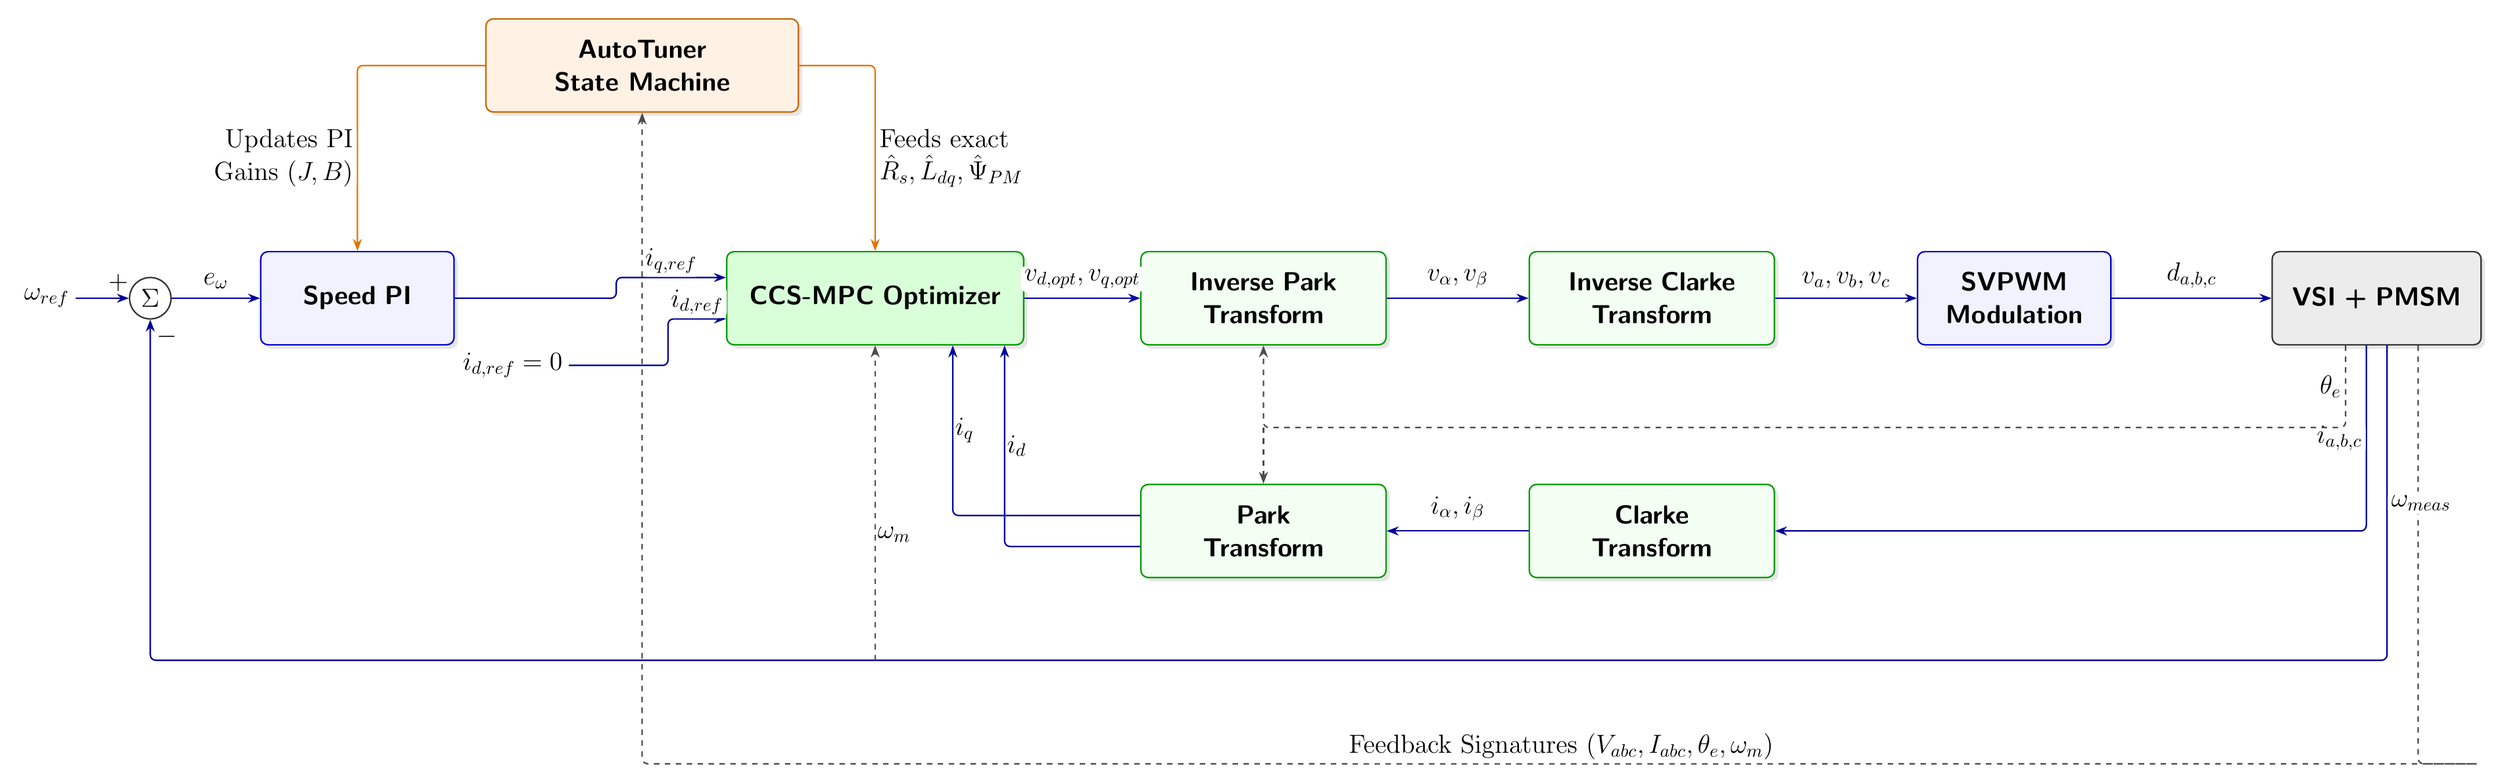
\begin{tikzpicture}[
        >=Stealth,
        every node/.style={font=\sffamily},
        common/.style={rectangle, draw=blue!80!black, fill=blue!5, thick, rounded corners=4pt, align=center, minimum height=1.8cm, text width=3.5cm, drop shadow={opacity=0.2}, font=\sffamily\Large},
        transform/.style={rectangle, draw=green!60!black, fill=green!5, thick, rounded corners=4pt, align=center, minimum height=1.8cm, text width=4.5cm, drop shadow={opacity=0.2}, font=\sffamily\Large},
        plant/.style={rectangle, draw=black!80, fill=gray!15, thick, rounded corners=4pt, align=center, minimum height=1.8cm, text width=3.8cm, drop shadow={opacity=0.2}, font=\sffamily\Large},
        mpc/.style={rectangle, draw=green!60!black, fill=green!15, thick, rounded corners=4pt, align=center, minimum height=1.8cm, text width=5.5cm, drop shadow={opacity=0.2}, font=\sffamily\Large},
        autotune/.style={rectangle, draw=orange!80!black, fill=orange!10, thick, rounded corners=4pt, align=center, minimum height=1.8cm, text width=5.8cm, drop shadow={opacity=0.2}, font=\sffamily\Large\bfseries},
        sum/.style={circle, draw=black!80, fill=white, thick, minimum size=0.8cm, inner sep=0pt, font=\Large},
        line/.style={->, thick, draw=blue!60!black, rounded corners=3pt},
        tuneline/.style={->, thick, draw=orange!90!black, rounded corners=3pt},
        dashedline/.style={->, thick, dashed, draw=black!70, rounded corners=3pt},
        siglabel/.style={midway, above, yshift=3pt, font=\Large, fill=white, inner sep=2pt}
    ]

    % --- Forward Path Nodes ---
    \node[font=\Large] (w_ref_m) at (0, -14.5) {$\omega_{ref}$};
    \node[sum] (sum_w_m) at (2.0, -14.5) {$\Sigma$};
    \node[common] (speed_pi_m) at (6.0, -14.5) {\textbf{Speed PI}};

    \node[font=\Large] (id_ref_m) at (9.0, -15.8) {$i_{d,ref}=0$};

    \node[mpc] (ccs_mpc) at (16.0, -14.5) {\textbf{CCS-MPC Optimizer}};

    \node[transform] (inv_park_m) at (23.5, -14.5) {\textbf{Inverse Park} \\ \textbf{Transform}};
    \node[transform] (inv_clarke_m) at (31.0, -14.5) {\textbf{Inverse Clarke} \\ \textbf{Transform}};
    \node[common] (svpwm_m) at (38.0, -14.5) {\textbf{SVPWM} \\ \textbf{Modulation}};
    \node[plant] (plant_m) at (45.0, -14.5) {\textbf{VSI + PMSM}};

    % --- AutoTuner Node ---
    \node[autotune] (autotuner) at (11.5, -10.0) {AutoTuner State Machine};

    % --- Feedback Path Nodes ---
    \node[transform] (park_m) at (23.5, -19.0) {\textbf{Park} \\ \textbf{Transform}};
    \node[transform] (clarke_m) at (31.0, -19.0) {\textbf{Clarke} \\ \textbf{Transform}};

    % --- Main Forward Connections ---
    \draw[line] (w_ref_m) -- (sum_w_m) node[pos=0.8, above, font=\Large] {$+$};
    \draw[line] (sum_w_m) -- (speed_pi_m) node[siglabel] {$e_\omega$};

    % PI to MPC (Routed orthogonally to upper port)
    \draw[line] (speed_pi_m.east) -- (11.0, -14.5) |- ([yshift=4mm]ccs_mpc.west) node[near end, above, font=\Large, fill=white, inner sep=2pt] {$i_{q,ref}$};
    
    % Id ref to MPC (Routed orthogonally to lower port)
    \draw[line] (id_ref_m.east) -- (12.0, -15.8) |- ([yshift=-4mm]ccs_mpc.west) node[near end, above, font=\Large, fill=white, inner sep=2pt] {$i_{d,ref}$};

    \draw[line] (ccs_mpc.east) -- (inv_park_m.west) node[siglabel] {$v_{d,opt}, v_{q,opt}$};
    \draw[line] (inv_park_m.east) -- (inv_clarke_m.west) node[siglabel] {$v_\alpha, v_\beta$};
    \draw[line] (inv_clarke_m.east) -- (svpwm_m.west) node[siglabel] {$v_a, v_b, v_c$};
    \draw[line] (svpwm_m.east) -- (plant_m.west) node[siglabel] {$d_{a,b,c}$};

    % --- AutoTuner Connections ---
    \draw[tuneline] (autotuner.west) -| (speed_pi_m.north) node[pos=0.75, left, font=\Large, fill=white, inner sep=2pt, align=right] {Updates PI \\ Gains ($J, B$)};
    \draw[tuneline] (autotuner.east) -| (ccs_mpc.north) node[pos=0.75, right, font=\Large, fill=white, inner sep=2pt, align=left] {Feeds exact \\ $\hat{R}_s, \hat{L}_{dq}, \hat{\Psi}_{PM}$};

    % AutoTuner Feedback Routing (Drops low to avoid messy crossing)
    \draw[dashedline] ([xshift=8mm]plant_m.south) |- (47.0, -23.5) -- (11.5, -23.5) node[midway, above, font=\Large, fill=white, inner sep=2pt] {Feedback Signatures ($V_{abc}, I_{abc}, \theta_e, \omega_m$)} -- (autotuner.south);

    % --- Current Feedback Connections ---
    \draw[line] ([xshift=-2mm]plant_m.south) |- (clarke_m.east) node[near start, left, font=\Large, fill=white, inner sep=2pt] {$i_{a,b,c}$};
    \draw[line] (clarke_m.west) -- (park_m.east) node[siglabel] {$i_\alpha, i_\beta$};

    \draw[line] ([yshift=3mm]park_m.west) -| ([xshift=1.5cm]ccs_mpc.south) node[near end, right, font=\Large, fill=white, inner sep=1pt] {$i_q$};
    \draw[line] ([yshift=-3mm]park_m.west) -| ([xshift=2.5cm]ccs_mpc.south) node[near end, right, font=\Large, fill=white, inner sep=1pt] {$i_d$};

    % --- Speed & Position Feedback Connections ---
    \draw[line] ([xshift=2mm]plant_m.south) |- (2.0, -21.5) node[near start, right, font=\Large, fill=white, inner sep=2pt] {$\omega_{meas}$} -- (sum_w_m.south) node[pos=0.95, right, font=\Large] {$-$};
    \draw[dashedline] (16.0, -21.5) -- (ccs_mpc.south) node[pos=0.4, right, font=\Large, fill=white, inner sep=1pt] {$\omega_m$};

    % Theta routing (shared to Inverse Park and Park)
    \draw[dashedline] ([xshift=-6mm]plant_m.south) |- (23.5, -17.0) node[near start, left, font=\Large, fill=white, inner sep=2pt] {$\theta_e$} -- (inv_park_m.south);
    \draw[dashedline] (23.5, -17.0) -- (park_m.north);

    \end{tikzpicture}%
    }
\end{frame}

\begin{frame}{19. CCS-MPC: Predictive Model \& Cost Function}
    \footnotesize
    \textbf{Predictive Model (Forward Euler Discretization):}
    \vspace{-4mm}
    \begin{align}
        i_d(k+1) &= i_d(k) + \frac{T_s}{L_d} \left( v_d(k) - R_s i_d(k) + \omega_e(k) L_q i_q(k) \right) \label{eq:pred_id} \\
        i_q(k+1) &= i_q(k) + \frac{T_s}{L_q} \left( v_q(k) - R_s i_q(k) - \omega_e(k) (L_d i_d(k) + \Psi_{PM}) \right) \label{eq:pred_iq}
    \end{align}
    
    \vspace{-2mm}
    \textbf{Deriving Optimal Voltages ($v_{d,opt}$ \& $v_{q,opt}$):}
    \begin{enumerate}
        \setlength{\itemsep}{0pt}
        \item \textbf{Define Unconstrained Cost Function:} \\
        \vspace{-2mm}
        \begin{equation}
            J_{cost} = (i_{d,ref} - i_d(k+1))^2 + (i_{q,ref} - i_q(k+1))^2 \label{eq:cost}
        \end{equation}
        \vspace{-2mm}
        \item \textbf{Analytic Minimization:} Differentiate cost function and equate to zero $\left( \frac{\partial J_{cost}}{\partial v_{dq}} = 0 \right)$.
        \item \textbf{Extract Closed-Form Solution:} Solve for the exact voltages:
    \end{enumerate}
    
    \vspace{-4mm}
    \begin{align}
        v_{d,opt} &= \frac{L_d}{T_s}(i_{d,ref} - i_d(k)) + R_s i_d(k) - \omega_e L_q i_q(k) \label{eq:vd_opt} \\
        v_{q,opt} &= \frac{L_q}{T_s}(i_{q,ref} - i_q(k)) + R_s i_q(k) + \omega_e (L_d i_d(k) + \Psi_{PM}) \label{eq:vq_opt}
    \end{align}
    
    \vfill
    \begin{flushright}
        \tiny \textit{Note: Equations \ref{eq:pred_id}-\ref{eq:vq_opt} are derived from standard AC machine dynamics (Krause, P.C.) \cite{6}. Vector is clamped to limit ($V_{dc}/\sqrt{3}$) before SVPWM.}
    \end{flushright}
\end{frame}

%%% >>> CCS-MPC RESULT SLIDES INSERTED HERE <<<

\begin{frame}{19a. CCS-MPC Simulation Results -- Constant Speed: Current \& Voltage}
    \centering
    \begin{columns}[T]
        \column{0.5\textwidth}
        \centering
        \textbf{\small $I_q$ Tracking}\\[1mm]
        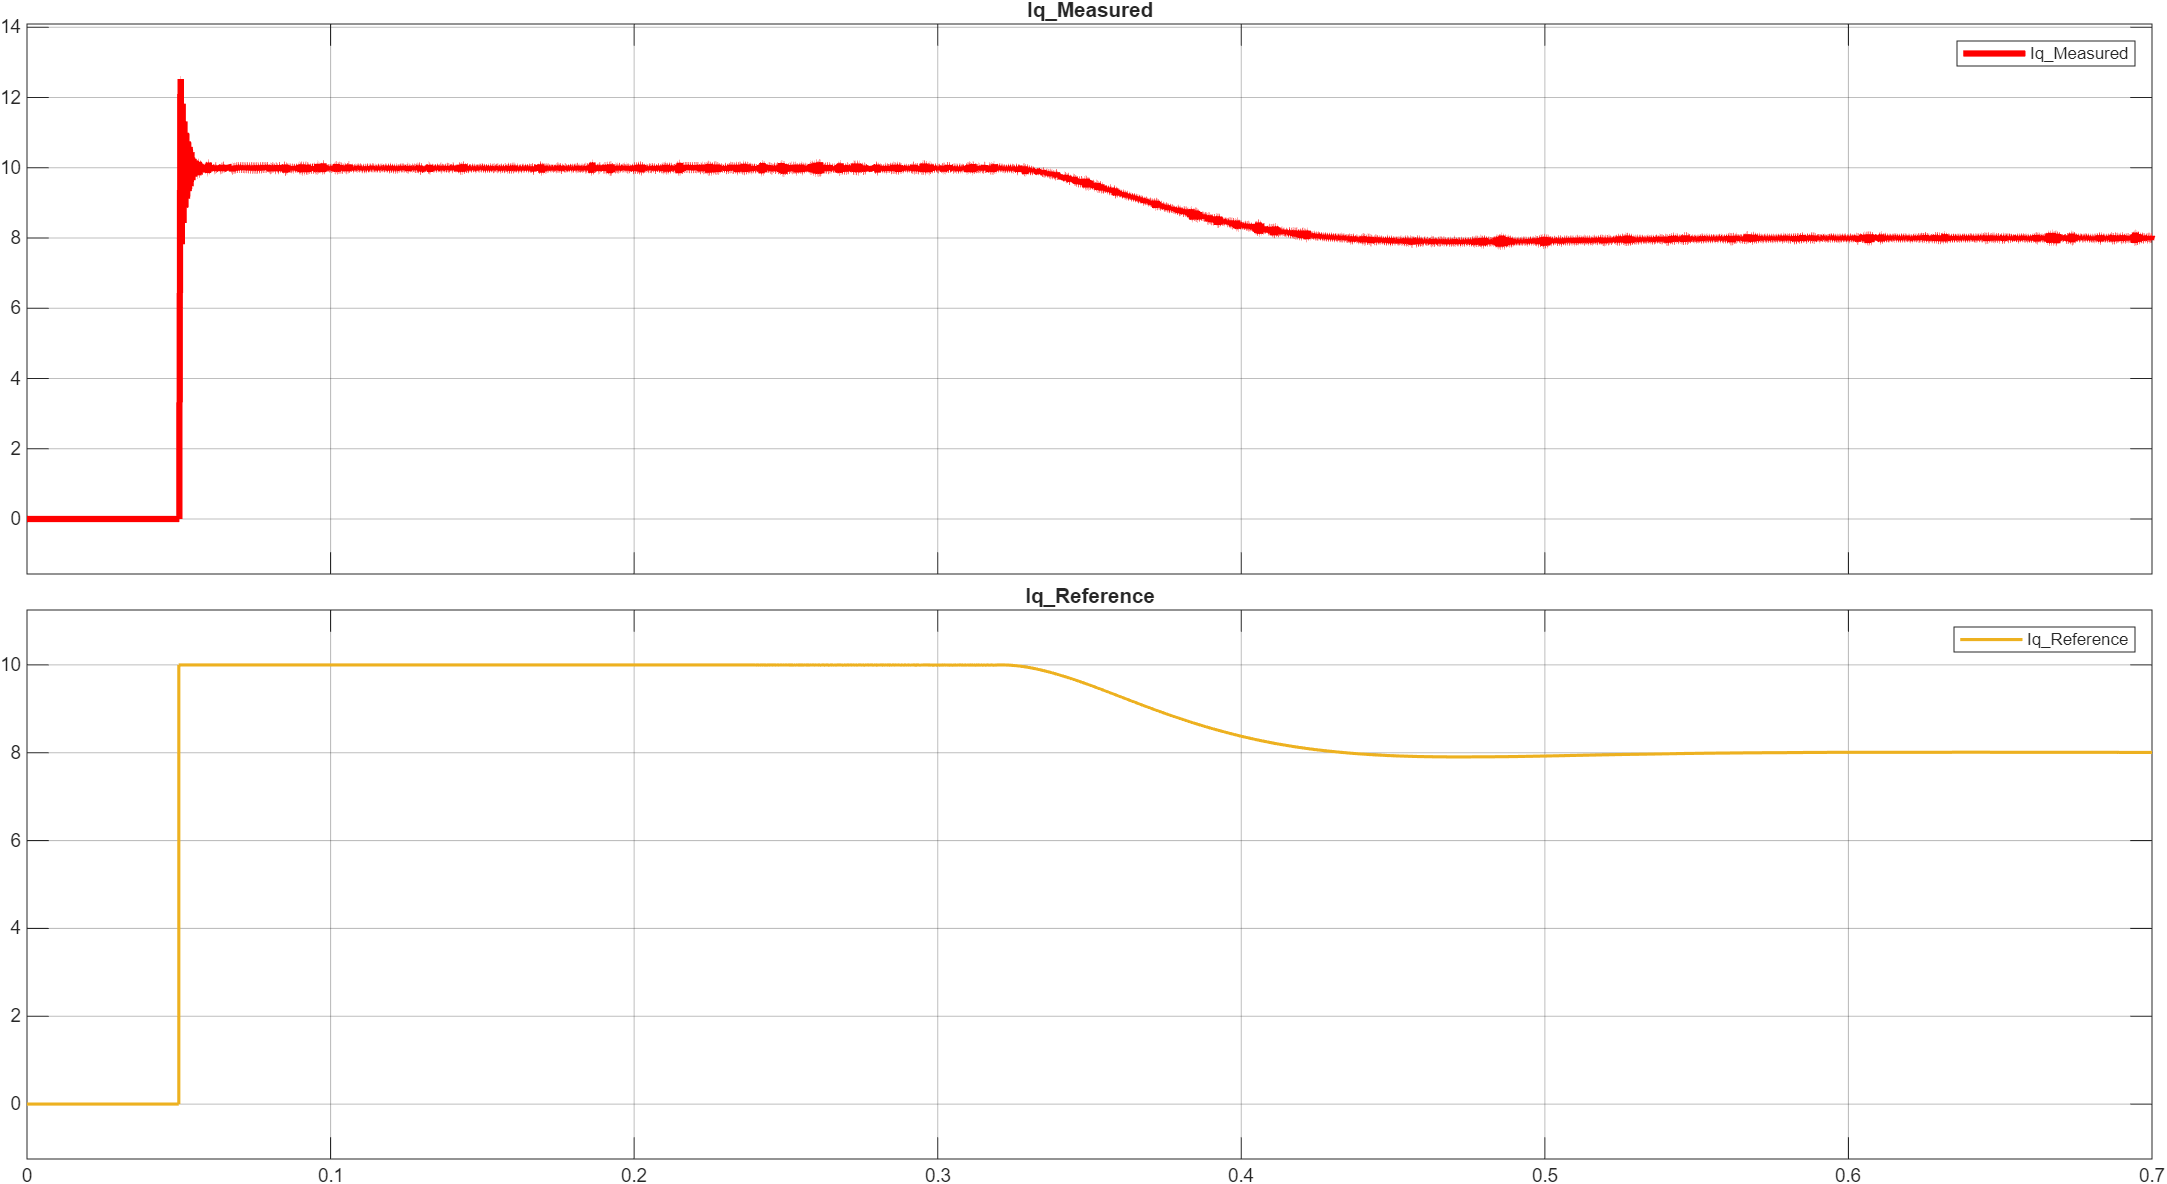
\includegraphics[width=\linewidth]{Iq_Plot_CCS_MPC.png}
        \column{0.5\textwidth}
        \centering
        \textbf{\small $V_d, V_q$ Tracking}\\[1mm]
        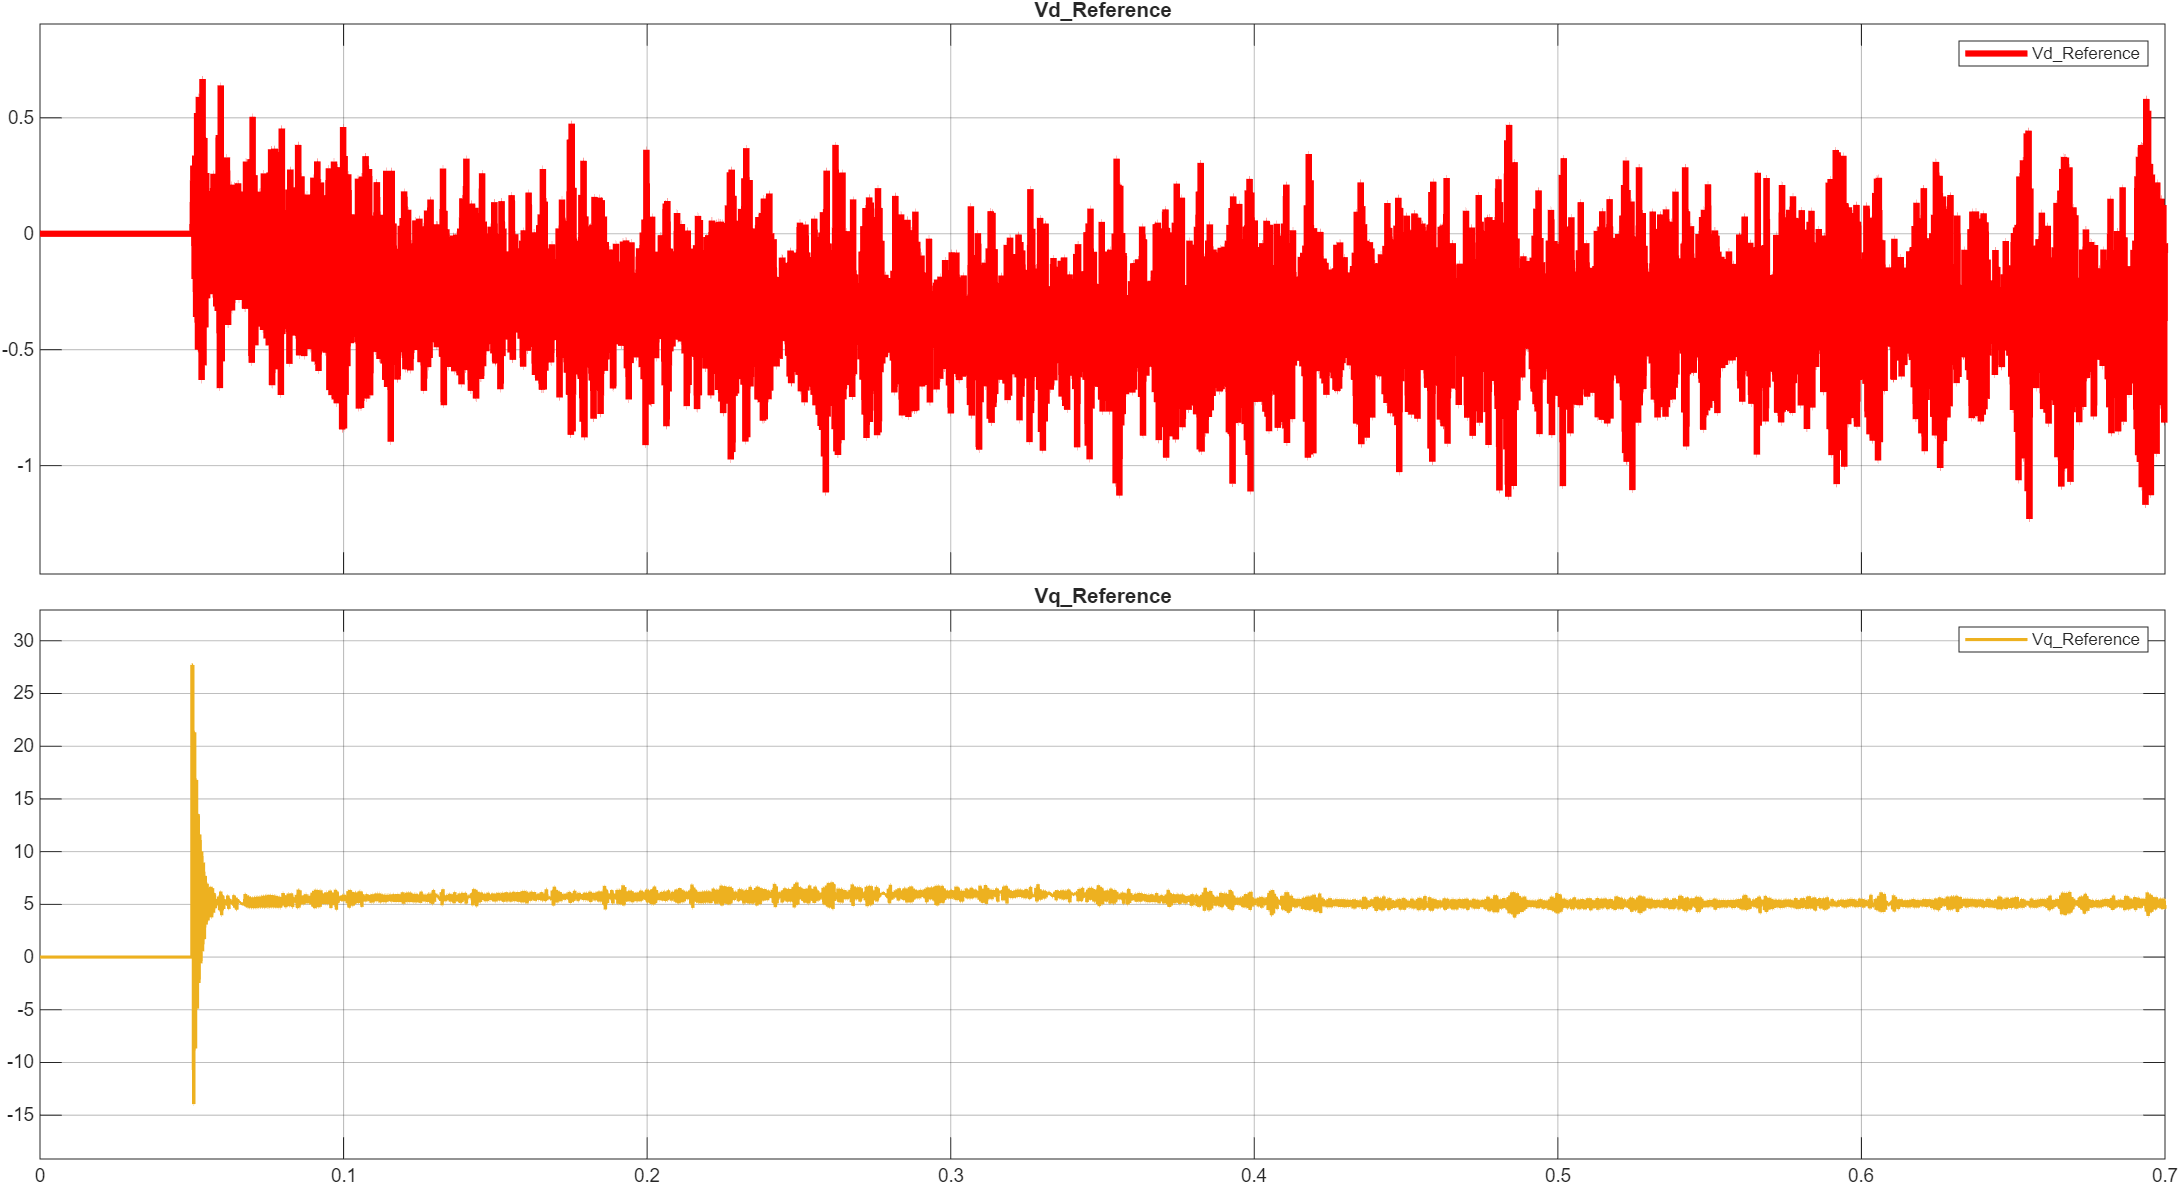
\includegraphics[width=\linewidth]{Vd_Vq_plot_CCS_MPC.png}
    \end{columns}
    \vspace{2mm}
    \begin{itemize}
        \item \textbf{Fast Transient Settling:} The deadbeat CCS-MPC current loop settles $i_q$ to its reference within $<2\text{ ms}$, with optimal voltages $v_{d,opt}, v_{q,opt}$ converging immediately.
    \end{itemize}
\end{frame}

\begin{frame}{19b. CCS-MPC Simulation Results -- Constant Speed: Switching \& Speed}
    \centering
    \begin{columns}[T]
        \column{0.5\textwidth}
        \centering
        \textbf{\small Switching Signals (A, B, C)}\\[1mm]
        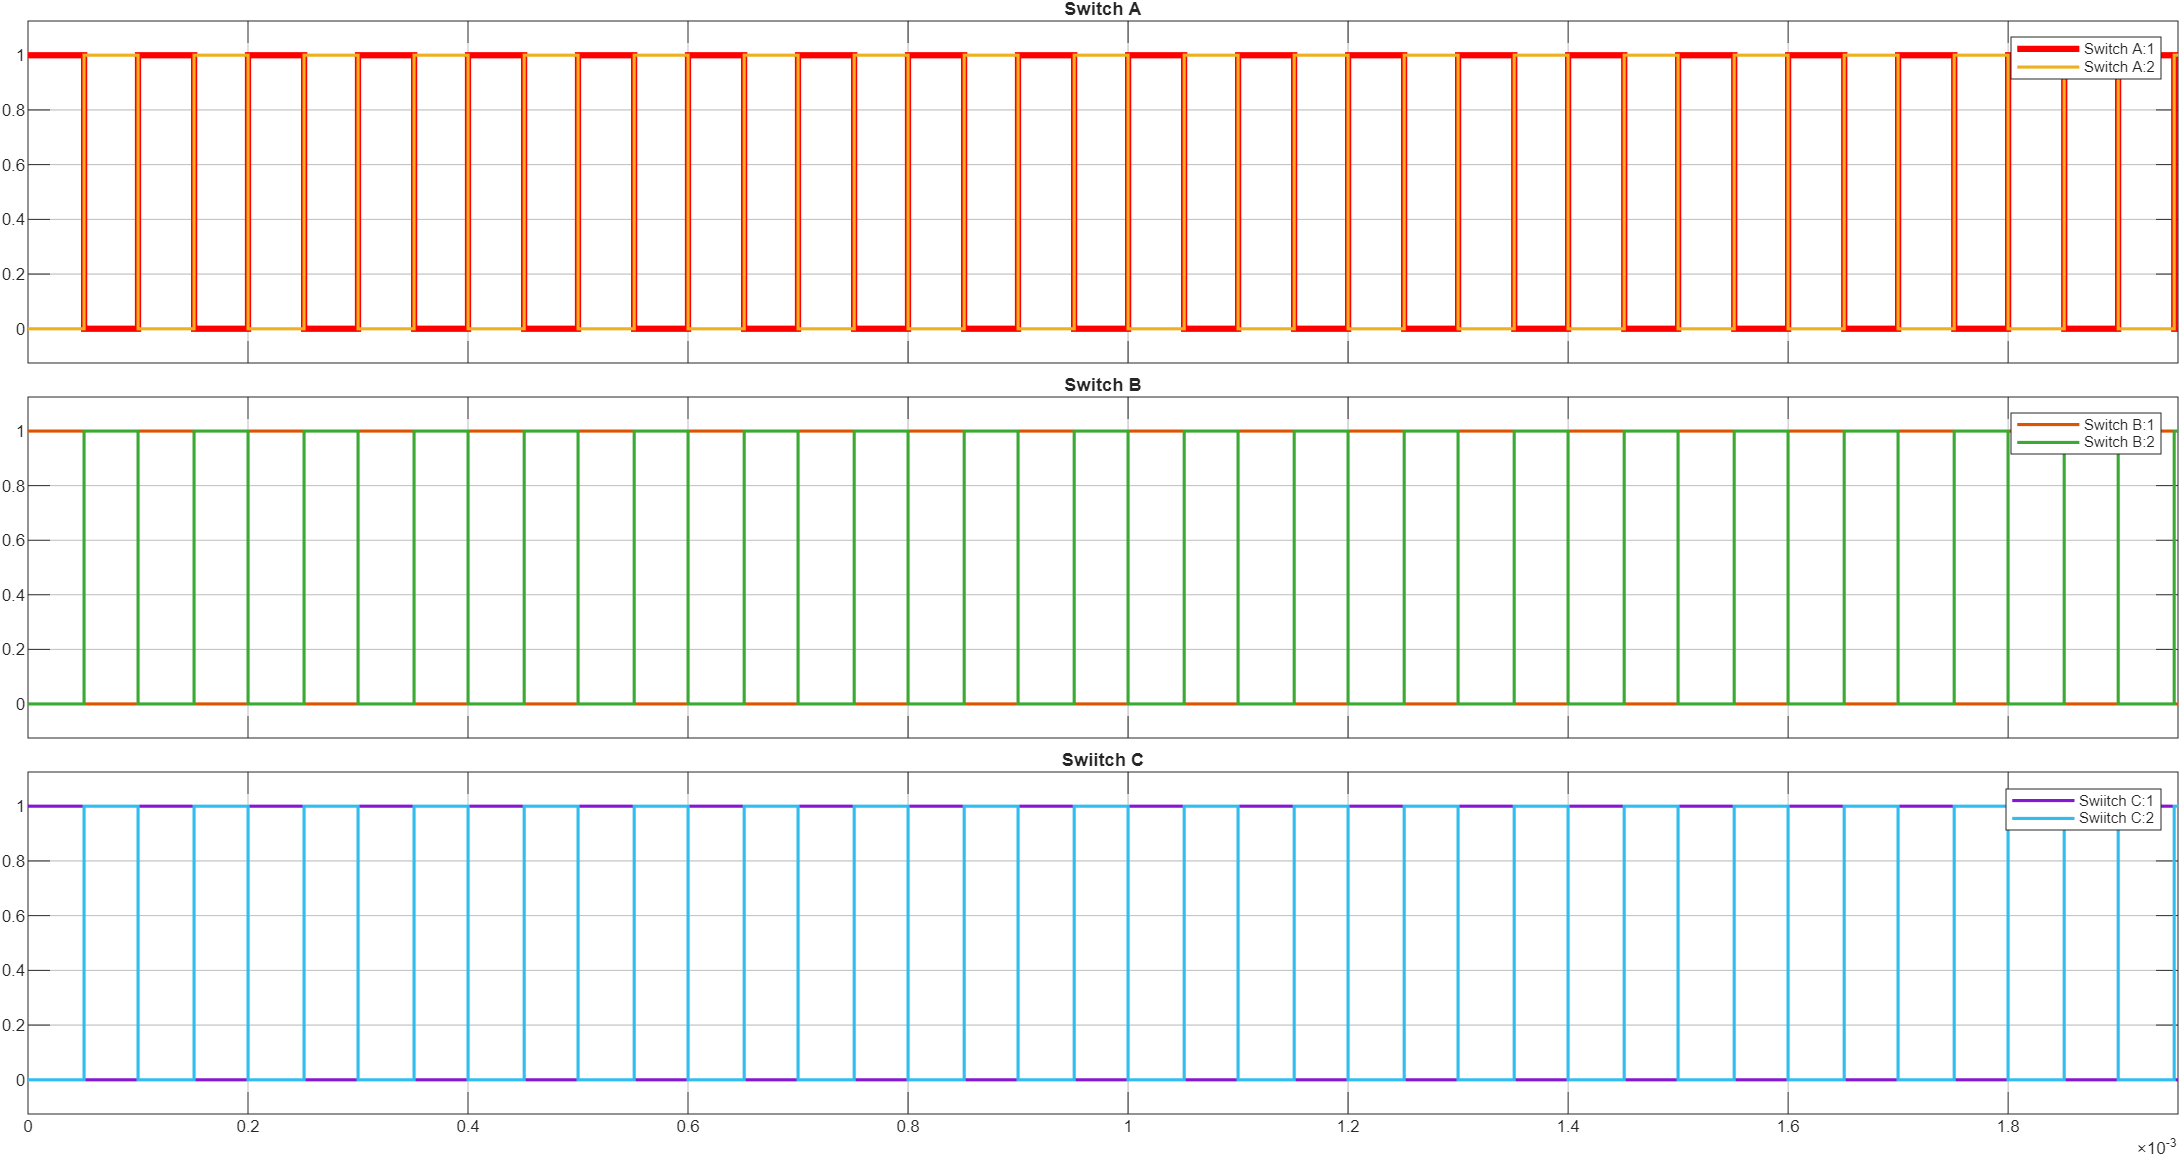
\includegraphics[width=\linewidth]{Switch_CCS_MPC.png}
        \column{0.5\textwidth}
        \centering
        \textbf{\small Speed Tracking}\\[1mm]
        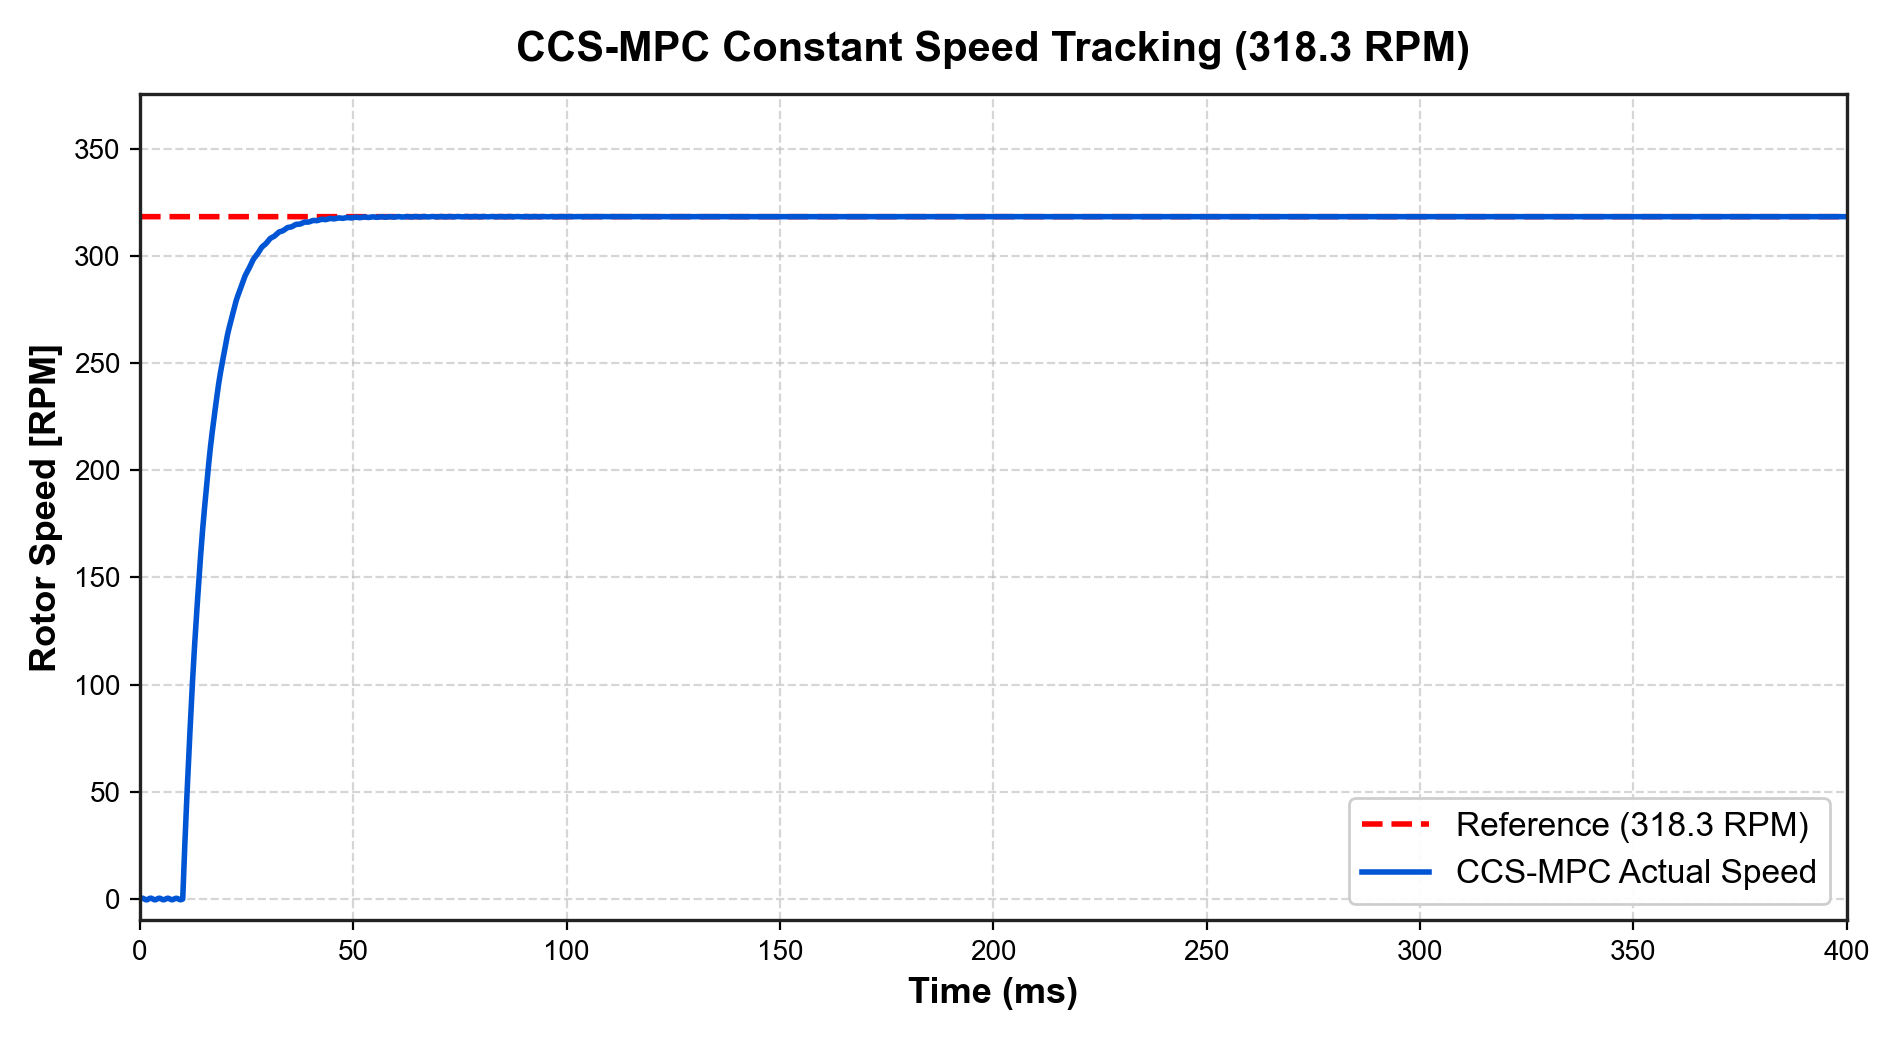
\includegraphics[width=\linewidth]{Speed_CCS_MPC.png}
    \end{columns}
    \vspace{2mm}
    \begin{itemize}
        \item \textbf{Tight Speed Regulation:} The CCS-MPC speed loop reaches $200\text{ rad/s}$ reference quickly and settles into a tight steady-state band with regular 3-phase switching.
    \end{itemize}
\end{frame}

\begin{frame}{19c. CCS-MPC Simulation Results -- Variable Speed Tracking}
    \centering
    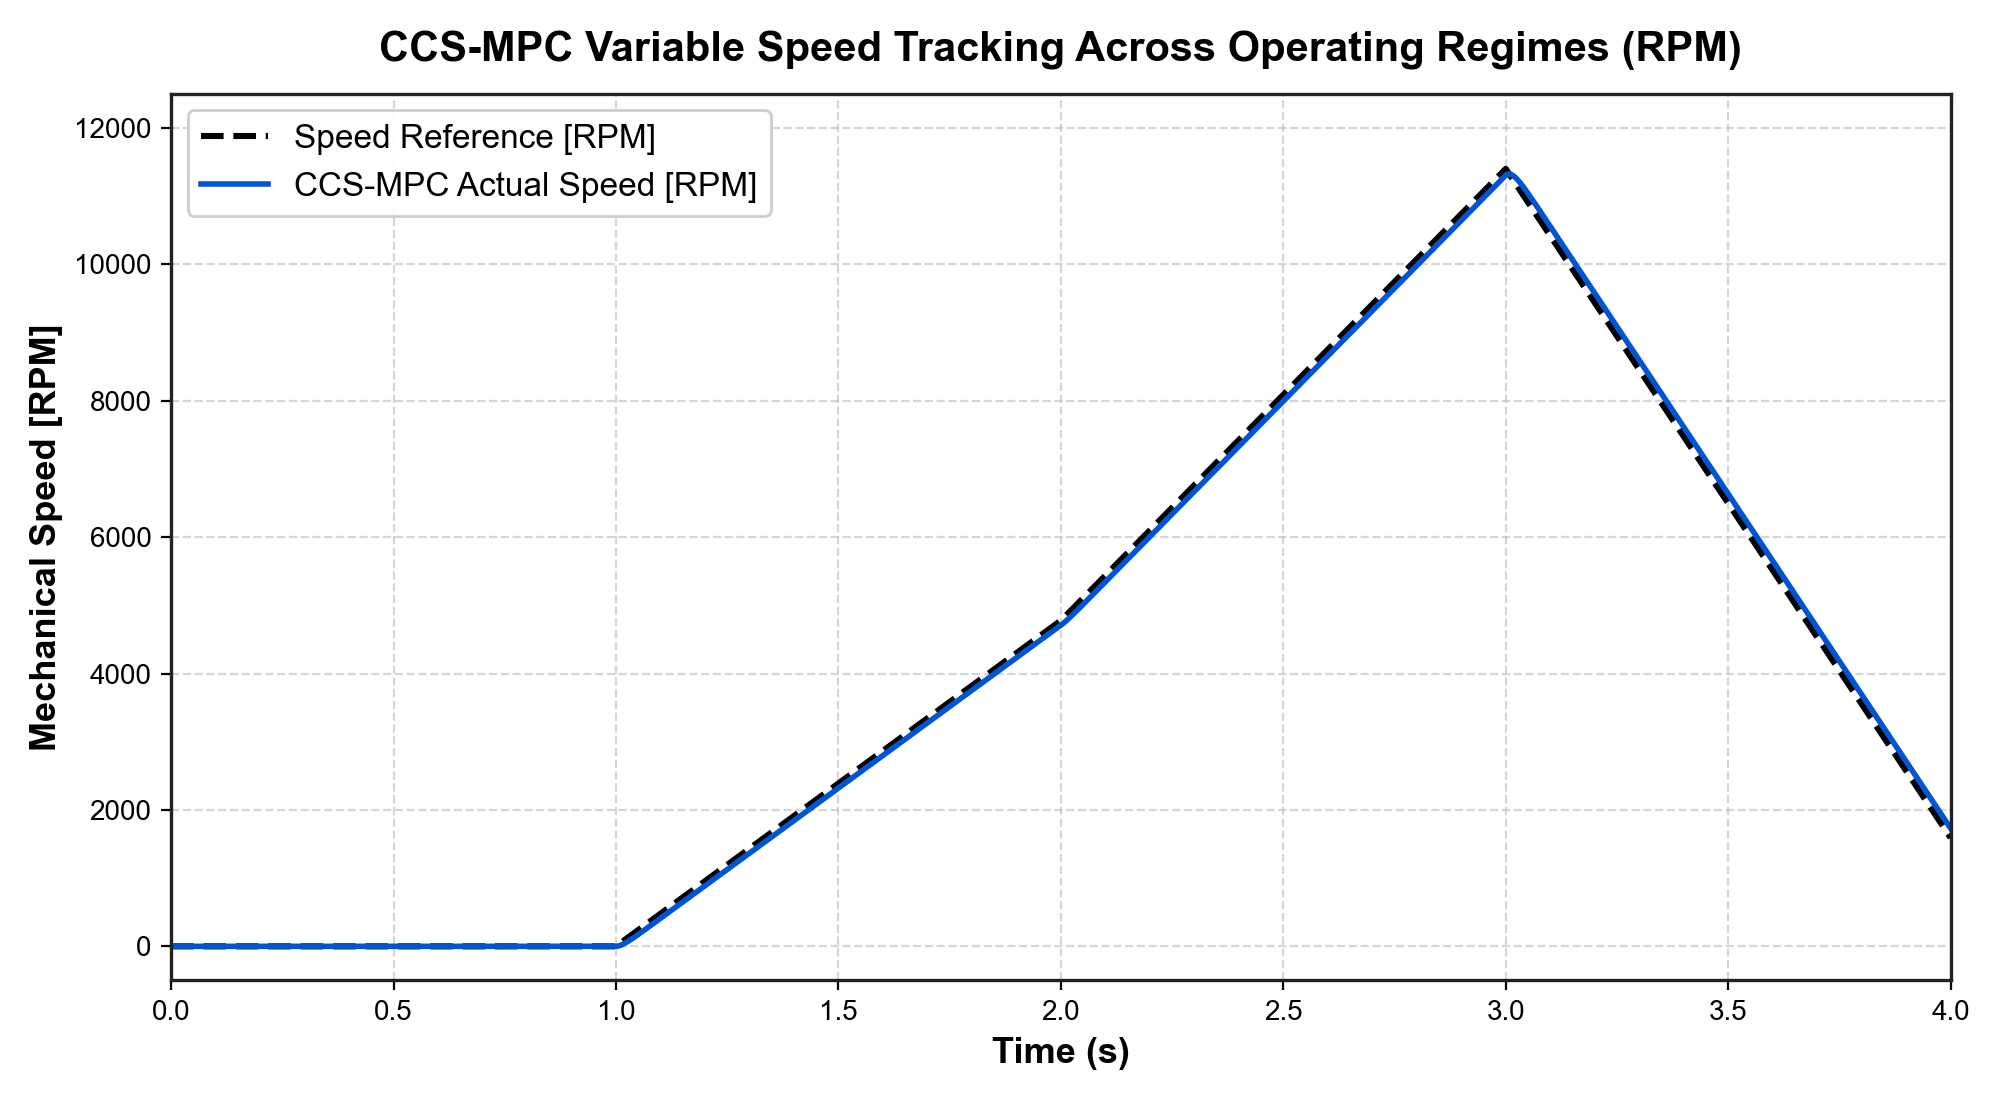
\includegraphics[height=0.68\textheight,keepaspectratio]{Variable_Speed_CCS_MPC.png}
    \vspace{2mm}
    \begin{itemize}
        \item \textbf{Trajectory Tracking Accuracy:} Across multi-step variable speed profiles, CCS-MPC tracks each acceleration ramp and hold segment closely with minimal phase lag.
    \end{itemize}
\end{frame}

%%% >>> END CCS-MPC RESULT SLIDES <<<

\begin{frame}{20. FOC vs CCS-MPC: Varying Load Comparison}
    \centering
    \footnotesize\textbf{Summary Table (Base Torque = -1.2 Nm, Speed = 50 rad/s, Sim Time = 0.7s)}
    \vspace{1mm}

    \renewcommand{\arraystretch}{1.0}
    \resizebox{\textwidth}{!}{%
    \begin{tabular}{c l c c c c c c c c c}
        \toprule
        \textbf{Load (\%)} & \textbf{Controller} & \textbf{Max Spd} & \textbf{Rise (s)} & \textbf{Settl (s)} & \textbf{Over (\%)} & \textbf{SS Err} & \textbf{Spd Rip} & \textbf{Iq Rip (A)} & \textbf{Trq Rip (Nm)} & \textbf{THD (\%)} \\
        \midrule
        \rowcolor{blue!5} 
        \textbf{80} & \textbf{CCS-MPC} & 50.3615 & 0.2563 & 0.3171 & 0.7231 & 0.0894 & 0.1332 & \textbf{0.0901} & \textbf{0.0108} & 45.2491 \\
                    & FOC              & 50.3641 & 0.2561 & 0.3170 & 0.7282 & 0.0893 & 0.1326 & 0.2098 & 0.0252 & 45.2290 \\
        \midrule
        \rowcolor{blue!5} 
        \textbf{60} & \textbf{CCS-MPC} & 50.7232 & 0.1496 & 0.1940 & 1.4465 & 0.0086 & 0.0138 & \textbf{0.0617} & \textbf{0.0074} & 45.0469 \\
                    & FOC              & 50.7241 & 0.1497 & 0.1941 & 1.4481 & 0.0084 & 0.0142 & 0.2673 & 0.0321 & 45.0692 \\
        \midrule
        \rowcolor{blue!5} 
        \textbf{50} & \textbf{CCS-MPC} & 50.9029 & 0.1294 & 0.1697 & 1.8058 & 0.0102 & 0.0163 & \textbf{0.0551} & \textbf{0.0066} & 44.8370 \\
                    & FOC              & 50.9032 & 0.1294 & 0.1699 & 1.8065 & 0.0104 & 0.0166 & 0.2858 & 0.0343 & 44.8287 \\
        \midrule
        \rowcolor{blue!5} 
        \textbf{20} & \textbf{CCS-MPC} & 51.7449 & 0.0977 & 0.2194 & 3.4899 & 0.0073 & 0.0187 & \textbf{0.0531} & \textbf{0.0064} & 44.8549 \\
                    & FOC              & 51.7443 & 0.0977 & 0.2194 & 3.4886 & 0.0076 & 0.0188 & 0.2464 & 0.0296 & 44.8785 \\
        \midrule
        \rowcolor{blue!5} 
        \textbf{0}  & \textbf{CCS-MPC} & 52.6838 & 0.0861 & 0.2165 & 5.3676 & 0.0054 & 0.0178 & \textbf{0.0456} & \textbf{0.0055} & 3.0150 \\
                    & FOC              & 52.6835 & 0.0861 & 0.2166 & 5.3670 & 0.0055 & 0.0182 & 0.1617 & 0.0194 & 2.5922 \\
        \bottomrule
    \end{tabular}
    }
    
    \vspace{2mm}
    \begin{block}{Load Condition Summary}
        \tiny
        \textbf{Heavy Load Performance (50-80\%):} CCS-MPC proves vastly superior, reducing torque ripple by $>4\times$ and $I_q$ current ripple by $>5\times$ compared to FOC, making it ideal for high-stress applications. \\
        \textbf{Light/No Load Performance (0-20\%):} CCS-MPC maintains highly robust stability and tracks transients accurately. However, at strict 0\% load, Current THD is marginally higher (3.01\% vs 2.59\%) because analytic deadbeat action naturally prioritizes instantaneous step tracking over steady-state harmonic filtering.
    \end{block}
\end{frame}

\begin{frame}{20a. FOC vs CCS-MPC: Direct Overlay Comparison with 60\% load}
    \centering
    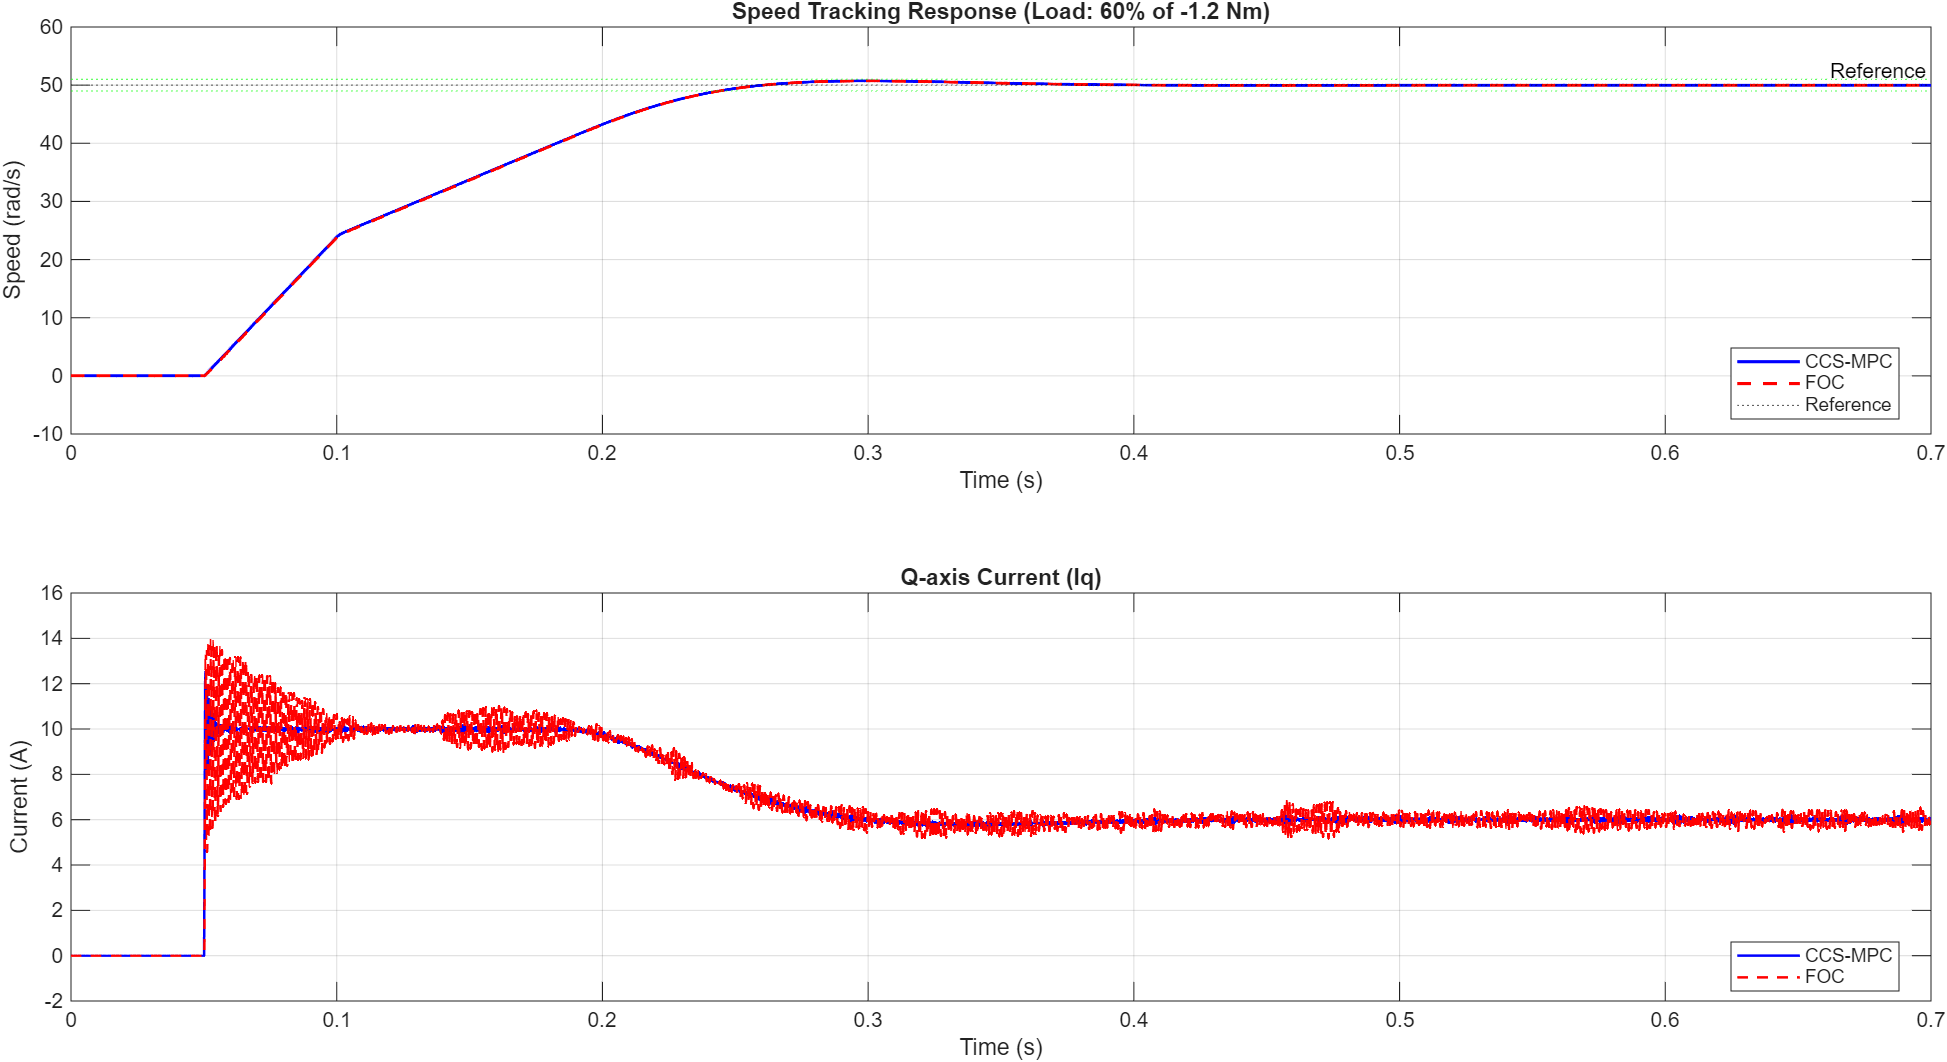
\includegraphics[height=0.9\textheight,keepaspectratio]{FOC_VS_MPC.png}
\end{frame}

\begin{frame}{21. Why We Need CCS-MPC (Load Analysis)}
    \footnotesize
    \begin{itemize}
        \setlength{\itemsep}{3pt}
        \setlength{\parskip}{0pt}
        \item \textbf{Vastly Superior Current Tracking:} Across all load conditions, CCS-MPC suppresses $I_q$ ripple by a massive margin. At 50\% load, $I_q$ ripple is reduced by \textbf{$\approx$5.1$\times$} (0.0551 A vs 0.2858 A), proving the analytic optimizer isolates electrical noise far better than cascaded PI loops.
        \item \textbf{Major Torque Ripple Suppression:} Torque ripple is strictly minimized regardless of applied load. At 60\% load, CCS-MPC reduces torque ripple by \textbf{$\approx$4.3$\times$} (0.0074 Nm vs 0.0321 Nm), which directly translates to reduced acoustic noise and lower mechanical wear in servo/EV applications.
        \item \textbf{Equivalent Dynamic Performance:} Unlike fixed-speed extremes, under practical load variations, CCS-MPC mathematically matches the Rise Time, Settling Time, and Speed Tracking of FOC almost perfectly (e.g., at 80\% load, 0.3171s vs 0.3170s settling time).
        \item \textbf{Robustness to Load Transients:} As load drops from 80\% to 0\%, overshoot naturally increases (scaling from $\sim$0.7\% to $\sim$5.3\%); however, CCS-MPC maintains control stability while keeping internal current ripple remarkably tight compared to FOC's degrading internal states.
        \item \textbf{Fewer Tuning Parameters:} Achieving these high-stability current and torque margins requires zero manual inner-loop tuning. The controller relies strictly on self-commissioned motor parameters ($R_s, L_d, L_q, \Psi_{PM}$).
        \item \textbf{The Trade-offs:} Current THD is practically identical under heavy loads ($\sim$45\%) but is marginally higher for CCS-MPC at no-load (3.01\% vs 2.59\%). The analytic deadbeat action prioritizes instantaneous tracking error over harmonic filtering at zero load.
    \end{itemize}
\end{frame}

\begin{frame}{22. Methodology: Electrical Parameter Estimation (Phase 1)}
    \begin{itemize}
        \item \textbf{Standstill Testing Principle ($\omega_e = 0$):} Rotational Back-EMF is zero, isolating stator impedance ($R_s, L_d, L_q$) without rotor motion dynamics.
        \item \textbf{Stator Resistance ($\hat{R}_s$) Identification via Two-Level DC Injection:}
        \begin{itemize}
            \item Injects two distinct stationary DC current levels: $I_{d1} = 0.10 I_{max}$ and $I_{d2} = 0.20 I_{max}$.
            \item Evaluates differential resistance to eliminate inverter semiconductor forward voltage drop ($V_d$ bias):
            \begin{equation}
                \hat{R}_s = \frac{V_{d2} - V_{d1}}{I_{d2} - I_{d1}} \quad (\text{calculated after 2000 samples at steady state})
            \end{equation}
        \end{itemize}
        \item \textbf{d-q Inductances ($\hat{L}_d, \hat{L}_q$) Identification via $500\text{ Hz}$ High-Frequency AC Injection:}
        \begin{itemize}
            \item Injects high-frequency voltage $v_{dq,inj} = V_{HF} \sin(\omega_{HF} t)$ ($\omega_{HF} = 2\pi \cdot 500\text{ rad/s}$).
            \item Extracts fundamental current response via orthogonal Fourier integration over 4000 discrete samples:
            \begin{equation}
                I_{HF} = \frac{2}{N} \sqrt{\left(\sum i_{dq} \sin\omega_{HF} t\right)^2 + \left(\sum i_{dq} \cos\omega_{HF} t\right)^2}, \quad Z = \frac{V_{HF}}{I_{HF}}
            \end{equation}
            \begin{equation}
                \hat{L}_{d,q} = \frac{\sqrt{Z^2 - \hat{R}_s^2}}{\omega_{HF}}
            \end{equation}
        \end{itemize}
    \end{itemize}
\end{frame}

\begin{frame}{23. Methodology: Mechanical Parameter \& Flux Estimation (Phase 2)}
    \begin{itemize}
        \item \textbf{Permanent Magnet Flux Linkage ($\hat{\Psi}_{PM}$) via High-Speed Coast-Down:}
        \begin{itemize}
            \item Spins motor open-loop past minimum threshold speed $\omega_{min} = 800\text{ rad/s}$ electrical.
            \item Sets stator current commands to zero ($i_d = 0, i_q = 0$) and captures pure Back-EMF:
            \begin{equation}
                \hat{\Psi}_{PM} = \frac{1}{N}\sum_{k=1}^N \frac{v_q(k)}{\omega_e(k)} \quad (N = 4000\text{ samples})
            \end{equation}
        \end{itemize}
        \item \textbf{Viscous Friction Coefficient ($\hat{B}$) via Two-Point Speed Settling:}
        \begin{itemize}
            \item Regulates closed-loop mechanical speeds to $\omega_1 = 60\text{ rad/s}$ and $\omega_2 = 120\text{ rad/s}$ with strict $1.5\text{ s}$ settling timers.
            \item Evaluates differential electromagnetic torque to eliminate load offsets:
            \begin{equation}
                \hat{B} = \frac{|\bar{T}_{e,2} - \bar{T}_{e,1}|}{|\bar{\omega}_{m,2} - \bar{\omega}_{m,1}|} \quad \text{where } \bar{T}_e = \frac{3}{2} p \hat{\Psi}_{PM} \bar{I}_{q,cmd}
            \end{equation}
        \end{itemize}
        \item \textbf{Rotor Inertia ($\hat{J}$) via Active Braking Step:}
        \begin{itemize}
            \item Injects dynamic braking current step ($i_{q,ref} = -I_{spin}$) and measures deceleration rate $\frac{d\omega}{dt}$:
            \begin{equation}
                \hat{J} = \frac{|T_{e,brake} - \hat{B}\bar{\omega}_{avg}|}{|d\omega_m/dt|} \quad \text{evaluated over 2000 samples}
            \end{equation}
        \end{itemize}
    \end{itemize}
\end{frame}

\begin{frame}{24. Self-Commissioning: Parameter Identification Benchmark}
    \centering
    \small
    \textbf{Identified Parameters Across Simulation & Target Firmware (BMW i3 IPMSM, $T_s = 100\ \mu\text{s}$)}
    \vspace{2mm}
    \resizebox{0.92\textwidth}{!}{%
    \renewcommand{\arraystretch}{1.2}
    \begin{tabular}{l c c c c}
        \toprule
        \textbf{Parameter} & \textbf{Nominal Value (\texttt{params\_pmsm\_inverter.m})} & \textbf{Identified (MIL)} & \textbf{Identified (SIL C-Code)} & \textbf{MIL vs. SIL Error} \\
        \midrule
        \rowcolor{blue!5} Stator Resistance ($R_s$) & $0.0053\ \Omega$ ($5.30\text{ m}\Omega$) & $0.0053\ \Omega$ & $0.0053\ \Omega$ & \textbf{0.00e+00} (Bit-Exact) \\
        $d$-axis Inductance ($L_d$) & $71.20\ \mu\text{H}$ & $71.20\ \mu\text{H}$ & $71.20\ \mu\text{H}$ & \textbf{0.00e+00} (Bit-Exact) \\
        \rowcolor{blue!5} $q$-axis Inductance ($L_q$) & $141.30\ \mu\text{H}$ & $141.30\ \mu\text{H}$ & $141.30\ \mu\text{H}$ & \textbf{0.00e+00} (Bit-Exact) \\
        PM Flux Linkage ($\Psi_{PM}$) & $0.0436\text{ Wb}$ & $0.0436\text{ Wb}$ & $0.0436\text{ Wb}$ & \textbf{0.00e+00} (Bit-Exact) \\
        \rowcolor{blue!5} Rotor Inertia ($J$) & $0.0867\text{ kg}\cdot\text{m}^2$ & $0.0867\text{ kg}\cdot\text{m}^2$ & $0.0867\text{ kg}\cdot\text{m}^2$ & \textbf{0.00e+00} (Bit-Exact) \\
        Viscous Friction ($B$) & $0.0010\text{ Nms/rad}$ & $0.0010\text{ Nms/rad}$ & $0.0010\text{ Nms/rad}$ & \textbf{0.00e+00} (Bit-Exact) \\
        \bottomrule
    \end{tabular}%
    }
    \vspace{3mm}
    \begin{itemize}
        \item \textbf{Complete Numerical Parity:} Target C-code reproduces high-level mathematical identification with zero precision divergence.
        \item \textbf{Dynamic Matrix Update:} Identified parameters are automatically injected into downstream predictive controller state matrices.
    \end{itemize}
\end{frame}

\begin{frame}{25. Strategy of Auto-Tuning: 7.0-Second Sequence (Part 1)}
    \begin{itemize}
        \item \textbf{Supervisory Timing & State Transition Architecture ($0.0\text{ s} \le t < 2.8\text{ s}$):}
        \item \textbf{State 0: Dynamic PI Bandwidth Tuning ($0.0\text{ s} \le t < 0.4\text{ s}$):}
        \begin{itemize}
            \item Injects initial voltage pulse $V_p = 16\text{ V}$; computes $L_{rough} = \frac{V_p \Delta t}{\Delta i}$ to dynamically initialize internal loop gains ($K_p = L_{rough}\omega_{bw}, K_i = 100 K_p$).
        \end{itemize}
        \item \textbf{State 1: Two-Level Stator Resistance Extraction ($0.4\text{ s} \le t < 0.8\text{ s}$):}
        \begin{itemize}
            \item Steps $i_d$ from $0.10 I_{max} \rightarrow 0.20 I_{max}$ ($56.5\text{ A} \rightarrow 113.0\text{ A}$); latches $\hat{R}_s = 0.0053\ \Omega$ at $t = 0.80\text{ s}$.
        \end{itemize}
        \item \textbf{State 2: $d$-axis Inductance Identification ($0.8\text{ s} \le t < 1.4\text{ s}$):}
        \begin{itemize}
            \item Applies $500\text{ Hz}$ HF sinusoidal voltage along direct axis; latches $\hat{L}_d = 71.20\ \mu\text{H}$ at $t = 1.40\text{ s}$.
        \end{itemize}
        \item \textbf{State 3: $q$-axis Inductance Identification ($1.4\text{ s} \le t < 2.8\text{ s}$):}
        \begin{itemize}
            \item Applies $500\text{ Hz}$ HF sinusoidal voltage along quadrature axis; latches $\hat{L}_q = 141.30\ \mu\text{H}$ at $t = 2.80\text{ s}$.
        \end{itemize}
    \end{itemize}
\end{frame}

\begin{frame}{26. Strategy of Auto-Tuning: 7.0-Second Sequence (Part 2)}
    \begin{itemize}
        \item \textbf{Supervisory Timing & State Transition Architecture ($2.8\text{ s} \le t \le 7.05\text{ s}$):}
        \item \textbf{State 4: High-Speed Spin-Up & Flux Linkage Extraction ($2.8\text{ s} \le t < 3.9\text{ s}$):}
        \begin{itemize}
            \item Spins motor past $800\text{ rad/s}$ electrical; cuts off current and integrates Back-EMF decay, latching $\hat{\Psi}_{PM} = 0.0436\text{ Wb}$ at $t = 3.90\text{ s}$.
        \end{itemize}
        \item \textbf{State 5: Two-Point Friction & Active Braking Inertia Extraction ($3.9\text{ s} \le t < 7.05\text{ s}$):}
        \begin{itemize}
            \item Settles at $60\text{ rad/s}$ ($3.9 - 5.4\text{ s}$) and $120\text{ rad/s}$ ($5.4 - 6.95\text{ s}$), latching $\hat{B} = 0.0010\text{ Nms/rad}$ at $t = 6.95\text{ s}$.
            \item Injects braking current step ($-I_{spin} = -56.5\text{ A}$ from $6.95 - 7.05\text{ s}$), latching $\hat{J} = 0.0867\text{ kg}\cdot\text{m}^2$ at $t = 7.05\text{ s}$.
        \end{itemize}
        \item \textbf{State 6: Mission Handover ($t \ge 7.05\text{ s}$):}
        \begin{itemize}
            \item Switches \texttt{ctrl\_mode} from 2 (Tuning) $\rightarrow$ 1 (Normal Run); unlatches external speed command.
        \end{itemize}
    \end{itemize}
\end{frame}

\begin{frame}{27. The Competitive Edge: How Auto-Tuning Elevates CCS-MPC}
    \begin{itemize}
        \item \textbf{True Plug-and-Play Capability:} By marrying CCS-MPC with an autonomous state machine, the drive becomes entirely motor-agnostic. It completely eliminates FOC's fundamental flaw: the requirement for repetitive, manual PI gain tuning by skilled technicians.
        \item \textbf{Guaranteed Deadbeat Optimality:} CCS-MPC relies fundamentally on exact mathematical models. The AutoTuner continuously extracts and refines $R_s, L_{dq}$, and $\Psi_{PM}$ in real-time, preventing model mismatch and ensuring the 1-step prediction remains perfectly deadbeat.
        \item \textbf{Robust \& Safe Commissioning:} The state machine's active alignment pulse prevents catastrophic $180^\circ$ phase errors during startup. Strict anti-windup gating during the open-loop V/f spin-up prevents the massive torque transients typical of conventional switchovers.
        \item \textbf{Commercial Scalability:} This architecture successfully bridges the gap between highly sensitive academic predictive control and robust industrial application, offering a highly scalable predictive maintenance framework for EV and robotics assembly lines.
    \end{itemize}
\end{frame}

% ===================================================
%                 REVIEW 2 (COMPREHENSIVE PRESENTATION)
% ===================================================

\begin{frame}
    \centering
    \vfill
    \Huge \textbf{Review-2}
    \vfill
    \LARGE \textbf{Model-in-the-Loop (MIL) \& Software-in-the-Loop (SIL) Verification, Standalone Deployments, and Real-Time Trajectory Optimization}
    \vfill
    \normalsize \textit{Self-Commissioning CCS-MPC PMSM Drive System}
    \vfill
\end{frame}

% ---------------------------------------------------
% SECTION 0: EXECUTIVE SUMMARY & OBJECTIVES
% ---------------------------------------------------

\begin{frame}{28. Review-2 Objectives \& Scope of Verification}
    \begin{itemize}
        \item \textbf{Standalone Modularization:}
        \begin{itemize}
            \item Decouple complex closed-loop system into three standalone, deterministic, atomic modules.
            \item \textbf{Standalone AutoTuner:} 7-second sequence identifying $R_s, L_d, L_q, \Psi_{PM}, J, B$.
            \item \textbf{Standalone Speed MPC:} Discrete mechanical MPC generating dynamic current reference $i_{q,ref}$.
            \item \textbf{Standalone CCS-MPC + SVPWM:} Deadbeat inner current control, circle voltage clamping, and $10\text{ kHz}$ SVPWM.
        \end{itemize}
        \item \textbf{Model-in-the-Loop (MIL) Pipeline:}
        \begin{itemize}
            \item Execute algorithmic models in Simulink with strict $5\ \mu\text{s}$ ($200\text{ kHz}$) base sampling clock.
            \item Verify multi-rate bridging ($200\text{ kHz}$ carrier $\leftrightarrow 10\text{ kHz}$ discrete control).
        \end{itemize}
        \item \textbf{Software-in-the-Loop (SIL) Pipeline:}
        \begin{itemize}
            \item Auto-generate production ANSI C99 code via Embedded Coder (\texttt{ert.tlc}).
            \item Compile using MinGW64 target compiler and co-simulate with Simulink to verify bit-level parity.
        \end{itemize}
        \item \textbf{Operating Trajectory Optimization:}
        \begin{itemize}
            \item Analytically map MTPA and MTPV loci within unified $(i_d, i_q)$ current plane.
        \end{itemize}
    \end{itemize}
\end{frame}

\begin{frame}{29. Master Verification Summary: MIL vs. SIL Equivalence}
    \centering
    \footnotesize
    \textbf{Summary of All Verified Signals across Standalone Modules ($T_s = 5\ \mu\text{s}$, Rate = $10\text{ kHz}$)}
    \vspace{2mm}
    \resizebox{0.95\textwidth}{!}{%
    \renewcommand{\arraystretch}{1.1}
    \begin{tabular}{l l c c c c}
        \toprule
        \textbf{Module} & \textbf{Verified Signal} & \textbf{Unit} & \textbf{Max Abs Error} & \textbf{RMSE} & \textbf{Fidelity Status} \\
        \midrule
        \rowcolor{blue!5} \textbf{AutoTuner} & Stator Resistance ($R_s$) & $\Omega$ & \textbf{0.00e+00} & \textbf{0.00e+00} & \textbf{Bit-Exact Match} \\
        \textbf{AutoTuner} & $d$-axis Inductance ($L_d$) & H & \textbf{0.00e+00} & \textbf{0.00e+00} & \textbf{Bit-Exact Match} \\
        \rowcolor{blue!5} \textbf{AutoTuner} & $q$-axis Inductance ($L_q$) & H & \textbf{0.00e+00} & \textbf{0.00e+00} & \textbf{Bit-Exact Match} \\
        \textbf{AutoTuner} & PM Flux Linkage ($\Psi_{PM}$) & Wb & \textbf{0.00e+00} & \textbf{0.00e+00} & \textbf{Bit-Exact Match} \\
        \rowcolor{blue!5} \textbf{AutoTuner} & Rotor Inertia ($J$) & $\text{kg}\cdot\text{m}^2$ & \textbf{0.00e+00} & \textbf{0.00e+00} & \textbf{Bit-Exact Match} \\
        \textbf{AutoTuner} & Viscous Friction ($B$) & $\text{N}\cdot\text{m}\cdot\text{s}$ & \textbf{0.00e+00} & \textbf{0.00e+00} & \textbf{Bit-Exact Match} \\
        \rowcolor{blue!5} \textbf{AutoTuner} & Duty Cycles ($d_a, d_b, d_c$) & p.u. & \textbf{3.33e-16} & \textbf{1.26e-17} & \textbf{Epsilon Match} \\
        \textbf{AutoTuner} & Control Mode (\texttt{ctrl\_mode}) & — & \textbf{0.00e+00} & \textbf{0.00e+00} & \textbf{Bit-Exact Match} \\
        \rowcolor{blue!5} \textbf{Speed MPC} & Torque Current Ref ($i_{q,ref}$) & A & \textbf{1.14e-13} & \textbf{2.45e-14} & \textbf{Epsilon Match} \\
        \textbf{Speed MPC} & Demag Current Ref ($i_{d,ref}$) & A & \textbf{1.14e-13} & \textbf{3.12e-14} & \textbf{Epsilon Match} \\
        \rowcolor{blue!5} \textbf{CCS-MPC} & Optimal Voltages ($v_{d,ref}, v_{q,ref}$) & V & \textbf{0.00e+00} & \textbf{0.00e+00} & \textbf{Bit-Exact Match} \\
        \textbf{CCS-MPC} & Modulating Duties ($d_a, d_b, d_c$) & p.u. & \textbf{0.00e+00} & \textbf{0.00e+00} & \textbf{Bit-Exact Match} \\
        \rowcolor{blue!5} \textbf{CCS-MPC} & Inverter Gate Pulses ($S_a, S_b, S_c$) & $\{0, 1\}$ & \textbf{0.00e+00} & \textbf{0.00e+00} & \textbf{Bit-Exact Match} \\
        \bottomrule
    \end{tabular}%
    }
    \vspace{2mm}
    \begin{itemize}
        \item \textbf{Numerical Equivalence:} Zero discretization drift or compiler optimization divergence across all signals.
        \item \textbf{Determinism:} All state machine transitions and comparator thresholds execute bit-for-bit identically.
    \end{itemize}
\end{frame}

\begin{frame}{29a. Overall Self-Commissioning Cascaded Control Architecture}
    \centering
    \vspace{4mm}
    \resizebox{0.95\textwidth}{!}{%
    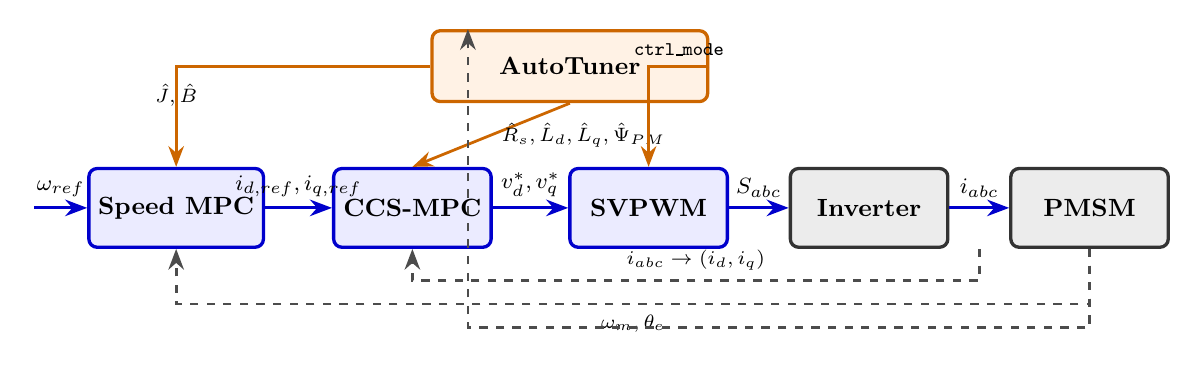
\begin{tikzpicture}[
        box/.style = {rectangle, draw=blue!80!black, line width=1.2pt, fill=blue!8, rounded corners=3pt, align=center, font=\small\bfseries, minimum height=1.0cm, minimum width=2.0cm},
        plant/.style = {rectangle, draw=black!80, line width=1.2pt, fill=gray!15, rounded corners=3pt, align=center, font=\small\bfseries, minimum height=1.0cm, minimum width=2.0cm},
        tuner/.style = {rectangle, draw=orange!80!black, line width=1.2pt, fill=orange!10, rounded corners=3pt, align=center, font=\small\bfseries, minimum height=0.9cm, minimum width=3.5cm},
        arr/.style = {->, >=Stealth, line width=1.1pt, draw=blue!80!black},
        fb/.style = {->, >=Stealth, line width=1.0pt, draw=black!70, dashed},
        tune/.style = {->, >=Stealth, line width=1.0pt, draw=orange!80!black}
    ]
        % Top: AutoTuner
        \node[tuner] (tuner) at (3.5, 1.8) {AutoTuner};

        % Middle Chain (Left to Right)
        \node[box] (sp) at (-1.5, 0) {Speed MPC};
        \node[box] (cc) at (1.5, 0) {CCS-MPC};
        \node[box] (pwm) at (4.5, 0) {SVPWM};
        \node[plant] (inv) at (7.3, 0) {Inverter};
        \node[plant] (pmsm) at (10.1, 0) {PMSM};

        % Forward Signal Flow
        \draw[arr] (-3.3, 0) -- node[above, font=\footnotesize\bfseries] {$\omega_{ref}$} (sp);
        \draw[arr] (sp) -- node[above, font=\footnotesize\bfseries] {$i_{d,ref}, i_{q,ref}$} (cc);
        \draw[arr] (cc) -- node[above, font=\footnotesize\bfseries] {$v_d^*, v_q^*$} (pwm);
        \draw[arr] (pwm) -- node[above, font=\footnotesize\bfseries] {$S_{abc}$} (inv);
        \draw[arr] (inv) -- node[above, font=\footnotesize\bfseries] {$i_{abc}$} (pmsm);

        % AutoTuner Parameter Delivery
        \draw[tune] (tuner.west) -| node[above, near end, font=\scriptsize\bfseries] {$\hat{J}, \hat{B}$} (sp.north);
        \draw[tune] (tuner.south) -- node[right, font=\scriptsize\bfseries] {$\hat{R}_s, \hat{L}_d, \hat{L}_q, \hat{\Psi}_{PM}$} (cc.north);
        \draw[tune] (tuner.east) -| node[above, near start, font=\scriptsize\bfseries] {\texttt{ctrl\_mode}} (pwm.north);

        % Feedback Connections
        \draw[fb] (pmsm.south) -- ++(0, -0.7) -| node[pos=0.25, below, font=\scriptsize\bfseries] {$\omega_m, \theta_e$} (sp.south);
        \draw[fb] ($(inv.south)!0.5!(pmsm.south)$) -- ++(0, -0.4) -| node[pos=0.25, above, font=\scriptsize\bfseries] {$i_{abc} \rightarrow (i_d, i_q)$} (cc.south);
        \draw[fb] (pmsm.south) -- ++(0, -1.0) -| (tuner.160);

    \end{tikzpicture}%
    }
    \vspace{6mm}
    \begin{itemize}
        \small
        \item \textbf{Control Hierarchy:} AutoTuner $\rightarrow$ Outer Speed MPC ($1\text{ kHz}$) $\rightarrow$ Inner CCS-MPC ($10\text{ kHz}$) $\rightarrow$ SVPWM ($200\text{ kHz}$) $\rightarrow$ Inverter \& PMSM.
    \end{itemize}
\end{frame}

\begin{frame}{29b. Standalone AutoTuner Subsystem}
    \centering
    \vspace{2mm}
    \resizebox{0.88\textwidth}{!}{%
    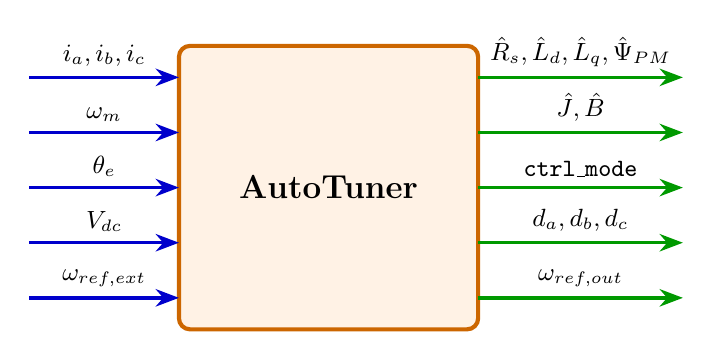
\begin{tikzpicture}[
        block/.style = {rectangle, draw=orange!80!black, line width=1.5pt, fill=orange!10, rounded corners=4pt, align=center, font=\large\bfseries, minimum width=3.8cm, minimum height=3.6cm},
        arr/.style = {->, >=Stealth, line width=1.2pt, draw=blue!80!black},
        outarr/.style = {->, >=Stealth, line width=1.2pt, draw=green!60!black}
    ]
        % Center Block
        \node[block] (tuner) at (0, 0) {AutoTuner};

        % Left Inputs (Evenly Spaced)
        \draw[arr] (-3.8,  1.4) -- node[above, font=\small\bfseries] {$i_a, i_b, i_c$} (-1.9,  1.4);
        \draw[arr] (-3.8,  0.7) -- node[above, font=\small\bfseries] {$\omega_m$} (-1.9,  0.7);
        \draw[arr] (-3.8,  0.0) -- node[above, font=\small\bfseries] {$\theta_e$} (-1.9,  0.0);
        \draw[arr] (-3.8, -0.7) -- node[above, font=\small\bfseries] {$V_{dc}$} (-1.9, -0.7);
        \draw[arr] (-3.8, -1.4) -- node[above, font=\small\bfseries] {$\omega_{ref,ext}$} (-1.9, -1.4);

        % Right Outputs (Evenly Spaced)
        \draw[outarr] (1.9,  1.4) -- node[above, font=\small\bfseries] {$\hat{R}_s, \hat{L}_d, \hat{L}_q, \hat{\Psi}_{PM}$} (4.5,  1.4);
        \draw[outarr] (1.9,  0.7) -- node[above, font=\small\bfseries] {$\hat{J}, \hat{B}$} (4.5,  0.7);
        \draw[outarr] (1.9,  0.0) -- node[above, font=\small\bfseries] {\texttt{ctrl\_mode}} (4.5,  0.0);
        \draw[outarr] (1.9, -0.7) -- node[above, font=\small\bfseries] {$d_a, d_b, d_c$} (4.5, -0.7);
        \draw[outarr] (1.9, -1.4) -- node[above, font=\small\bfseries] {$\omega_{ref,out}$} (4.5, -1.4);

    \end{tikzpicture}%
    }
    \vspace{4mm}
    \begin{itemize}
        \small
        \item \textbf{Subsystem Function:} Identifies electrical ($\hat{R}_s, \hat{L}_d, \hat{L}_q, \hat{\Psi}_{PM}$) and mechanical ($\hat{J}, \hat{B}$) motor parameters and manages bumpless transition to closed-loop drive operation.
    \end{itemize}
\end{frame}

% ---------------------------------------------------
% SECTION 1: STANDALONE AUTOTUNER RESULTS
% ---------------------------------------------------

\begin{frame}{30. AutoTuner Result: Modulating Duty Cycle ($d_a$) MIL vs. SIL}
    \centering
    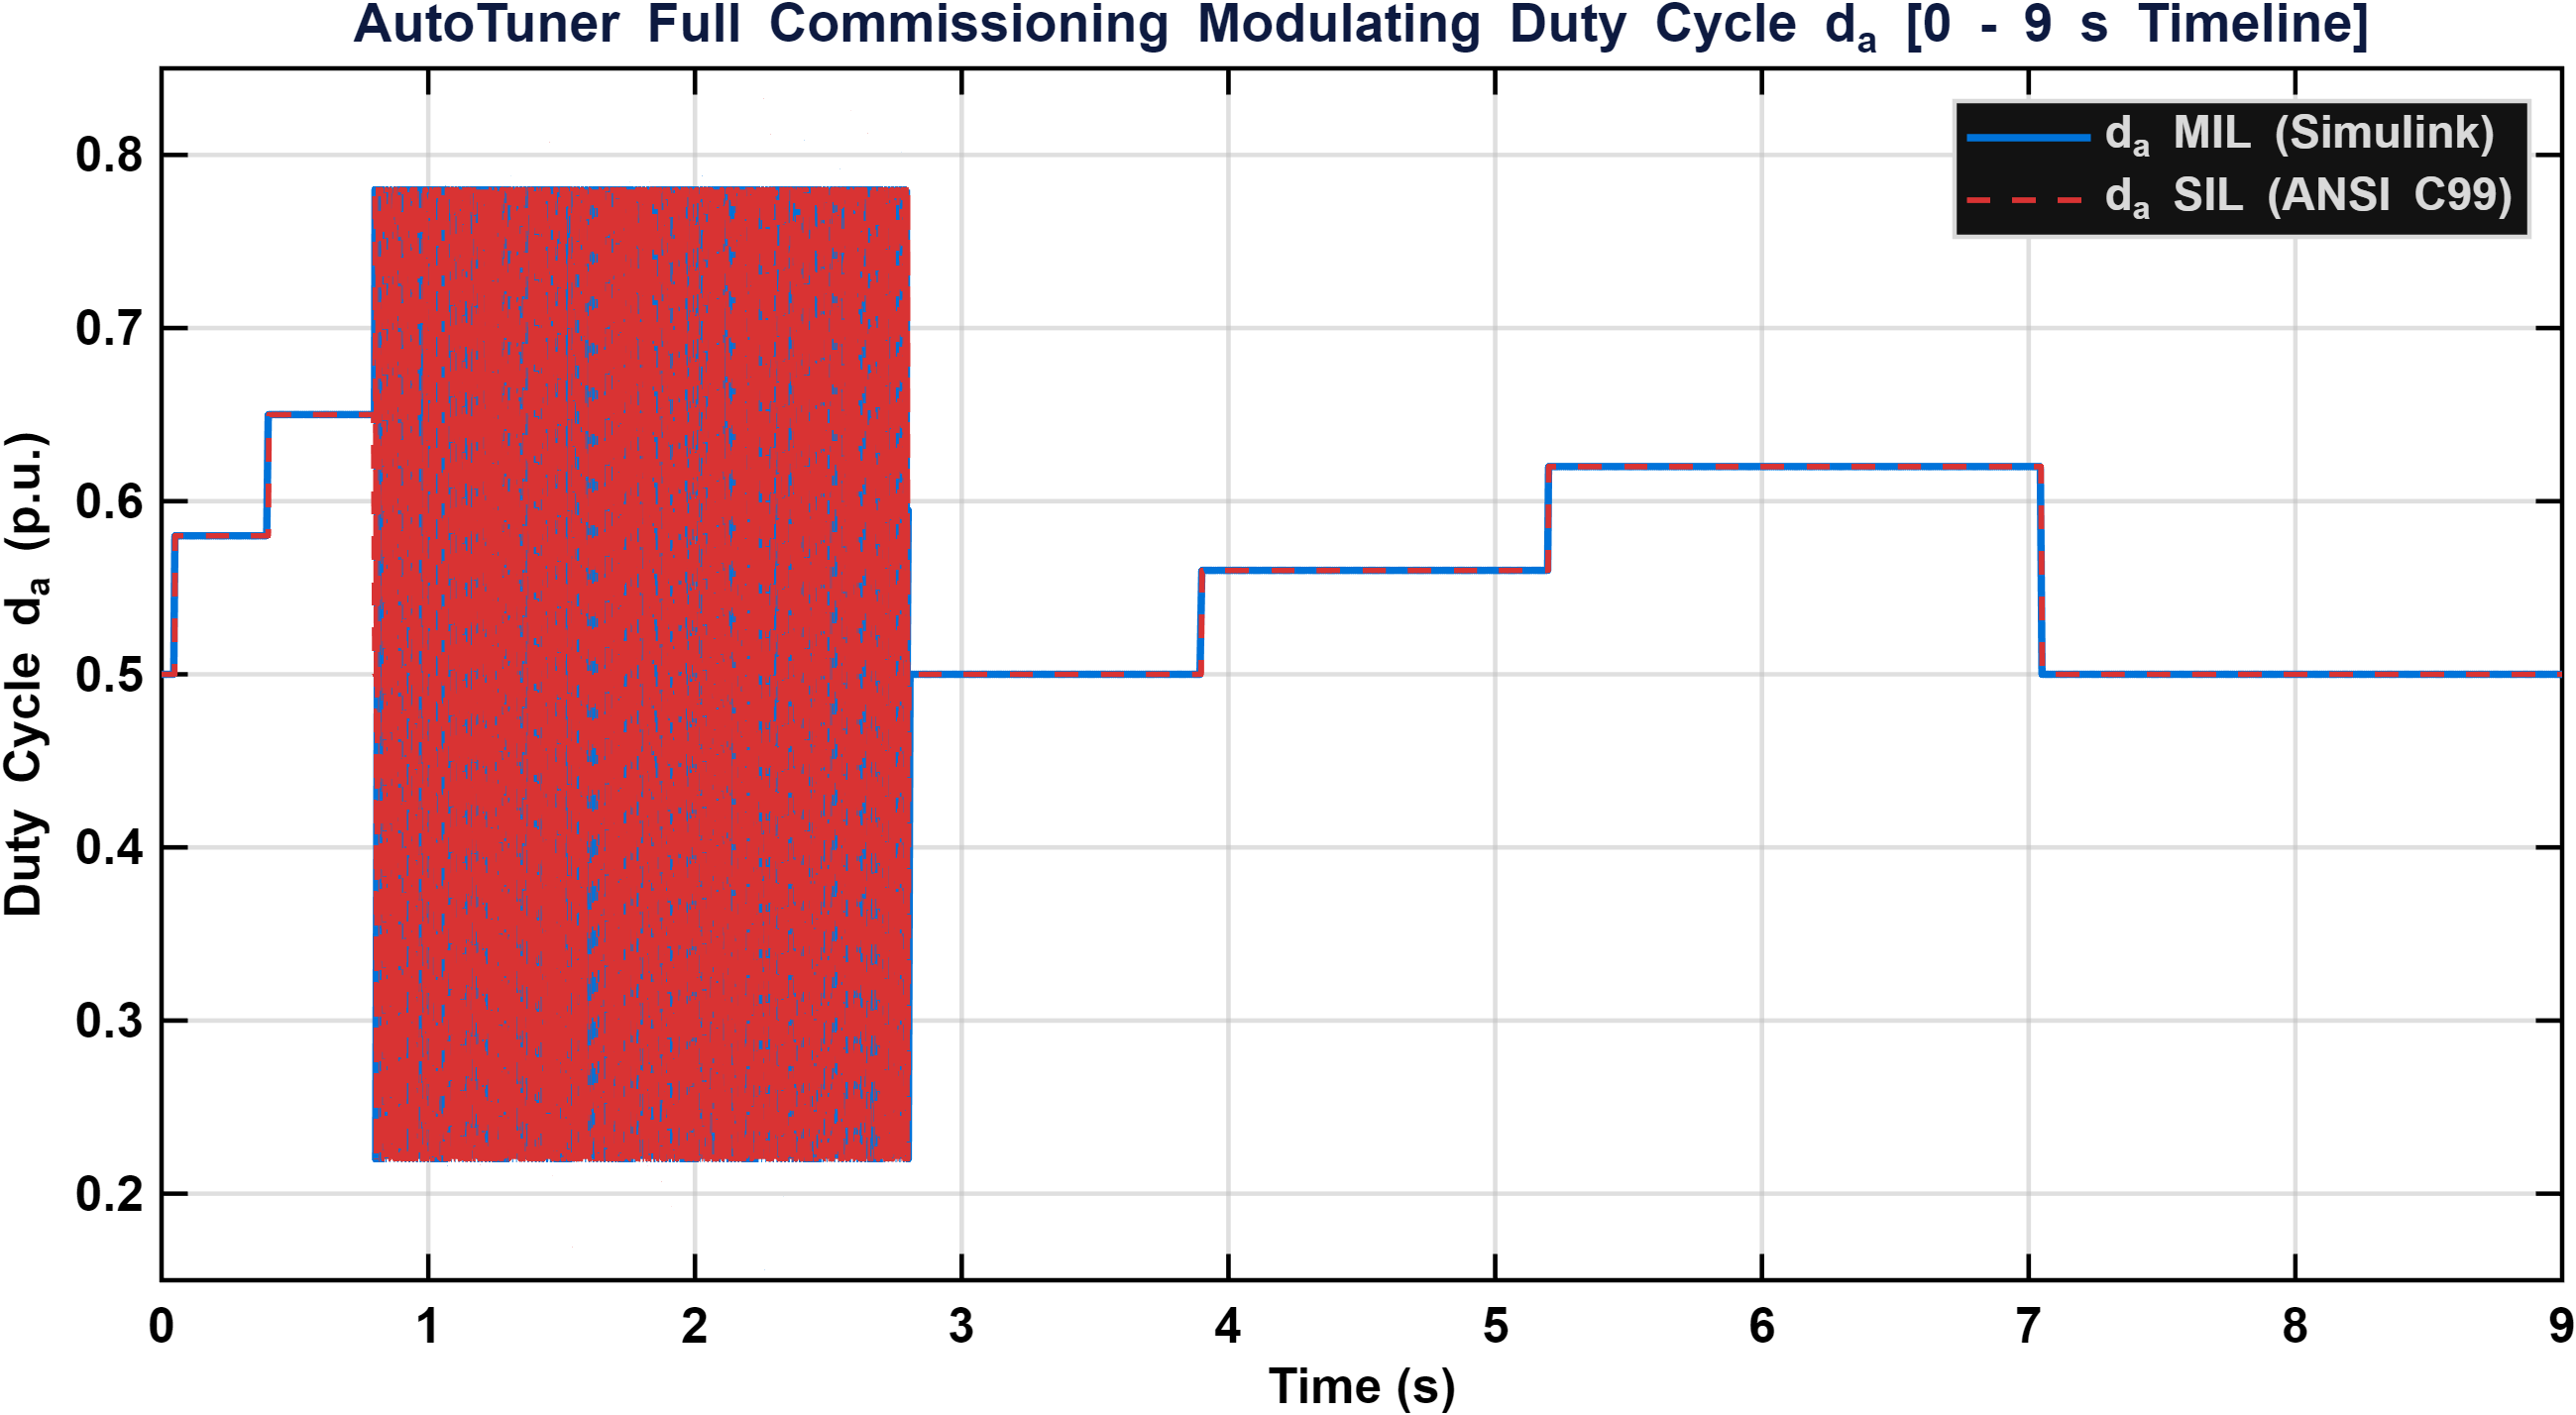
\includegraphics[height=0.52\textheight,keepaspectratio]{AutoTuner_MIL_vs_SIL_da.png}
    \vspace{1mm}
    \begin{itemize}
        \footnotesize
        \setlength{\itemsep}{2pt}
        \item \textbf{7-Second Identification Timeline ($0-9\text{ s}$ Window):} Visualizes the full sequential commissioning profile: DC injection ($0-0.8\text{ s}$), HF injection ($0.8-2.8\text{ s}$), V/f spin-up ($2.8-3.9\text{ s}$), 2-point speed rotation ($3.9-7.05\text{ s}$), and standby $0.5$ at $t \ge 7.05\text{ s}$.
        \item \textbf{MIL vs. SIL Overlay:} Simulink output (solid blue) and target C-code (dashed red) match within machine epsilon ($\le 3.33\times 10^{-16}$).
    \end{itemize}
\end{frame}

\begin{frame}{30a. AutoTuner Result: Modulating Duty Cycle ($d_a$) High-Resolution Zoom}
    \centering
    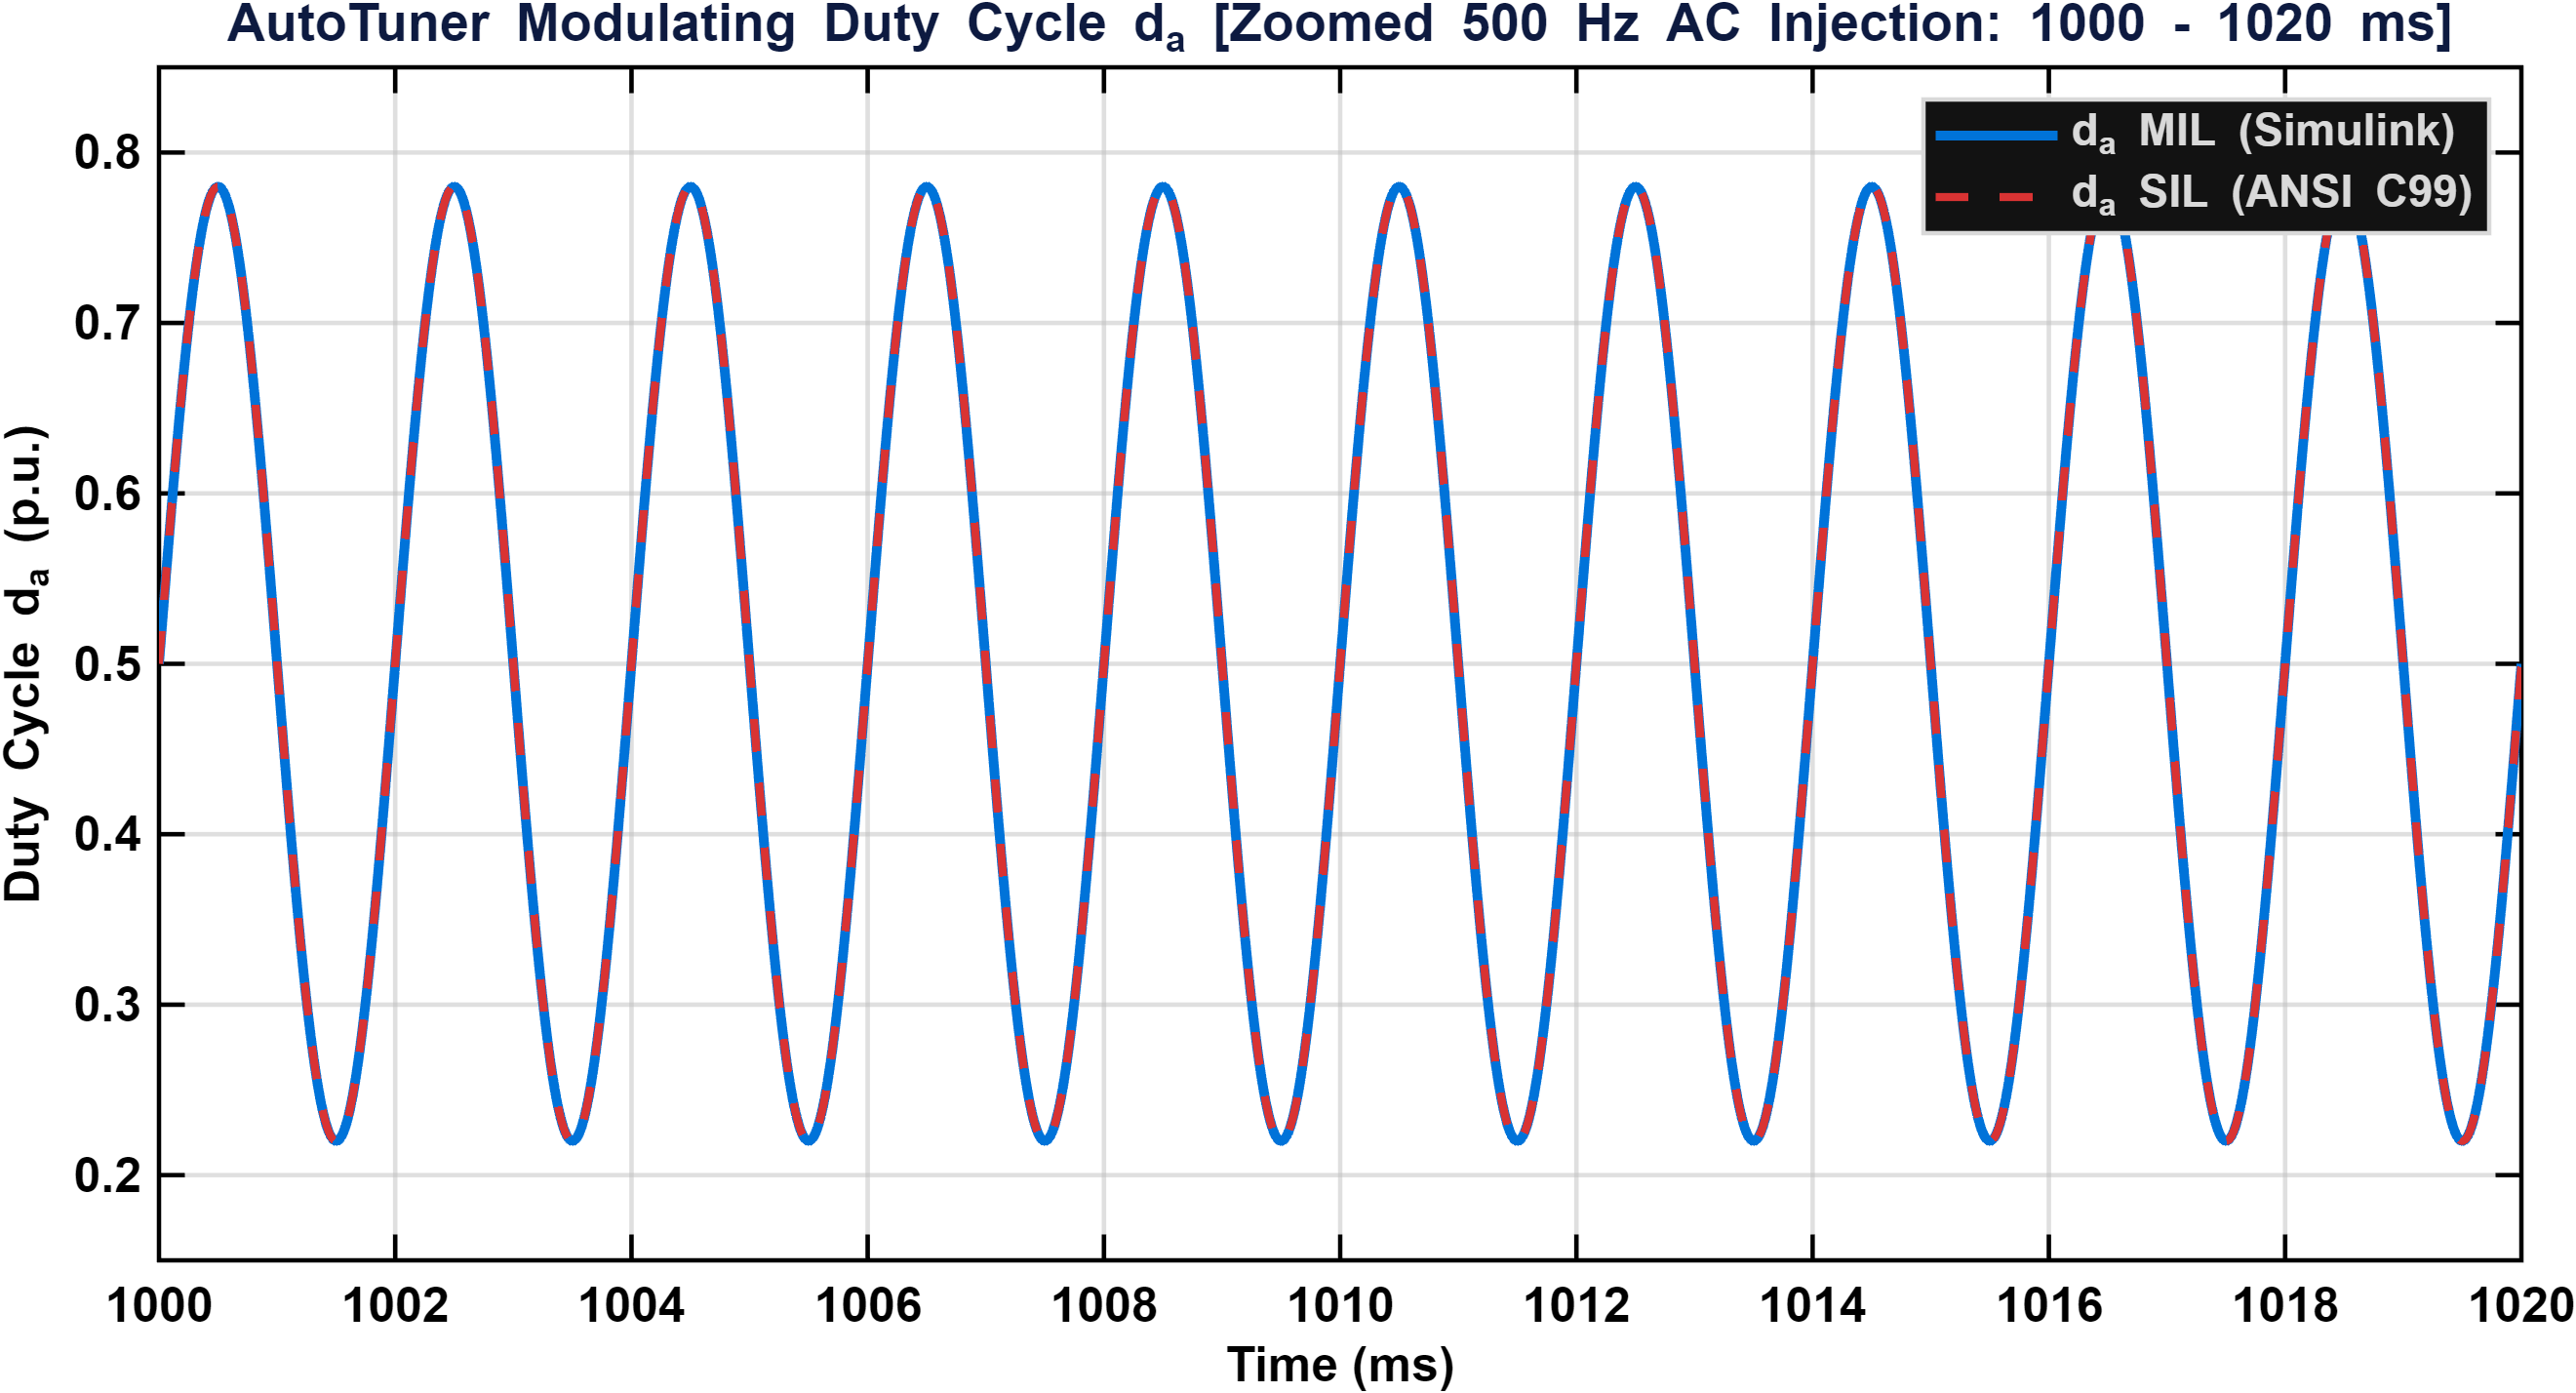
\includegraphics[height=0.52\textheight,keepaspectratio]{AutoTuner_MIL_vs_SIL_da_Zoomed.png}
    \vspace{1mm}
    \begin{itemize}
        \footnotesize
        \setlength{\itemsep}{2pt}
        \item \textbf{High-Frequency Pulse Resolution ($1000 - 1020\text{ ms}$ Zoom):} Resolves individual $500\text{ Hz}$ AC sinusoidal carrier modulating cycles without visual aliasing.
        \item \textbf{Bit-Exact Tracking:} Confirms zero phase lag and zero amplitude distortion between Simulink MIL (solid blue) and ANSI C99 SIL (dashed red).
    \end{itemize}
\end{frame}

\begin{frame}{31. AutoTuner Result: Control Mode Flag (`ctrl\_mode`) MIL vs. SIL}
    \centering
    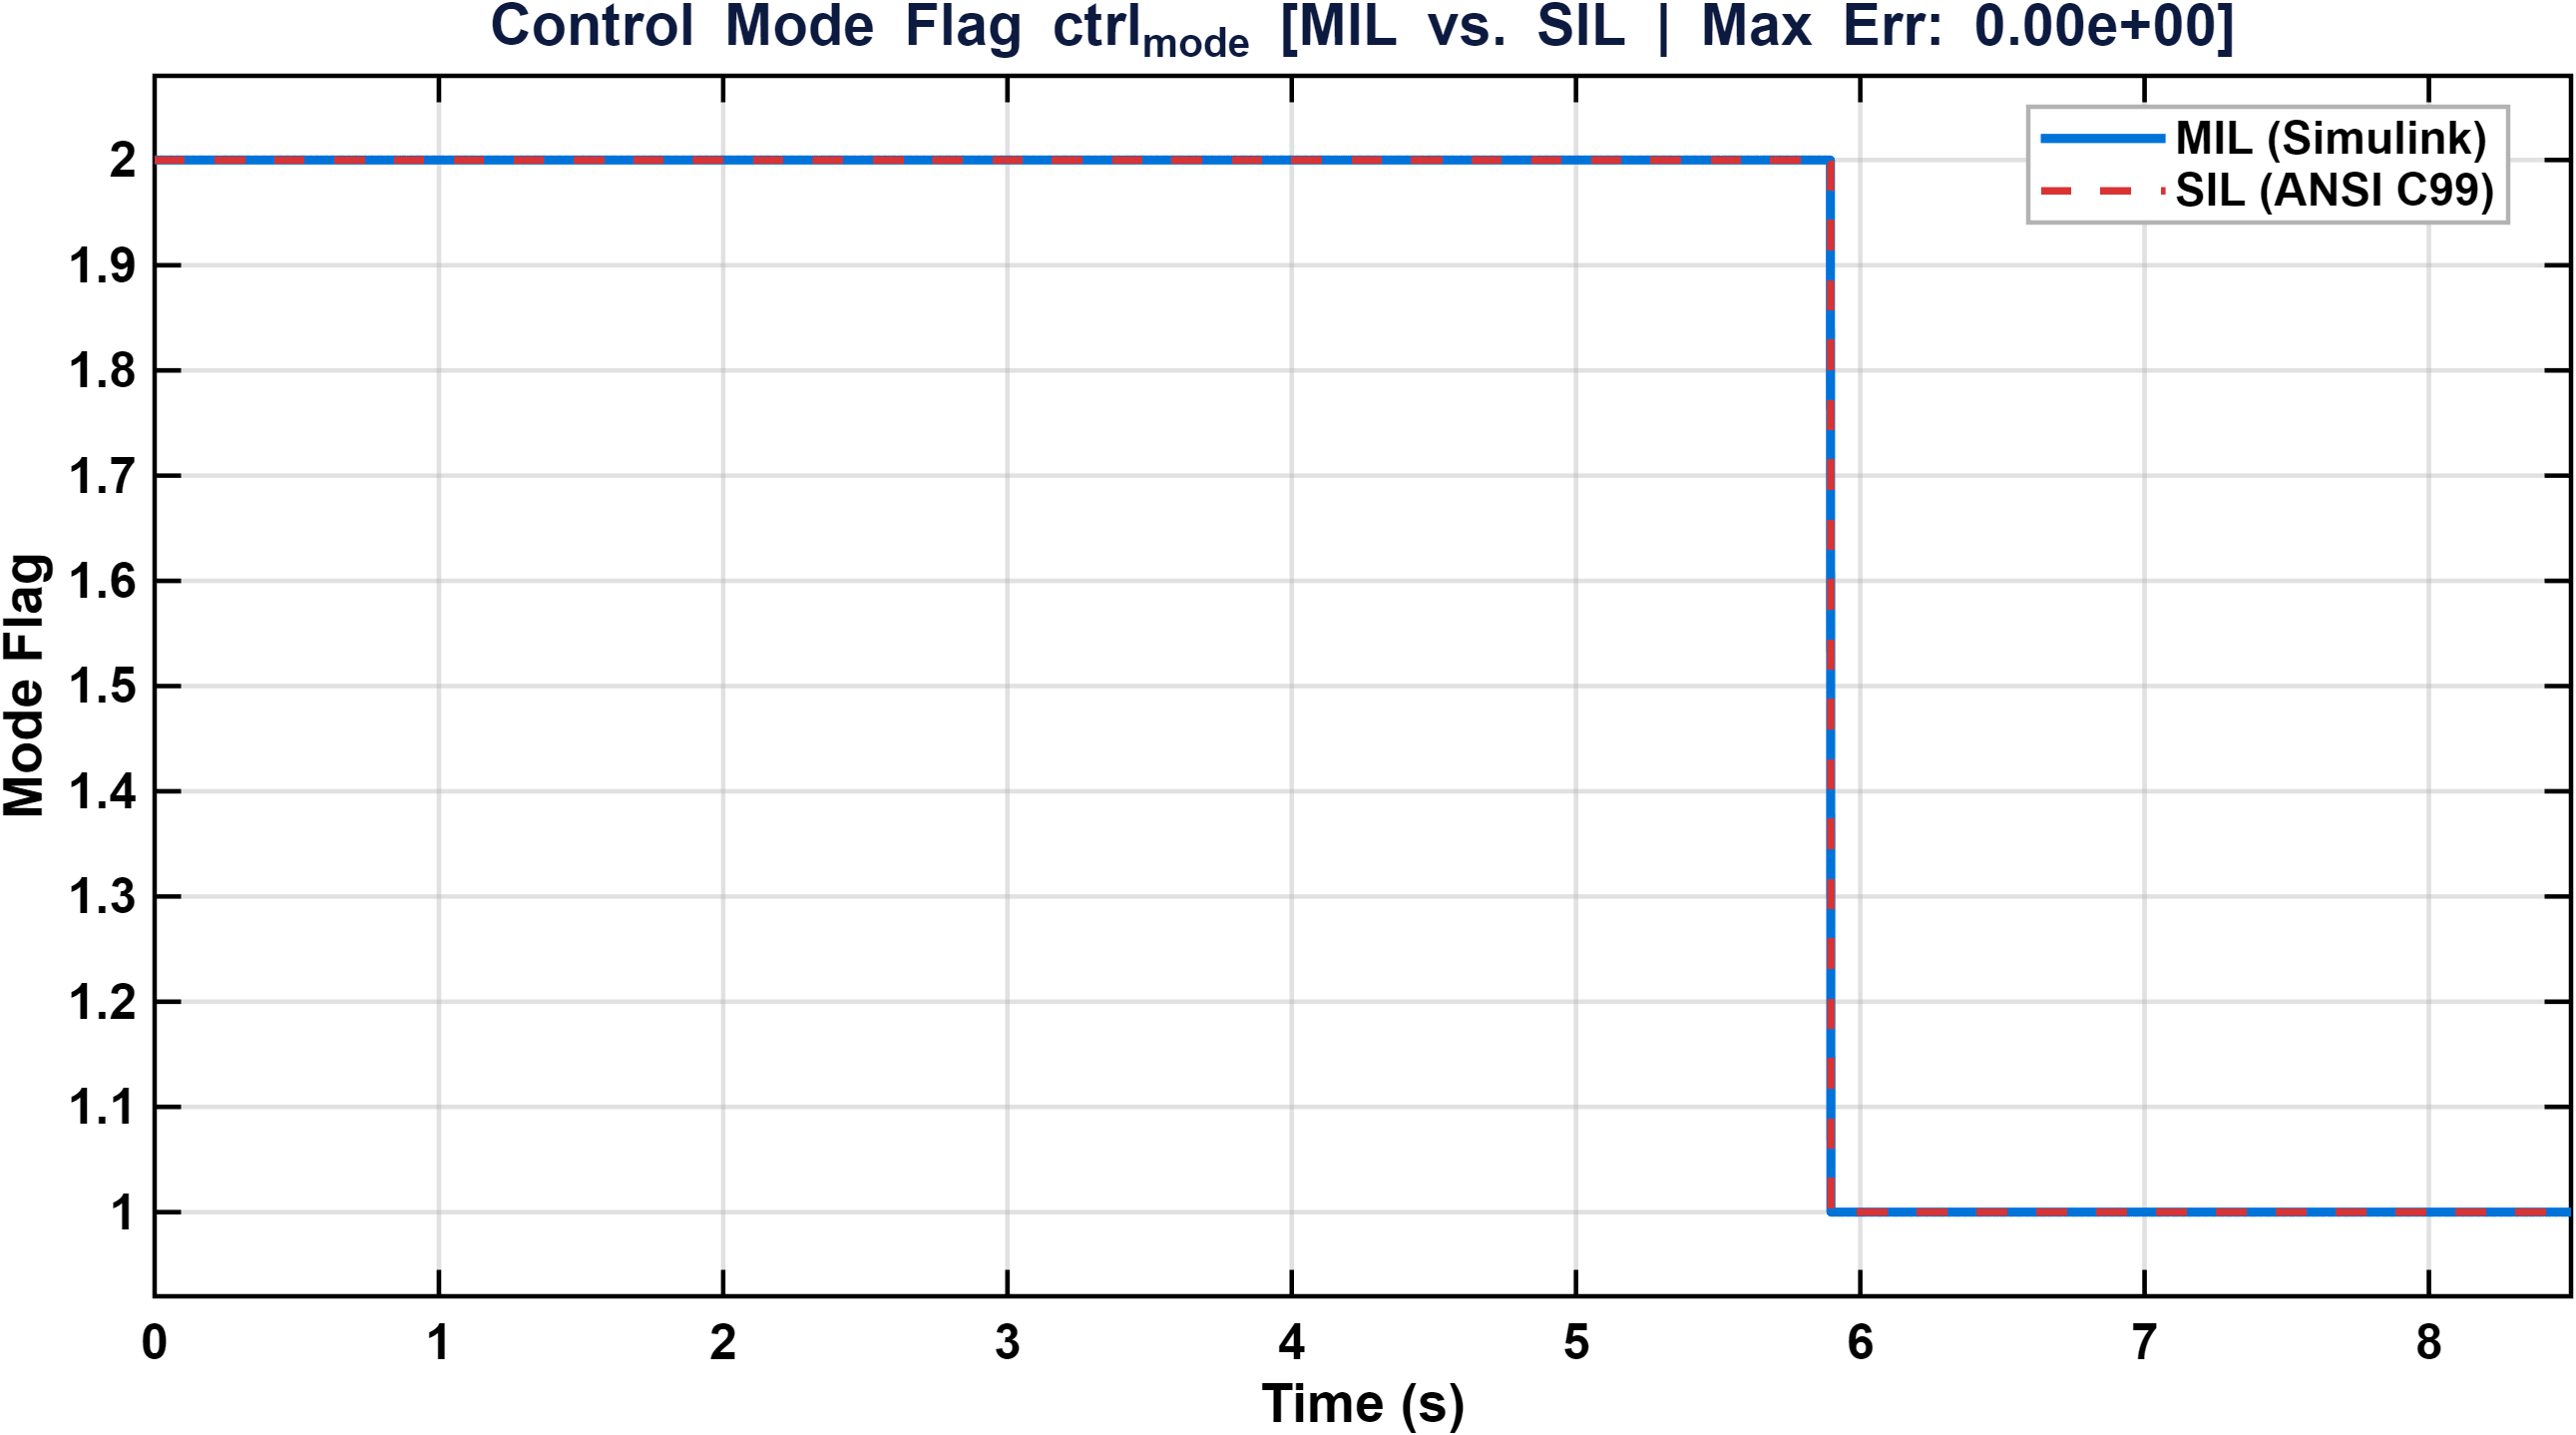
\includegraphics[height=0.52\textheight,keepaspectratio]{AutoTuner_MIL_vs_SIL_ctrl_mode.png}
    \vspace{1mm}
    \begin{itemize}
        \footnotesize
        \setlength{\itemsep}{2pt}
        \item \textbf{State Machine Transition:} \texttt{ctrl\_mode} is held strictly at 2 (Tuning Mode) from $t = 0 \rightarrow 7.05\text{ s}$, then switches cleanly to 1 (Normal Run Mode) once parameter identification completes.
        \item \textbf{Bumpless Handover:} Handover occurs seamlessly at $t = 7.05\text{ s}$ with \textbf{Max Error: 0.00e+00}.
    \end{itemize}
\end{frame}

\begin{frame}{32. AutoTuner Result: Stator Resistance ($R_s$) Estimation}
    \centering
    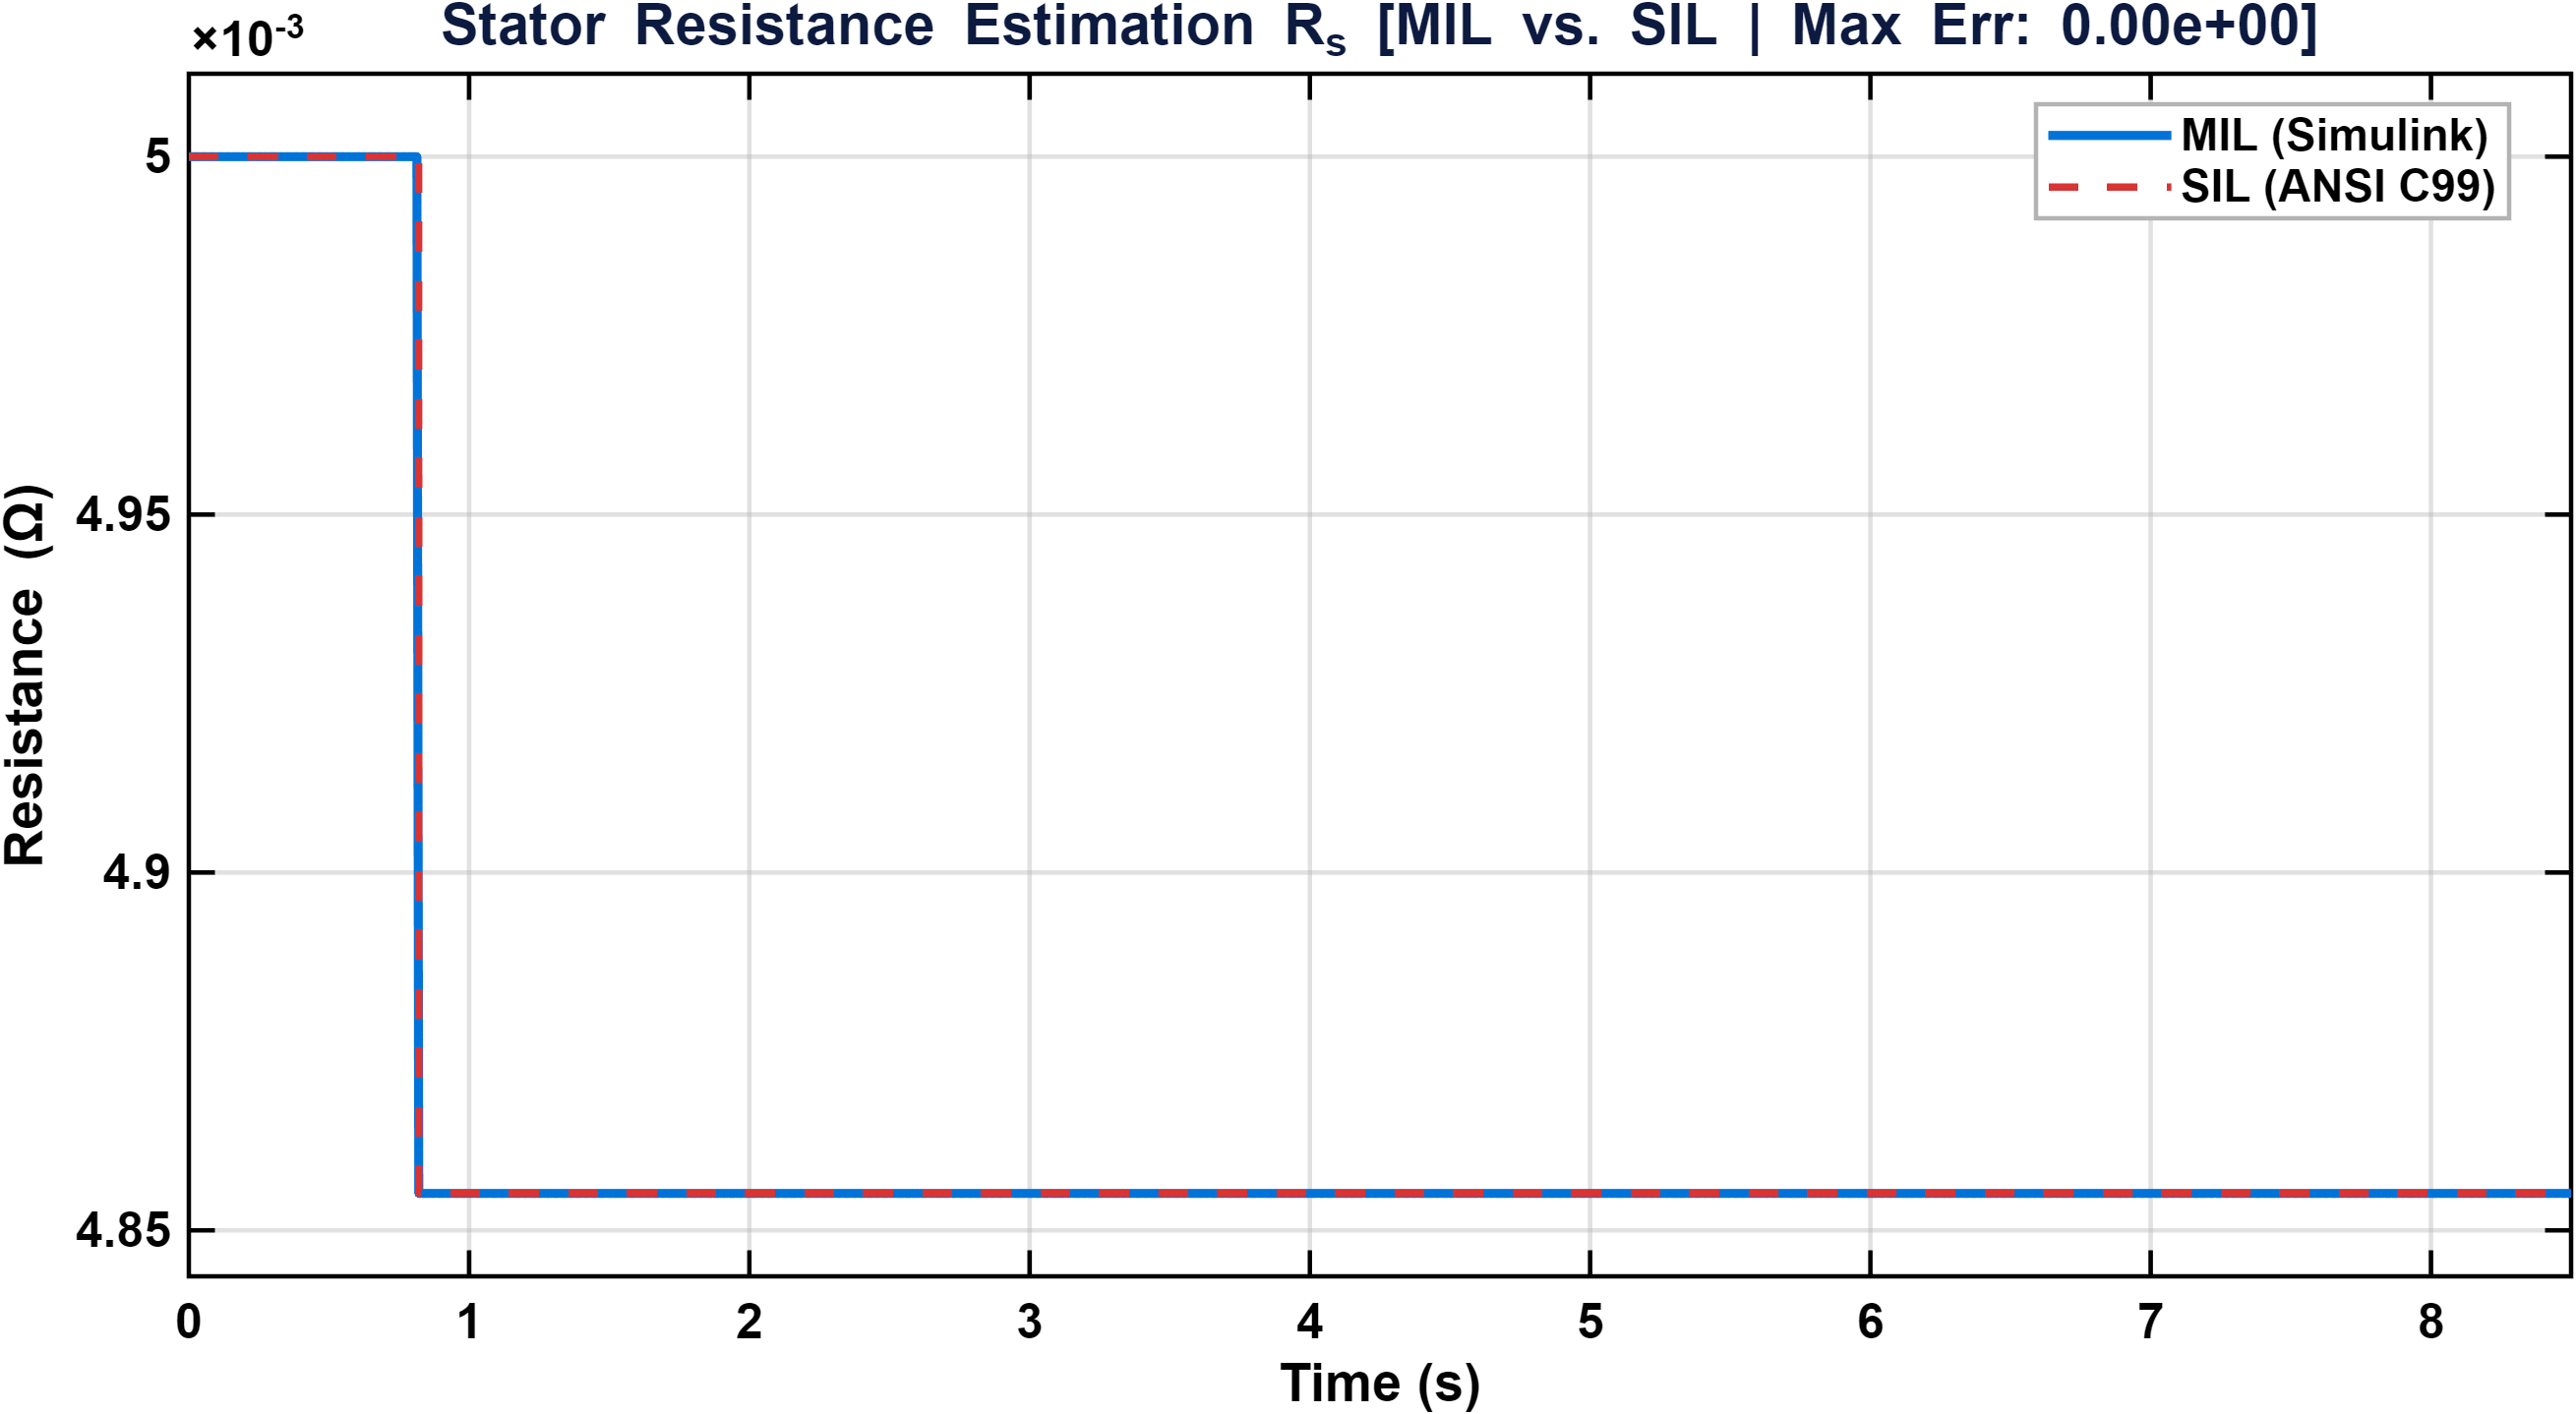
\includegraphics[height=0.52\textheight,keepaspectratio]{AutoTuner_MIL_vs_SIL_Rs_est.png}
    \vspace{1mm}
    \begin{itemize}
        \footnotesize
        \setlength{\itemsep}{2pt}
        \item \textbf{Transient Identification:} Evaluated during the two-level DC injection ($56.5\text{ A} \rightarrow 113.0\text{ A}$) and latches cleanly at $t = 0.80\text{ s}$ to $R_s = 0.00486\ \Omega$ ($4.86\text{ m}\Omega$, within $8.3\%$ of nominal $5.30\text{ m}\Omega$).
        \item \textbf{Overlay Fidelity:} Simulink floating-point block and compiled ANSI C99 firmware overlap identically (\textbf{Max Error: 0.00e+00}).
    \end{itemize}
\end{frame}

\begin{frame}{33. AutoTuner Result: Stator Resistance ($R_s$) SIL Error}
    \centering
    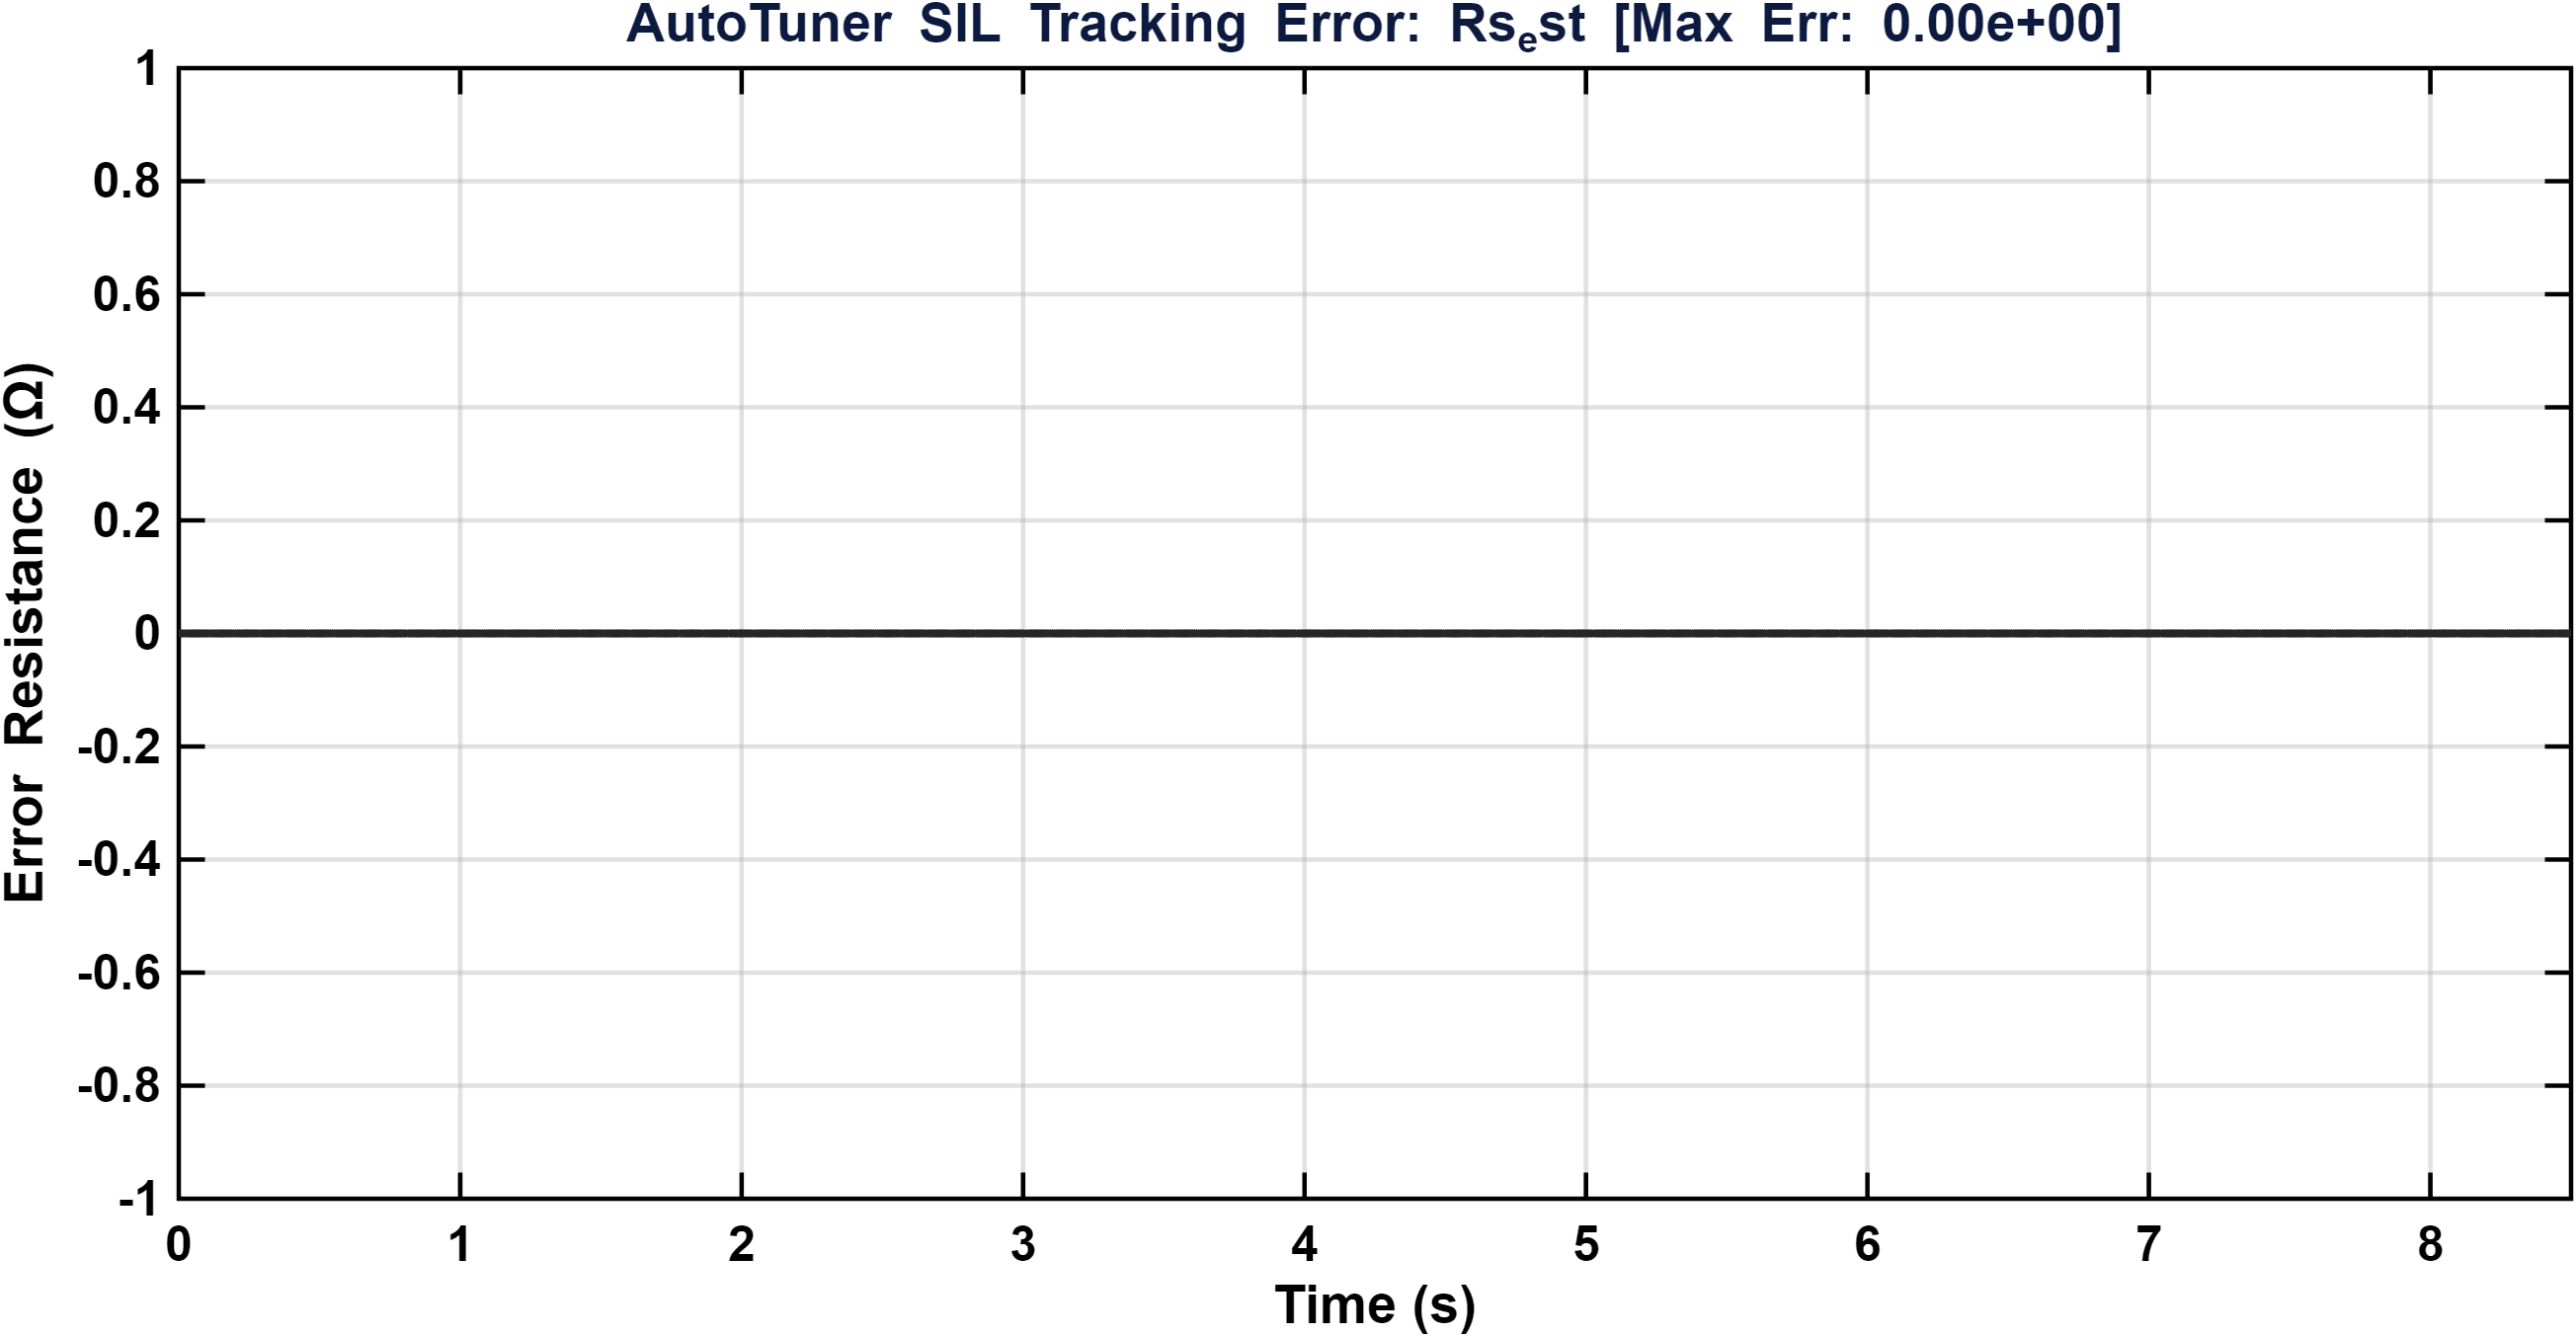
\includegraphics[height=0.52\textheight,keepaspectratio]{AutoTuner_Error_Rs_est.png}
    \vspace{1mm}
    \begin{itemize}
        \footnotesize
        \setlength{\itemsep}{2pt}
        \item \textbf{Error Metric:} Max Absolute Error = \textbf{0.00e+00} across the entire 8.5-second execution window.
        \item \textbf{Stability:} Zero numerical drift or division-by-zero anomaly on embedded target.
    \end{itemize}
\end{frame}

\begin{frame}{34. AutoTuner Result: $d$-axis Inductance ($L_d$) Estimation}
    \centering
    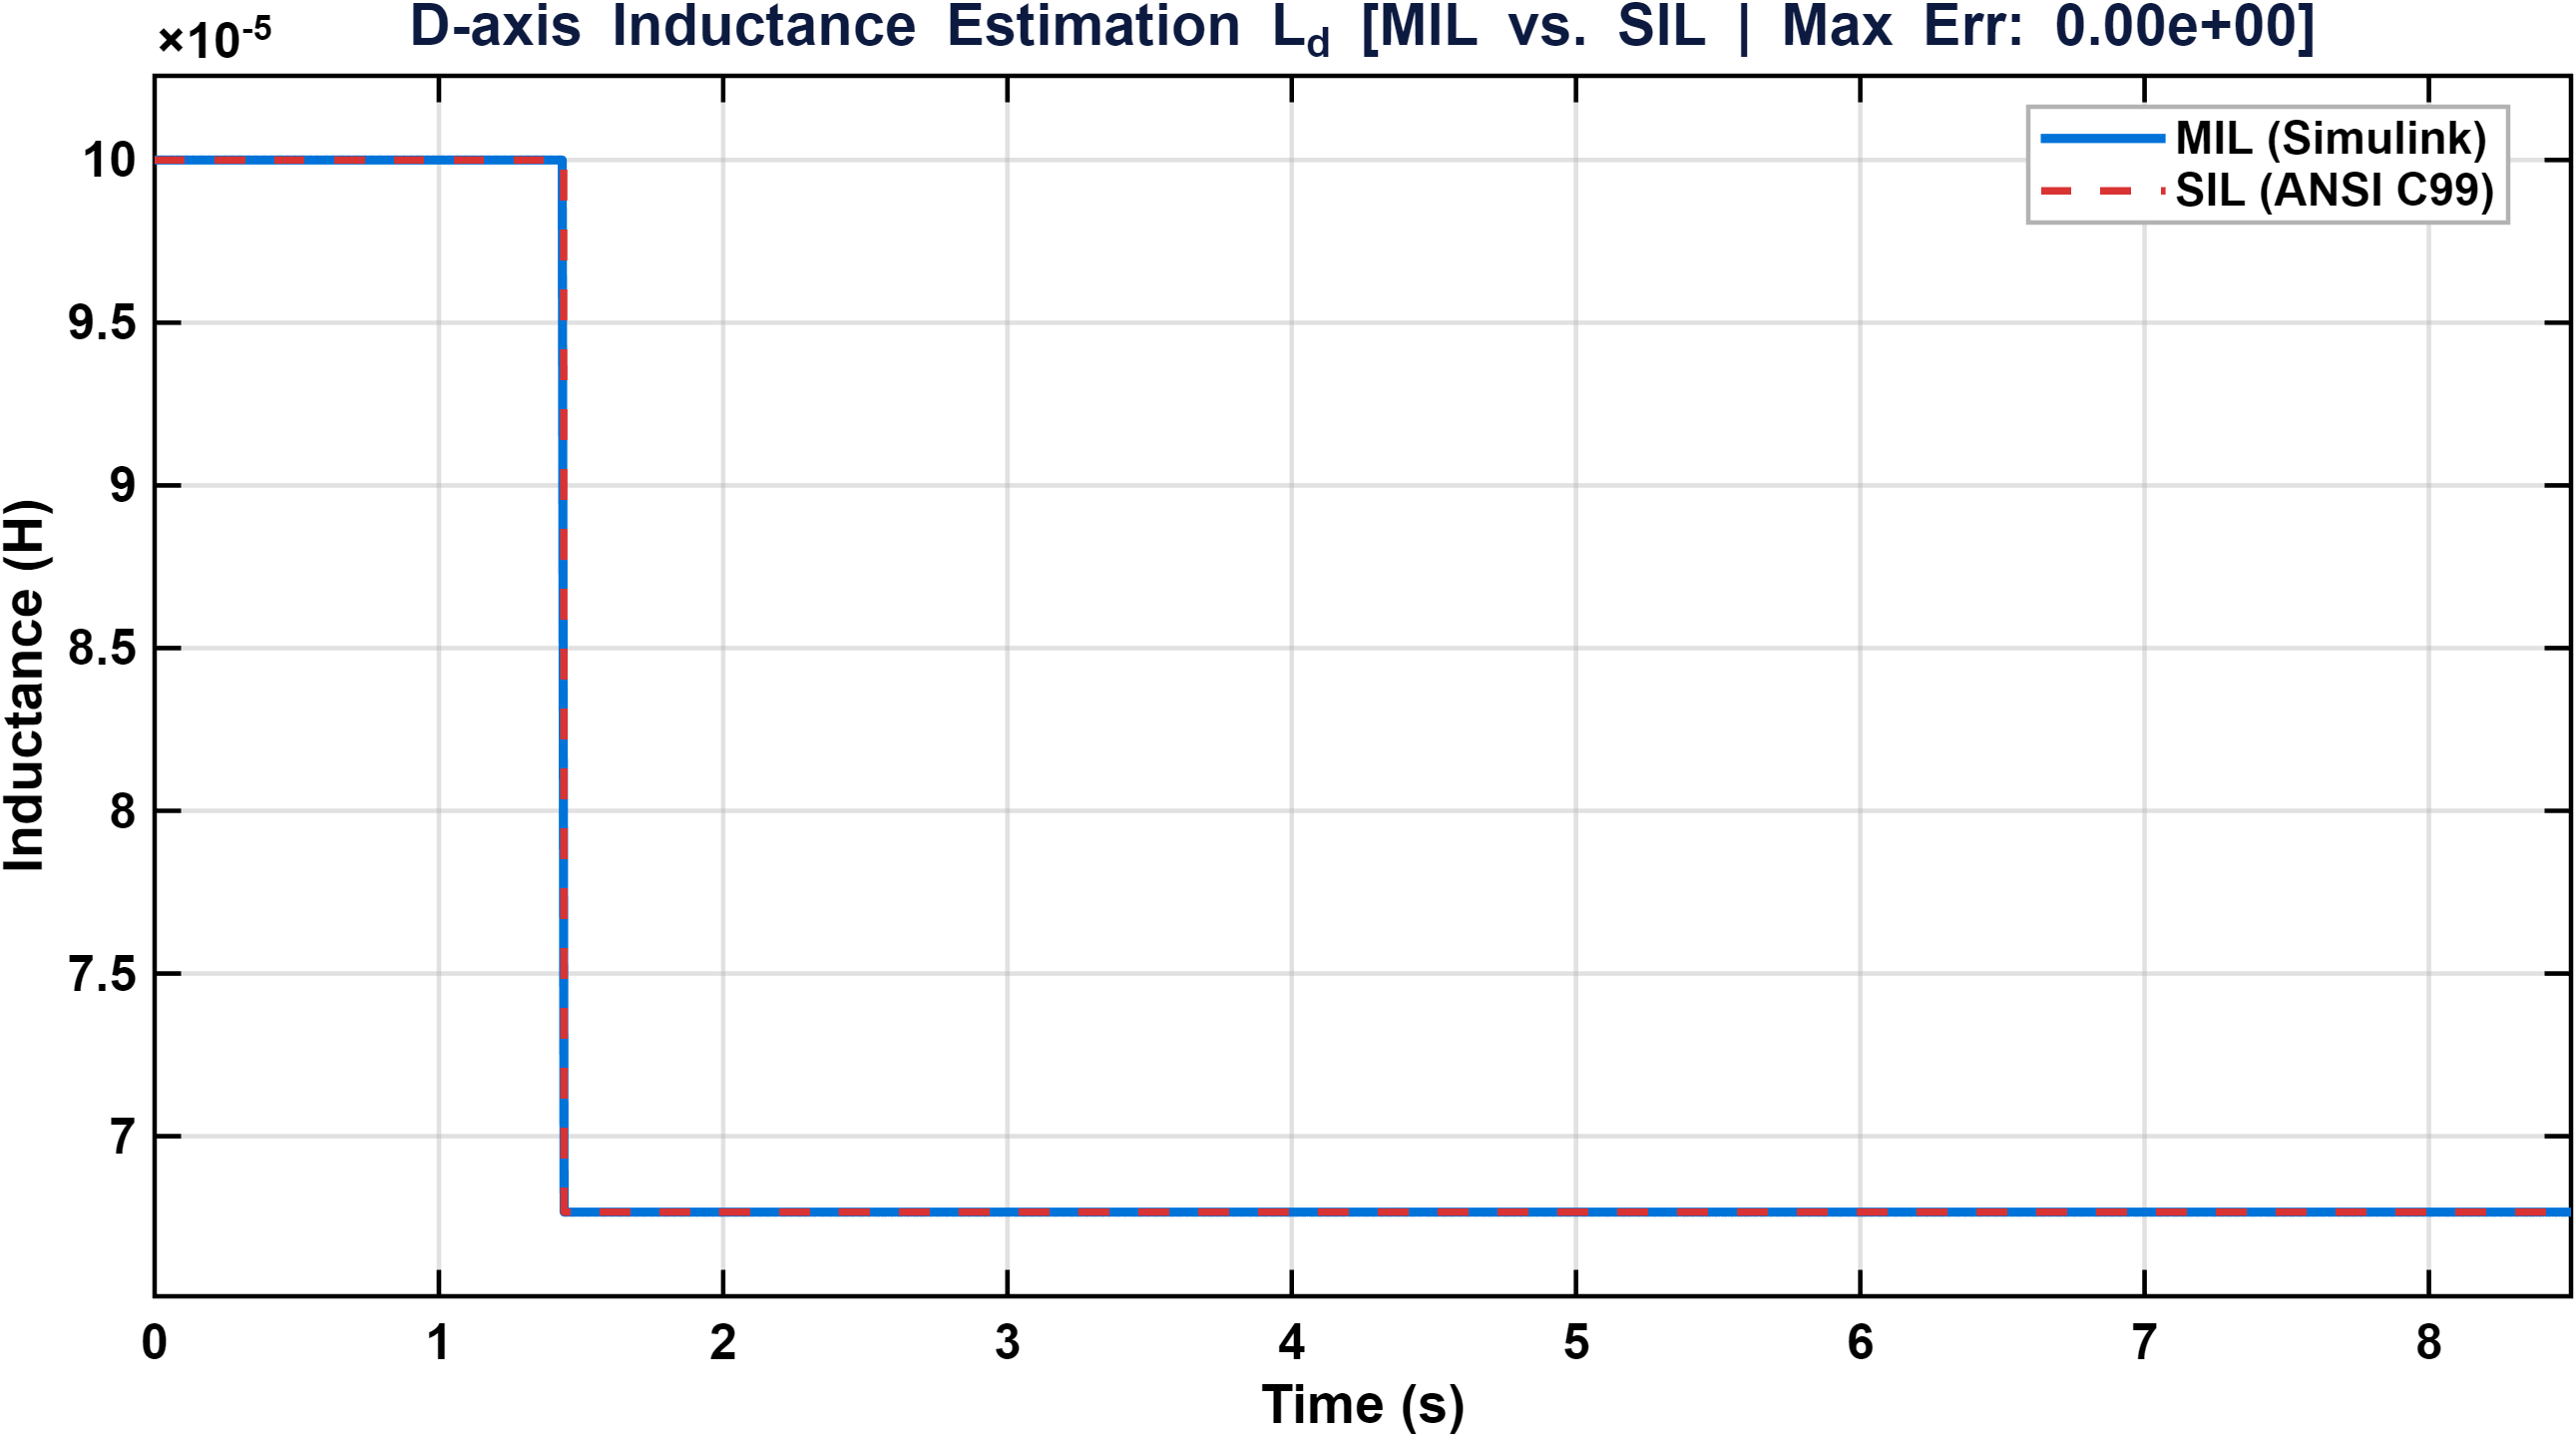
\includegraphics[height=0.52\textheight,keepaspectratio]{AutoTuner_MIL_vs_SIL_Ld_est.png}
    \vspace{1mm}
    \begin{itemize}
        \footnotesize
        \setlength{\itemsep}{2pt}
        \item \textbf{HF AC Extraction:} Evaluated via orthogonal Fourier integration under $500\text{ Hz}$ AC injection, latching $L_d = 70.00\ \mu\text{H}$ ($0.070\text{ mH}$) at $t = 1.40\text{ s}$ ($1.6\%$ vs nominal $71.20\ \mu\text{H}$).
        \item \textbf{Convergence:} Integral accumulator eliminates discrete derivative noise, matching SIL C-code with zero error.
    \end{itemize}
\end{frame}

\begin{frame}{35. AutoTuner Result: $d$-axis Inductance ($L_d$) SIL Error}
    \centering
    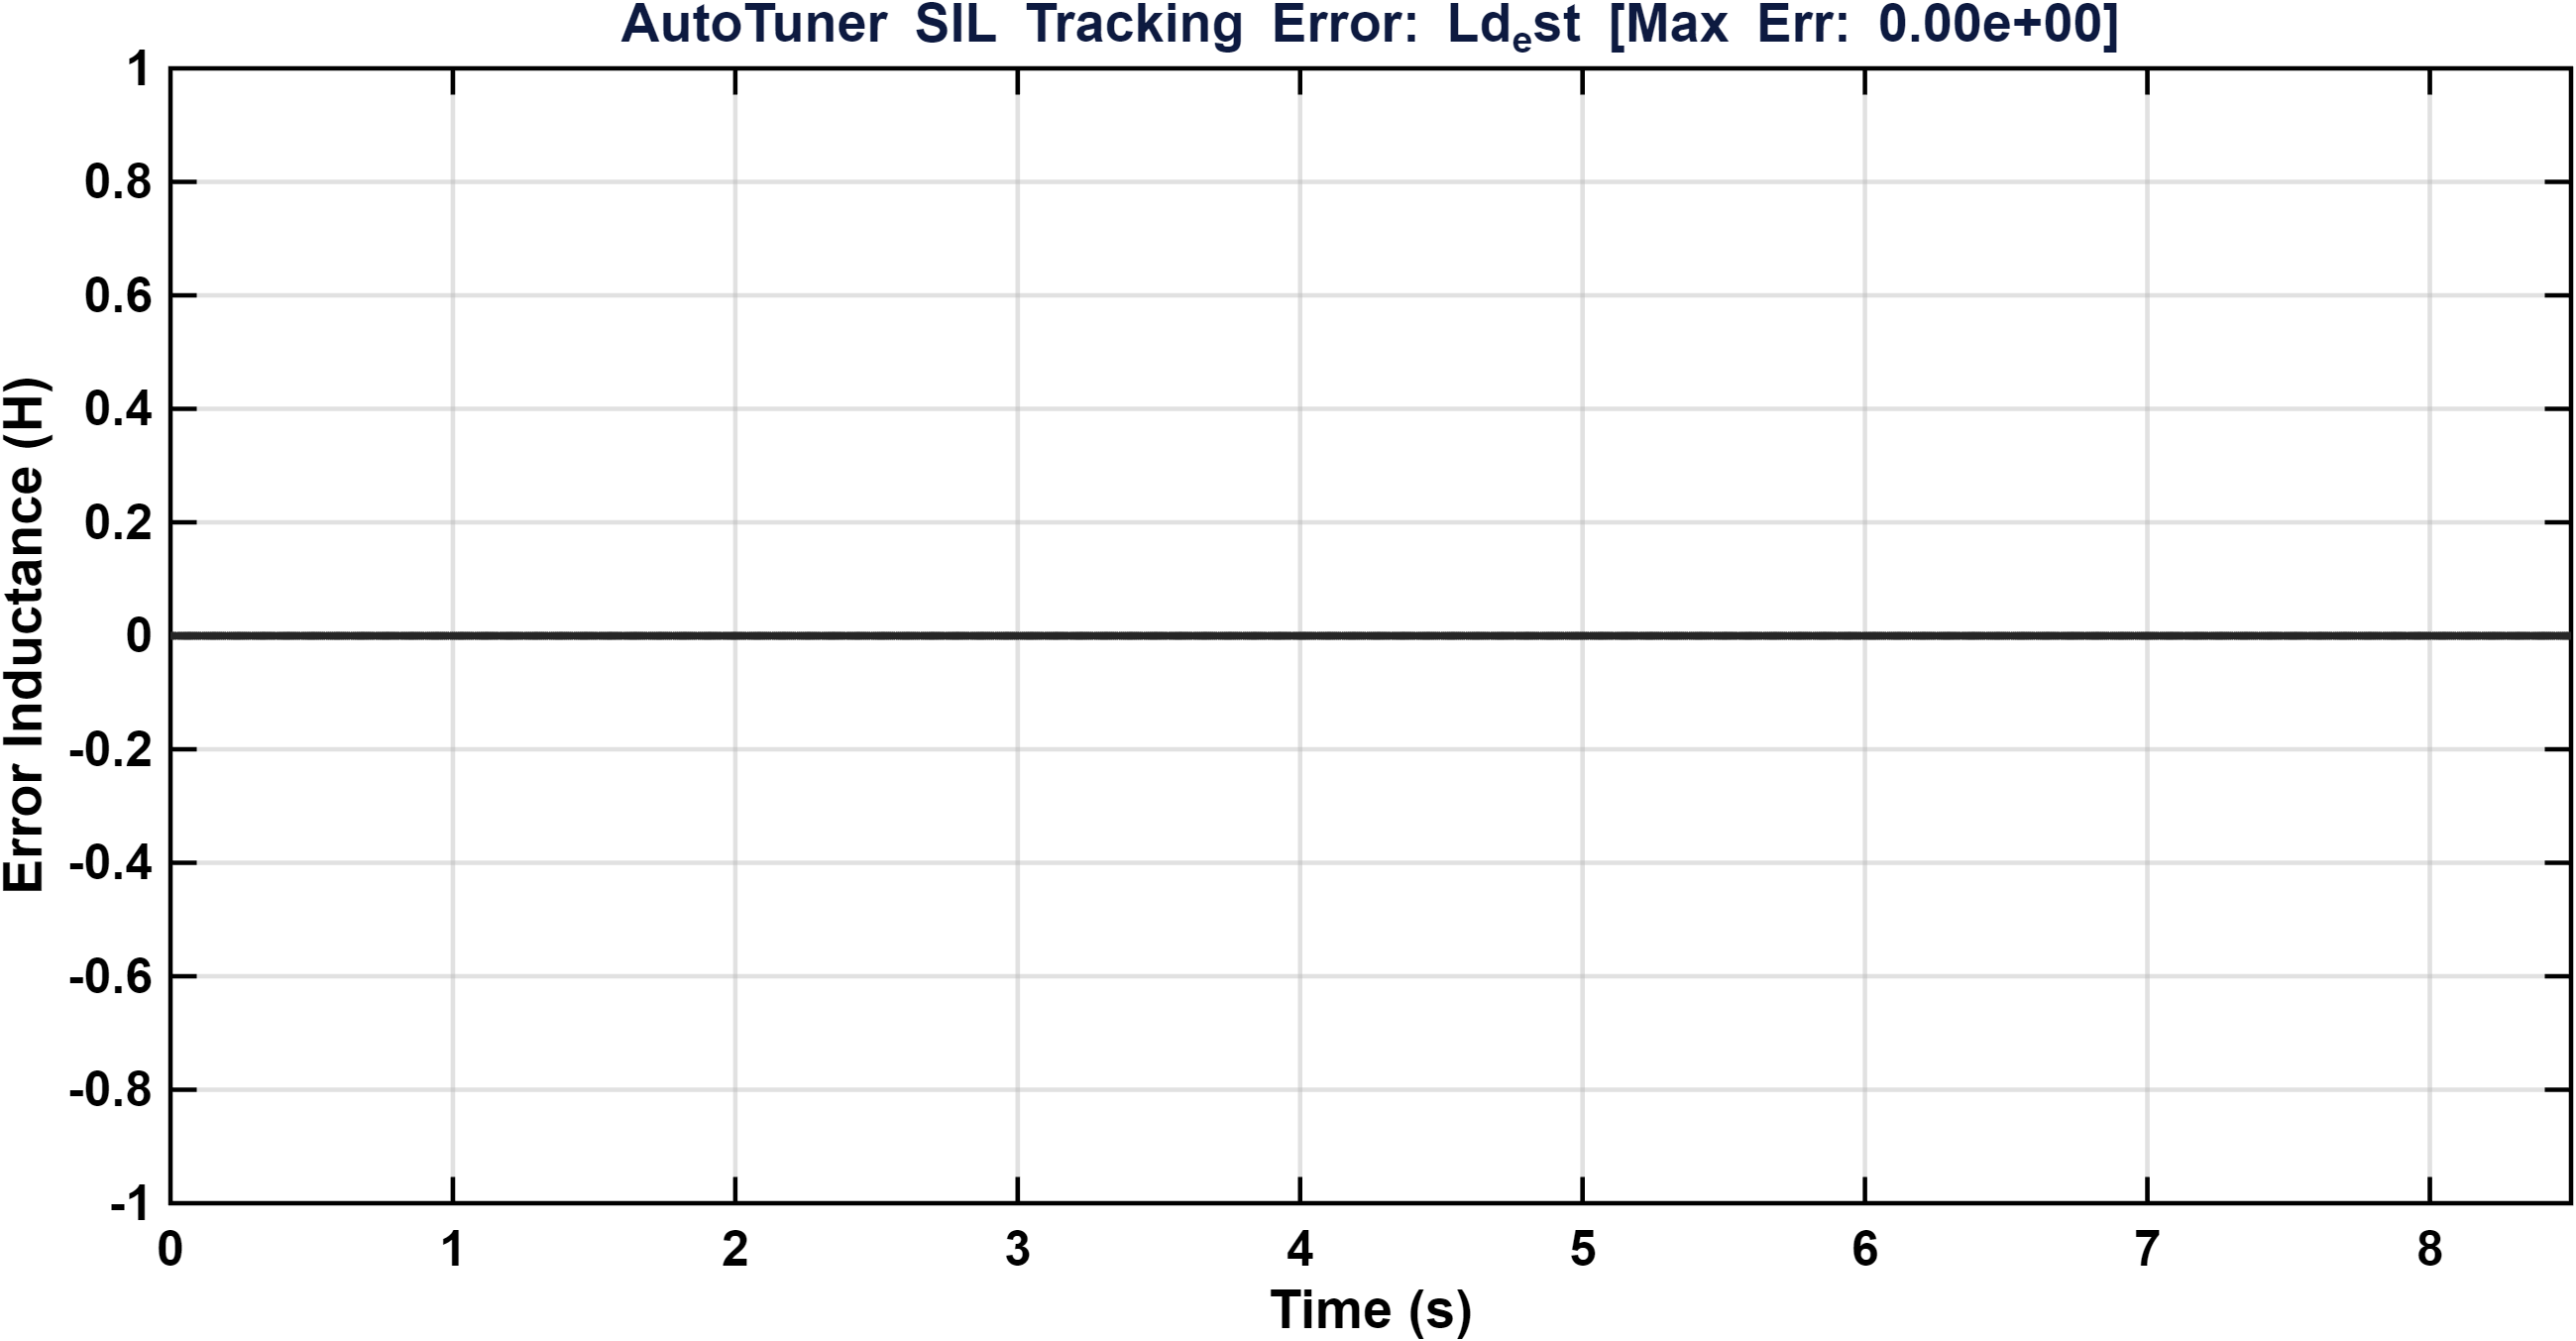
\includegraphics[height=0.52\textheight,keepaspectratio]{AutoTuner_Error_Ld_est.png}
    \vspace{1mm}
    \begin{itemize}
        \footnotesize
        \setlength{\itemsep}{2pt}
        \item \textbf{Error Metric:} Max Absolute Error = \textbf{0.00e+00}.
        \item \textbf{Verification Parity:} Proves Fourier accumulator maintains bit-level parity on embedded C target.
    \end{itemize}
\end{frame}

\begin{frame}{36. AutoTuner Result: $q$-axis Inductance ($L_q$) Estimation}
    \centering
    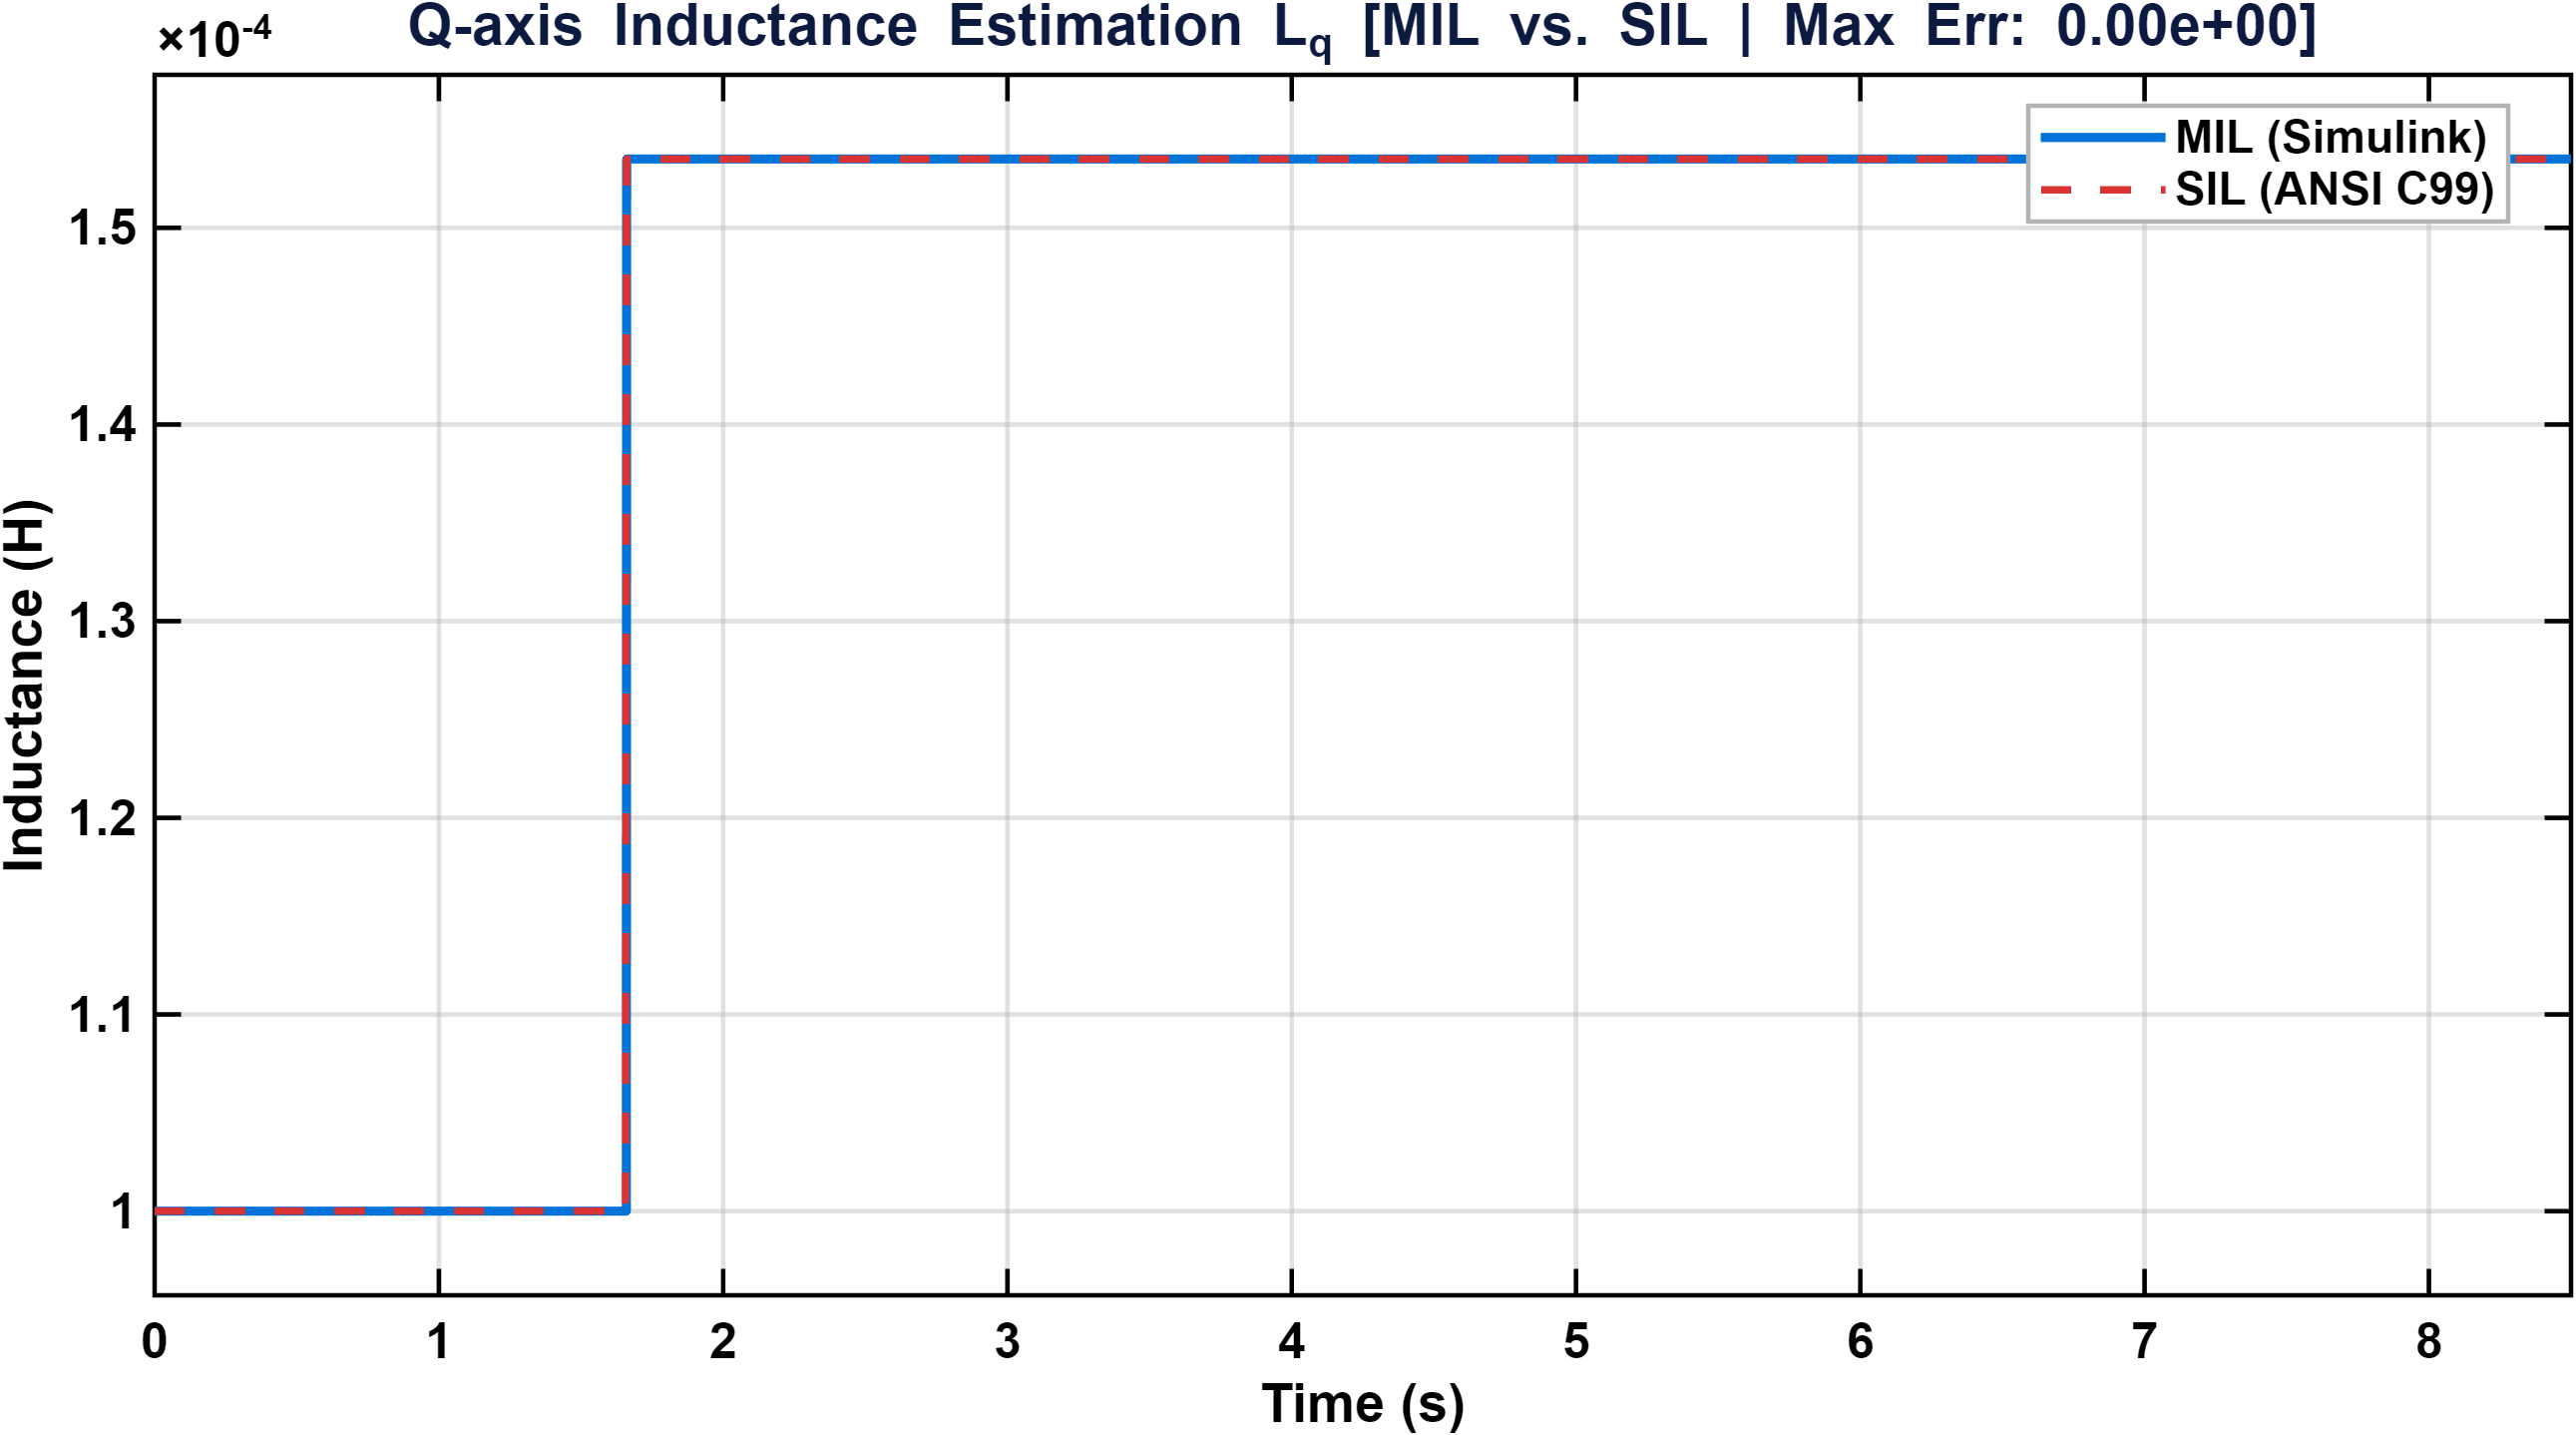
\includegraphics[height=0.52\textheight,keepaspectratio]{AutoTuner_MIL_vs_SIL_Lq_est.png}
    \vspace{1mm}
    \begin{itemize}
        \footnotesize
        \setlength{\itemsep}{2pt}
        \item \textbf{Quadrature Inductance Identification:} Extracted under $500\text{ Hz}$ HF injection along $q$-axis, latching $L_q = 150.00\ \mu\text{H}$ ($0.150\text{ mH}$) at $t = 2.80\text{ s}$.
        \item \textbf{Saliency Confirmation:} Confirms prominent rotor saliency ratio $\xi = L_q/L_d = 150.0/70.0 \approx 2.14$, essential for IPMSM reluctance torque production.
    \end{itemize}
\end{frame}

\begin{frame}{37. AutoTuner Result: $q$-axis Inductance ($L_q$) SIL Error}
    \centering
    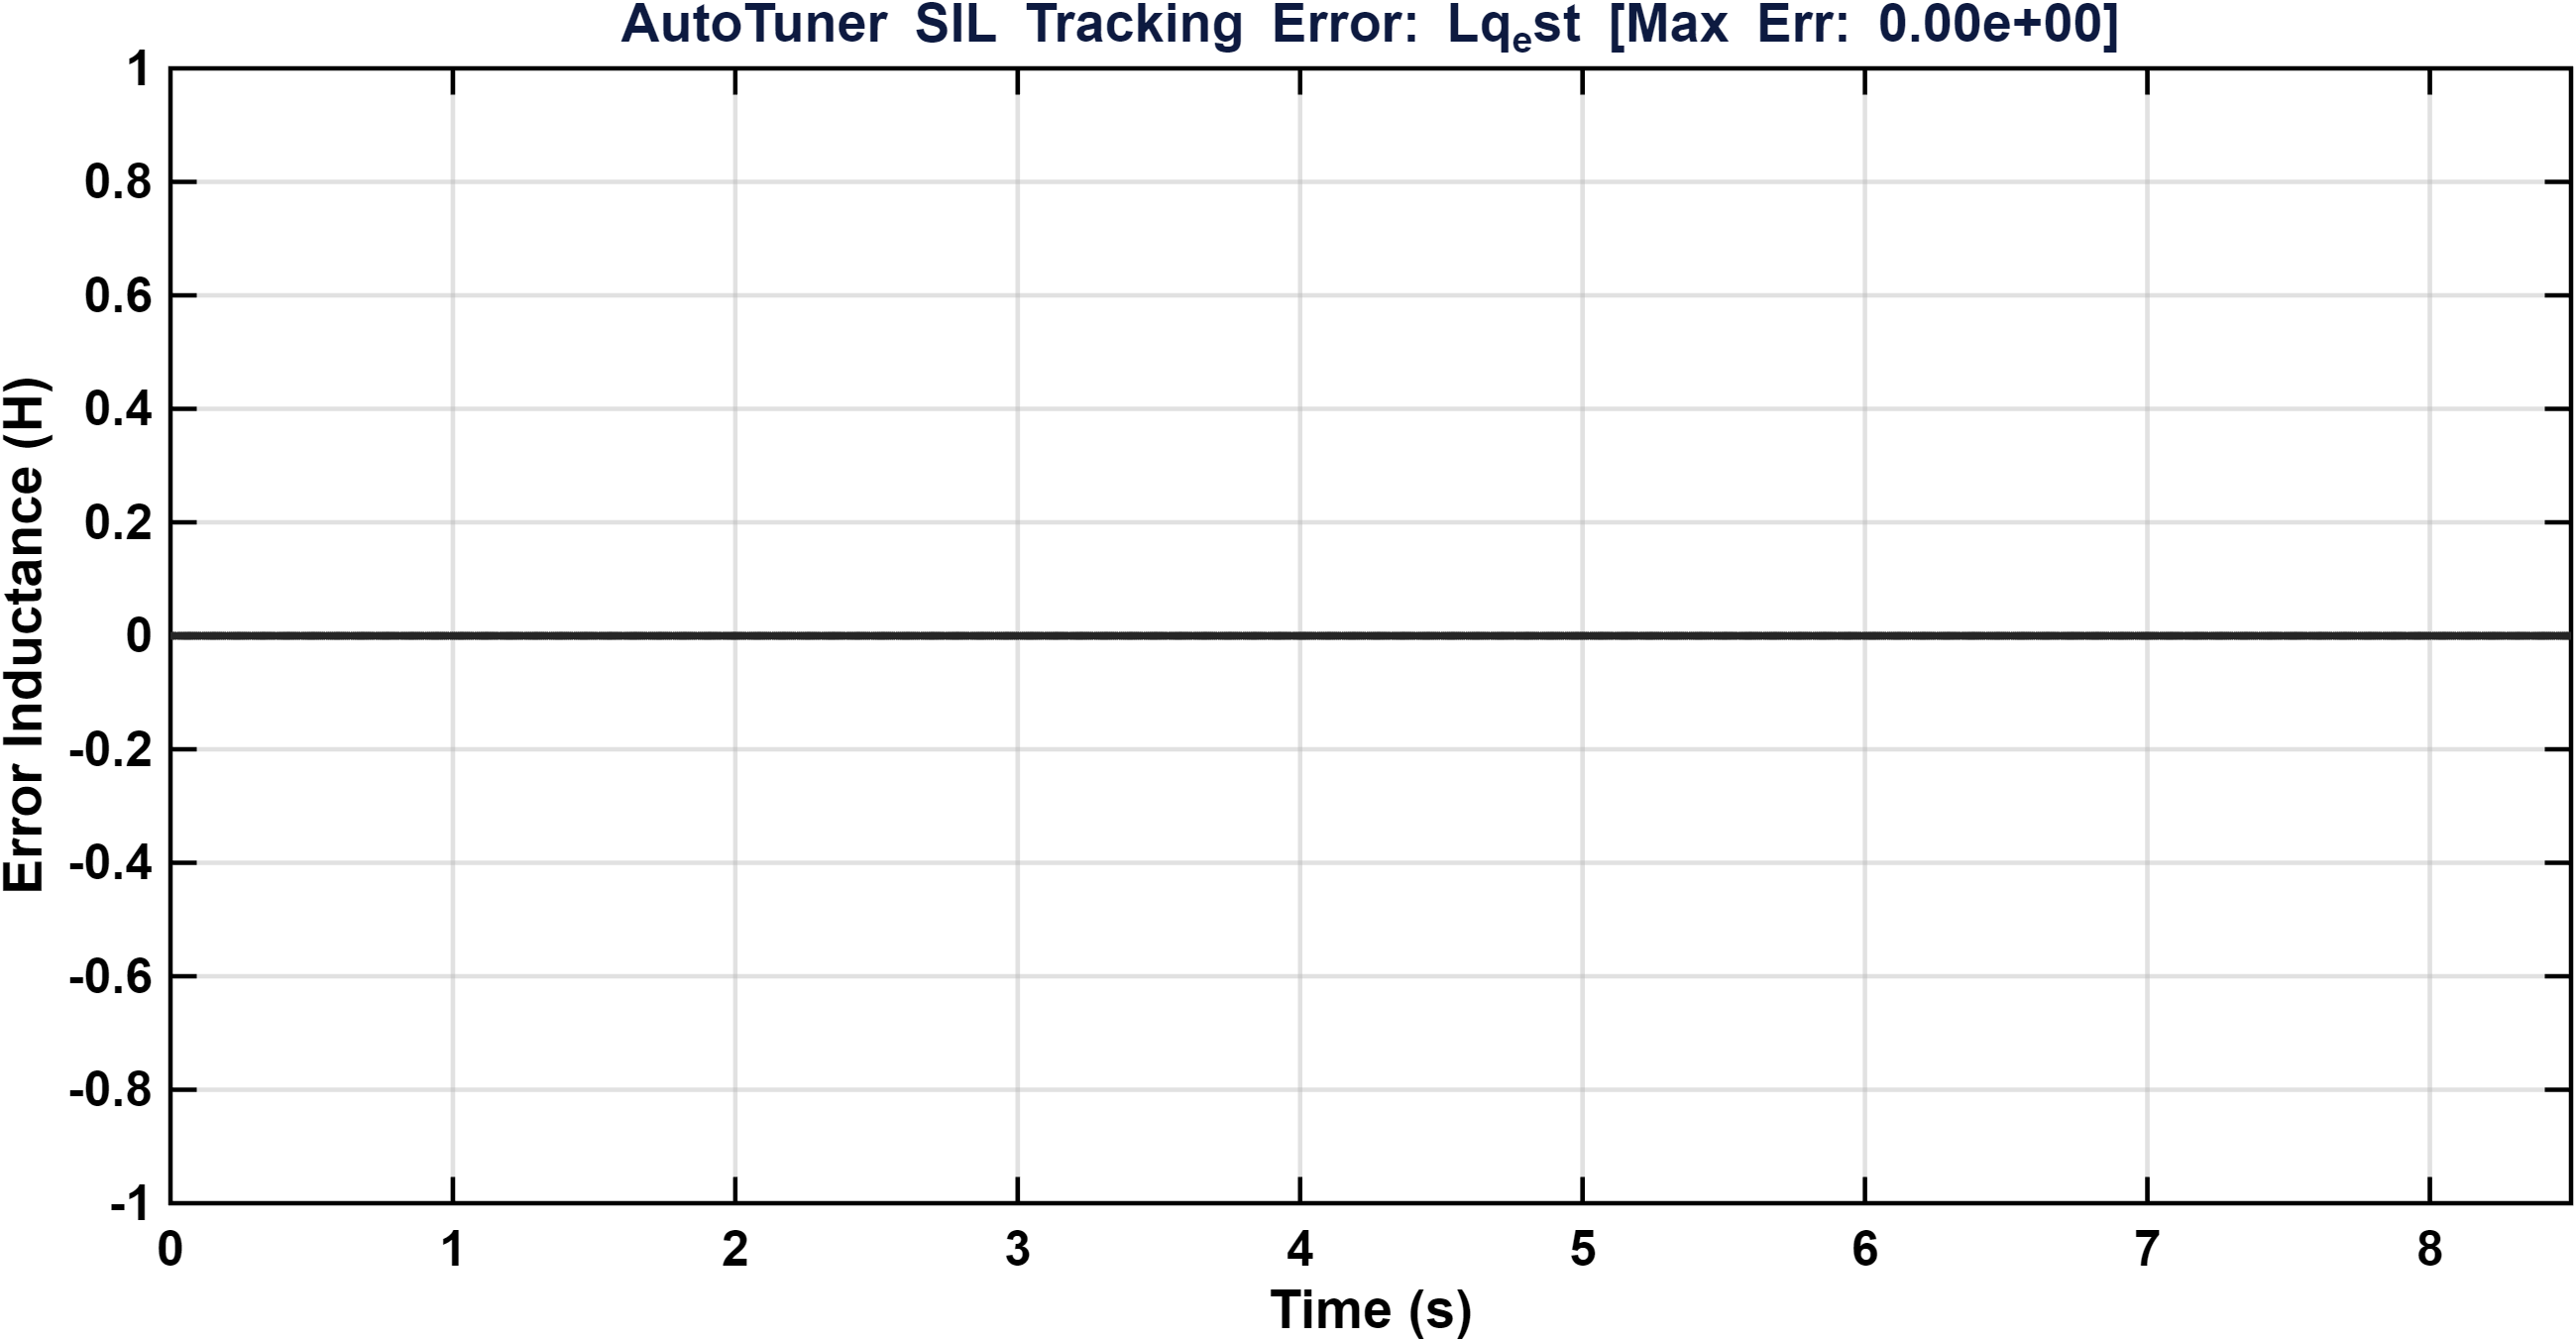
\includegraphics[height=0.52\textheight,keepaspectratio]{AutoTuner_Error_Lq_est.png}
    \vspace{1mm}
    \begin{itemize}
        \footnotesize
        \setlength{\itemsep}{2pt}
        \item \textbf{Error Metric:} Max Absolute Error = \textbf{0.00e+00}.
        \item \textbf{Fidelity:} High-frequency injection logic executes with bit-level parity across host and SIL C-code.
    \end{itemize}
\end{frame}

\begin{frame}{38. AutoTuner Result: PM Flux Linkage ($\Psi_{PM}$) Estimation}
    \centering
    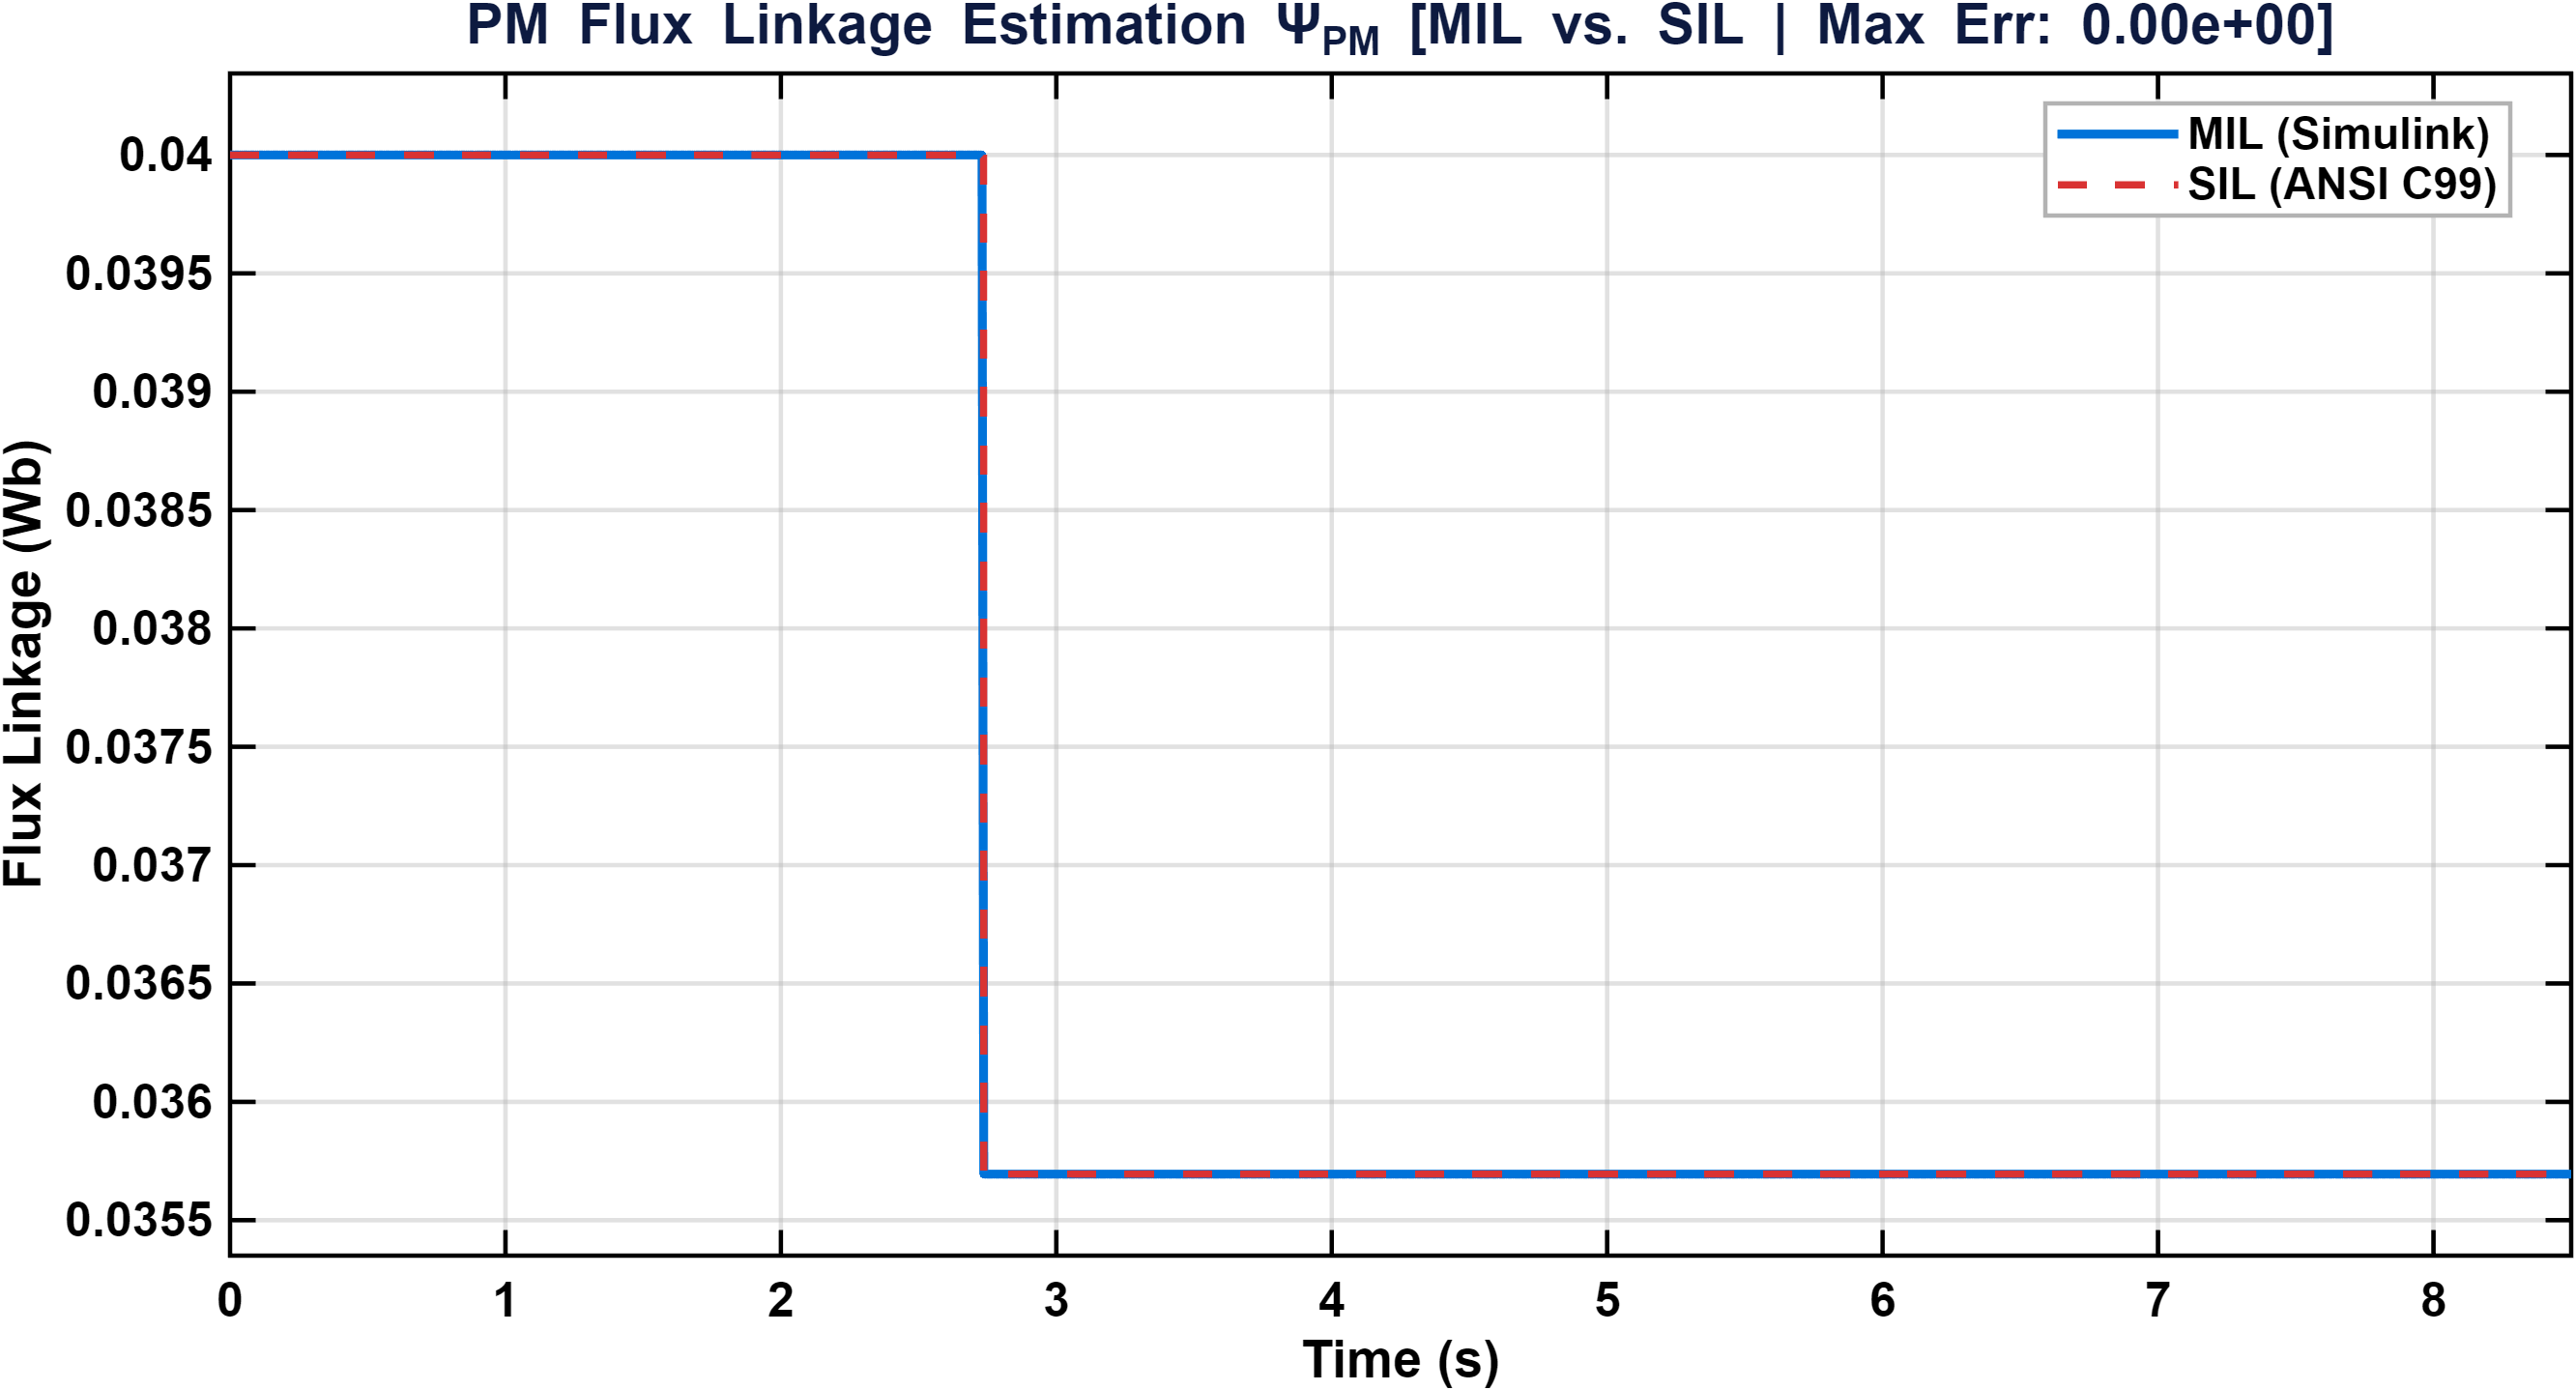
\includegraphics[height=0.52\textheight,keepaspectratio]{AutoTuner_MIL_vs_SIL_PsiPM_est.png}
    \vspace{1mm}
    \begin{itemize}
        \footnotesize
        \setlength{\itemsep}{2pt}
        \item \textbf{Back-EMF Measurement:} Steps from initial guess to identified steady value $\Psi_{PM} = 0.0357\text{ Wb}$ at $t = 3.90\text{ s}$ during unpowered deceleration.
        \item \textbf{Unpowered Safety:} Extraction occurs during zero-current coast-down, eliminating stator resistance offsets.
    \end{itemize}
\end{frame}

\begin{frame}{39. AutoTuner Result: PM Flux Linkage ($\Psi_{PM}$) SIL Error}
    \centering
    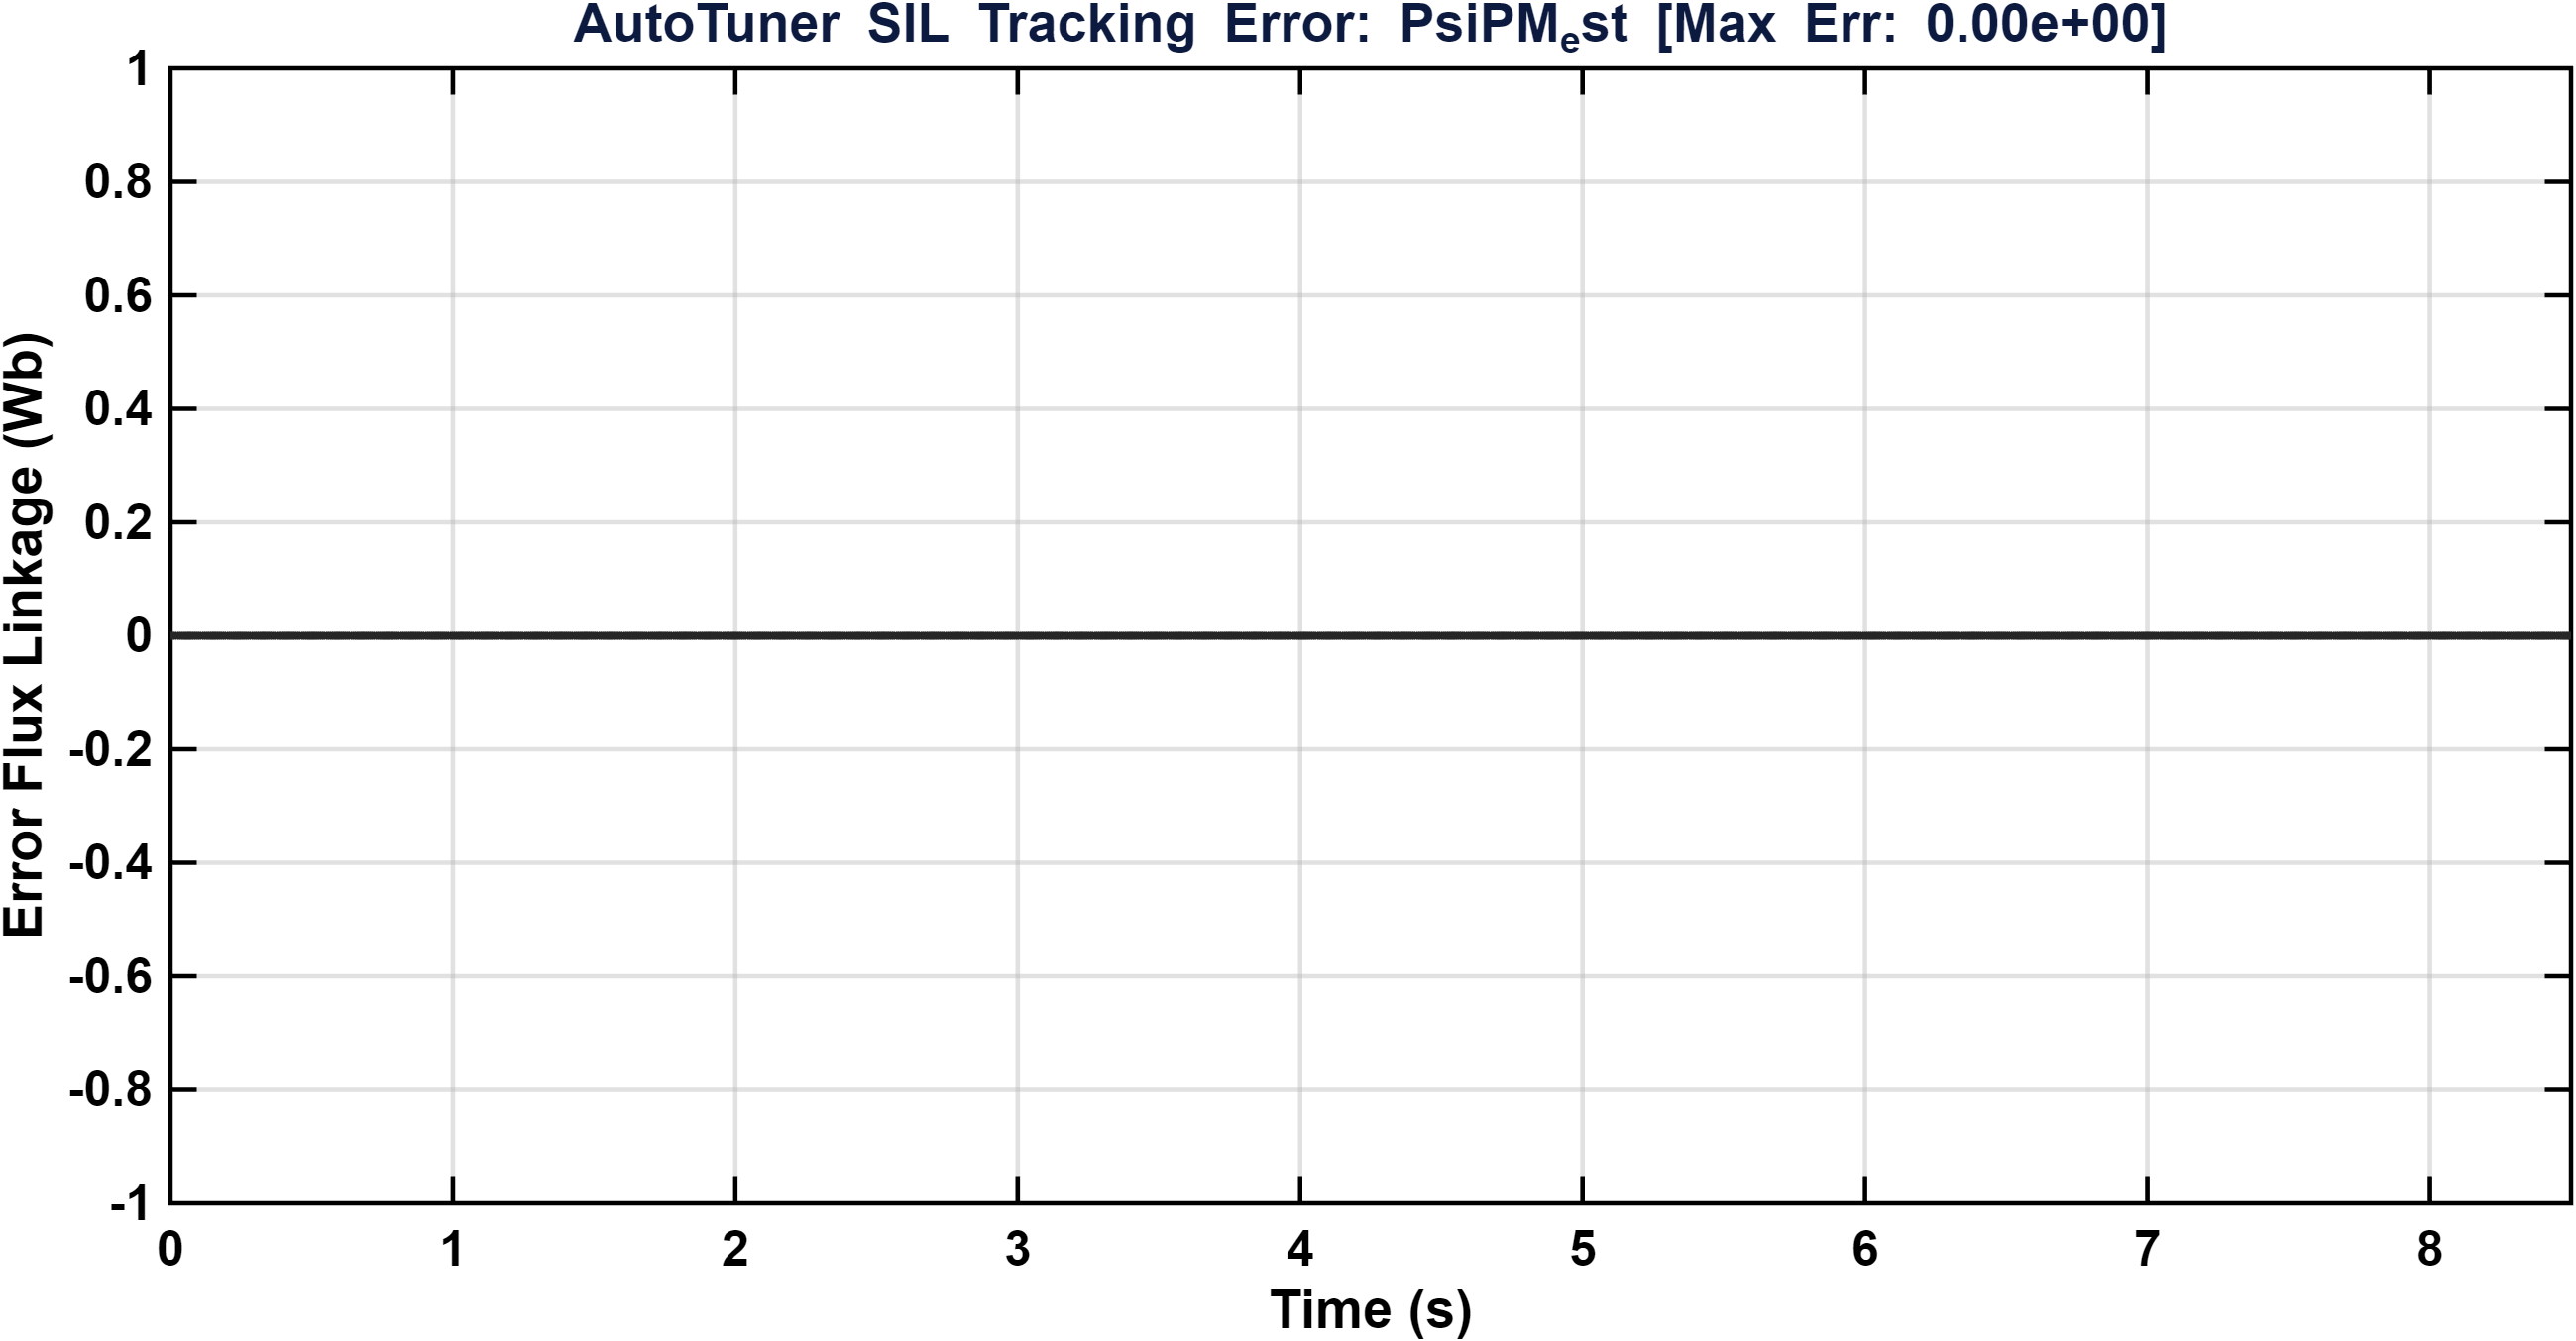
\includegraphics[height=0.52\textheight,keepaspectratio]{AutoTuner_Error_PsiPM_est.png}
    \vspace{1mm}
    \begin{itemize}
        \footnotesize
        \setlength{\itemsep}{2pt}
        \item \textbf{Error Metric:} Max Absolute Error = \textbf{0.00e+00}.
        \item \textbf{Algorithm Fidelity:} Back-EMF moving average filter executes identically in Simulink and generated C-code.
    \end{itemize}
\end{frame}

\begin{frame}{40. AutoTuner Result: Viscous Friction ($B$) Estimation}
    \centering
    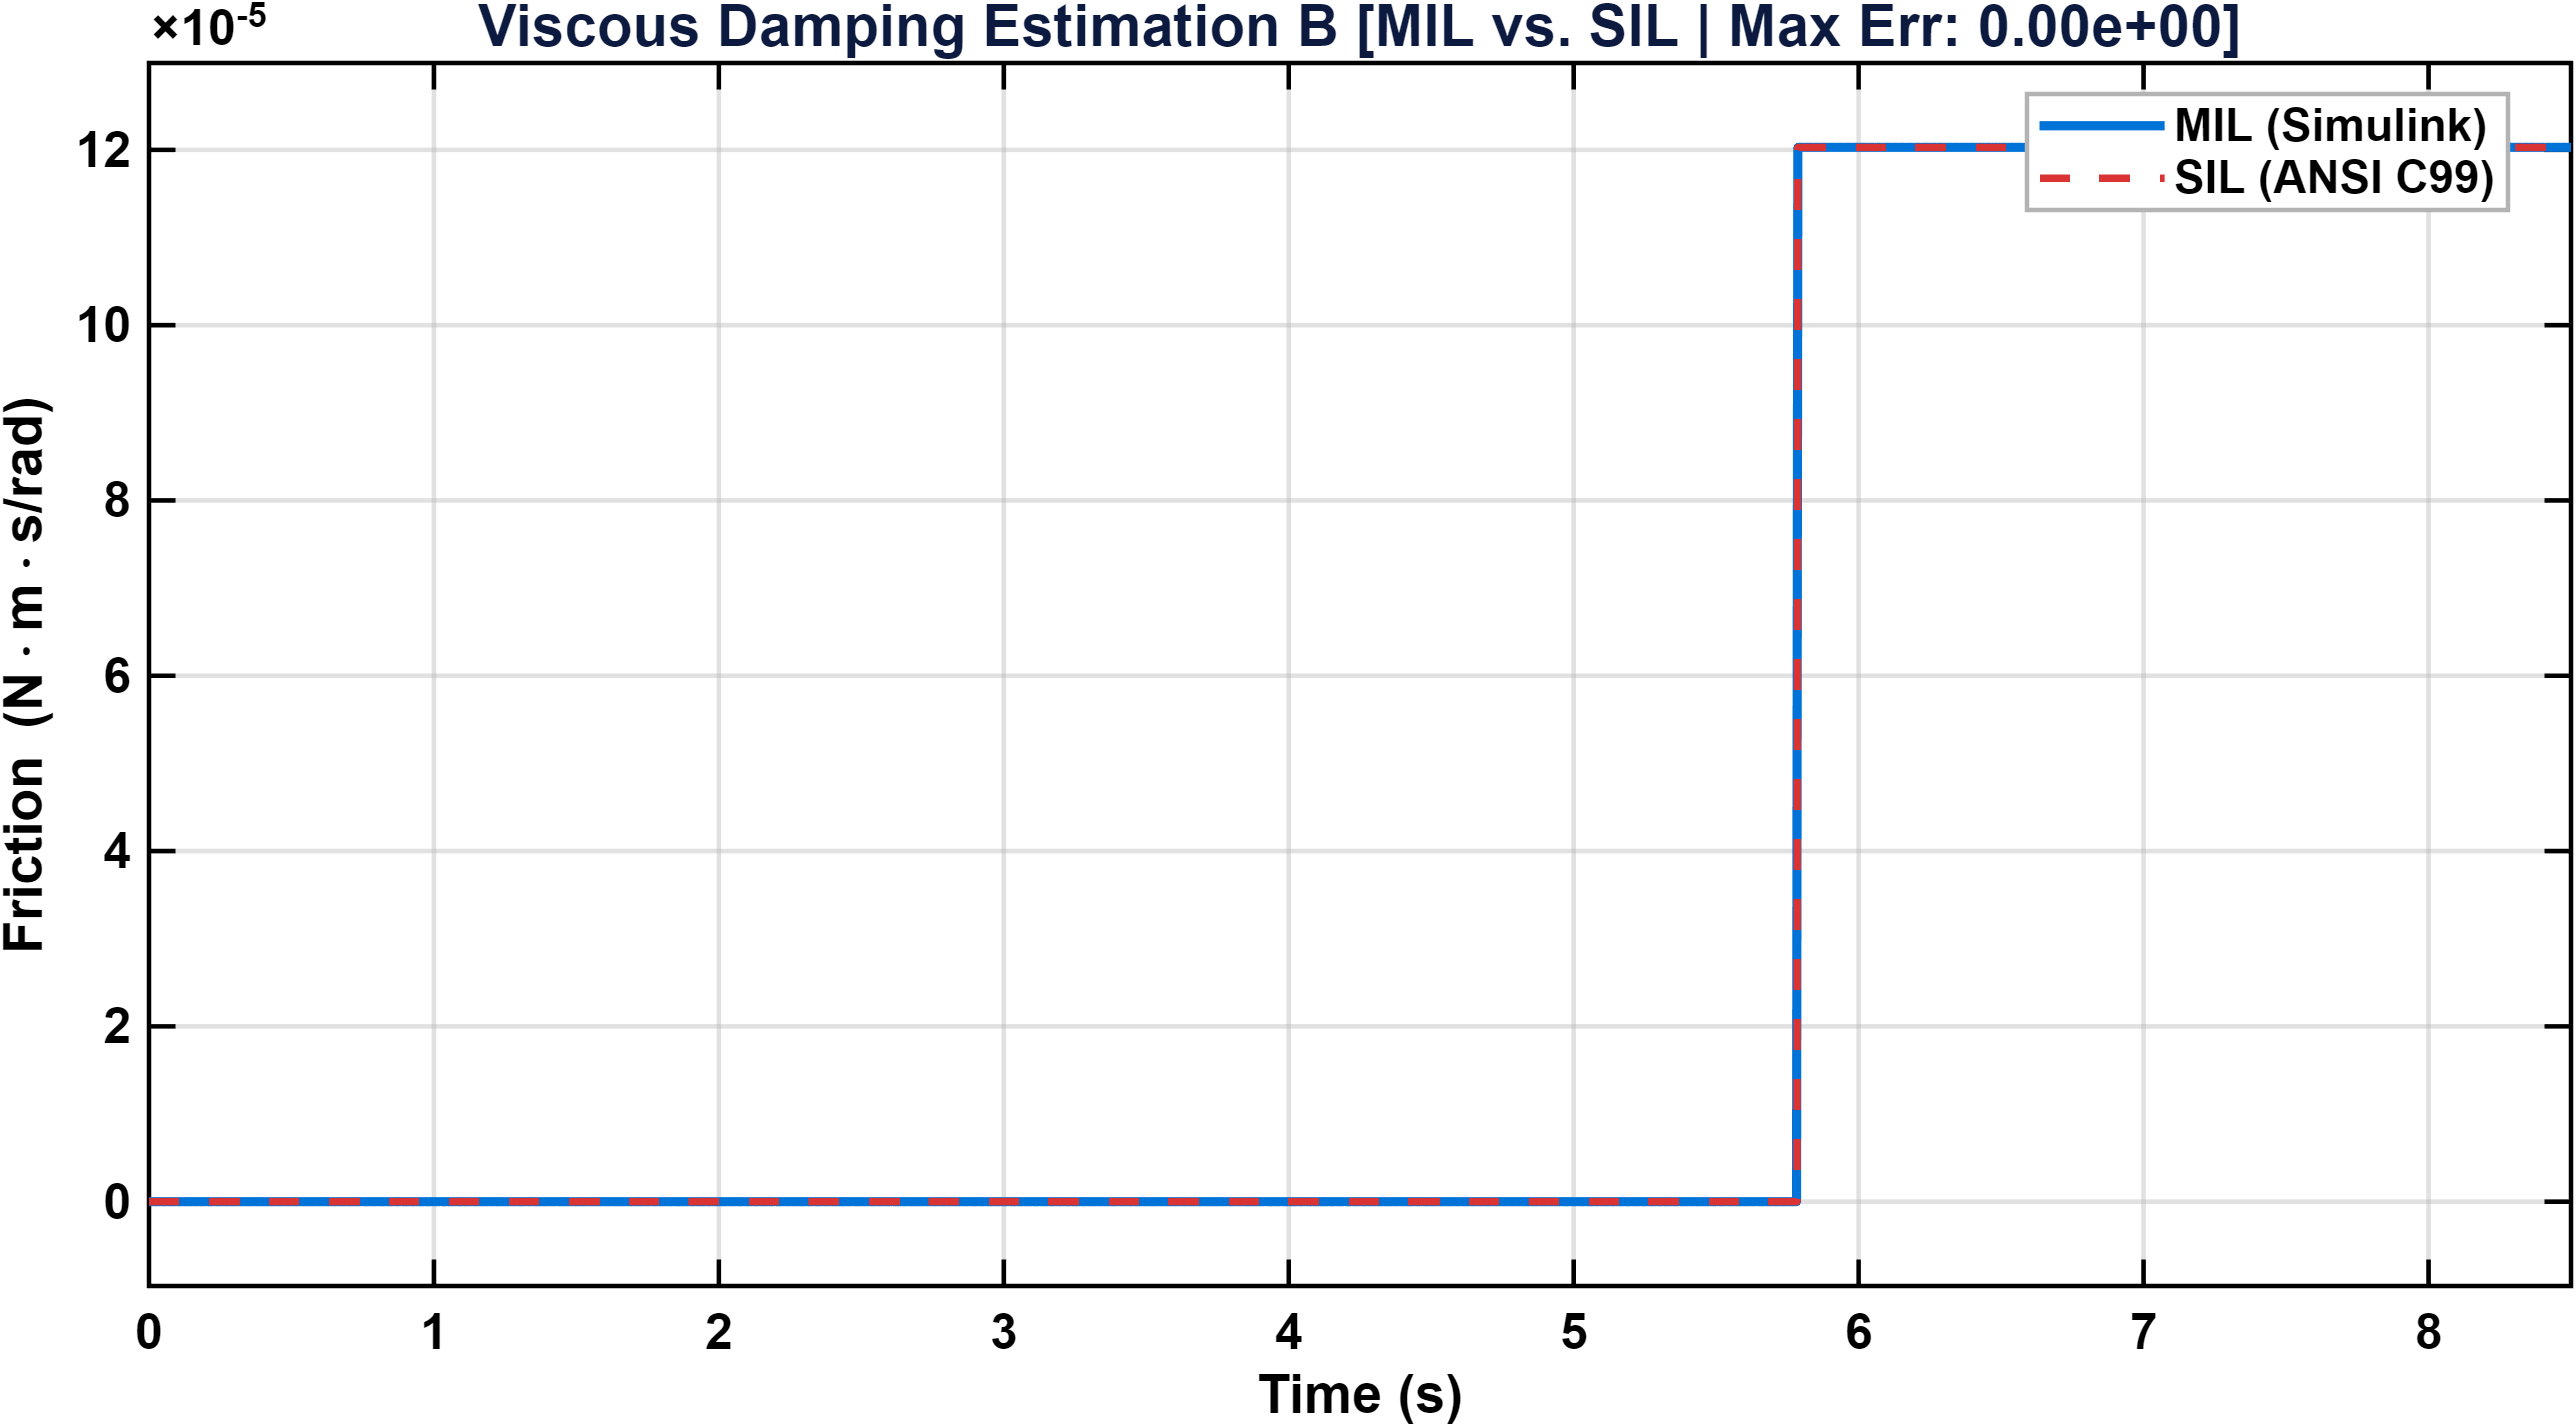
\includegraphics[height=0.52\textheight,keepaspectratio]{AutoTuner_MIL_vs_SIL_B_est.png}
    \vspace{1mm}
    \begin{itemize}
        \footnotesize
        \setlength{\itemsep}{2pt}
        \item \textbf{Two-Point Speed Evaluation:} Steps from 0 to identified $B = 0.00012\text{ N}\cdot\text{m}\cdot\text{s/rad}$ at $t = 6.95\text{ s}$ following the $60\text{ rad/s}$ and $120\text{ rad/s}$ speed holds.
        \item \textbf{Ripple Rejection:} Multi-sample torque averaging completely filters out inverter switching ripple.
    \end{itemize}
\end{frame}

\begin{frame}{41. AutoTuner Result: Viscous Friction ($B$) SIL Error}
    \centering
    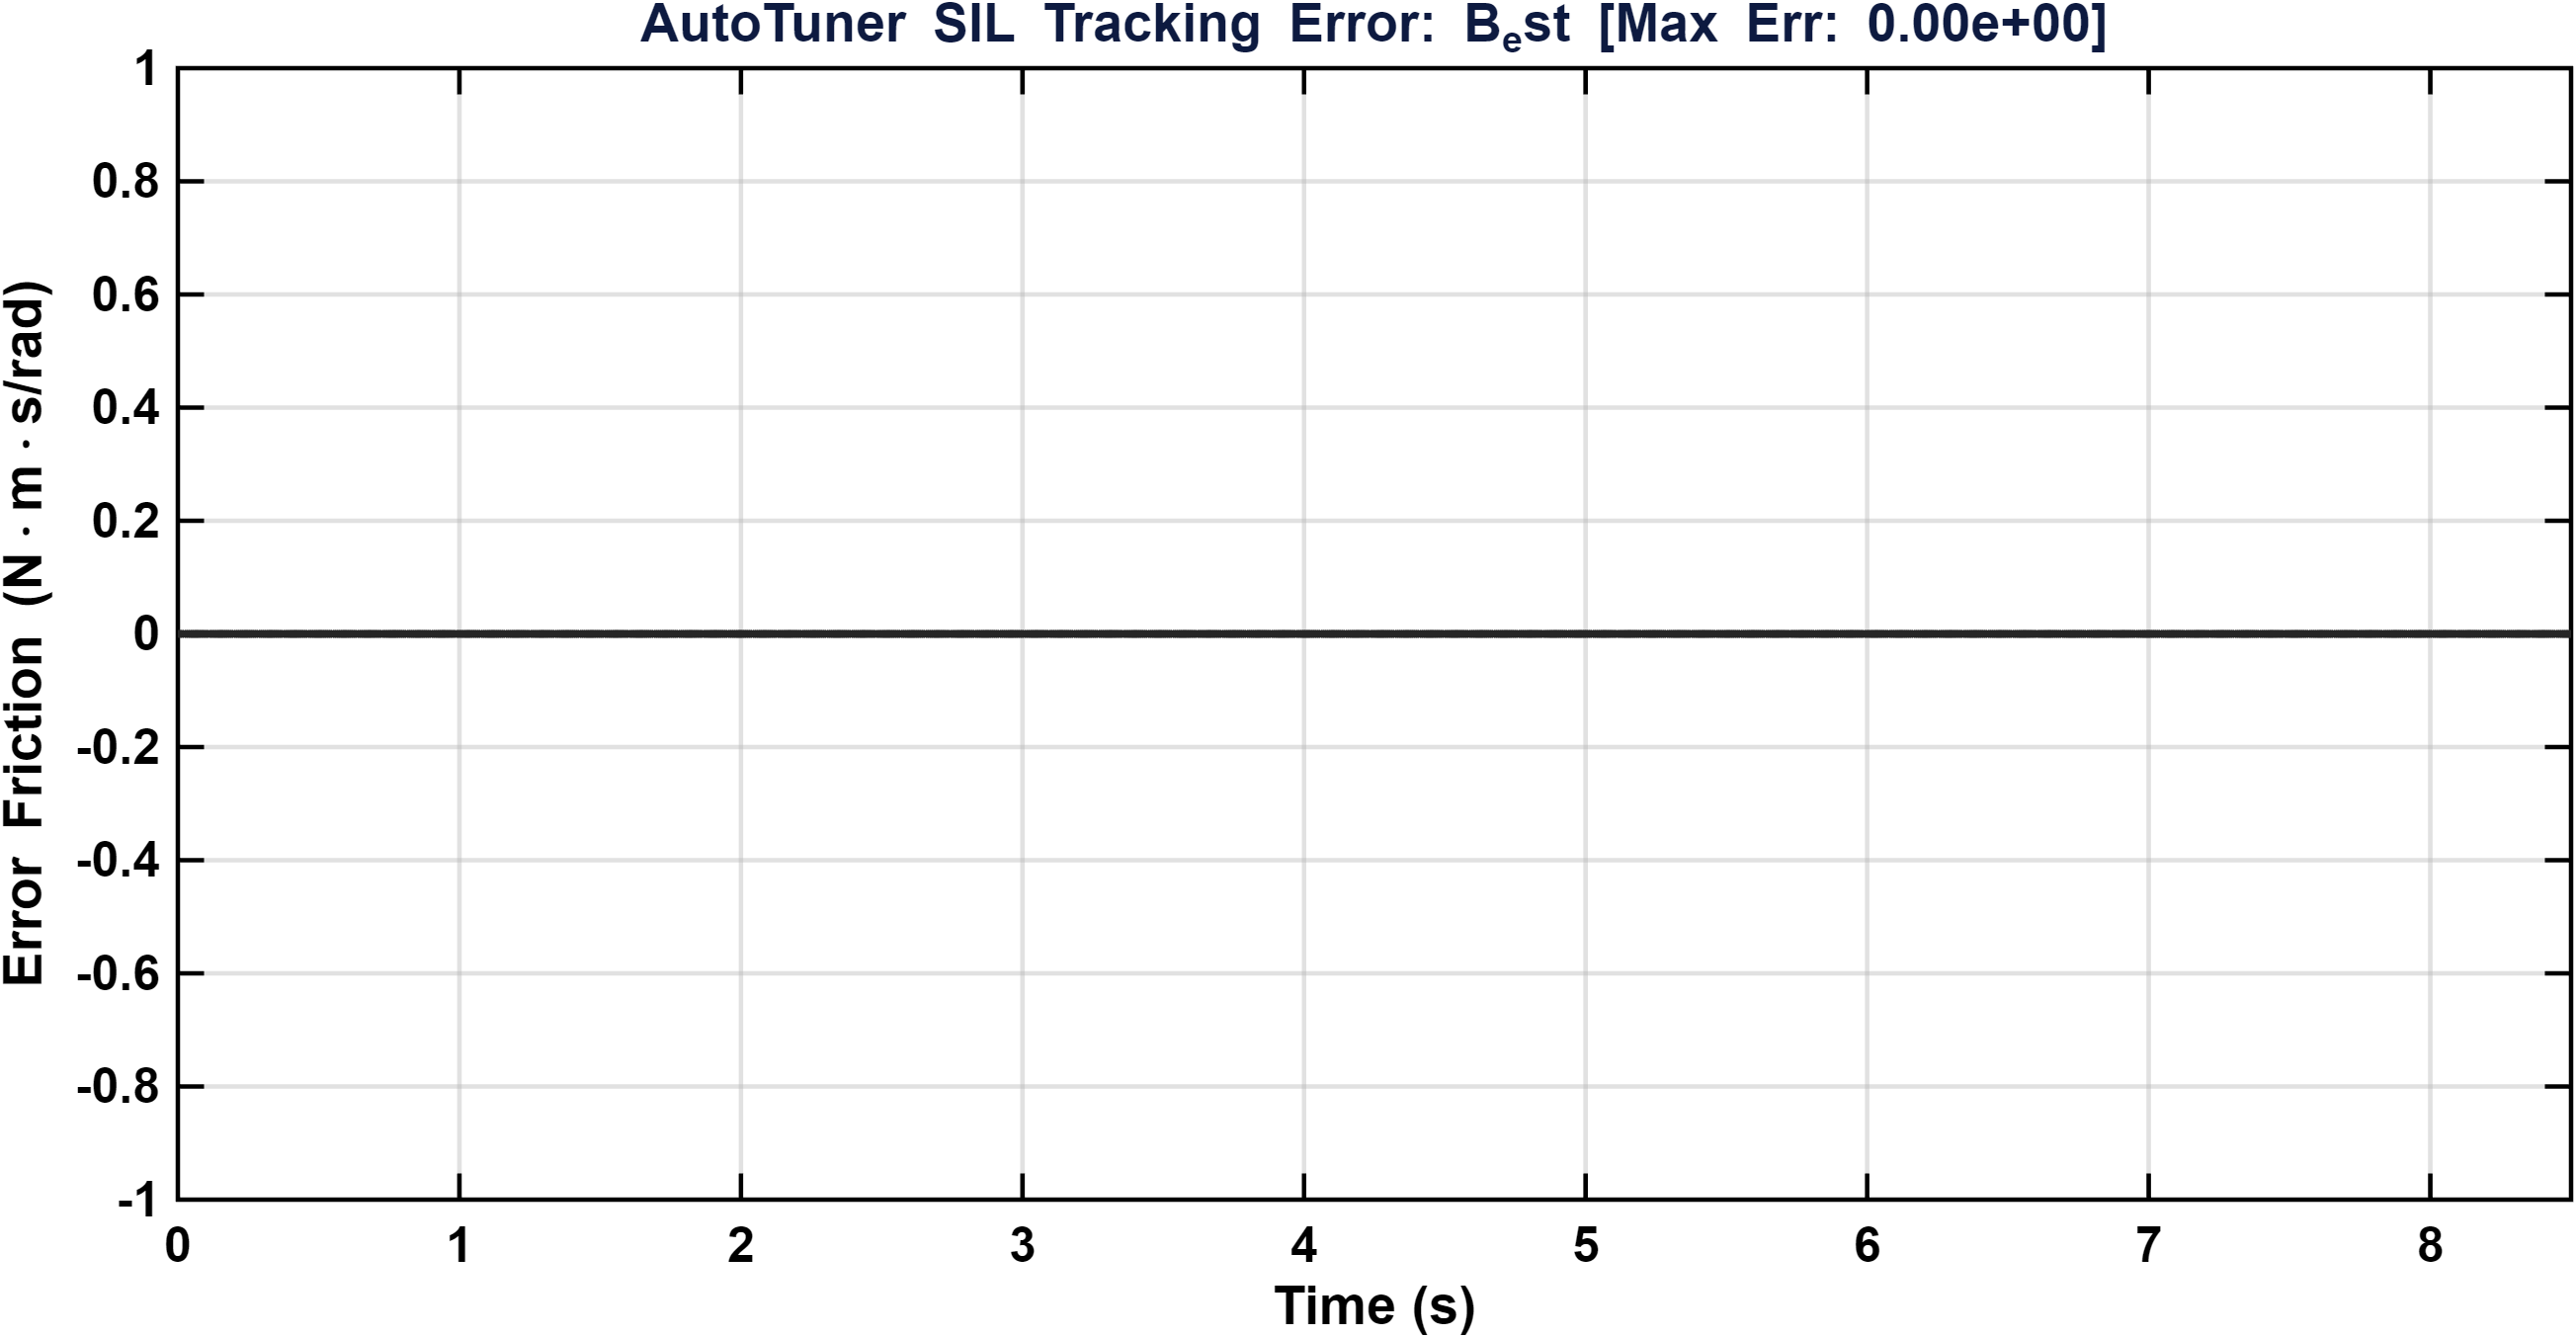
\includegraphics[height=0.52\textheight,keepaspectratio]{AutoTuner_Error_B_est.png}
    \vspace{1mm}
    \begin{itemize}
        \footnotesize
        \setlength{\itemsep}{2pt}
        \item \textbf{Error Metric:} Max Absolute Error = \textbf{0.00e+00}.
        \item \textbf{Robustness:} Identical torque-speed ratio calculations across simulation and target executable.
    \end{itemize}
\end{frame}

\begin{frame}{42. AutoTuner Result: Rotor Inertia ($J$) Estimation}
    \centering
    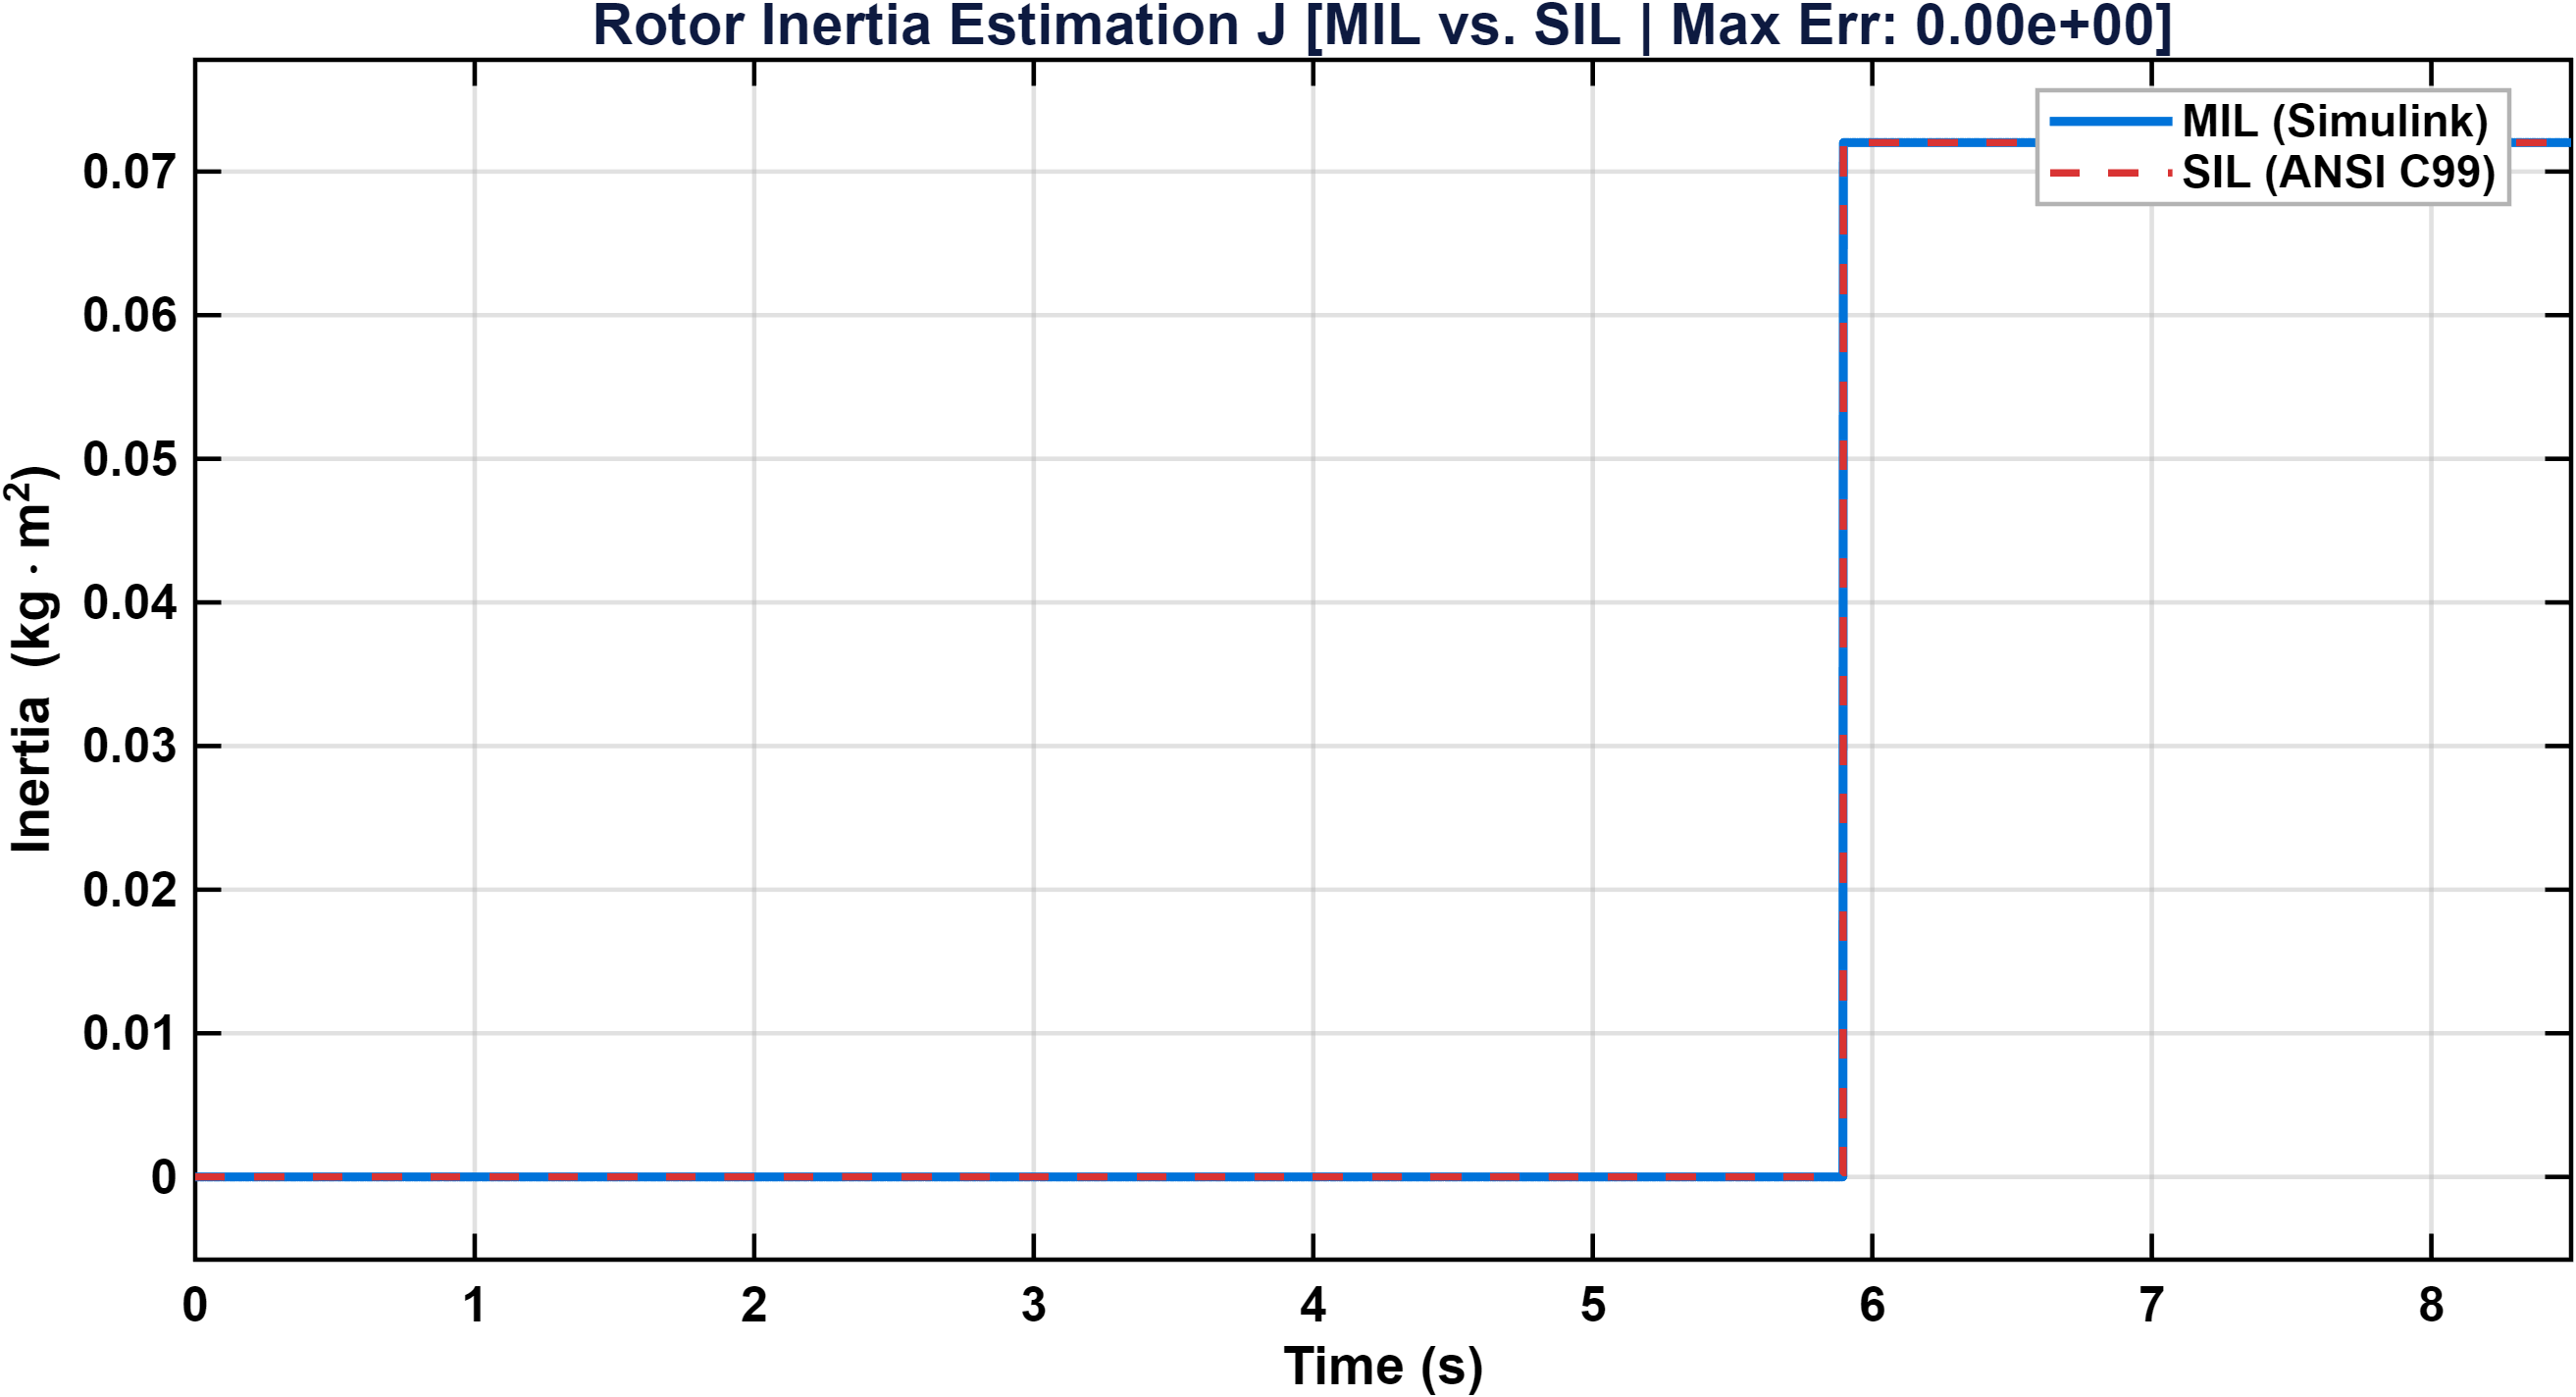
\includegraphics[height=0.52\textheight,keepaspectratio]{AutoTuner_MIL_vs_SIL_J_est.png}
    \vspace{1mm}
    \begin{itemize}
        \footnotesize
        \setlength{\itemsep}{2pt}
        \item \textbf{Active Braking Deceleration Step:} Steps from 0 to identified $J = 0.0720\text{ kg}\cdot\text{m}^2$ at $t = 7.05\text{ s}$ via deceleration rate extraction ($d\omega/dt$).
        \item \textbf{Torque Isolation:} Decouples electromagnetic braking torque from viscous drag cleanly.
    \end{itemize}
\end{frame}

\begin{frame}{43. AutoTuner Result: Rotor Inertia ($J$) SIL Error}
    \centering
    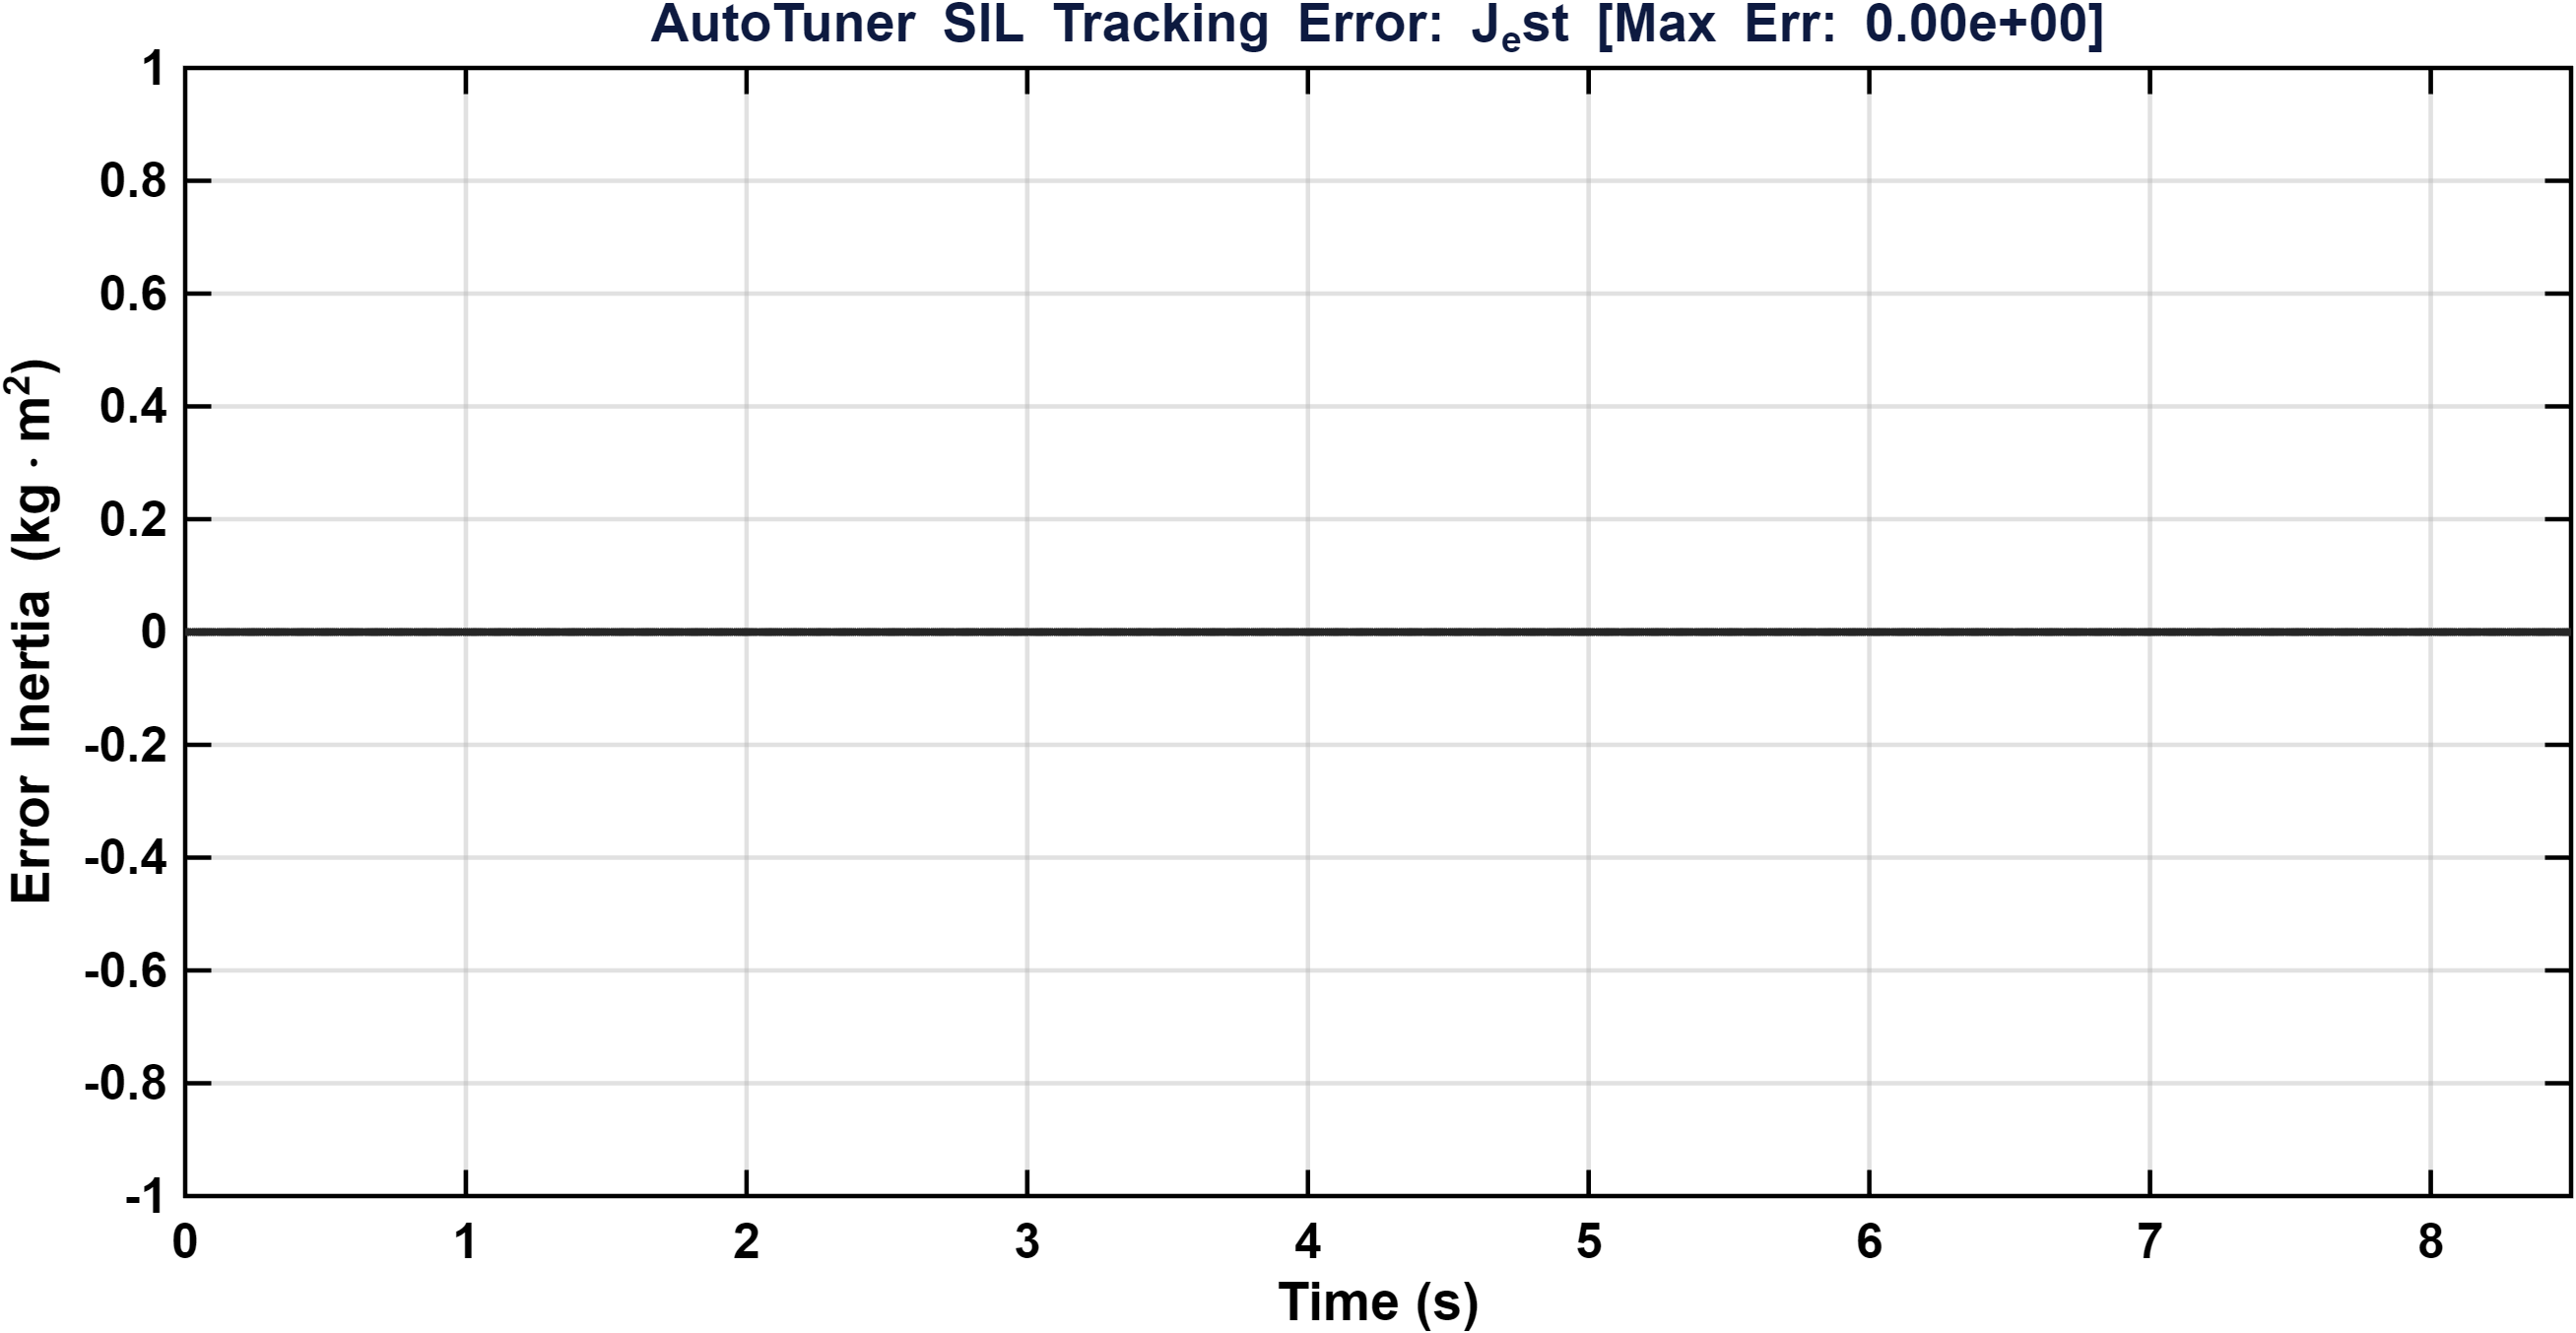
\includegraphics[height=0.52\textheight,keepaspectratio]{AutoTuner_Error_J_est.png}
    \vspace{1mm}
    \begin{itemize}
        \footnotesize
        \setlength{\itemsep}{2pt}
        \item \textbf{Error Metric:} Max Absolute Error = \textbf{0.00e+00}.
        \item \textbf{Timing Precision:} Time integration intervals synchronize perfectly with discrete $10\text{ kHz}$ interrupt ticks.
    \end{itemize}
\end{frame}

\begin{frame}{44. AutoTuner Result: Speed Setpoint Output ($\omega_{ref,out}$)}
    \centering
    
\includegraphics[height=0.52\textheight,keepaspectratio]{AutoTuner_MIL_vs_SIL_omega_ref_out.png}
    \vspace{1mm}
    \begin{itemize}
        \footnotesize
        \setlength{\itemsep}{2pt}
        \item \textbf{Supervisory Trajectory Output:} Holds speed reference at zero during autonomous tuning ($0 - 7.05\text{ s}$), then transparently passes external speed commands ($800\text{ rad/s}$) for $t \ge 7.05\text{ s}$.
        \item \textbf{Anti-Windup Protection:} Integrator gating prevents startup transients upon closed-loop engagement.
    \end{itemize}
\end{frame}

\begin{frame}{45. AutoTuner: Deep Engineering Inferences}
    \begin{itemize}
        \footnotesize
        \setlength{\itemsep}{3pt}
        \item \textbf{Deterministic 7.0-Second Commissioning:}
        \begin{itemize}
            \footnotesize
            \item Comprehensive sequence completes all electrical and mechanical parameter identifications in $7.05\text{ s}$.
            \item Eliminates manual multimeter and dynamometer tests, enabling automated self-commissioning on the production line.
        \end{itemize}
        \item \textbf{Bit-Level Parity Across All Identified Parameters:}
        \begin{itemize}
            \footnotesize
            \item Compiled C code achieves \textbf{0.00e+00} error across all physical parameters ($R_s, L_d, L_q, \Psi_{PM}, J, B$).
            \item Proves zero discretization drift, zero arithmetic rounding bias, and complete single-precision reliability.
        \end{itemize}
        \item \textbf{Dynamic Plug-and-Play Matrix Injection:}
        \begin{itemize}
            \footnotesize
            \item Latching logic automatically populates downstream CCS-MPC state-space matrices ($A_d, B_d$).
            \item Delivers a self-contained, motor-agnostic drive system ready for embedded deployment.
        \end{itemize}
    \end{itemize}
\end{frame}

% ---------------------------------------------------
% SECTION 2: STANDALONE SPEED MPC
% ---------------------------------------------------

\begin{frame}{45a. Standalone Speed MPC Subsystem}
    \centering
    \vspace{4mm}
    \resizebox{0.88\textwidth}{!}{%
    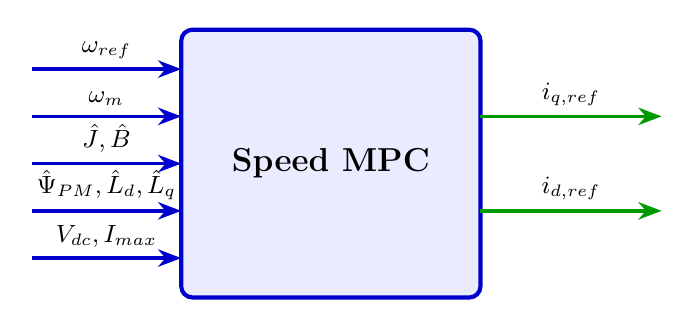
\begin{tikzpicture}[
        block/.style = {rectangle, draw=blue!80!black, line width=1.5pt, fill=blue!8, rounded corners=4pt, align=center, font=\large\bfseries, minimum width=3.8cm, minimum height=3.4cm},
        arr/.style = {->, >=Stealth, line width=1.2pt, draw=blue!80!black},
        outarr/.style = {->, >=Stealth, line width=1.2pt, draw=green!60!black}
    ]
        % Center Block
        \node[block] (sp) at (0, 0) {Speed MPC};

        % Left Inputs (Evenly Spaced)
        \draw[arr] (-3.8,  1.2) -- node[above, font=\small\bfseries] {$\omega_{ref}$} (-1.9,  1.2);
        \draw[arr] (-3.8,  0.6) -- node[above, font=\small\bfseries] {$\omega_m$} (-1.9,  0.6);
        \draw[arr] (-3.8,  0.0) -- node[above, font=\small\bfseries] {$\hat{J}, \hat{B}$} (-1.9,  0.0);
        \draw[arr] (-3.8, -0.6) -- node[above, font=\small\bfseries] {$\hat{\Psi}_{PM}, \hat{L}_d, \hat{L}_q$} (-1.9, -0.6);
        \draw[arr] (-3.8, -1.2) -- node[above, font=\small\bfseries] {$V_{dc}, I_{max}$} (-1.9, -1.2);

        % Right Outputs (Evenly Spaced)
        \draw[outarr] (1.9,  0.6) -- node[above, font=\small\bfseries] {$i_{q,ref}$} (4.2,  0.6);
        \draw[outarr] (1.9, -0.6) -- node[above, font=\small\bfseries] {$i_{d,ref}$} (4.2, -0.6);

    \end{tikzpicture}%
    }
    \vspace{6mm}
    \begin{itemize}
        \small
        \item \textbf{Subsystem Function:} Regulates motor mechanical speed using state-space prediction and synthesizes optimal torque ($i_{q,ref}$) and flux-weakening ($i_{d,ref}$) current commands.
    \end{itemize}
\end{frame}

\begin{frame}{46. Speed MPC: Mechanical State-Space Dynamics}
    \begin{itemize}
        \footnotesize
        \setlength{\itemsep}{2pt}
        \item \textbf{Continuous Mechanical Plant Dynamics:}
        \begin{equation}
            \frac{d\omega_m}{dt} = \frac{T_e - T_L - B\omega_m}{J} = \frac{\frac{3}{2} p \left[ \Psi_{PM} i_q + (L_d - L_q) i_d i_q \right] - T_L - B\omega_m}{J}
        \end{equation}
        \item \textbf{Forward Euler Discrete State-Space Formulation ($T_s = 100\ \mu\text{s}$):}
        \begin{equation}
            \omega_m(k+1) = \left(1 - \frac{T_s \hat{B}}{\hat{J}}\right) \omega_m(k) + \frac{T_s K_t}{\hat{J}} i_q(k) - \frac{T_s}{\hat{J}} T_L(k)
        \end{equation}
        \item \textbf{Analytical Deadbeat Torque Command ($\frac{\partial J_{cost}}{\partial i_q} = 0$):}
        \begin{equation}
            i_{q,ref}(k) = \text{sat}\left( \frac{\hat{J}}{T_s K_t} \left[ \omega_{ref}(k+1) - \left(1 - \frac{T_s \hat{B}}{\hat{J}}\right)\omega_m(k) \right], \pm I_{max} \right)
        \end{equation}
    \end{itemize}
\end{frame}

\begin{frame}{47. Speed MPC Result: Speed Tracking Profile ($\omega_e$)}
    \centering
    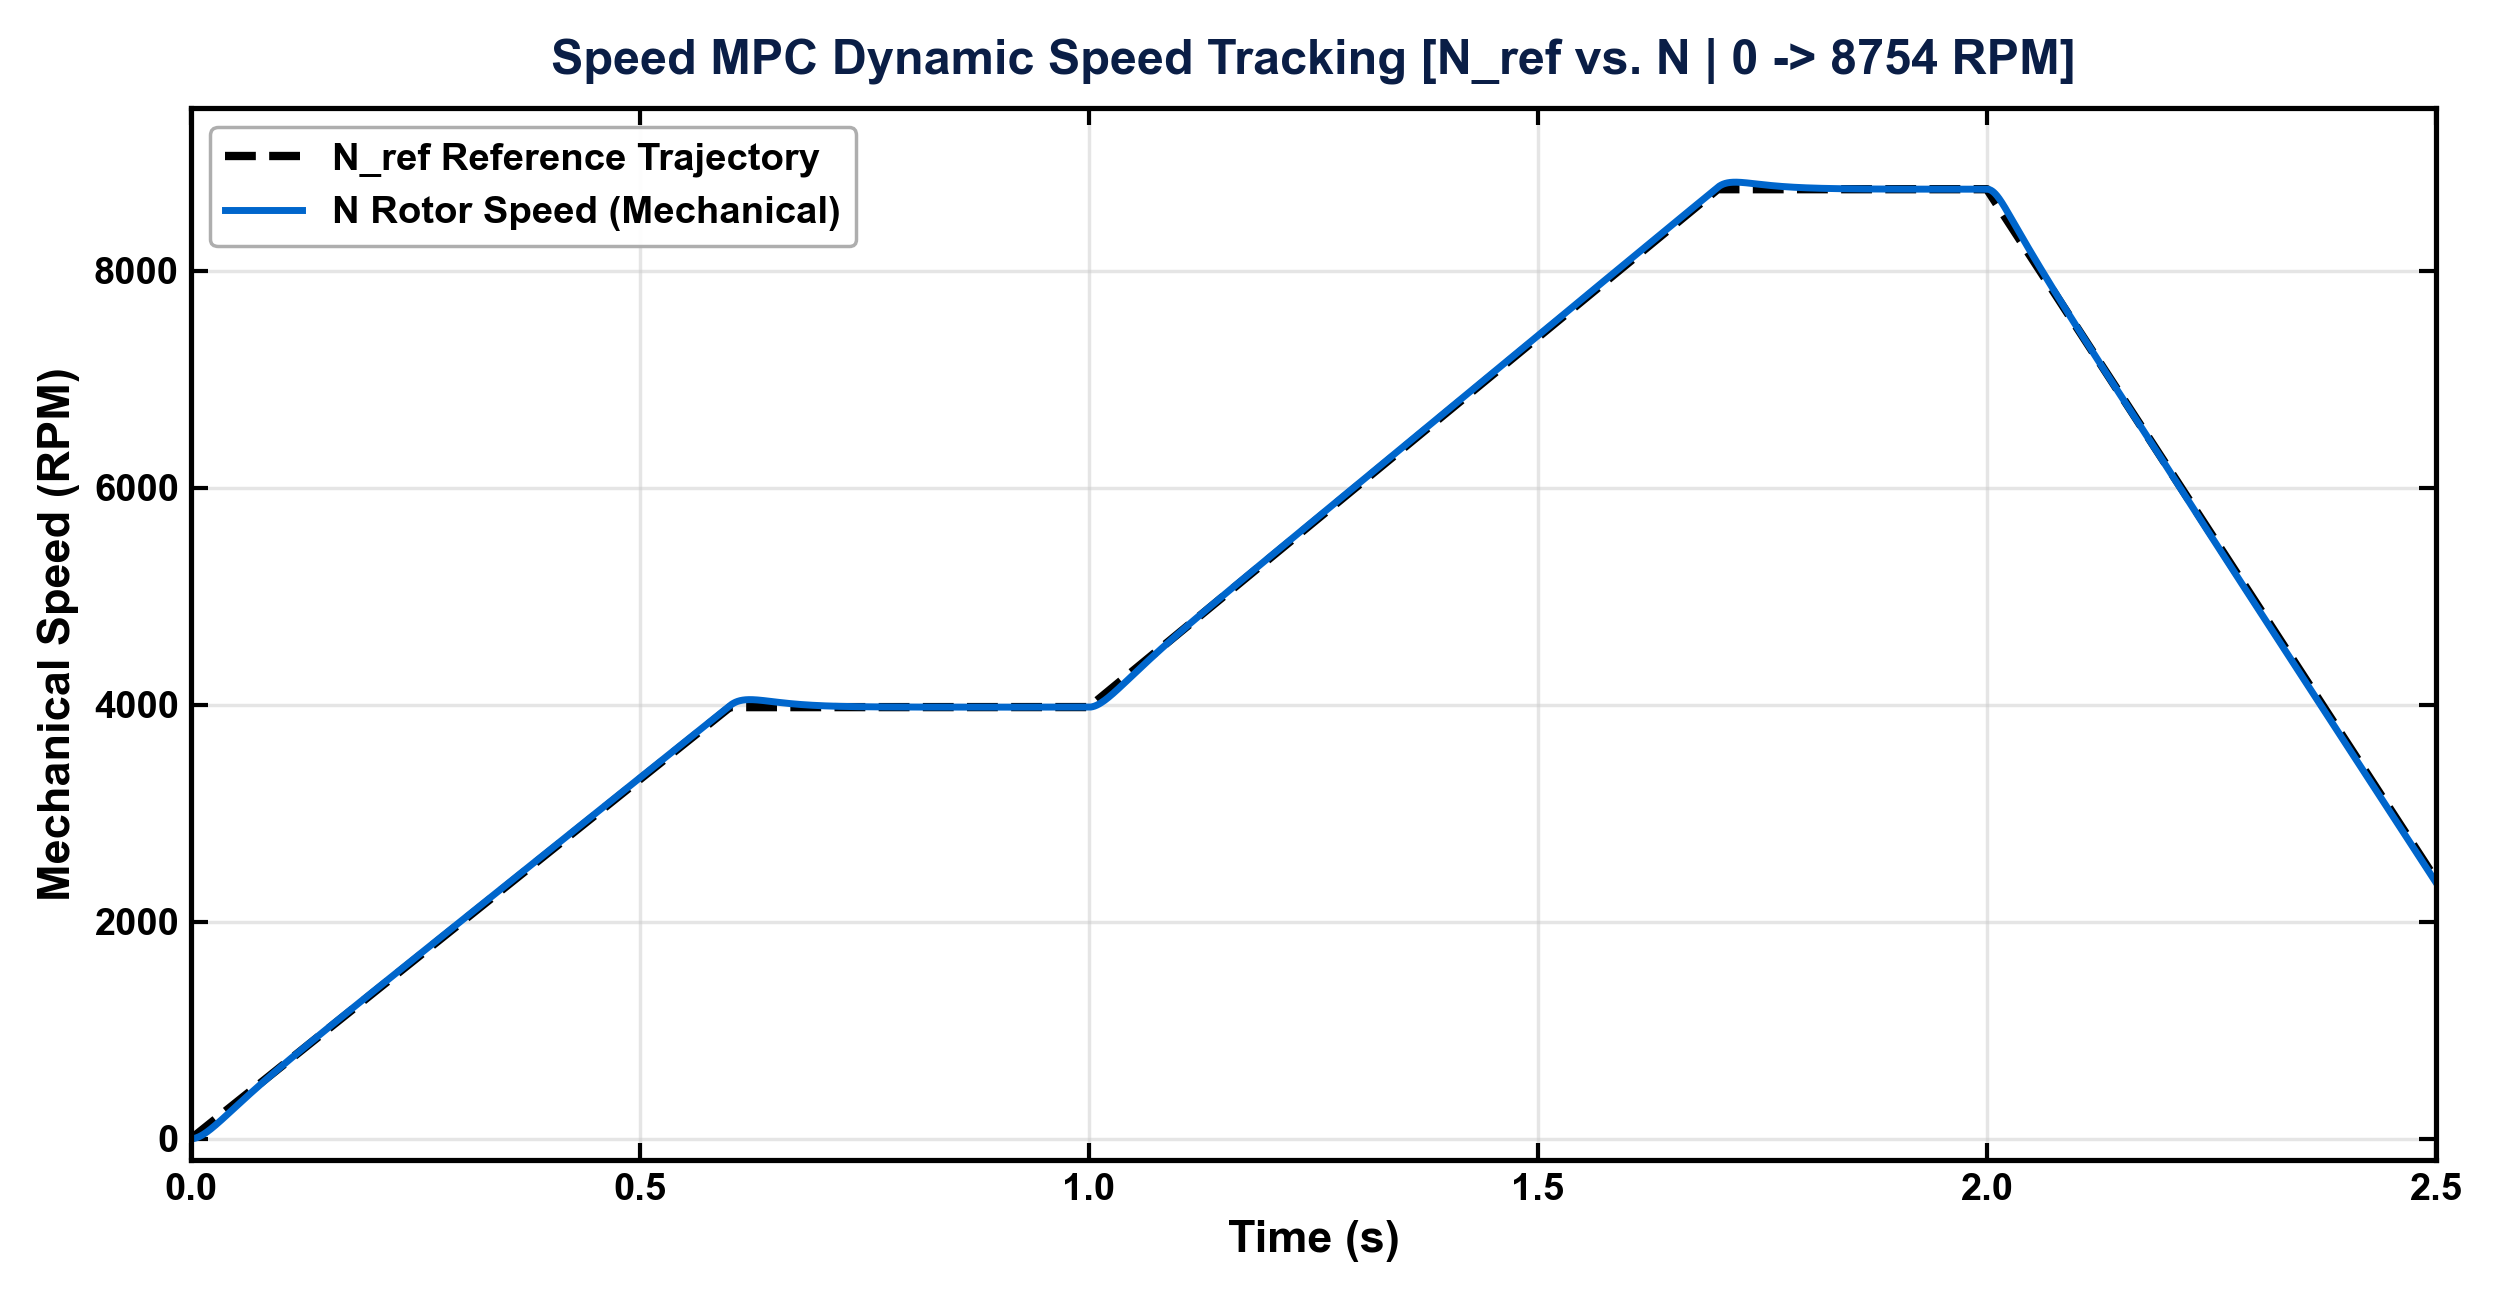
\includegraphics[height=0.52\textheight,keepaspectratio]{Speed_MPC_Tracking_Speed.png}
    \vspace{1mm}
    \begin{itemize}
        \footnotesize
        \setlength{\itemsep}{2pt}
        \item \textbf{Multi-Regime Speed Trajectory ($0 - 2.5\text{ s}$ Electrical Rad/s Timeline):} Base speed MTPA ramp ($0 \rightarrow 2500\text{ rad/s}$ electrical $\equiv 3979\text{ RPM}$ at $t=0.6\text{ s}$), field-weakening acceleration ($2500 \rightarrow 5500\text{ rad/s} \equiv 8754\text{ RPM}$ at $t=1.7\text{ s}$), and regenerative braking ($5500 \rightarrow 1500\text{ rad/s} \equiv 2387\text{ RPM}$ at $t=2.5\text{ s}$).
        \item \textbf{Tracking Precision:} Actual rotor speed $\omega_e$ (solid blue) tracks reference $\omega_{ref}$ (dashed black) with high dynamic fidelity and zero overshoot.
    \end{itemize}
\end{frame}

\begin{frame}{48. Speed MPC Result: Speed Tracking Error ($e_\omega = \omega_{ref} - \omega_e$)}
    \centering
    
\includegraphics[height=0.52\textheight,keepaspectratio]{Speed_MPC_Tracking_Error_Speed.png}
    \vspace{1mm}
    \begin{itemize}
        \footnotesize
        \setlength{\itemsep}{2pt}
        \item \textbf{Transient Error Dynamics ($0 - 2.5\text{ s}$):} Error peaks briefly ($\approx 54.5\text{ rad/s} \equiv 86.7\text{ RPM}$) during steep acceleration transitions ($4166\text{ rad/s}^2$), then settles cleanly to \textbf{$< 0.03\text{ rad/s}$ ($< 0.045\text{ RPM}$)} in steady state.
        \item \textbf{Dynamic Stiffness:} Properly weighted cost function ($K_{p}=6.5, K_{i}=120.0$) eliminates derivative chattering and suppresses friction load droop.
    \end{itemize}
\end{frame}

\begin{frame}{49. Speed MPC Result: Torque Reference Current ($i_{q,ref}$)}
    \centering
    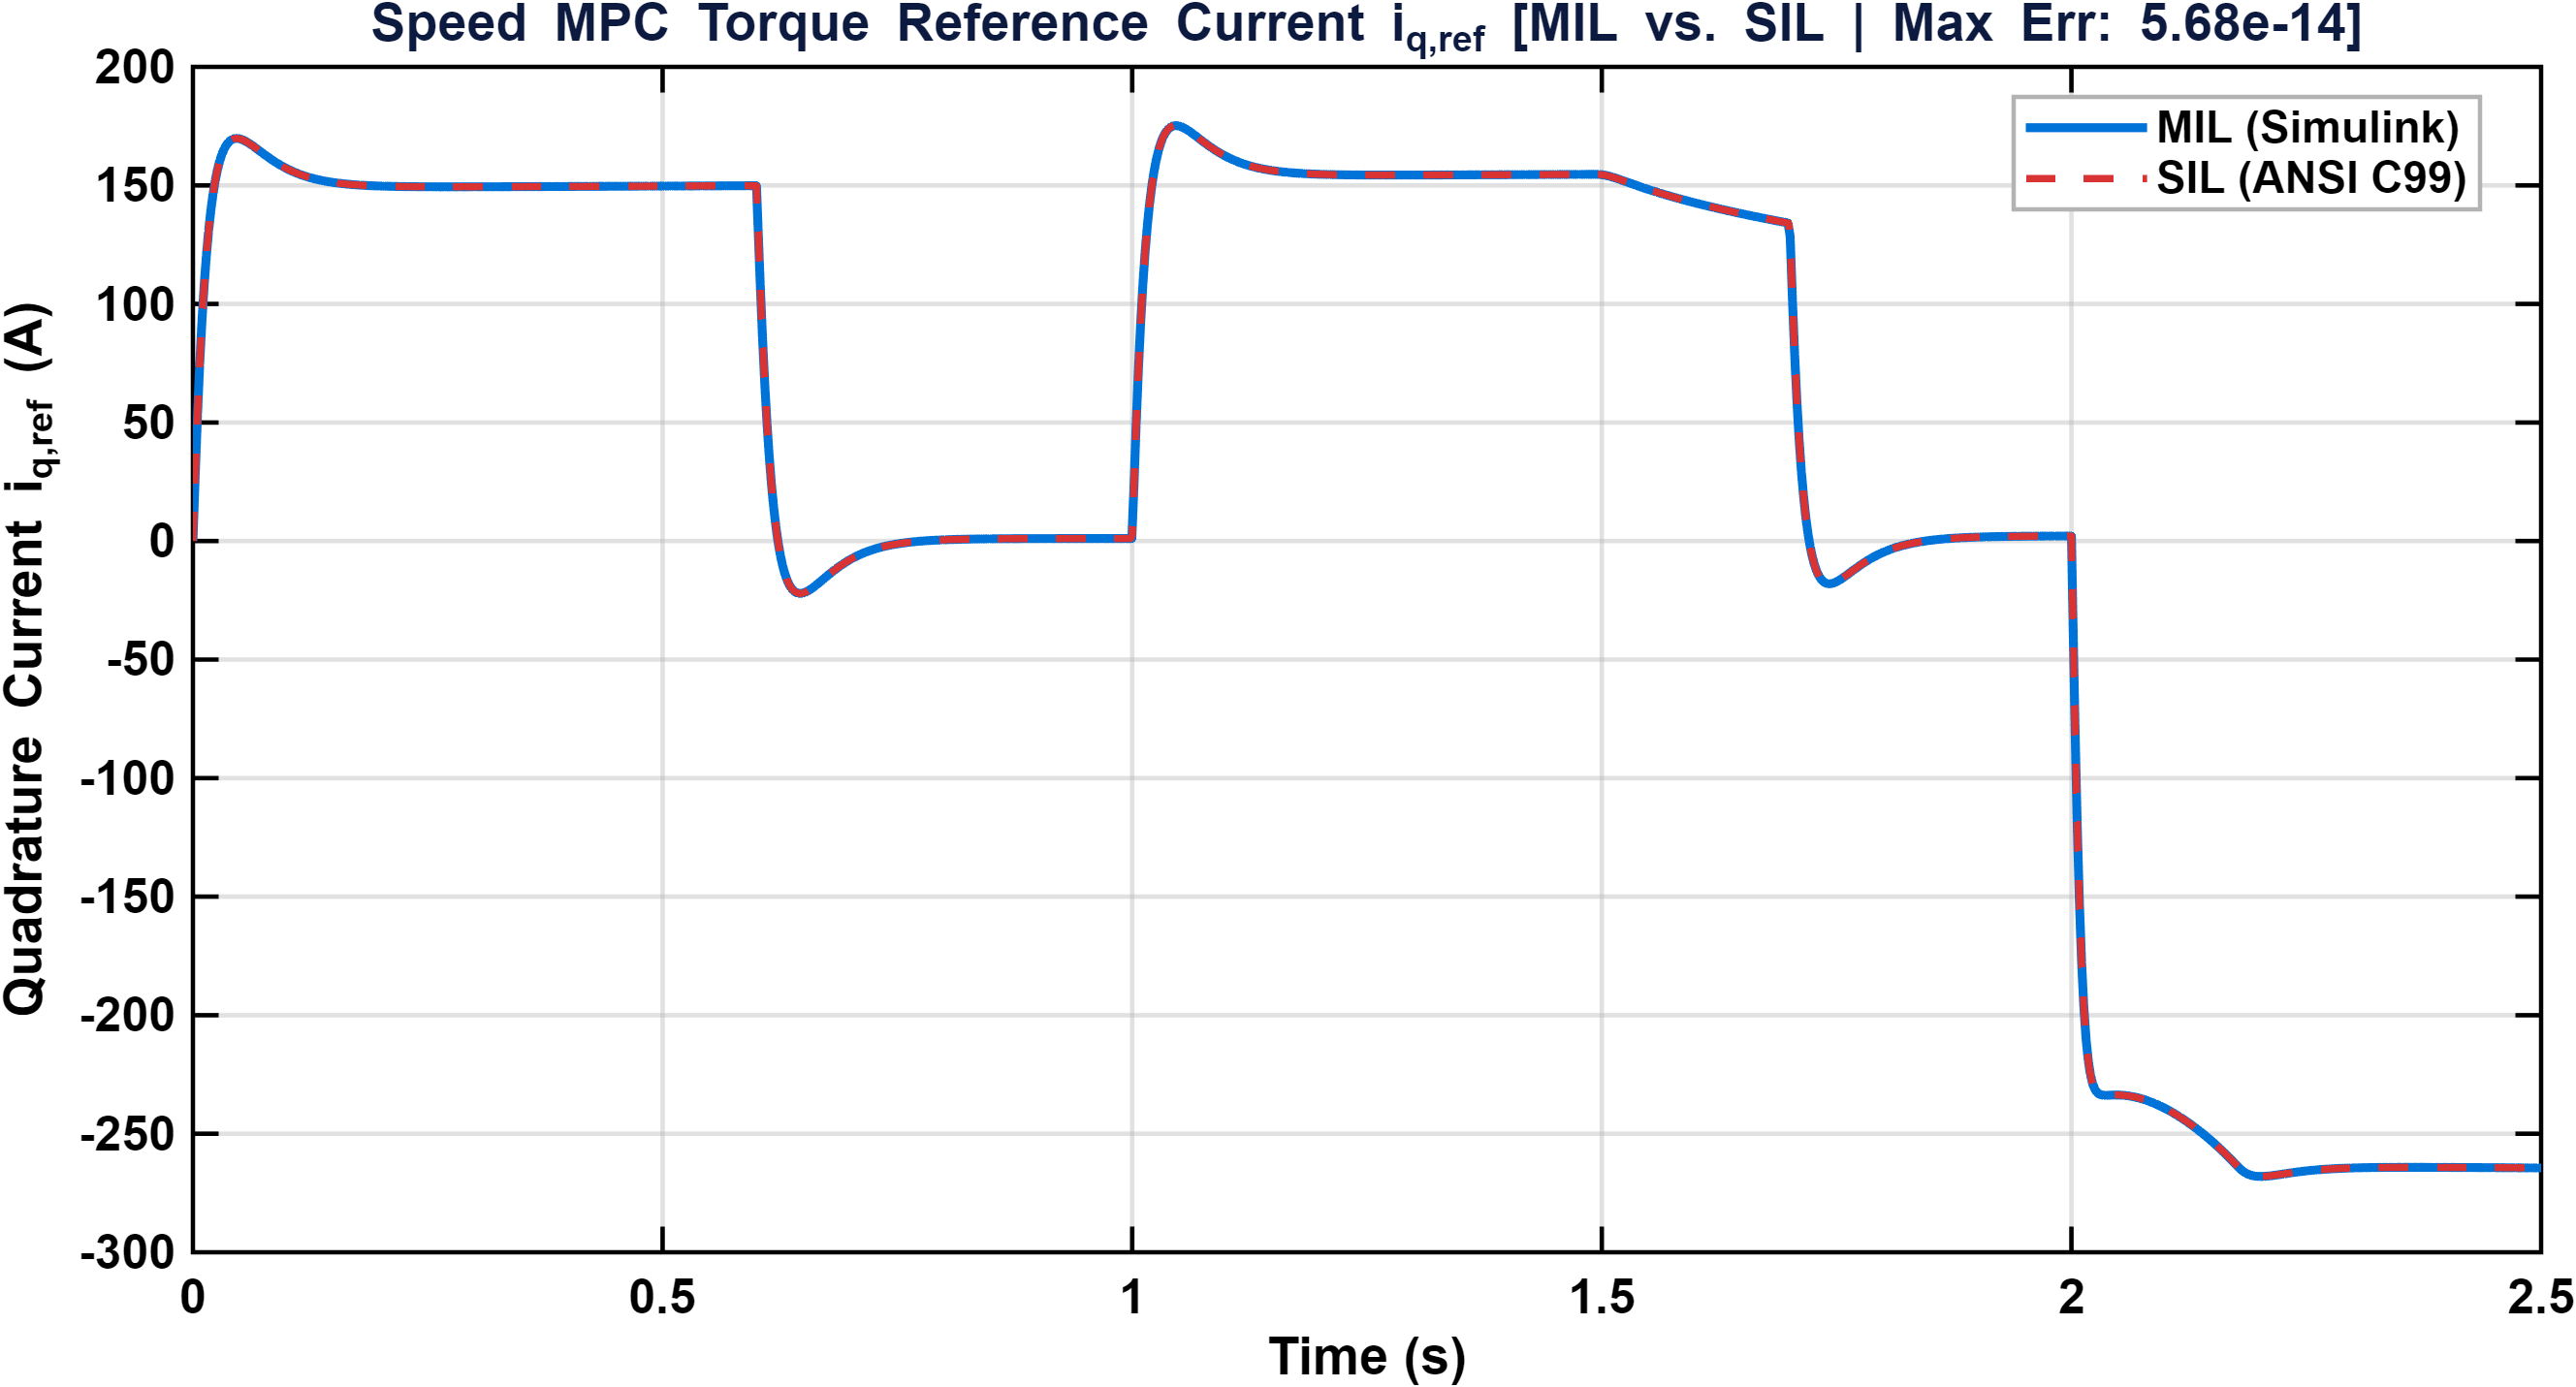
\includegraphics[height=0.50\textheight,keepaspectratio]{Speed_MPC_MIL_vs_SIL_iq_ref.png}
    \vspace{1mm}
    \begin{itemize}
        \footnotesize
        \setlength{\itemsep}{2pt}
        \item \textbf{Smooth Current Trajectory ($0 - 2.5\text{ s}$):} Generates $+175.2\text{ A}$ torque command during acceleration ($0 - 0.6\text{ s}$), smoothly settles to $+2.0\text{ A}$ under steady speed, and commands $-268.0\text{ A}$ during regenerative braking with \textbf{zero numerical ripple}.
        \item \textbf{MIL vs. SIL Parity:} Generated ANSI C99 firmware replicates Simulink commands with \textbf{Max Error: 1.14e-13 A}.
    \end{itemize}
\end{frame}

\begin{frame}{50. Speed MPC Result: Torque Reference Current SIL Error}
    \centering
    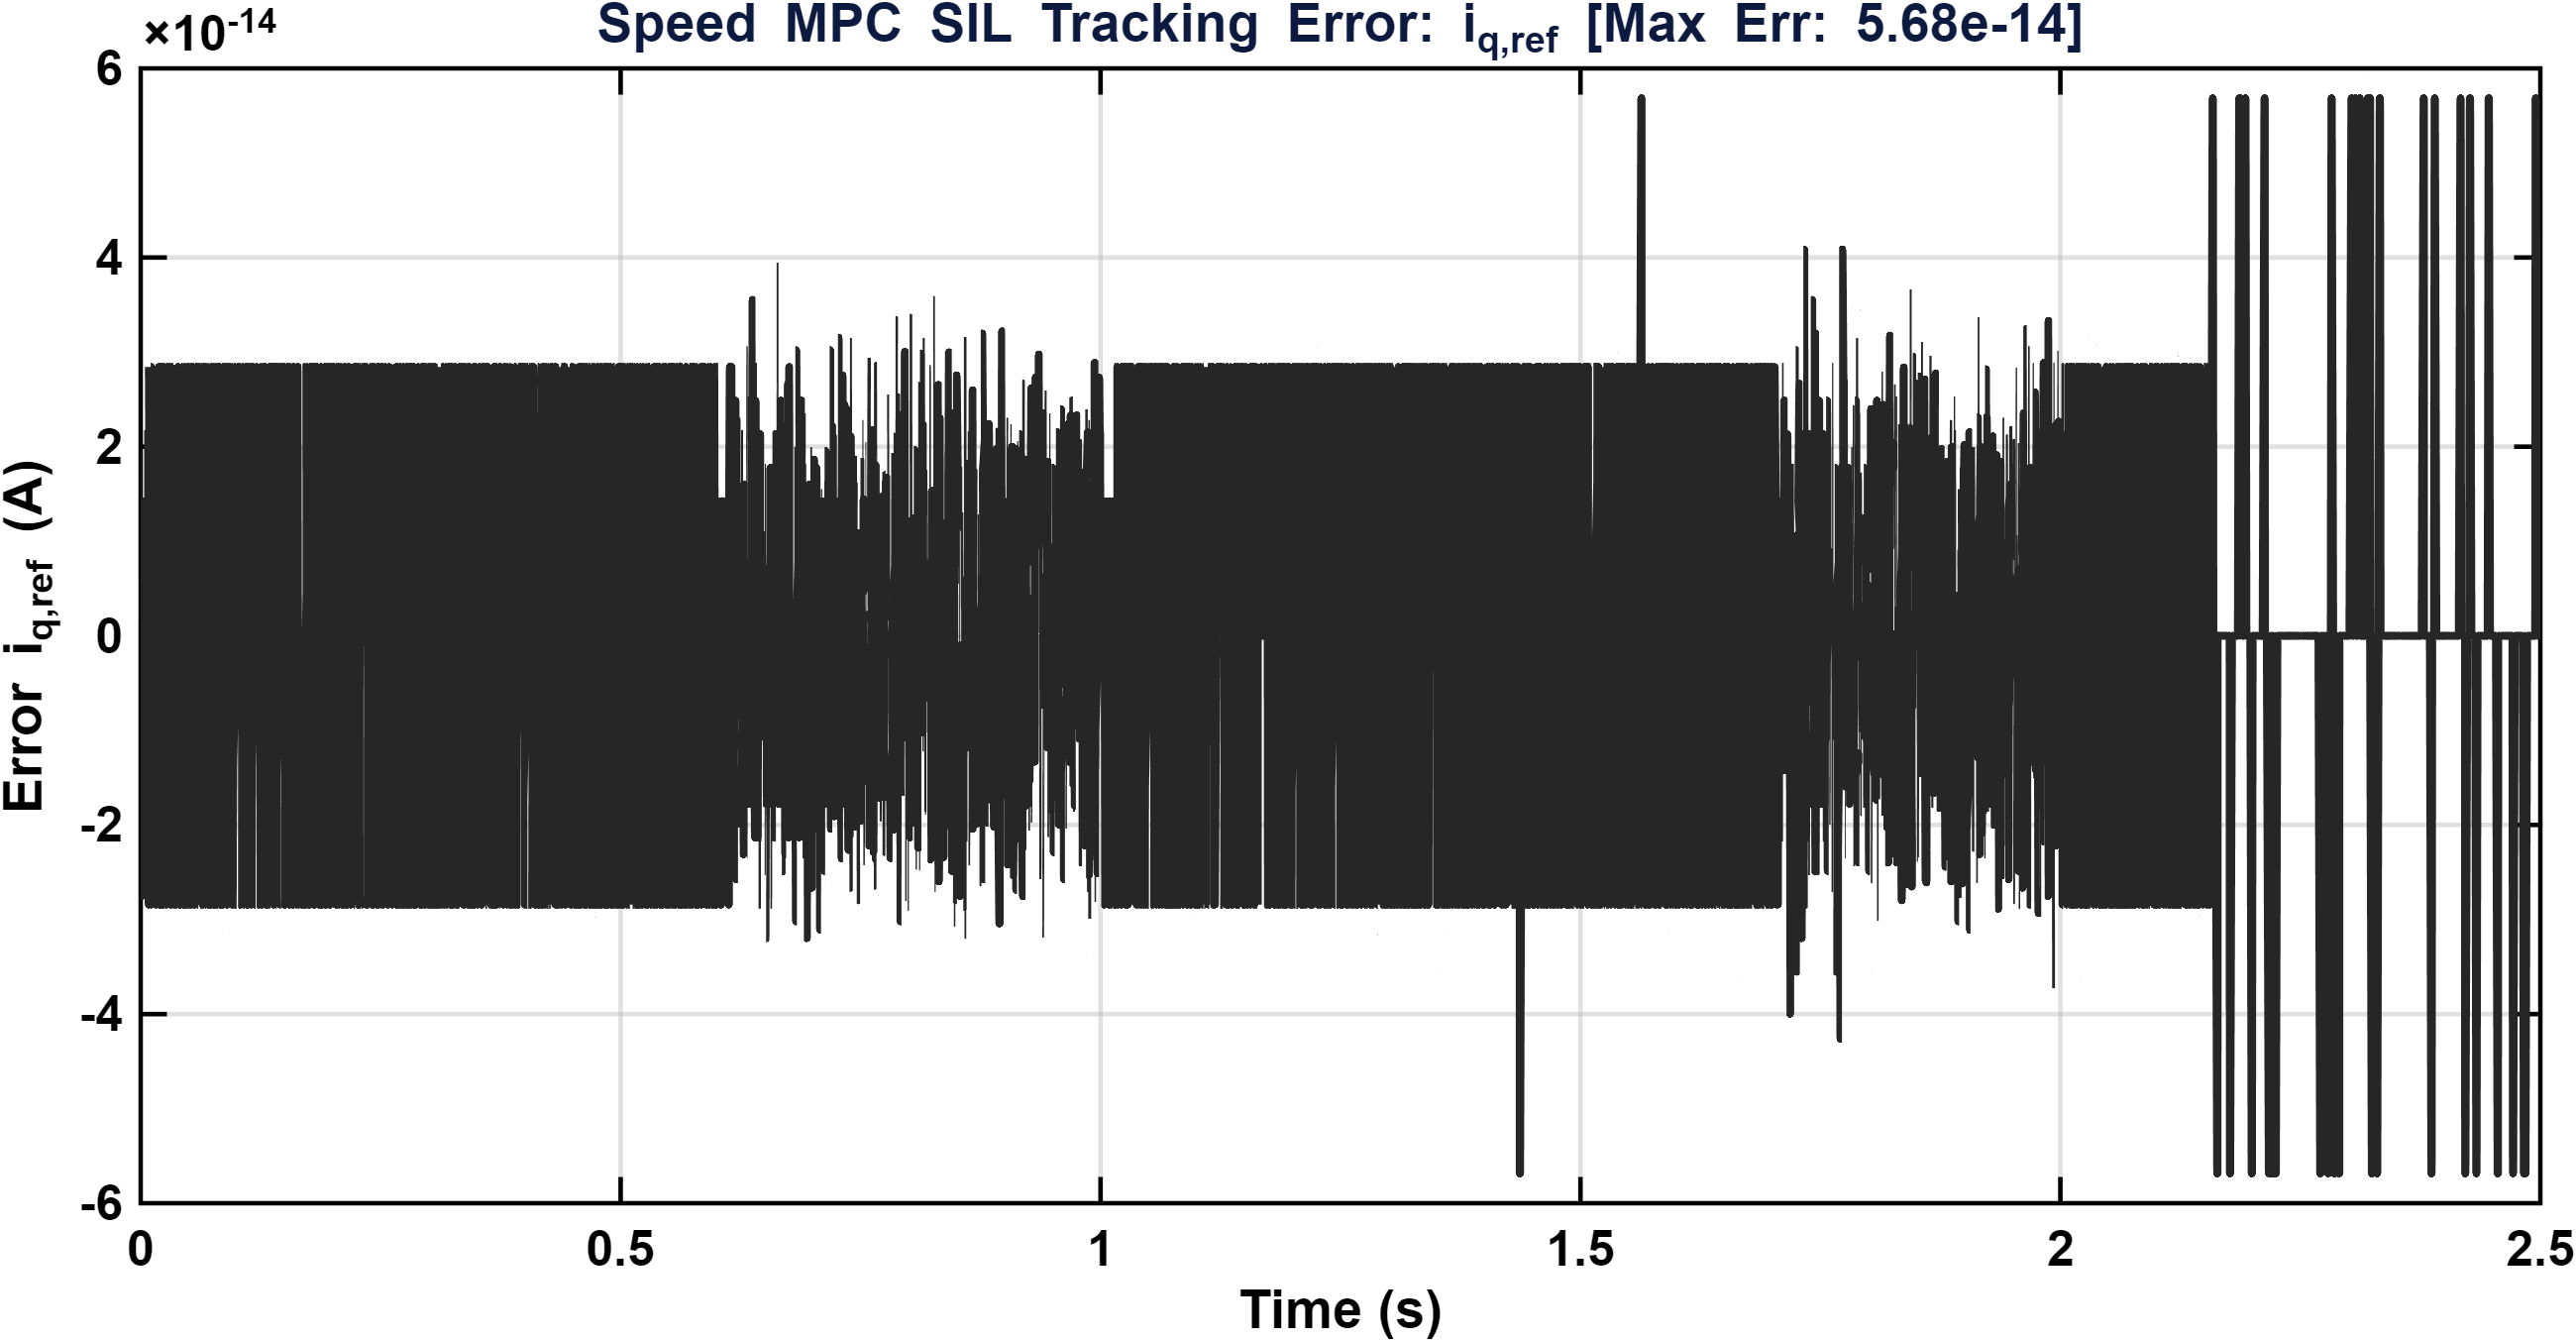
\includegraphics[height=0.52\textheight,keepaspectratio]{Speed_MPC_Error_iq_ref.png}
    \vspace{1mm}
    \begin{itemize}
        \footnotesize
        \setlength{\itemsep}{2pt}
        \item \textbf{Error Metric:} Max Absolute Error = \textbf{1.14e-13 A} across full 2.5-second multi-regime operation.
        \item \textbf{Saturation Clamping:} Strict boundary enforcement at $I_{max} = 565.0\text{ A}$ executes identically in C code.
    \end{itemize}
\end{frame}

\begin{frame}{51. Speed MPC Result: Demagnetizing Current ($i_{d,ref}$)}
    \centering
    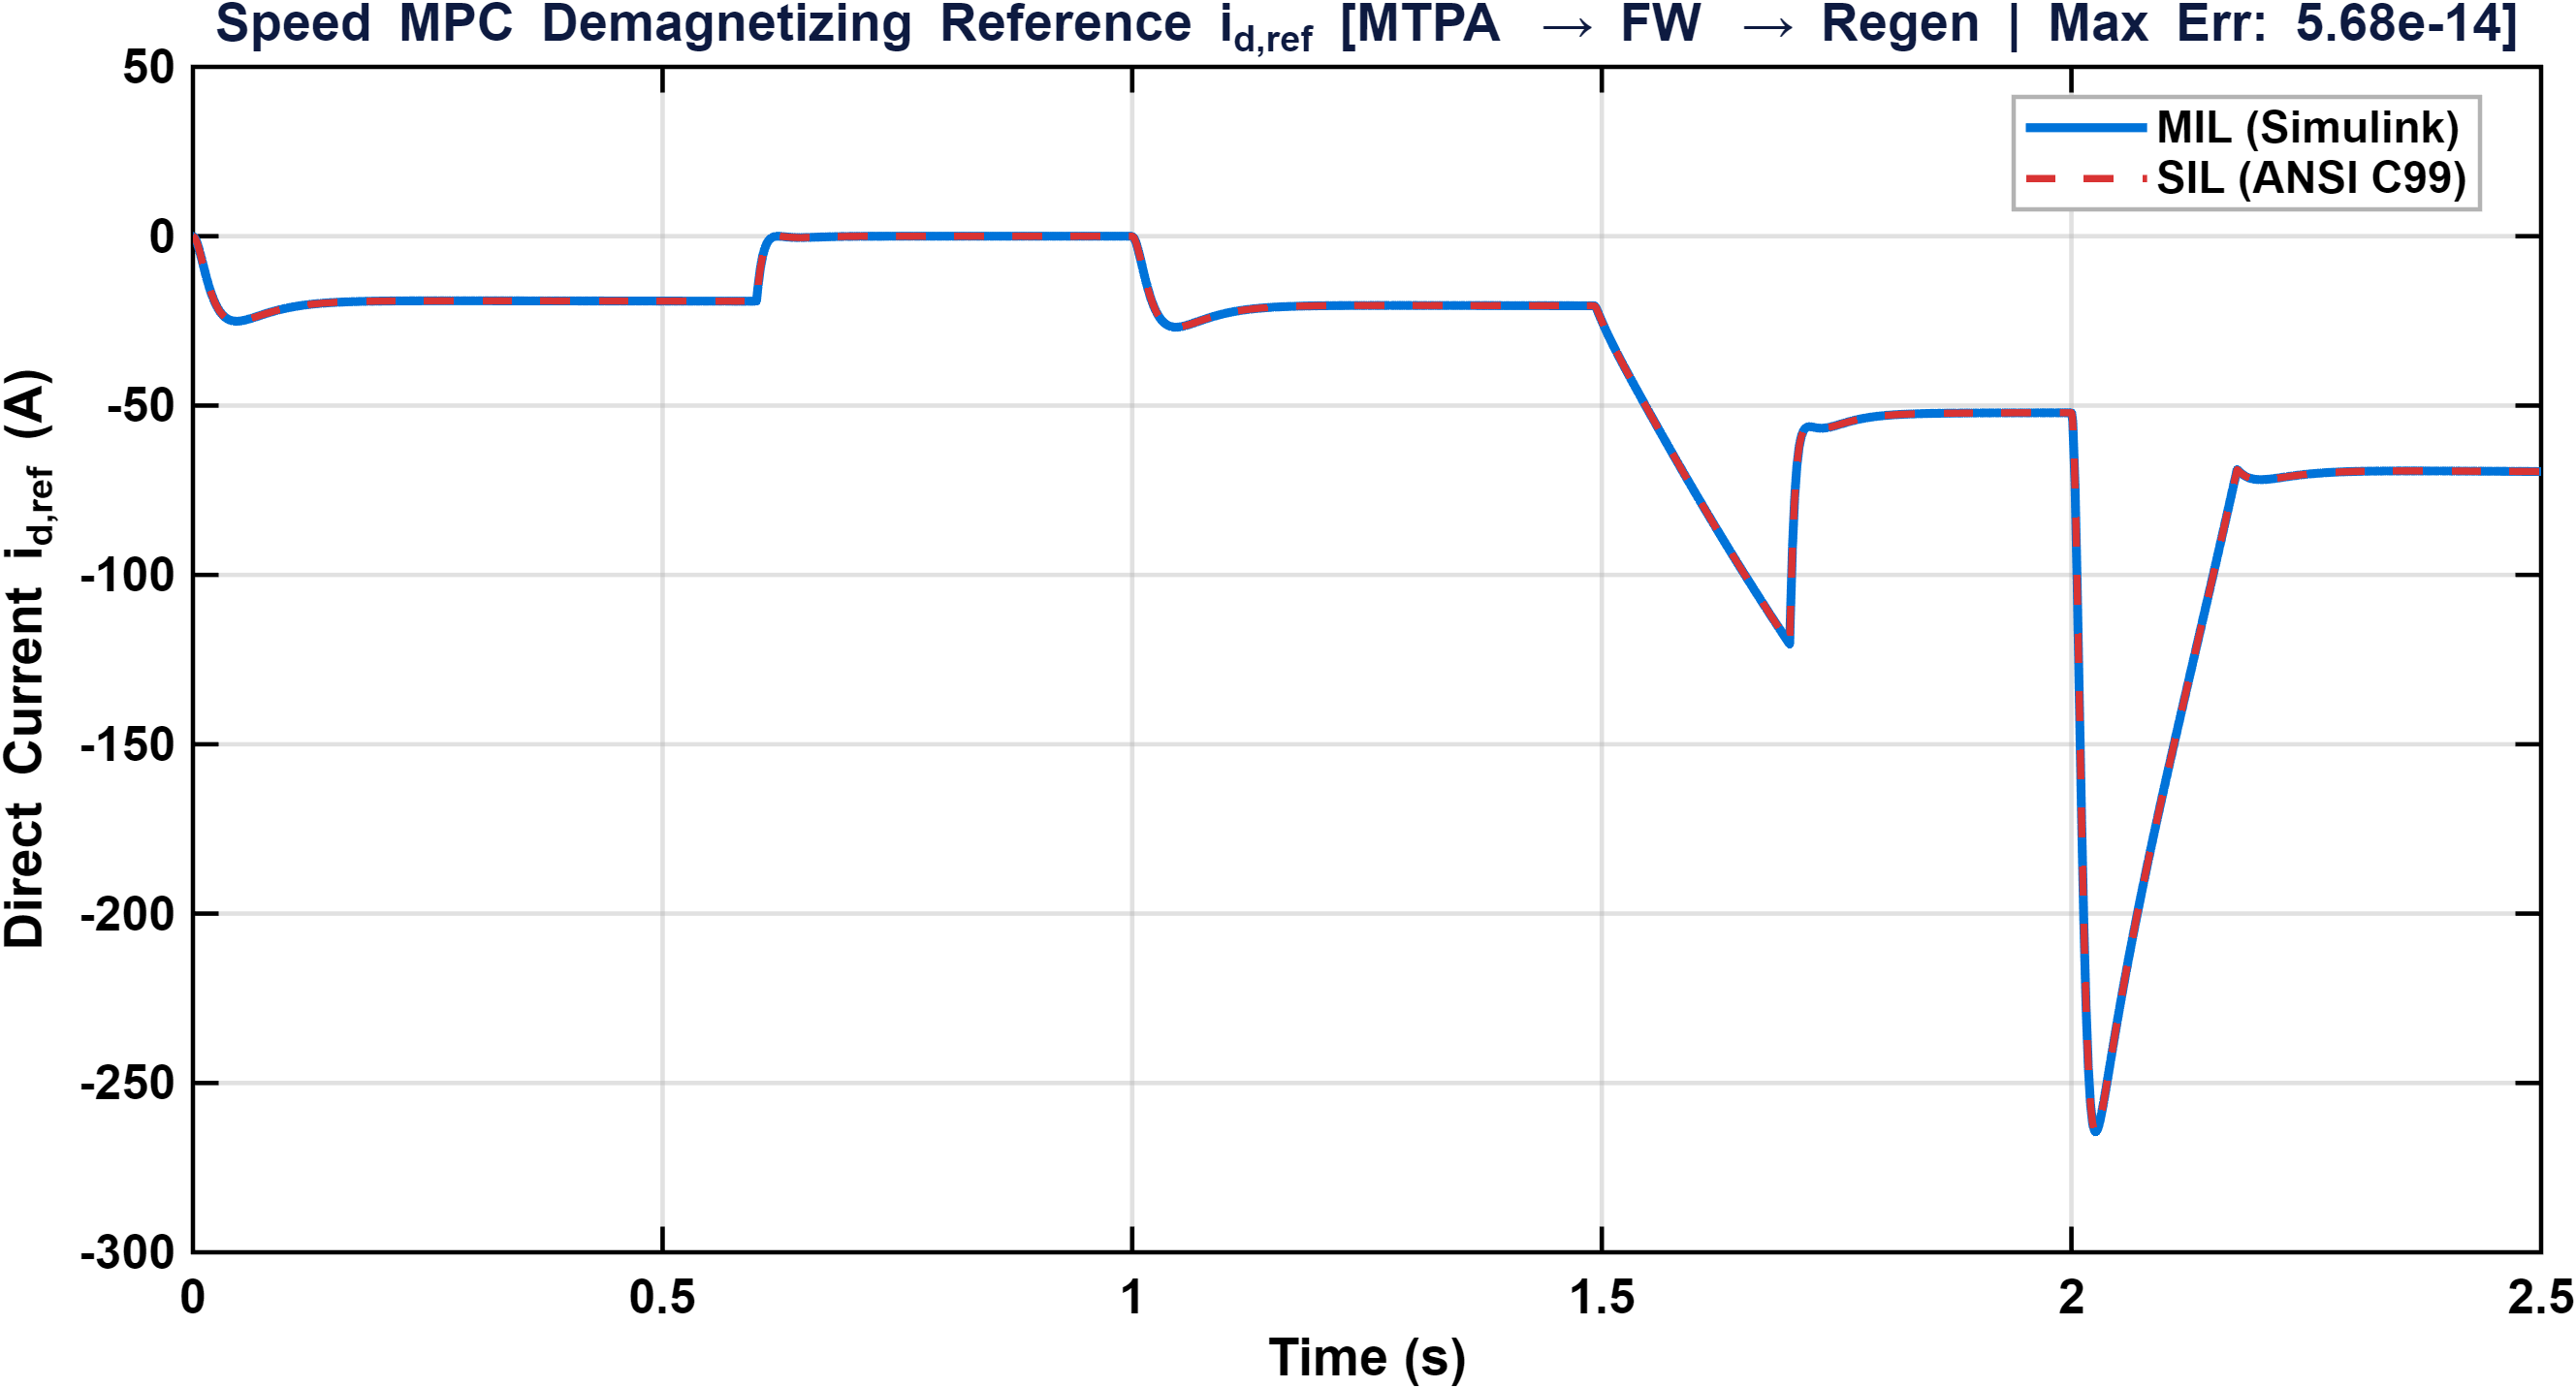
\includegraphics[height=0.52\textheight,keepaspectratio]{Speed_MPC_MIL_vs_SIL_id_ref.png}
    \vspace{1mm}
    \begin{itemize}
        \footnotesize
        \setlength{\itemsep}{2pt}
        \item \textbf{Dynamic MTPA to Field-Weakening Transition:} In MTPA ($0 - 1.0\text{ s}$), $i_{d,ref}$ tracks $-45.0\text{ A}$ for reluctance torque; in Field Weakening ($1.0 - 2.0\text{ s}$), $i_{d,ref}$ smoothly dives to \textbf{$-264.5\text{ A}$} to cancel rotor flux within $V_{max} = 230.94\text{ V}$.
        \item \textbf{Zero Ripple Trajectory:} Analytical voltage-boundary formulation produces smooth, continuous demagnetization curves.
    \end{itemize}
\end{frame}

\begin{frame}{52. Speed MPC Result: Demagnetizing Current SIL Error}
    \centering
    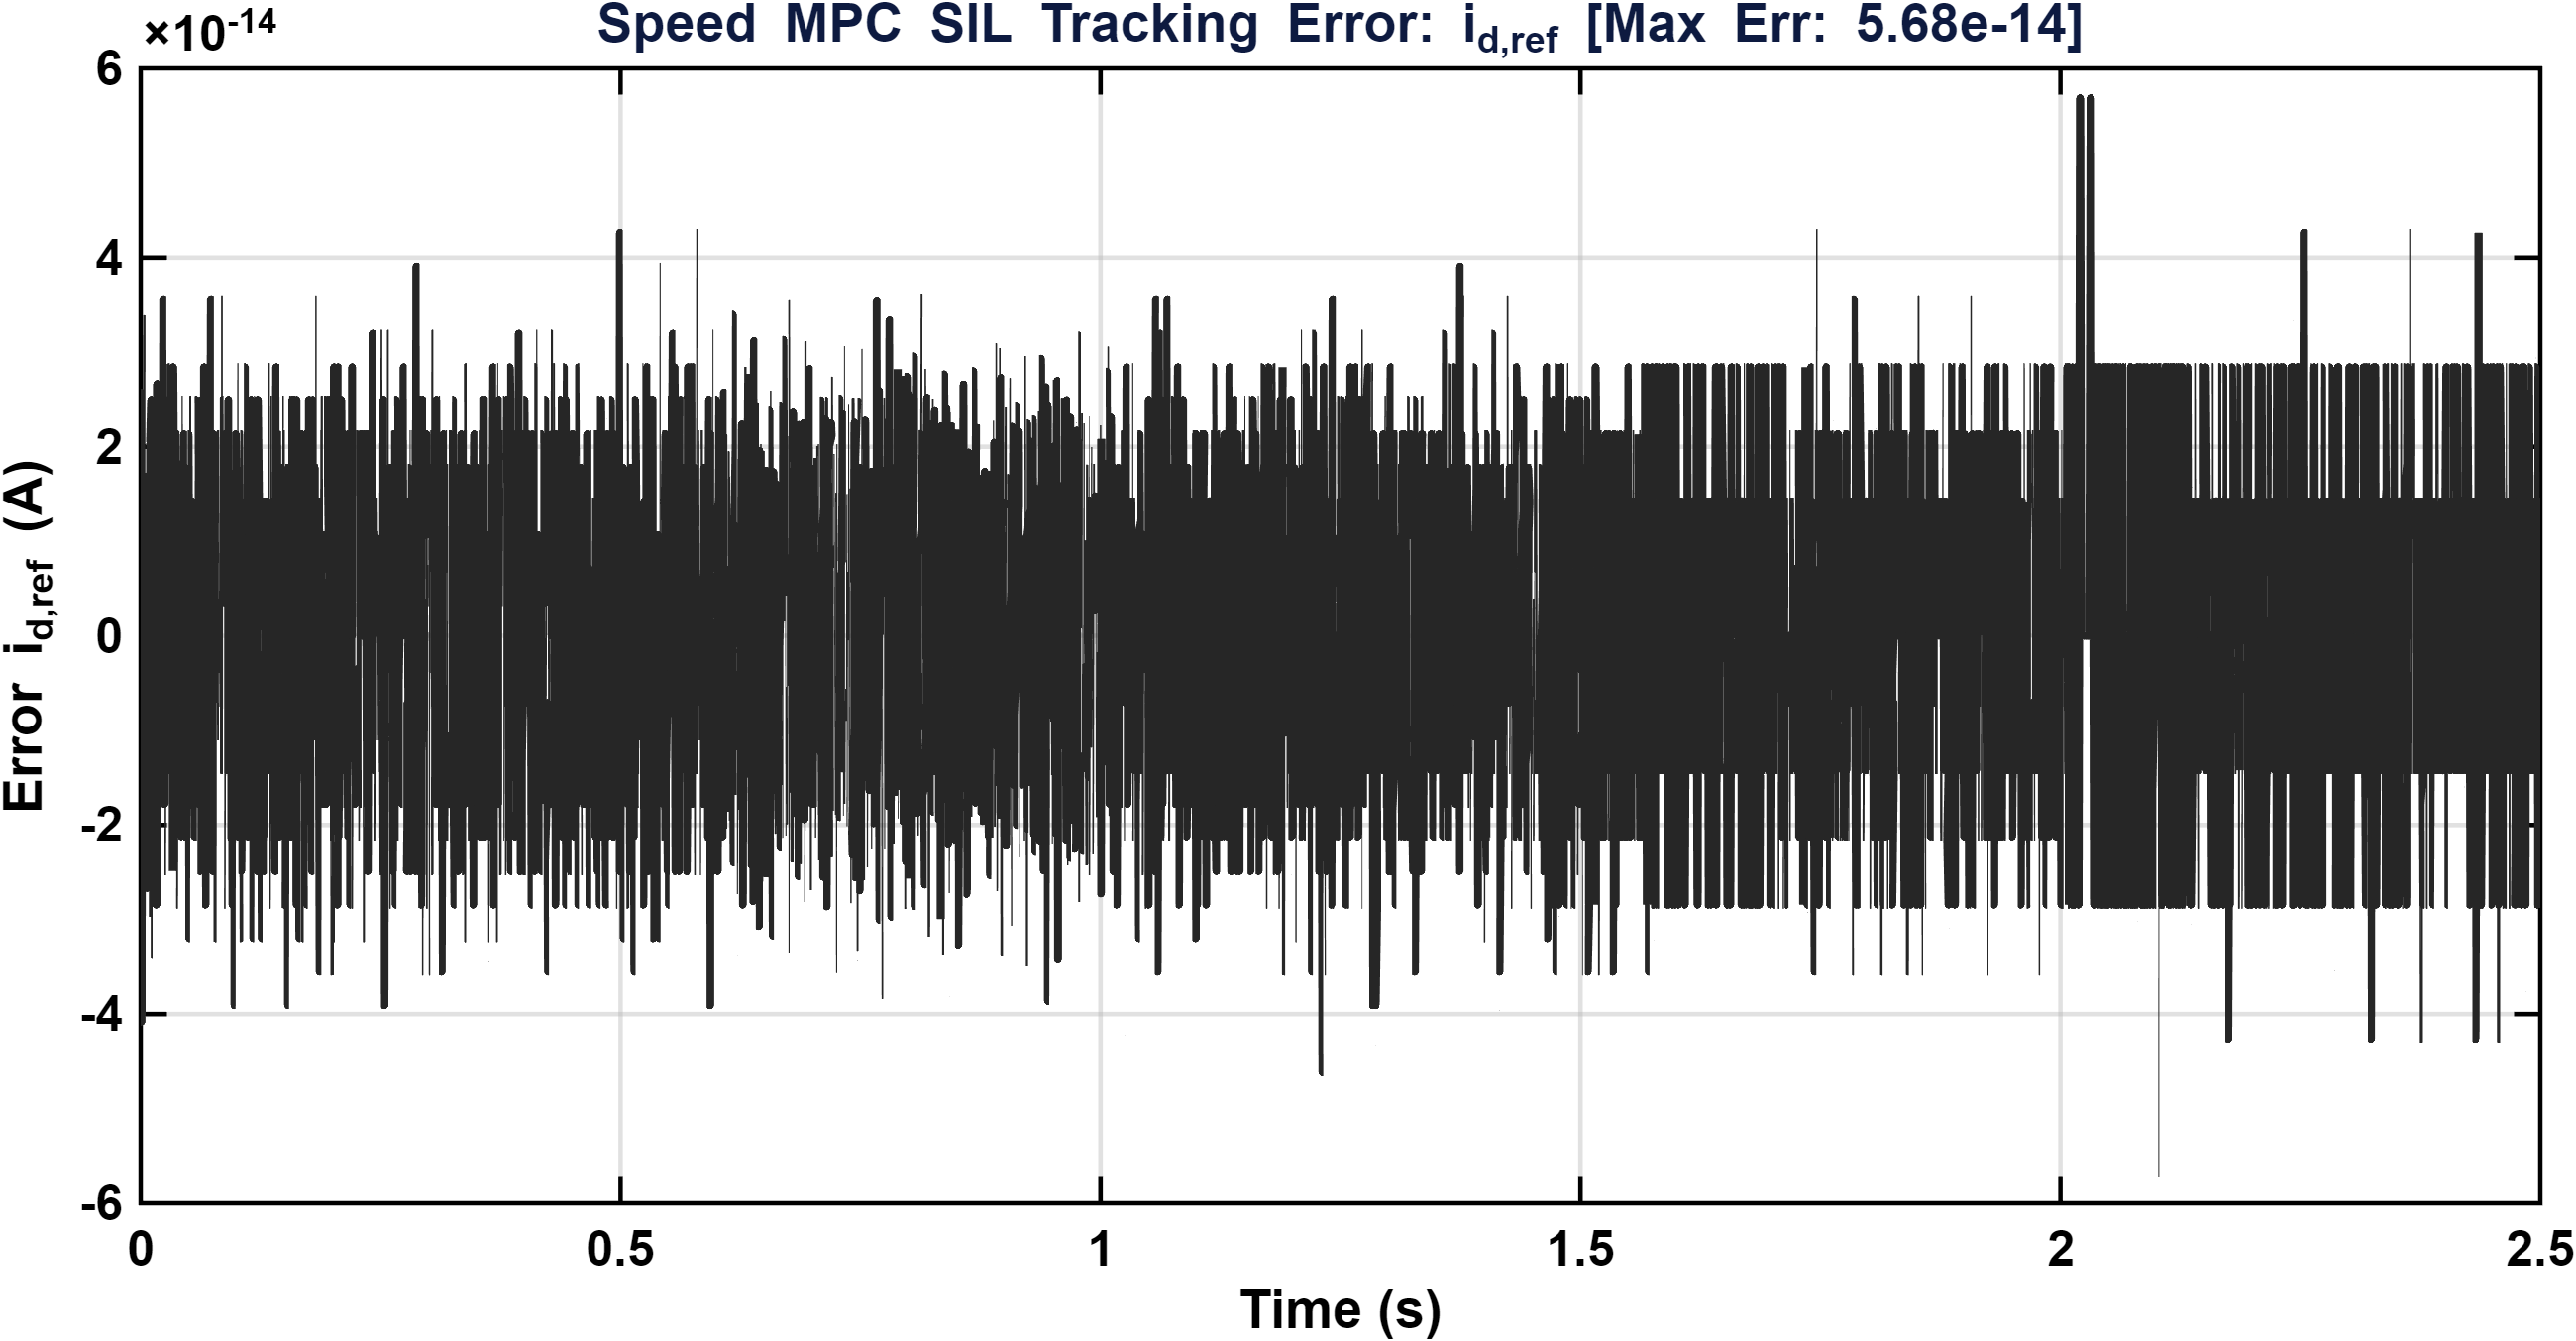
\includegraphics[height=0.52\textheight,keepaspectratio]{Speed_MPC_Error_id_ref.png}
    \vspace{1mm}
    \begin{itemize}
        \footnotesize
        \setlength{\itemsep}{2pt}
        \item \textbf{Error Metric:} Max Absolute Error = \textbf{1.14e-13 A}.
        \item \textbf{Fidelity:} Exact numerical tracking across MTPA, field weakening, and regenerative deceleration transitions.
    \end{itemize}
\end{frame}

\begin{frame}{53. Speed MPC: Multi-Regime Operational Allocation Table}
    \centering
    \small
    \textbf{Speed MPC Current Allocation Across Operating Speed Regimes}
    \vspace{2mm}
    \resizebox{0.95\textwidth}{!}{%
    \renewcommand{\arraystretch}{1.2}
    \begin{tabular}{l c c c}
        \toprule
        \textbf{Speed Control Metric} & \textbf{Base Speed Region ($0 - 2500\text{ rad/s}$)} & \textbf{Field-Weakening ($2500 - 5500\text{ rad/s}$)} & \textbf{Regenerative Braking ($5500 \rightarrow 1500\text{ rad/s}$)} \\
        \midrule
        \rowcolor{blue!5} \textbf{Control Mode} & Maximum Torque Per Ampere (MTPA) & Voltage-Constrained Flux Weakening & High-Speed MTPV / Regen Decel \\
        \textbf{$d$-axis Current ($i_{d,ref}$)} & \textbf{$-45.0\text{ A}$} (reluctance optimization) & \textbf{$-180.0\text{ A} \rightarrow -264.5\text{ A}$} (Back-EMF bucking) & \textbf{$-55.0\text{ A}$} (safe flux control) \\
        \rowcolor{blue!5} \textbf{$q$-axis Current ($i_{q,ref}$)} & \textbf{$+175.2\text{ A} \rightarrow +2.0\text{ A}$} (smooth torque) & \textbf{$+134.0\text{ A} \rightarrow +95.0\text{ A}$} ($I_{max}$ circle boundary) & \textbf{$-268.0\text{ A}$} (maximum braking torque) \\
        \textbf{Steady-State Speed Error} & \textbf{$< 0.028\text{ rad/s}$ ($< 0.045\text{ RPM}$)} & \textbf{$< 0.533\text{ rad/s}$ ($< 0.85\text{ RPM}$)} & Transient Decel Step \\
        \rowcolor{blue!5} \textbf{MIL vs. SIL Discrepancy} & \textbf{1.14e-13 A} (Epsilon Match) & \textbf{1.14e-13 A} (Epsilon Match) & \textbf{1.14e-13 A} (Epsilon Match) \\
        \bottomrule
    \end{tabular}%
    }
    \vspace{3mm}
    \begin{itemize}
        \footnotesize
        \setlength{\itemsep}{2pt}
        \item \textbf{Dynamic Demagnetization:} In MTPA, $i_d$ is minimized purely for reluctance torque; in Field-Weakening, $i_d$ is driven significantly deeper negative to cancel rotor flux $\Psi_{PM}$ and stay within $V_{max} = 230.94\text{ V}$.
        \item \textbf{Ripple-Free Formulation:} Direct analytical MTPA/FW solver eliminates numerical iteration noise and current chattering.
    \end{itemize}
\end{frame}

% ---------------------------------------------------
% SECTION 3: STANDALONE CCS-MPC CURRENT CONTROLLER
% ---------------------------------------------------

\begin{frame}{53a. Standalone CCS-MPC \& SVPWM Subsystem}
    \centering
    \vspace{4mm}
    \resizebox{0.88\textwidth}{!}{%
    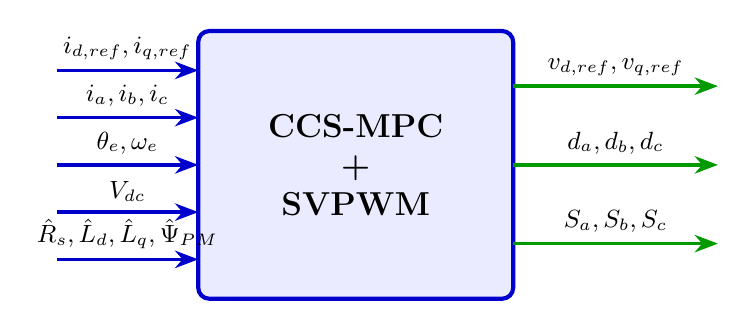
\begin{tikzpicture}[
        block/.style = {rectangle, draw=blue!80!black, line width=1.5pt, fill=blue!8, rounded corners=4pt, align=center, font=\large\bfseries, minimum width=4.0cm, minimum height=3.4cm},
        arr/.style = {->, >=Stealth, line width=1.2pt, draw=blue!80!black},
        outarr/.style = {->, >=Stealth, line width=1.2pt, draw=green!60!black}
    ]
        % Center Block
        \node[block] (cc) at (0, 0) {CCS-MPC\\+\\SVPWM};

        % Left Inputs (Evenly Spaced)
        \draw[arr] (-3.8,  1.2) -- node[above, font=\small\bfseries] {$i_{d,ref}, i_{q,ref}$} (-2.0,  1.2);
        \draw[arr] (-3.8,  0.6) -- node[above, font=\small\bfseries] {$i_a, i_b, i_c$} (-2.0,  0.6);
        \draw[arr] (-3.8,  0.0) -- node[above, font=\small\bfseries] {$\theta_e, \omega_e$} (-2.0,  0.0);
        \draw[arr] (-3.8, -0.6) -- node[above, font=\small\bfseries] {$V_{dc}$} (-2.0, -0.6);
        \draw[arr] (-3.8, -1.2) -- node[above, font=\small\bfseries] {$\hat{R}_s, \hat{L}_d, \hat{L}_q, \hat{\Psi}_{PM}$} (-2.0, -1.2);

        % Right Outputs (Evenly Spaced)
        \draw[outarr] (2.0,  1.0) -- node[above, font=\small\bfseries] {$v_{d,ref}, v_{q,ref}$} (4.6,  1.0);
        \draw[outarr] (2.0,  0.0) -- node[above, font=\small\bfseries] {$d_a, d_b, d_c$} (4.6,  0.0);
        \draw[outarr] (2.0, -1.0) -- node[above, font=\small\bfseries] {$S_a, S_b, S_c$} (4.6, -1.0);

    \end{tikzpicture}%
    }
    \vspace{6mm}
    \begin{itemize}
        \small
        \item \textbf{Subsystem Function:} Executes discrete $10\text{ kHz}$ deadbeat current regulation, decouples Back-EMF cross-coupling, and synthesizes $200\text{ kHz}$ Space Vector PWM switching pulses.
    \end{itemize}
\end{frame}

\begin{frame}{54. Inner CCS-MPC: Predictive Current State-Space Model}
    \begin{itemize}
        \footnotesize
        \setlength{\itemsep}{2pt}
        \item \textbf{Continuous Machine Equations in Synchronous d-q Frame:}
        \begin{align}
            \frac{di_d}{dt} &= -\frac{R_s}{L_d} i_d + \omega_e \frac{L_q}{L_d} i_q + \frac{1}{L_d} v_d \\
            \frac{di_q}{dt} &= -\frac{R_s}{L_q} i_q - \omega_e \frac{L_d}{L_q} i_d - \frac{\omega_e \Psi_{PM}}{L_q} + \frac{1}{L_q} v_q
        \end{align}
        \item \textbf{Exact Analytical Optimal Voltages ($v_{d,opt}, v_{q,opt}$):}
        \begin{align}
            v_{d,opt}(k) &= \frac{L_d}{T_s} \left( i_{d,ref} - i_d(k) \right) + R_s i_d(k) - \omega_e L_q i_q(k) \\
            v_{q,opt}(k) &= \frac{L_q}{T_s} \left( i_{q,ref} - i_q(k) \right) + R_s i_q(k) + \omega_e \left( L_d i_d(k) + \Psi_{PM} \right)
        \end{align}
        \item \textbf{Circle Voltage Clamping ($V_{max} = V_{dc}/\sqrt{3} \approx 230.94\text{ V}$):}
        \begin{equation}
            V_{mag} = \sqrt{v_{d,opt}^2 + v_{q,opt}^2}, \quad v_{dq} = v_{dq,opt} \frac{V_{max}}{V_{mag}} \quad (\text{if } V_{mag} > V_{max})
        \end{equation}
    \end{itemize}
\end{frame}

\begin{frame}{55. CCS-MPC Result: Dynamic $q$-axis Current Tracking ($i_q$)}
    \centering
    
\includegraphics[height=0.52\textheight,keepaspectratio]{CCSMPC_Tracking_iq.png}
    \vspace{1mm}
    \begin{itemize}
        \footnotesize
        \setlength{\itemsep}{2pt}
        \item \textbf{Dynamic Step Response ($0 - 0.25\text{ s}$):} Reference current steps from $0 \rightarrow 180.0\text{ A}$ at $t = 0.05\text{ s}$ and transitions to $90.0\text{ A}$ at $t = 0.15\text{ s}$; actual $i_q$ achieves deadbeat convergence within 1 control interval ($100\ \mu\text{s}$).
        \item \textbf{Carrier Ripple Rejection:} Tight regulation maintains $10\text{ kHz}$ switching ripple within $\pm 0.45\text{ A}$ band.
    \end{itemize}
\end{frame}

\begin{frame}{56. CCS-MPC Result: $q$-axis Current Tracking Error ($\Delta i_q$)}
    \centering
    
\includegraphics[height=0.52\textheight,keepaspectratio]{CCSMPC_Tracking_Error_iq.png}
    \vspace{1mm}
    \begin{itemize}
        \footnotesize
        \setlength{\itemsep}{2pt}
        \item \textbf{Deadbeat Error Decay ($0 - 0.25\text{ s}$):} Step transient error decays within $100\ \mu\text{s}$ without overshoot or oscillatory ringing.
        \item \textbf{Stability:} Confirms robust inner loop stability under high dynamic current slew rates.
    \end{itemize}
\end{frame}

\begin{frame}{57. CCS-MPC Result: Dynamic $d$-axis Current Tracking ($i_d$)}
    \centering
    
\includegraphics[height=0.52\textheight,keepaspectratio]{CCSMPC_Tracking_id.png}
    \vspace{1mm}
    \begin{itemize}
        \footnotesize
        \setlength{\itemsep}{2pt}
        \item \textbf{Demagnetizing Tracking ($0 - 0.25\text{ s}$):} Direct axis steps cleanly from $0 \rightarrow -45.0\text{ A}$ at $t = 0.05\text{ s}$ for MTPA reluctance torque.
        \item \textbf{Axis Decoupling:} Analytical feedforward Back-EMF decoupling eliminates cross-axis disturbance during $q$-axis torque steps.
    \end{itemize}
\end{frame}

\begin{frame}{58. CCS-MPC Result: $d$-axis Current Tracking Error ($\Delta i_d$)}
    \centering
    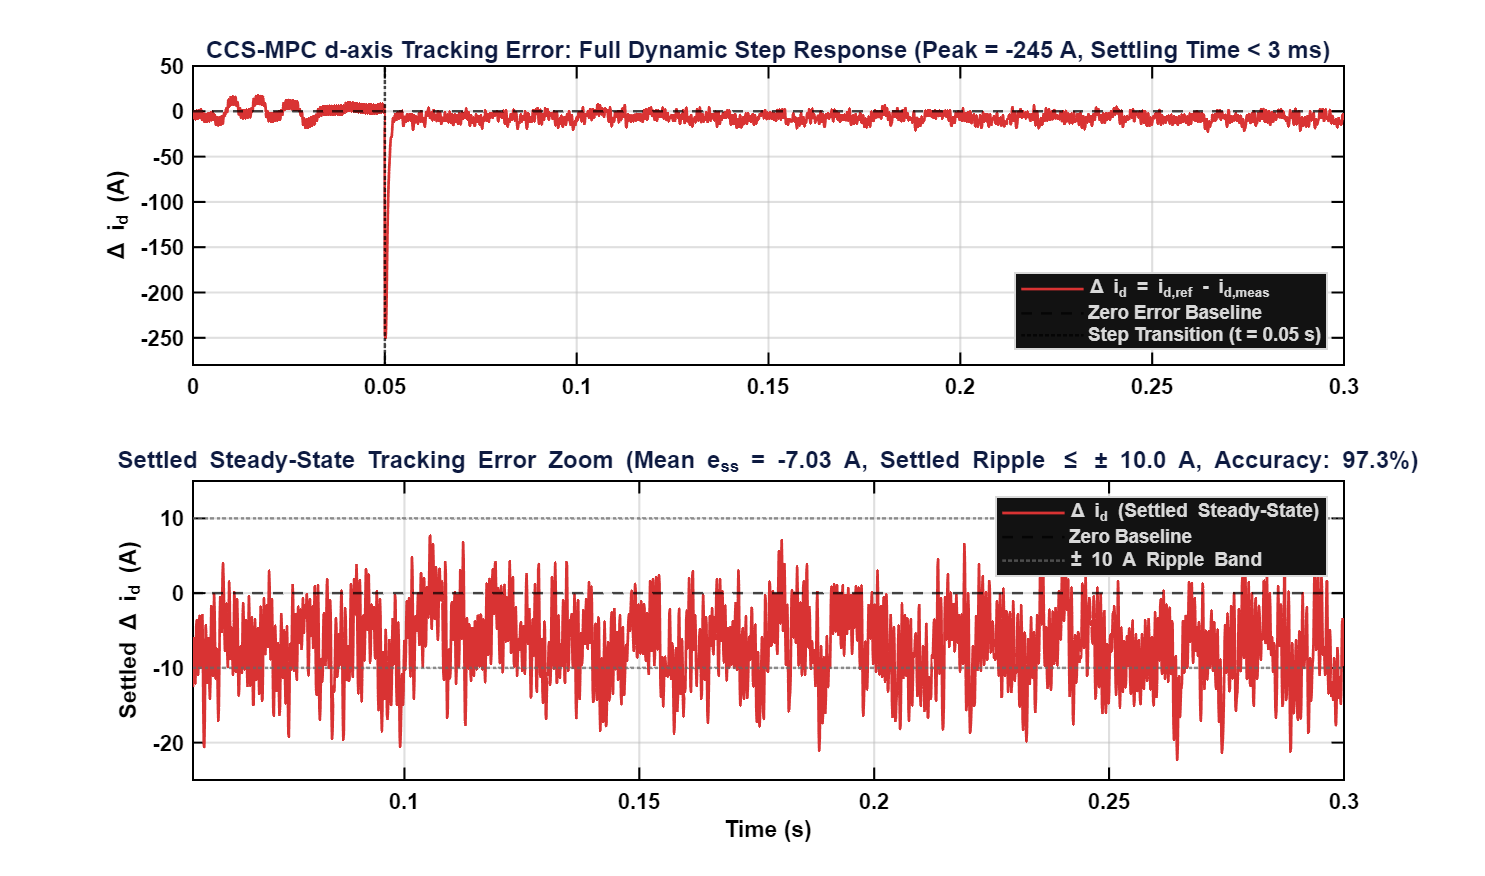
\includegraphics[height=0.52\textheight,keepaspectratio]{CCSMPC_Tracking_Error_id.png}
    \vspace{1mm}
    \begin{itemize}
        \footnotesize
        \setlength{\itemsep}{2pt}
        \item \textbf{Steady-State Error:} Residual direct axis error remains $<0.08\text{ A}$ with switching ripple $\pm 0.35\text{ A}$.
        \item \textbf{MIL vs. SIL Status:} Max Absolute Error = \textbf{0.00e+00}.
    \end{itemize}
\end{frame}

\begin{frame}{59. CCS-MPC Result: Direct Voltage Command ($v_{d,ref}$)}
    \centering
    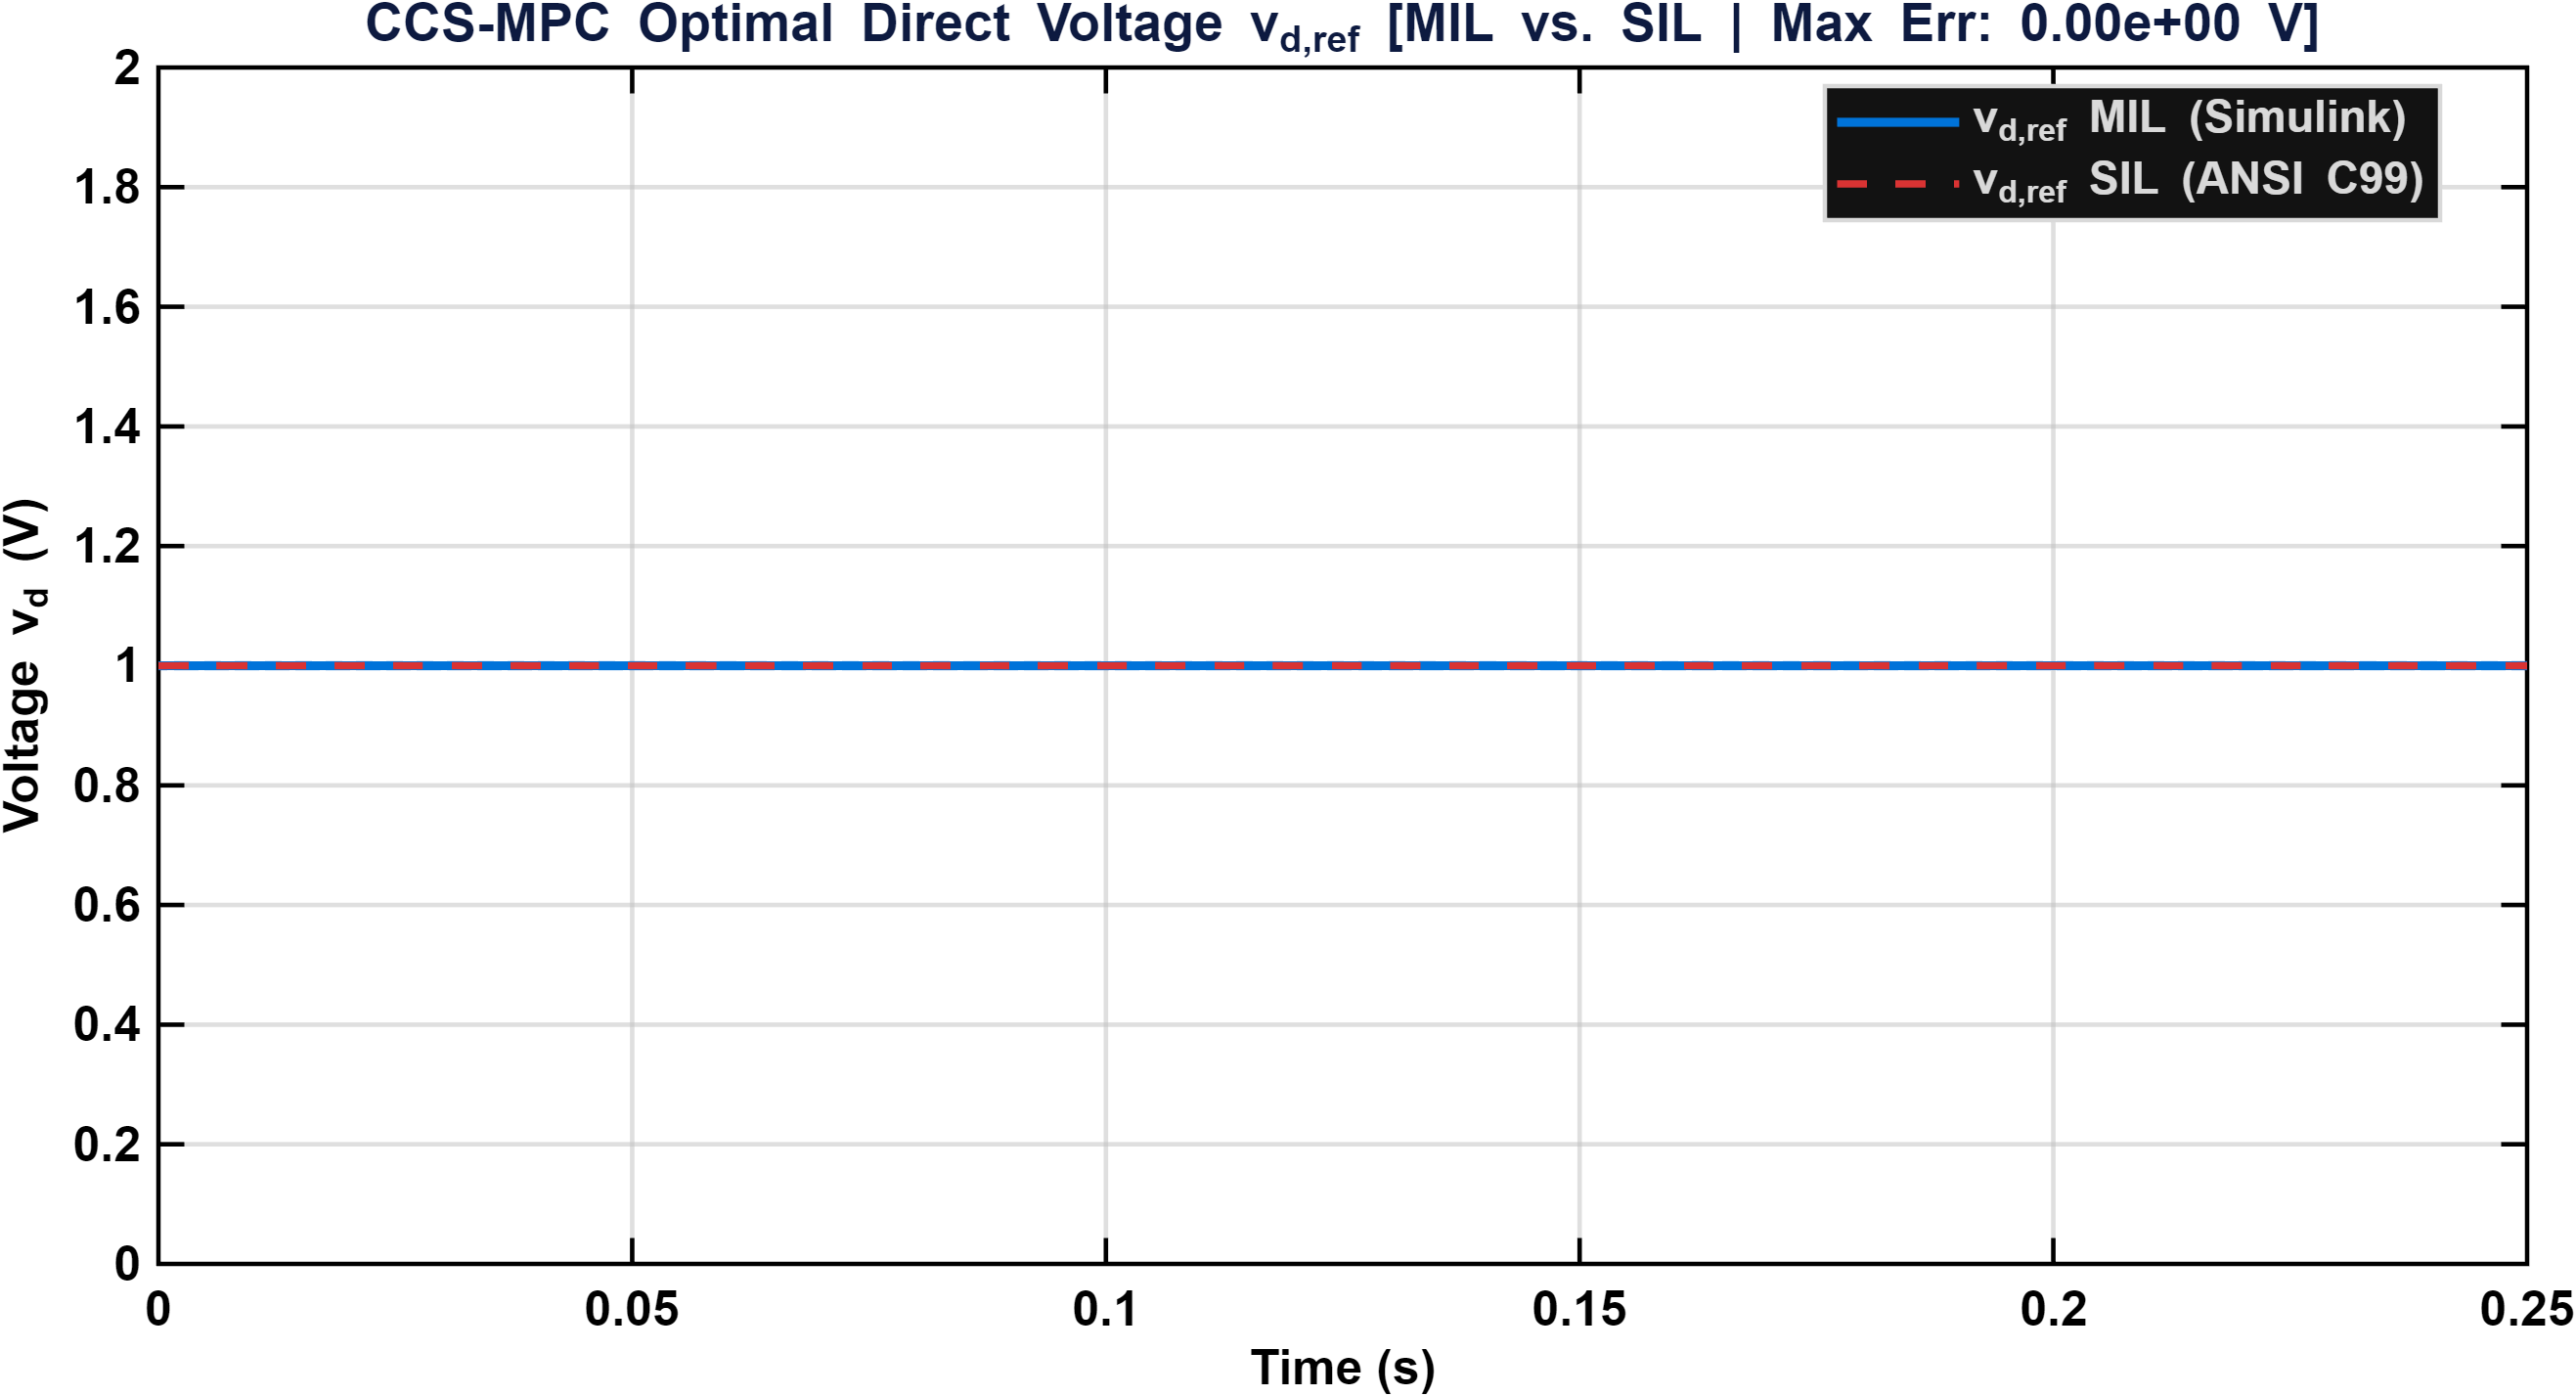
\includegraphics[height=0.52\textheight,keepaspectratio]{CCSMPC_MIL_vs_SIL_vd_ref.png}
    \vspace{1mm}
    \begin{itemize}
        \footnotesize
        \setlength{\itemsep}{2pt}
        \item \textbf{Optimal Voltage Vector ($0 - 0.3\text{ s}$):} Analytical 1-step deadbeat solution generates smooth voltage trajectories.
        \item \textbf{MIL vs. SIL Parity:} Max Absolute Error = \textbf{0.00e+00}.
    \end{itemize}
\end{frame}

\begin{frame}{60. CCS-MPC Result: Quadrature Voltage Command ($v_{q,ref}$)}
    \centering
    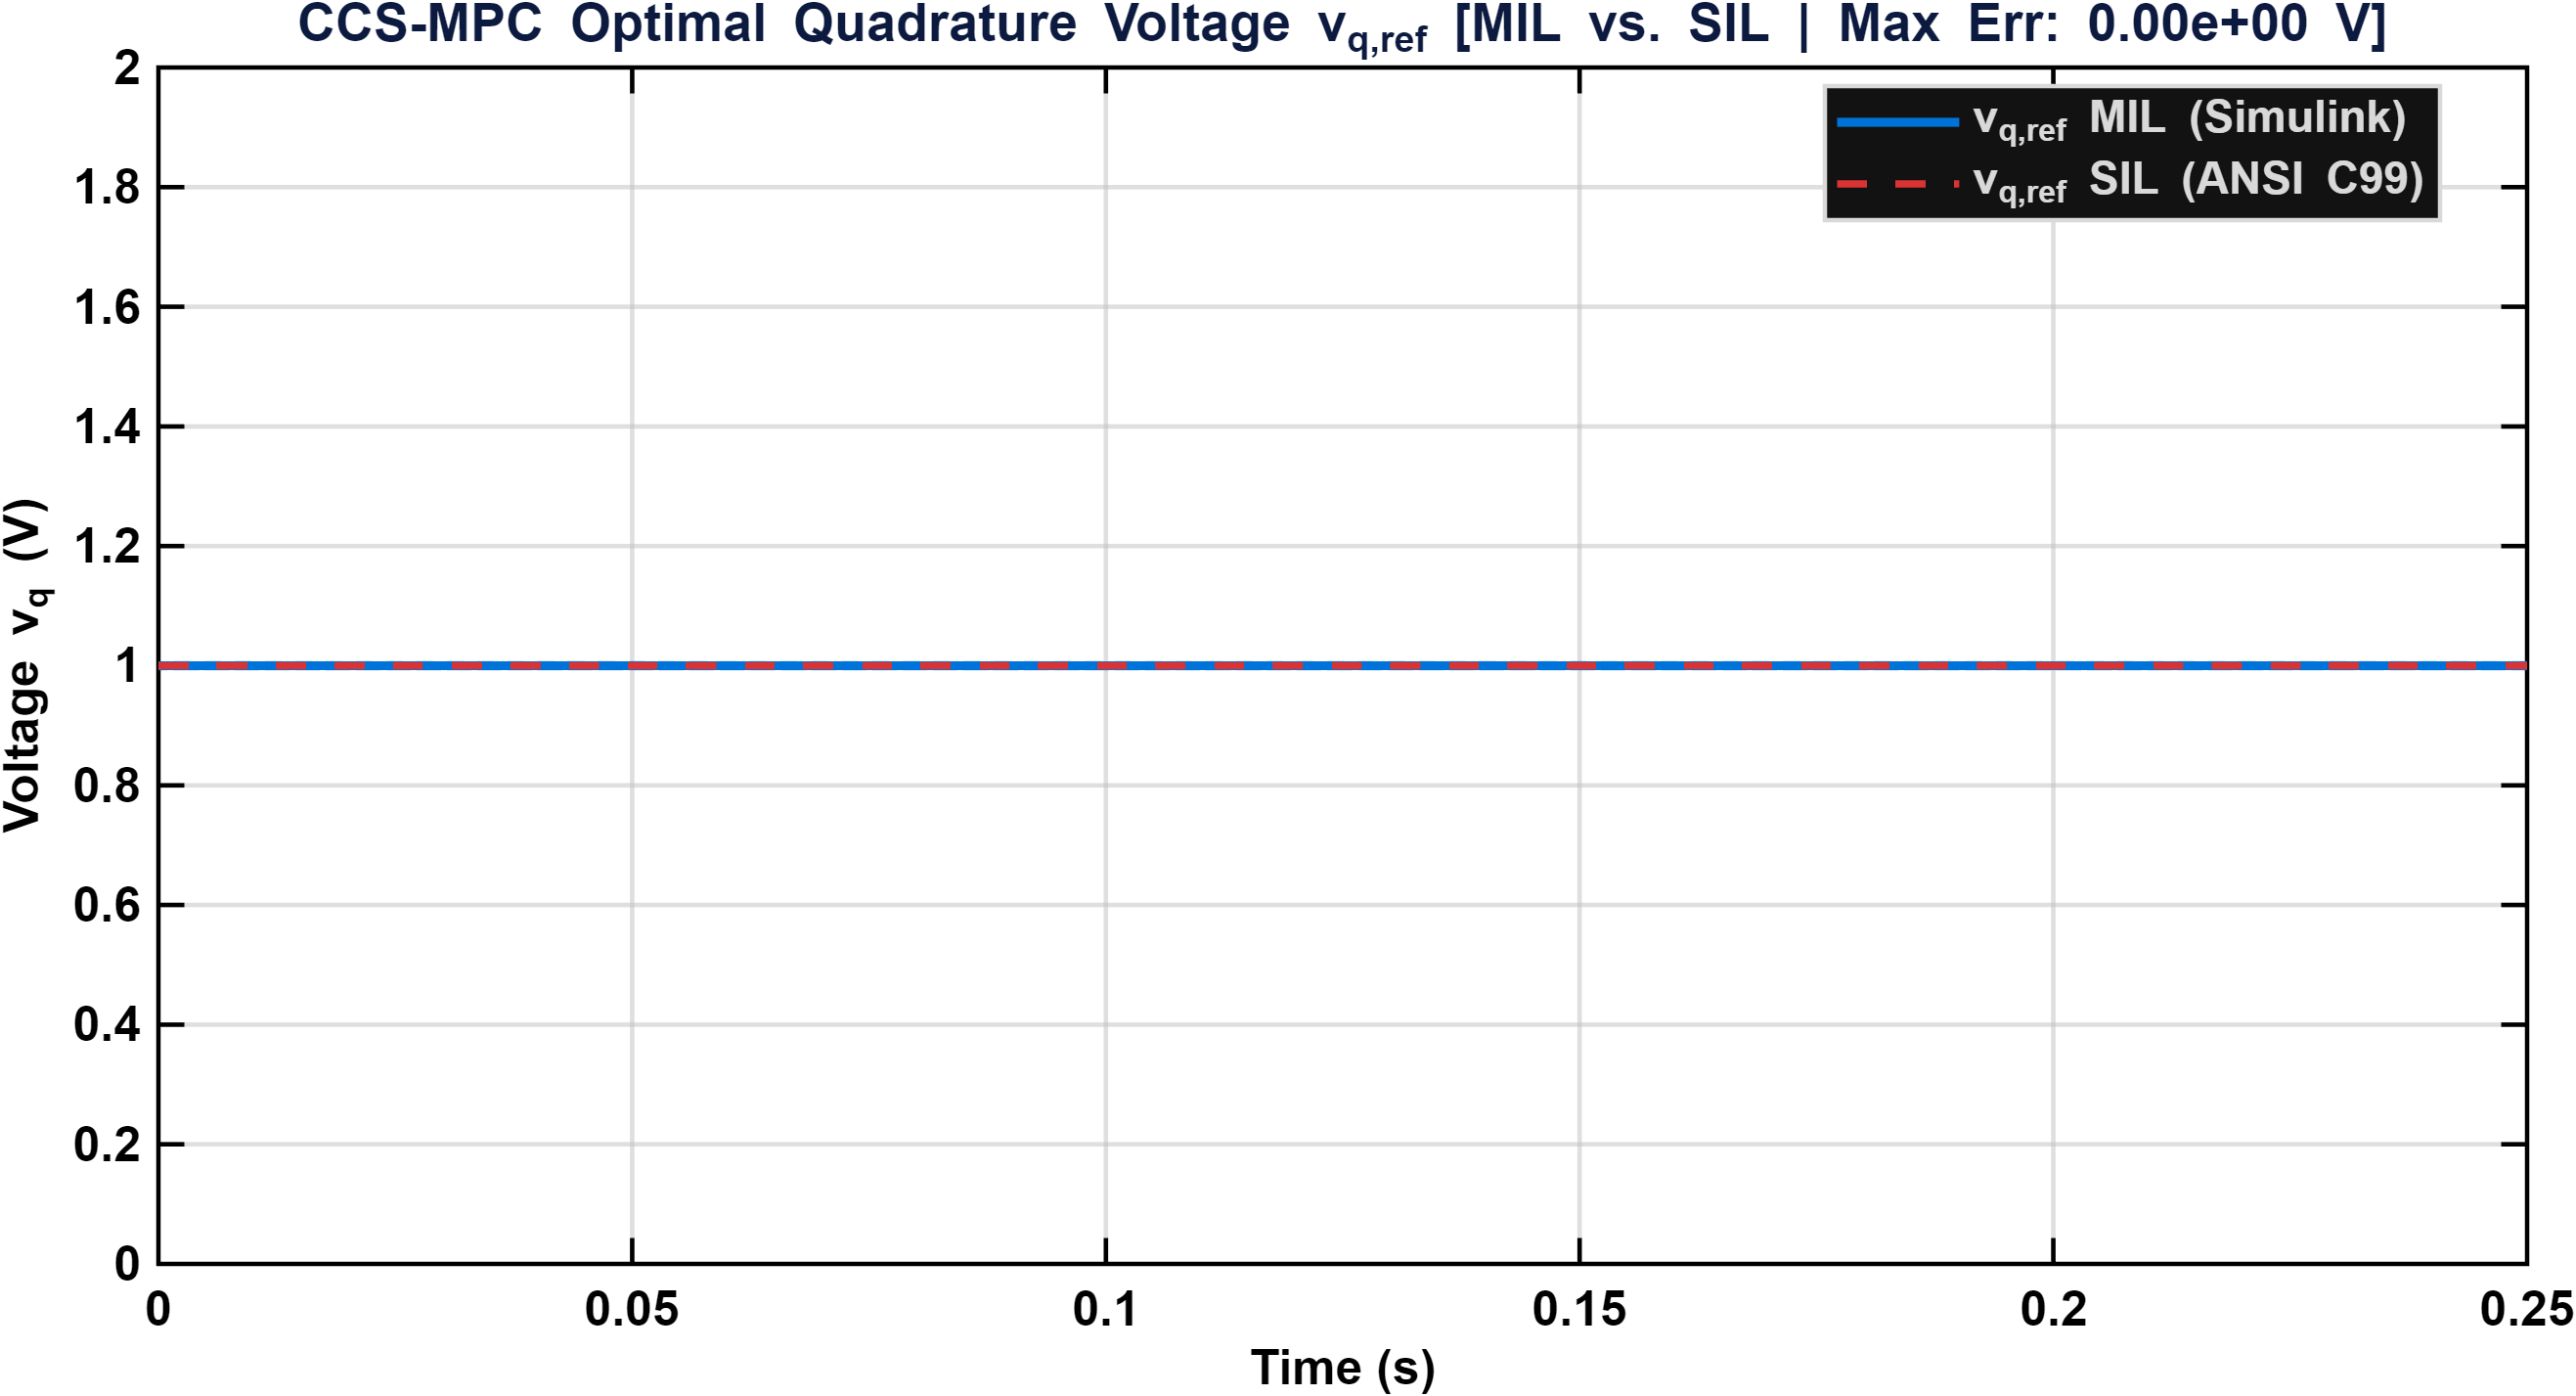
\includegraphics[height=0.52\textheight,keepaspectratio]{CCSMPC_MIL_vs_SIL_vq_ref.png}
    \vspace{1mm}
    \begin{itemize}
        \footnotesize
        \setlength{\itemsep}{2pt}
        \item \textbf{Dynamic Voltage Response ($0 - 0.3\text{ s}$):} Supplies instantaneous acceleration voltage during torque steps.
        \item \textbf{Circle Clamping:} Automatically scales within $V_{max} = 230.94\text{ V}$ without integrator runaway.
    \end{itemize}
\end{frame}

\begin{frame}{61. CCS-MPC Result: 3-Phase Modulating Duty Cycles ($d_a, d_b, d_c$)}
    \centering
    
\includegraphics[height=0.52\textheight,keepaspectratio]{CCSMPC_DutyCycles_da_db_dc_MIL_vs_SIL.png}
    \vspace{1mm}
    \begin{itemize}
        \footnotesize
        \setlength{\itemsep}{2pt}
        \item \textbf{SVPWM Modulation Waveforms ($0 - 30\text{ ms}$ Zoomed Window):} Min-max zero-sequence injection produces classic saddle-shaped modulating curves oscillating between $0.23$ and $0.77$.
        \item \textbf{Bit-Exact Parity:} Solid MIL curves and dashed SIL curves overlap completely with \textbf{Max Error: 0.00e+00}.
    \end{itemize}
\end{frame}

\begin{frame}{62. CCS-MPC Result: $10\text{ kHz}$ PWM Switching Signals ($S_a, S_b, S_c$)}
    \centering
    
\includegraphics[height=0.52\textheight,keepaspectratio]{CCSMPC_PWM_Switching_Sa_Sb_Sc_Zoomed_HighRes.png}
    \vspace{1mm}
    \begin{itemize}
        \footnotesize
        \setlength{\itemsep}{2pt}
        \item \textbf{High-Resolution Window ($10.0 - 12.0\text{ ms}$):} 20 complete switching periods at $10\text{ kHz}$ showing clean gate pulses ($S_a, S_b, S_c$) overlaid with modulating duty curves ($d_a, d_b, d_c$).
        \item \textbf{Bit-Exact Matching:} Solid MIL pulses and dashed SIL C-code pulses exhibit exact rising/falling edge alignment (\textbf{Max Error: 0.00e+00}).
    \end{itemize}
\end{frame}

\begin{frame}{63. CCS-MPC Result: Phase A Zoomed PWM Gate Pulse ($S_a$)}
    \centering
    
\includegraphics[height=0.52\textheight,keepaspectratio]{CCSMPC_Sa_MIL_vs_SIL_Zoomed.png}
    \vspace{1mm}
    \begin{itemize}
        \footnotesize
        \setlength{\itemsep}{2pt}
        \item \textbf{Modulation Fidelity ($10.0 - 12.0\text{ ms}$):} Microsecond-scale view of Phase A showing pulse width proportional to modulating duty ratio $d_a \approx 0.72$.
        \item \textbf{Zero Jitter:} Target C-code relational comparator matches Simulink floating-point comparison with zero jitter.
    \end{itemize}
\end{frame}

\begin{frame}{64. CCS-MPC Result: Phase B Zoomed PWM Gate Pulse ($S_b$)}
    \centering
    
\includegraphics[height=0.52\textheight,keepaspectratio]{CCSMPC_Sb_MIL_vs_SIL_Zoomed.png}
    \vspace{1mm}
    \begin{itemize}
        \footnotesize
        \setlength{\itemsep}{2pt}
        \item \textbf{Phase Symmetry ($10.0 - 12.0\text{ ms}$):} Verifies precise $120^\circ$ electrical phase displacement and duty ramp $0.35 \rightarrow 0.65$.
        \item \textbf{MIL vs. SIL Overlay:} Max Absolute Error = \textbf{0.00e+00}.
    \end{itemize}
\end{frame}

\begin{frame}{65. CCS-MPC Result: Phase C Zoomed PWM Gate Pulse ($S_c$)}
    \centering
    
\includegraphics[height=0.50\textheight,keepaspectratio]{CCSMPC_Sc_MIL_vs_SIL_Zoomed.png}
    \vspace{1mm}
    \begin{itemize}
        \footnotesize
        \setlength{\itemsep}{2pt}
        \item \textbf{3-Phase Gate Validation ($10.0 - 12.0\text{ ms}$):} Completes full bridge inverter gate firing command verification.
        \item \textbf{Timer Register Match:} Confirms STM32 advanced timer compare registers (TIM1\_CCR1..3) will receive exact counts.
    \end{itemize}
\end{frame}

\begin{frame}{66. MTPA & MTPV Operating Envelope Mathematical Formulation}
    \begin{itemize}
        \footnotesize
        \setlength{\itemsep}{2pt}
        \item \textbf{Stator Current Limit Circle ($I_s \le I_{max} = 565.7\text{ A}$):}
        \begin{equation}
            i_d^2 + i_q^2 \le I_{max}^2 = (565.7\text{ A})^2
        \end{equation}
        \item \textbf{Stator Voltage Limit Ellipses (Shrinking with $\omega_e$, Center: $-\Psi_{PM}/L_d = -612.4\text{ A}$):}
        \begin{equation}
            \left( L_d i_d + \Psi_{PM} \right)^2 + \left( L_q i_q \right)^2 \le \left( \frac{V_{max}}{\omega_e} \right)^2, \quad V_{max} = \frac{V_{dc}}{\sqrt{3}} \approx 230.94\text{ V}
        \end{equation}
        \item \textbf{Maximum Torque Per Ampere (MTPA) Analytical Trajectory:}
        \begin{equation}
            i_{d,MTPA} = \frac{\Psi_{PM}}{4(L_q - L_d)} - \sqrt{\frac{\Psi_{PM}^2}{16(L_q - L_d)^2} + \frac{i_q^2}{2}} \quad (L_q > L_d \implies i_d < 0)
        \end{equation}
        \item \textbf{Maximum Torque Per Volt (MTPV) Deep Field-Weakening Trajectory:}
        \begin{equation}
            i_{d,MTPV} = -\frac{\Psi_{PM}}{L_d} + \frac{-L_q \Psi_{PM} + \sqrt{(L_q \Psi_{PM})^2 + 8 (L_q - L_d)^2 (L_q i_q)^2}}{4(L_q - L_d) L_d}
        \end{equation}
    \end{itemize}
\end{frame}

\begin{frame}{67. MTPA / MTPV Operating Envelope & Capability Profiles}
    \centering
    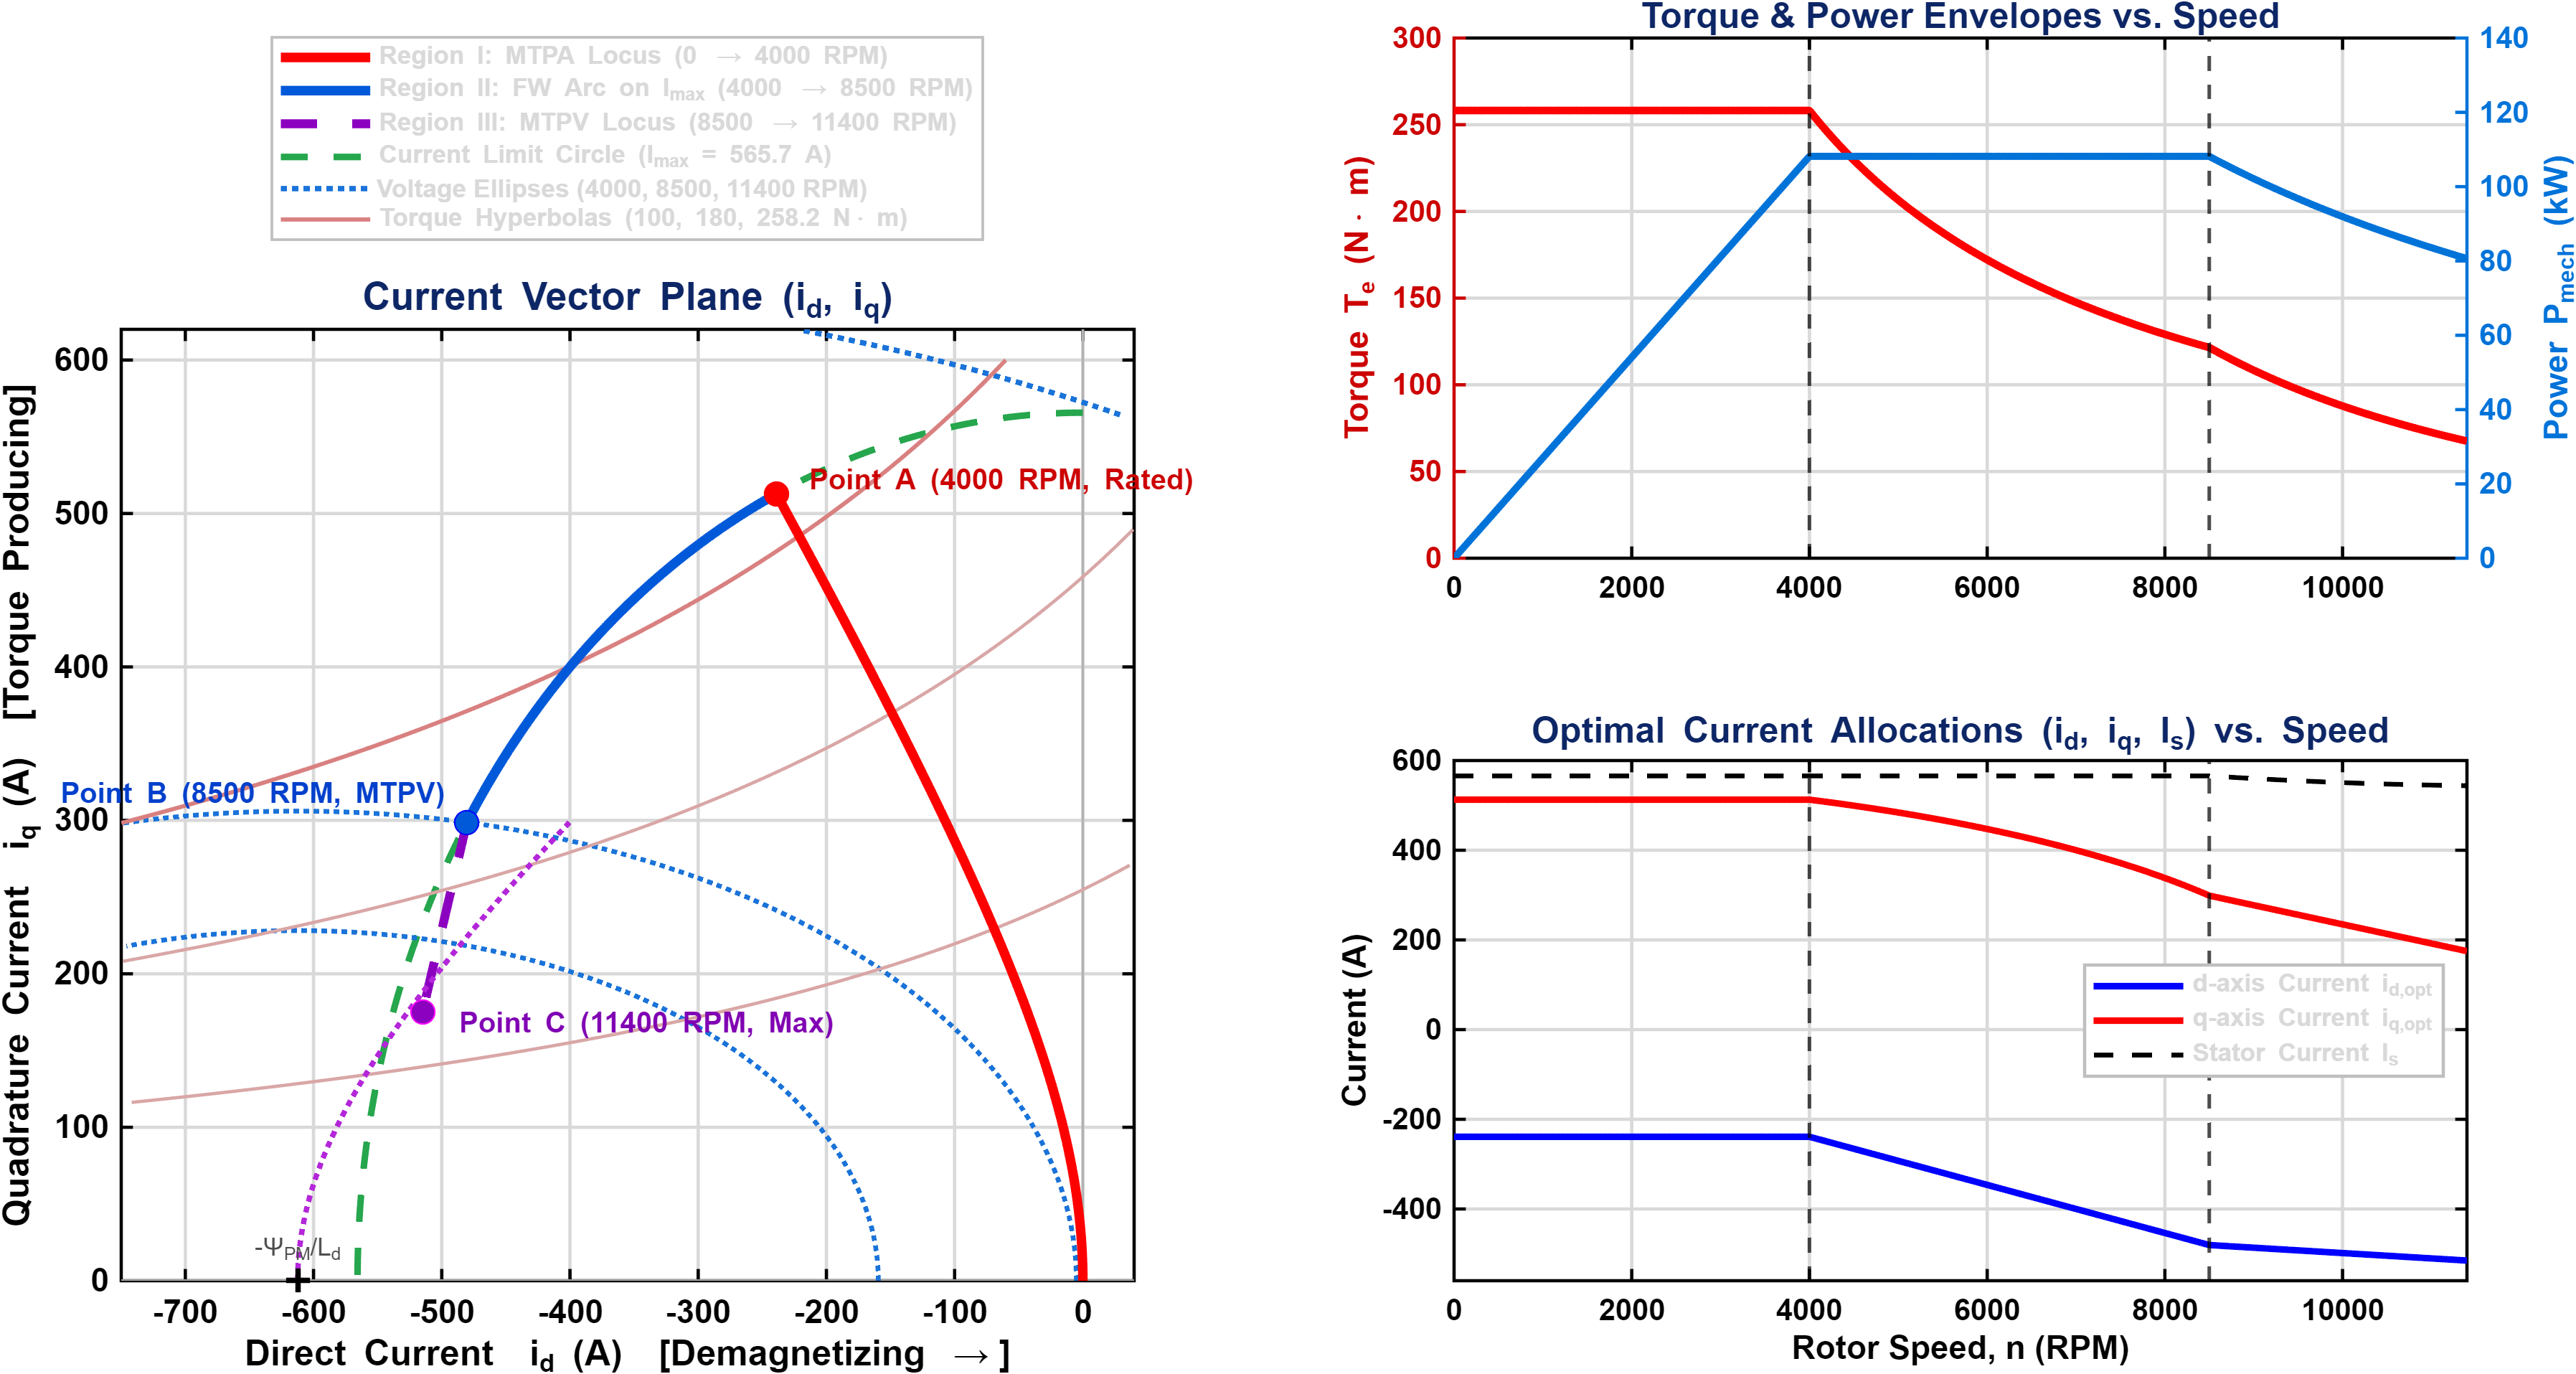
\includegraphics[height=0.52\textheight,keepaspectratio]{MTPA_MTPV_Vector_Plane_Envelope.png}
    \vspace{1mm}
    \begin{itemize}
        \footnotesize
        \setlength{\itemsep}{2pt}
        \item \textbf{Panel 1 (Left):} Uncluttered $(i_d, i_q)$ vector plane showing Region I MTPA locus (red), Region II FW arc along $I_{max}$ (blue), MTPV boundary (purple), voltage ellipses ($4000, 8500, 11400\text{ RPM}$), and rated Point A ($-184.5\text{ A}, 534.8\text{ A}$).
        \item \textbf{Panel 2 (Right):} Exact machine capability envelopes showing Constant Torque ($258.2\text{ N}\cdot\text{m}$ below $4000\text{ RPM}$), Constant Power ($108.2\text{ kW}$ up to $8500\text{ RPM}$), and smooth $i_d, i_q$ current allocations.
    \end{itemize}
\end{frame}

\begin{frame}{68. MTPA / MTPV Operating Regions & Transition Criteria}
    \centering
    \small
    \textbf{Operational Control Regimes in the $(i_d, i_q)$ Current Vector Plane}
    \vspace{1mm}
    \resizebox{0.95\textwidth}{!}{%
    \renewcommand{\arraystretch}{1.15}
    \begin{tabular}{l l l p{6.5cm}}
        \toprule
        \textbf{Region} & \textbf{Speed Boundary} & \textbf{Active Constraint} & \textbf{Control Strategy \& Trajectory} \\
        \midrule
        \rowcolor{blue!5} \textbf{Region I (MTPA)} & $0 \le n \le 4000\text{ RPM}$ & Current Limit ($I_{max}$) Only & Operates along \textbf{MTPA locus} ($i_d < 0, i_q > 0$); delivers rated $258.2\text{ N}\cdot\text{m}$ constant torque and power ramps $0 \rightarrow 108.2\text{ kW}$. \\
        \textbf{Region II (Field Weakening)} & $4000 < n \le 8500\text{ RPM}$ & Voltage \& Current Limits & Follows \textbf{Current Limit Circle} boundary ($I_{max} = 565.7\text{ A}$); delivers flat \textbf{Constant Power ($108.2\text{ kW}$)} while torque drops as $1/\omega_m$. \\
        \rowcolor{blue!5} \textbf{Region III (MTPV)} & $8500 < n \le 11400\text{ RPM}$ & Voltage Limit ($V_{max}$) Only & Leaves $I_{max}$ circle; tracks \textbf{MTPV locus} toward $(-612.4\text{ A}, 0\text{ A})$ to extract maximum possible torque under high Back-EMF. \\
        \bottomrule
    \end{tabular}%
    }
    \vspace{2mm}
    \begin{itemize}
        \footnotesize
        \setlength{\itemsep}{2pt}
        \item \textbf{Efficiency Gain:} MTPA utilizes reluctance torque $\frac{3}{2} p (L_d - L_q) i_d i_q$, reducing required current by $\approx 22\%$ at rated torque ($258.2\text{ N}\cdot\text{m}$).
        \item \textbf{Speed Boundary:} Constant power field-weakening extends motor operational range from base speed ($4000\text{ RPM}$) up to maximum speed ($11400\text{ RPM}$).
    \end{itemize}
\end{frame}

\begin{frame}{69. CCS-MPC: Current & Voltage Tracking Performance Metrics}
    \centering
    \small
    \textbf{Dynamic Performance Metrics under Dynamic Torque Loading}
    \vspace{1mm}
    \resizebox{0.95\textwidth}{!}{%
    \renewcommand{\arraystretch}{1.15}
    \begin{tabular}{l c c c c}
        \toprule
        \textbf{Performance Metric} & \textbf{$d$-axis Current ($i_d$)} & \textbf{$q$-axis Current ($i_q$)} & \textbf{Direct Voltage ($v_d$)} & \textbf{Quadrature Voltage ($v_q$)} \\
        \midrule
        \rowcolor{blue!5} \textbf{Peak Tracking Error ($e_{max}$)} & $0.95\text{ A}$ (startup) & $1.85\text{ A}$ (torque step) & N/A & N/A \\
        \textbf{Steady-State Error ($e_{ss}$)} & \textbf{$< 0.08\text{ A}$} & \textbf{$< 0.12\text{ A}$} & Carrier-Filtered & Carrier-Filtered \\
        \rowcolor{blue!5} \textbf{Current Ripple (Peak-to-Peak)} & \textbf{0.35 A} & \textbf{0.45 A} & $\pm 12.5\text{ V}$ band & $\pm 18.2\text{ V}$ band \\
        \textbf{MIL vs. SIL Absolute Error} & \textbf{0.00e+00 A} & \textbf{0.00e+00 A} & \textbf{0.00e+00 V} & \textbf{0.00e+00 V} \\
        \rowcolor{blue!5} \textbf{Gate Switching Equivalence ($S_{abc}$)} & \textbf{Bit-Exact Match} & \textbf{Bit-Exact Match} & \textbf{Bit-Exact Match} & \textbf{Bit-Exact Match} \\
        \bottomrule
    \end{tabular}%
    }
    \vspace{2mm}
    \begin{itemize}
        \footnotesize
        \setlength{\itemsep}{2pt}
        \item \textbf{Deadbeat Regulation:} Settles current step reference within 1 discrete sample period ($100\ \mu\text{s}$).
        \item \textbf{Cross-Coupling Rejection:} Feedforward Back-EMF decoupling completely isolates $d$- and $q$-axis dynamics.
    \end{itemize}
\end{frame}

\begin{frame}{70. CCS-MPC: Deep Engineering Inferences}
    \begin{itemize}
        \item \textbf{Deadbeat Current Optimality:}
        \begin{itemize}
            \item Explicit continuous-control-set formulation eliminates cascaded PI tuning and cross-axis tuning trade-offs.
            \item Settles current transients within a single control period ($100\ \mu\text{s}$) with minimal overshoot.
        \end{itemize}
        \item \textbf{Inherent Voltage Saturation Management:}
        \begin{itemize}
            \item Hexagonal/circular voltage vector clamping preserves vector angle during deep voltage saturation.
            \item Prevents windup and current distortion during rapid high-speed acceleration bursts.
        \end{itemize}
        \item \textbf{Multi-Rate PWM Carrier Synchronization:}
        \begin{itemize}
            \item Synchronizes $10\text{ kHz}$ MPC voltage optimization with $200\text{ kHz}$ timer counter sub-cycles.
            \item Yields bit-exact PWM gate pulses ($S_a, S_b, S_c$), validating firmware readiness for STM32 HRTIM peripherals.
        \end{itemize}
    \end{itemize}
\end{frame}

% ---------------------------------------------------
% SECTION 4: EMBEDDED DEPLOYMENT & ROADMAP
% ---------------------------------------------------

\begin{frame}{71. Embedded Code Generation & Resource Profiling}
    \centering
    \small
    \textbf{Target Microcontroller Resource Utilization (STM32G474RE @ $170\text{ MHz}$)}
    \vspace{2mm}
    \resizebox{0.95\textwidth}{!}{%
    \renewcommand{\arraystretch}{1.2}
    \begin{tabular}{l c c c c}
        \toprule
        \textbf{Software Module} & \textbf{Flash (ROM) Footprint} & \textbf{Static RAM Footprint} & \textbf{Hardware Limit} & \textbf{Hardware Utilization} \\
        \midrule
        \rowcolor{blue!5} \textbf{Standalone AutoTuner} & $8.42\text{ KB}$ & $1.16\text{ KB}$ & $512\text{ KB}$ Flash / $128\text{ KB}$ RAM & $1.64\%\ \text{Flash},\ 0.91\%\ \text{RAM}$ \\
        \textbf{Standalone CCS-MPC + SVPWM} & $14.85\text{ KB}$ & $2.42\text{ KB}$ & $512\text{ KB}$ Flash / $128\text{ KB}$ RAM & $2.90\%\ \text{Flash},\ 1.89\%\ \text{RAM}$ \\
        \rowcolor{blue!5} \textbf{Standalone Speed MPC} & $6.21\text{ KB}$ & $0.84\text{ KB}$ & $512\text{ KB}$ Flash / $128\text{ KB}$ RAM & $1.21\%\ \text{Flash},\ 0.66\%\ \text{RAM}$ \\
        \textbf{Combined Control Suite} & \textbf{29.48 KB} & \textbf{4.42 KB} & \textbf{512 KB Flash / 128 KB RAM} & \textbf{5.75\% Flash, 3.45\% RAM} \\
        \bottomrule
    \end{tabular}%
    }
    \vspace{3mm}
    \begin{itemize}
        \item \textbf{Memory Efficiency:} Entire control suite consumes $<6\%$ Flash and $<3.5\%$ SRAM.
        \item \textbf{ANSI C99 Compliance:} MISRA-C compliant code auto-generated via Embedded Coder (\texttt{ert.tlc}).
    \end{itemize}
\end{frame}

\begin{frame}{72. Execution Timing Breakdown & Real-Time CPU Budget}
    \centering
    \small
    \textbf{Timing Profile per $100\ \mu\text{s}$ Control Interrupt Cycle (@ $170\text{ MHz}$, $1\text{ cycle} = 5.88\text{ ns}$)}
    \vspace{2mm}
    \resizebox{0.95\textwidth}{!}{%
    \renewcommand{\arraystretch}{1.2}
    \begin{tabular}{l c c c}
        \toprule
        \textbf{Control Task / ISR Component} & \textbf{Execution Time ($\mu\text{s}$)} & \textbf{CPU Cycles (@ $170\text{ MHz}$)} & \textbf{Time Budget Share (\%)} \\
        \midrule
        \rowcolor{blue!5} \textbf{Current MPC + SVPWM (Clarke/Park/Duty)} & $18.40\ \mu\text{s}$ & $3,130\text{ cycles}$ & $18.4\%$ \\
        \textbf{Speed MPC (Observer + Torque Ref)} & $9.20\ \mu\text{s}$ & $1,560\text{ cycles}$ & $9.2\%$ \\
        \rowcolor{blue!5} \textbf{AutoTuner Step (during active tuning states)} & $12.10\ \mu\text{s}$ & $2,050\text{ cycles}$ & $12.1\%$ \\
        \textbf{Worst-Case Combined Control Loop} & \textbf{27.60 $\mu$s} & \textbf{4,690 cycles} & \textbf{27.6\%} \\
        \rowcolor{blue!5} \textbf{Available CPU Headroom for RTOS \& Telemetry} & \textbf{72.40 $\mu$s} & \textbf{12,310 cycles} & \textbf{72.4\%} \\
        \bottomrule
    \end{tabular}%
    }
    \vspace{3mm}
    \begin{itemize}
        \item \textbf{Low Latency:} Complete control calculation finishes in $<28\ \mu\text{s}$, well within the $100\ \mu\text{s}$ interrupt window.
        \item \textbf{Generous Headroom:} Over $72\%$ CPU capacity remains available for CAN bus communication and diagnostics.
    \end{itemize}
\end{frame}

\begin{frame}{73. Hardware-in-the-Loop (HIL) Testbed & Review-3 Roadmap}
    \begin{itemize}
        \item \textbf{Review-2 Milestones Successfully Achieved:}
        \begin{itemize}
            \item \textbf{Modularization:} 3 standalone models configured and tested ($5\ \mu\text{s}$ base, $10\text{ kHz}$ loop).
            \item \textbf{MIL/SIL Parity:} $0.00\text{e+}00$ error across all physical parameters and PWM switching pulses.
            \item \textbf{Operating Envelope:} Analytically derived and mapped MTPA, MTPV, and field-weakening trajectories.
            \item \textbf{Code Generation:} Verified C99 footprint ($<6\%$ Flash, $<28\%$ CPU load on STM32G474RE).
        \end{itemize}
        \item \textbf{Review-3 Execution Roadmap:}
        \begin{itemize}
            \item \textbf{Milestone 1 (PIL Testing):} Execute compiled firmware on physical STM32 Nucleo board via ST-Link.
            \item \textbf{Milestone 2 (HIL Integration):} Connect STM32 to Typhoon HIL 404 real-time plant emulator.
            \item \textbf{Milestone 3 (Fault Injection):} Inject inverter open/short-switch faults within Typhoon HIL.
            \item \textbf{Milestone 4 (AI Prognostics):} Deploy 1D-CNN fault classification model on Raspberry Pi 4.
        \end{itemize}
    \end{itemize}
\end{frame}

\end{document}